\immediate\write18{makeindex \jobname.nlo -s nomentbl.ist -o \jobname.nls}
\immediate\write18{makeglossaries \jobname}

\documentclass{skripsi}

%Jika ingin menambahkan command baru, harap ditambahkan di file 'my_command'
\usepackage{colortbl}  %--- untuk membuat tabel berwarna
\usepackage{listings}  %--- untuk menulis listing program
\usepackage{xcolor}    %--- memanfaatkan warna LaTeX
\usepackage{caption}
\usepackage{color}
\usepackage{lscape}
\usepackage{amsmath}
\usepackage{amsfonts}
\usepackage{commath}
\usepackage{chemarr}
\usepackage{nomencl}
\usepackage{etoolbox}
% \usepackage{eufrak}
% \usepackage{arrayjob}
% \usepackage{arrayjobx}

\usepackage{hyperref}
\urlstyle{rm}
\renewcommand\UrlFont{\rmfamily\itshape}
% \hypersetup{
%     pdftitle={Draft Tugas Akhir - Syahrul Rofi - 10115077},
%     bookmarks=true,
%     }
%\usepackage[printwatermark]{xwatermark}
%\usepackage{draftwatermark} %\usepackage[firstpage]{draftwatermark}

\usepackage{booktabs}  % untuk tabel
\usepackage{longtable}
%\usepackage{tabularx}
\usepackage{tabu}
%\usepackage{subfigure}
\usepackage{subcaption}
\usepackage{multicol}
\usepackage{multirow}
%\usepackage{sectsty}
%\usepackage{lipsum}
\usepackage{graphicx}
%\usepackage{latexsym}
%\usepackage{float}
\usepackage{array}
%\usepackage{mathrsfs}%
%\usepackage{lineno}
\usepackage{relsize} %modifikasi ukuran operator matematika
\usepackage{amssymb}
\usepackage[decimalsymbol=comma]{siunitx} %dapat mengganti simbol desimal dengan koma

\usepackage{tikz}
\usepackage{mathtools}
\usepackage{pgfplots}
\pgfplotsset{compat=1.15}

\usepackage{pgffor}
\usepackage{xparse}
\usepackage{keyval}
\usepackage{pgfmath}

\usepackage[toc]{appendix}
\usepackage{fancyhdr}
%%%%%%%%%%%%%%%%%%%%%%%%%%%%%%%%%%%%%%%%%%%%%%%%%%%%%%%%%%%%%
\definecolor{abu}{gray}{0.80}  % = hitam 20%

\newcommand{\cca}{\cellcolor{abu}}
\newcommand{\ccb}{\bfseries}

\newcolumntype{L}[1]{>{\raggedright\let\newline\\\arraybackslash\hspace{0pt}}m{#1}}
\newcolumntype{P}[1]{>{\raggedright\let\newline\\\arraybackslash\hspace{0pt}}p{#1}}
\newcolumntype{C}[1]{>{\centering\let\newline\\\arraybackslash\hspace{0pt}}m{#1}}
\newcolumntype{Q}[1]{>{\centering\let\newline\\\arraybackslash\hspace{0pt}}p{#1}}
\newcolumntype{R}[1]{>{\raggedleft\let\newline\\\arraybackslash\hspace{0pt}}m{#1}}


\graphicspath{{FolderGambar/}}%----folder tempat gambar-gambar---

\newcommand{\tmatriks}[1]{%
    \bigl(\begin{smallmatrix}#1\end{smallmatrix}\bigr)}

\newtheoremstyle{teoremaku}% --- style untuk teorema dkk
    {4ex}
    {3ex}
    {\itshape}
    {}
    {\bfseries}
    {}
    {1em}
    {}

\newtheoremstyle{contohku}% --- style untuk contoh
    {5ex}
    {3ex}
    {}
    {}
    {\bfseries}
    {}
    {1em}
    {}

\theoremstyle{teoremaku}
\newtheorem{theorem}{Teorema}%[chapter]
\newtheorem{lemma}{Lema}%[chapter]
\newtheorem{conjecture}{Dugaan}[chapter]
\newtheorem{corollary}{Akibat}%[chapter]
\newtheorem{definition}{Definisi}%[chapter]
\newtheorem{open problem}{Masalah Terbuka}[chapter]
\newtheorem{assertion}{Assertion}[chapter]
\newtheorem{prop}{Proposisi}[chapter]
\newtheorem{observation}{Observasi}[chapter]
\newcommand{\ebox}{\ \ $\Box$\vspace{1ex}}
\newcommand{\pr}{{\textbf{Bukti.}}\hspace{0.3cm}}

\theoremstyle{contohku}
\newtheorem{contoh}{Contoh}[chapter]

\newcommand{\maks}{\displaystyle\mathrm{maks}}
\DeclareMathOperator{\tr}{trace}
\DeclareMathOperator{\rank}{rank}
\DeclareMathOperator{\round}{round}

\def\ifEqString#1#2{\def\testa{#1}\def\testb{#2}
    \ifx\testa\testb}

\usetikzlibrary{shapes,shadows,calc}
\usepgflibrary{arrows}
\usetikzlibrary{decorations.shapes}
\usepackage{varwidth}

\tikzset{decorates/.style=
{decorate,decoration={shape backgrounds,shape=circle,shape size=0.35mm,shape sep=2mm}},%
decorateb/.style=
{decorate,decoration={shape backgrounds,shape=circle,shape size=1mm,shape sep=3mm}}
}

%-----Boxes & circle
%-----#1 height, #2 width, #3 name of the node, #4 coordinate
\def\kotakbesar[#1,#2,#3,#4]{%
  \node[draw, rectangle, minimum height=#1, minimum width=#2, rounded corners=3] (#3) at #4 {}; %
}
%-----#1 name of the node, #2 coordinate, #3 label
\def\kotak[#1,#2]#3;{
  \node[draw,rectangle,color=black,rounded corners=3,align=center] (#1) at #2 {#3};
}
\def\bulat[#1,#2]#3;{
  \node[draw,circle,color=black,minimum size=0.8cm,inner sep=0pt,align=center] (#1) at #2 {#3};
}
\def\kotakw[#1,#2]#3;{
  \node[draw,rectangle,color=black,rounded corners=3,align=center, inner sep=2pt,minimum size=0.8cm] (#1) at #2 {\begin{varwidth}{16em}#3\end{varwidth}};
 }
\def\kotakww[#1,#2]#3;{
  \node[draw,rectangle,color=black,rounded corners=3,align=center, inner sep=2pt,minimum size=0.8cm] (#1) at #2 {\begin{varwidth}{10em}#3\end{varwidth}};
 }
\def\kosong[#1,#2]#3;{
  \node (#1) at #2 {\begin{varwidth}{11em}#3\end{varwidth}};
 }%[font=\fontsize{#3}{0}\selectfont]
%-----#3 & #4 label
\def\kotaktl[#1,#2]#3#4;{
  \node[draw,rectangle,color=black,rounded corners=3,align=center] (#1) at #2 {#3\\#4};
}
\def\bulattl[#1,#2]#3#4;{
  \node[draw,circle,color=black,minimum size=0.8cm,inner sep=0pt,align=center] (#1) at #2 {#3\\#4};
}
%-----#1 from node, #2 to node, #3 angle of a node, #4 position of a node, #5 node label
%-----dashed, or other parameters for draw
\def\singleT[#1,#2,#3,#4]#5;{ 
  \draw[-triangle 60,color=black!20!black] (#1) -- (#2) node[midway,sloped,#4,rotate=#3,font=\fontsize{8}{0}\selectfont,text width=2.3cm, align=center] {#5};  
}
\def\singleTf[#1,#2,#3,#4,#5]#6;{ 
  \draw[-triangle 60,color=black!20!black] (#1) -- (#2) node[midway,sloped,#4,rotate=#3,font=\fontsize{#5}{0}\selectfont,text width=2.3cm, align=center] {#6};
}
%%#6 text width
\def\singleTfw[#1,#2,#3,#4,#5,#6]#7;{ 
  \draw[-triangle 60,color=black!20!black] (#1) -- (#2) node[midway,sloped,#4,rotate=#3,font=\fontsize{#5}{0}\selectfont,text width=#6, align=center] {#7};
}
\def\doubleT[#1,#2,#3,#4]#5;{ 
  \draw[triangle 60-triangle 60,color=black!20!black] (#1) -- (#2) node[midway,sloped,#4,rotate=#3,font=\fontsize{8}{0}\selectfont] {#5};  
}
\def\titiks[#1,#2];{ 
  \draw[decorates,fill] (#1) -- (#2);
}
\def\titikb[#1,#2];{ 
  \draw[decorateb,fill] (#1) -- (#2);  
}
%---#1 antecedent variable, #2 antecedent's linguistic value, #3 consequent variable, #4 consequent's linguistic value
%---#5 number of antecedent variables, #6 number of fuzzy rules
\makeatletter

\newtoggle{onerule} %
\newtoggle{tworules} %
\newtoggle{threerules}%
\newtoggle{oneante}%
\newtoggle{twoante}%

\def\setboolflc#1#2{%
\ifEqString{#2}{1}%
    \global\toggletrue{onerule}%
    \global\togglefalse{tworules}%
    \global\togglefalse{threerules}%
\else \ifEqString{#2}{2}%
    \global\toggletrue{tworules}%
    \global\togglefalse{onerule}%
    \global\togglefalse{threerules}%
\else \ifEqString{#2}{3}%
    \global\toggletrue{threerules}%
    \global\togglefalse{onerule}%
    \global\togglefalse{tworules}%
\else %
    \global\togglefalse{threerules}%
    \global\togglefalse{onerule}%
    \global\togglefalse{tworules}%
\fi %

\ifEqString{#1}{1} %
    \global\toggletrue{oneante}%
    \global\togglefalse{twoante}%
\else \ifEqString{#1}{2}%
    \global\toggletrue{twoante}%
    \global\togglefalse{oneante}%
\else %
    \global\togglefalse{oneante}%
    \global\togglefalse{twoante}%
\fi %
}%
%

%---- ZADEH FUZZY RULES
\NewDocumentCommand \generalFrZadeh {O{x}O{A}O{y}O{B}O{n}O{m}}{
\setboolflc{#5}{#6}%
\vspace*{-\baselineskip}
\iftoggle{onerule}{\iftoggle{oneante}{%
        \vspace*{-\baselineskip}
        \begin{alignat*}{4}%
        \Re &: \text{ Jika } &&#1 \text{ adalah } #2 \text{,} &&\text{maka } &&#3 \text{ adalah } #4
        \end{alignat*}%
    }{\iftoggle{twoante}{%
    \vspace*{-\baselineskip}
        \begin{align*}%
            \Re &: \text{ Jika } &&#1_1 \text{ adalah } #2_1 &&\text{ dan } &&#1_2 \text{ adalah } #2_2\text{,}%
            &&\text{maka } &&#3 \text{ adalah } #4
        \end{align*}%
    }{\vspace*{-\baselineskip}
    \begin{align*}%
    \Re &: \text{ Jika } &&#1_1 \text{ adalah } #2_1 \text{,} &&\ldots \text{,} &&#1_#5 \text{ adalah } #2_#5,%
    &&\text{maka } &&#3 \text{ adalah } #4
    \end{align*}%
    }%
    }%
}{\iftoggle{tworules}{\iftoggle{oneante}{%
    \vspace*{-\baselineskip}
        \begin{align*}%
        \Re_1 &: \text{ Jika } &&#1 \text{ adalah } #2_1 \text{,} &&\text{maka } &&#3 \text{ adalah } #4_1\\%
        \Re_2 &: \text{ Jika } &&#1 \text{ adalah } #2_2 \text{,} &&\text{maka } &&#3 \text{ adalah } #4_2
        \end{align*}%
    }{\iftoggle{twoante}{%
    \vspace*{-\baselineskip}
        \begin{align*}%
        \Re_1 &: \text{ Jika } &&#1_1 \text{ adalah } #2_{1,1} &&\text{dan} &&#1_2 \text{ adalah } #2_{1,2},%
        &&\text{maka } &&#3 \text{ adalah } #4_1\\%
        \Re_2 &: \text{ Jika } &&#1_1 \text{ adalah } #2_{2,1} &&\text{dan} &&#1_2 \text{ adalah } #2_{2,2},%
        &&\text{maka } &&#3 \text{ adalah } #4_2
        \end{align*}%
    }{\vspace*{-\baselineskip}
        \begin{align*}%
        \Re_1 &: \text{ Jika } &&#1_1 \text{ adalah } #2_{1,1} \text{,} &&\ldots \text{,} &&#1_#5 \text{ adalah } #2_{1,#5} \text{,}
        &&\text{maka } &&#3 \text{ adalah } #4_1\\%
        \Re_2 &: \text{ Jika } &&#1_1 \text{ adalah } #2_{2,1} \text{,} &&\ldots \text{,} &&#1_#5 \text{ adalah } #2_{2,#5} \text{,}
        &&\text{maka } &&#3 \text{ adalah } #4_2
        \end{align*}%
    }%
    }%
}{\iftoggle{threerules}{\iftoggle{oneante}{%
        \vspace*{-\baselineskip}
        \begin{align*}%
        \Re_1 &: \text{ Jika } &&#1 \text{ adalah } #2_1 \text{,} &&\text{maka } &&#3 \text{ adalah } #4_1\\%
        \Re_2 &: \text{ Jika } &&#1 \text{ adalah } #2_2 \text{,} &&\text{maka } &&#3 \text{ adalah } #4_2\\%
        \Re_#6 &: \text{ Jika } &&#1 \text{ adalah } #2_#6 \text{,} &&\text{maka } &&#3 \text{ adalah } #4_#6
        \end{align*}%
    }{\iftoggle{twoante}{%
    \vspace*{-\baselineskip}
        \begin{align*}%
        \Re_1 &: \text{ Jika } &&#1_1 \text{ adalah } #2_{1,1} &&\text{dan} &&#1_2 \text{ adalah } #2_{1,2},%
        &&\text{maka } &&#3 \text{ adalah } #4_1\\%
        \Re_2 &: \text{ Jika } &&#1_1 \text{ adalah } #2_{2,1} &&\text{dan} &&#1_2 \text{ adalah } #2_{2,2},%
        &&\text{maka } &&#3 \text{ adalah } #4_2\\%
        \Re_#6 &: \text{ Jika } &&#1_1 \text{ adalah } #2_{#6,1} &&\text{dan} &&#1_2 \text{ adalah } #2_{#6,2},%
        &&\text{maka } &&#3 \text{ adalah } #4_#6
        \end{align*}%
    }{\vspace*{-\baselineskip}
        \begin{align*}%
        \Re_1 &: \text{ Jika } &&#1_1 \text{ adalah } #2_{1,1} \text{,} &&\ldots \text{,} &&#1_#5 \text{ adalah } #2_{1,#5} \text{,}
        &&\text{maka } &&#3 \text{ adalah } #4_1\\%
        \Re_2 &: \text{ Jika } &&#1_1 \text{ adalah } #2_{2,1} \text{,} &&\ldots \text{,} &&#1_#5 \text{ adalah } #2_{2,#5} \text{,}
        &&\text{maka } &&#3 \text{ adalah } #4_2\\%
        \Re_#6 &: \text{ Jika } &&#1_1 \text{ adalah } #2_{#6,1} \text{,} &&\ldots \text{,} &&#1_#5 \text{ adalah } #2_{#6,#5} \text{,}
        &&\text{maka } &&#3 \text{ adalah } #4_#6
        \end{align*}%
    }%
    }%
}{\iftoggle{oneante}{%
\vspace*{-\baselineskip}
        \begin{align*}%
        \Re_1 &: \text{ Jika } &&#1 \text{ adalah } #2_1 \text{,} &&\text{maka } &&#3 \text{ adalah } #4_1\\%
        \Re_2 &: \text{ Jika } &&#1 \text{ adalah } #2_2 \text{,} &&\text{maka } &&#3 \text{ adalah } #4_2\\%
        & &&\vdots \\
        \Re_#6 &: \text{ Jika } &&#1 \text{ adalah } #2_#6 \text{,} &&\text{maka } &&#3 \text{ adalah } #4_#6
        \end{align*}%
    }{\iftoggle{twoante}{%
    \vspace*{-\baselineskip}
        \begin{align*}%
        \Re_1 &: \text{ Jika } &&#1_1 \text{ adalah } #2_{1,1} &&\text{dan} &&#1_2 \text{ adalah } #2_{1,2},%
        &&\text{maka } &&#3 \text{ adalah } #4_1\\%
        \Re_2 &: \text{ Jika } &&#1_1 \text{ adalah } #2_{2,1} &&\text{dan} &&#1_2 \text{ adalah } #2_{2,2},%
        &&\text{maka } &&#3 \text{ adalah } #4_2\\%
        & && &&\vdots \\
        \Re_#6 &: \text{ Jika } &&#1_1 \text{ adalah } #2_{#6,1} &&\text{dan} &&#1_2 \text{ adalah } #2_{#6,2},%
        &&\text{maka } &&#3 \text{ adalah } #4_#6
        \end{align*}%
    }{\vspace*{-\baselineskip}
        \begin{align*}%
        \Re_1 &: \text{ Jika } &&#1_1 \text{ anggota } #2_{1,1} \text{,} &&\ldots \text{,} &&#1_#5 \text{ anggota } #2_{1,#5} \text{,}
        &&\text{maka } &&#3 \text{ anggota } #4_1\\%
        \Re_2 &: \text{ Jika } &&#1_1 \text{ anggota } #2_{2,1} \text{,} &&\ldots \text{,} &&#1_#5 \text{ anggota } #2_{2,#5} \text{,}
        &&\text{maka } &&#3 \text{ anggota } #4_2\\%
        & && &&\vdots \\
        \Re_#6 &: \text{ Jika } &&#1_1 \text{ anggota } #2_{#6,1} \text{,} &&\ldots \text{,} &&#1_#5 \text{ anggota } #2_{#6,#5} \text{,}
        &&\text{maka } &&#3 \text{ anggota } #4_#6
        \end{align*}%
    }%
    }%
}%
}%
}%
}%

%---TSK FUZZY RULES
\NewDocumentCommand\generalFrTSK{O{x}O{A}O{y}O{b}O{n}O{m}}{%
\setboolflc{#5}{#6}%
\vspace*{-\baselineskip}
\iftoggle{onerule}{\iftoggle{oneante}{%
        \vspace*{-\baselineskip}
        \begin{alignat*}{4}%
        \Re &: \text{ Jika } &&#1 \text{ adalah } #2 \text{,} &&\text{maka } &&#3 = #4_0 + #4_1#1%
        \end{alignat*}%
    }{\iftoggle{twoante}{%
    \vspace*{-\baselineskip}
        \begin{align*}%
            \Re &: \text{ Jika } &&#1_1 \text{ adalah } #2_1 &&\text{ dan } &&#1_2 \text{ adalah } #2_2\text{,}%
            &&\text{maka } &&#3 = \Vec{#4}\cdot \Vec{#1}%
        \end{align*}%
    }{\vspace*{-\baselineskip}
    \begin{align*}%
    \Re &: \text{ Jika } &&#1_1 \text{ adalah } #2_1 \text{,} &&\ldots \text{,} &&#1_#5 \text{ adalah } #2_#5,%
    &&\text{maka } &&#3 = \Vec{#4}\cdot \Vec{#1}%
    \end{align*}%
    }%
    }%
}{\iftoggle{tworules}{\iftoggle{oneante}{%
    \vspace*{-\baselineskip}
        \begin{align*}%
        \Re_1 &: \text{ Jika } &&#1 \text{ adalah } #2_1 \text{,} &&\text{maka } &&#3_1 = #4_{1,0}+#4_{1,1}#1\\%
        \Re_2 &: \text{ Jika } &&#1 \text{ adalah } #2_2 \text{,} &&\text{maka } &&#3_2 = #4_{2,0}+#4_{2,1}#1%
        \end{align*}%
    }{\iftoggle{twoante}{%
    \vspace*{-\baselineskip}
        \begin{align*}%
        \Re_1 &: \text{ Jika } &&#1_1 \text{ adalah } #2_{1,1} &&\text{dan} &&#1_2 \text{ adalah } #2_{1,2},%
        &&\text{maka } &&#3_1 = \Vec{#4_1}\cdot \Vec{#1}\\%
        \Re_2 &: \text{ Jika } &&#1_1 \text{ adalah } #2_{2,1} &&\text{dan} &&#1_2 \text{ adalah } #2_{2,2},%
        &&\text{maka } &&#3_2 = \Vec{#4_2}\cdot \Vec{#1}%
        \end{align*}%
    }{\vspace*{-\baselineskip}
        \begin{align*}%
        \Re_1 &: \text{ Jika } &&#1_1 \text{ adalah } #2_{1,1} \text{,} &&\ldots \text{,} &&#1_#5 \text{ adalah } #2_{1,#5} \text{,}
        &&\text{maka } &&#3_1 = \Vec{#4_1}\cdot \Vec{#1}\\%
        \Re_2 &: \text{ Jika } &&#1_1 \text{ adalah } #2_{2,1} \text{,} &&\ldots \text{,} &&#1_#5 \text{ adalah } #2_{2,#5} \text{,}
        &&\text{maka } &&#3_2 = \Vec{#4_2}\cdot \Vec{#1}%
        \end{align*}%
    }%
    }%
}{\iftoggle{threerules}{\iftoggle{oneante}{%
        \vspace*{-\baselineskip}
        \begin{align*}%
        \Re_1 &: \text{ Jika } &&#1 \text{ adalah } #2_1 \text{,} &&\text{maka } &&#3_1 = #4_{1,0}+#4_{1,1}#1\\%
        \Re_2 &: \text{ Jika } &&#1 \text{ adalah } #2_2 \text{,} &&\text{maka } &&#3_2 = #4_{2,0}+#4_{2,1}#1\\%
        \Re_#6 &: \text{ Jika } &&#1 \text{ adalah } #2_#6 \text{,} &&\text{maka } &&#3_#6 = #4_{#6,0}+#4_{#6,1}#1%
        \end{align*}%
    }{\iftoggle{twoante}{%
    \vspace*{-\baselineskip}
        \begin{align*}%
        \Re_1 &: \text{ Jika } &&#1_1 \text{ adalah } #2_{1,1} &&\text{dan} &&#1_2 \text{ adalah } #2_{1,2},%
        &&\text{maka } &&##3_1 = \Vec{#4_1}\cdot \Vec{#1}\\%
        \Re_2 &: \text{ Jika } &&#1_1 \text{ adalah } #2_{2,1} &&\text{dan} &&#1_2 \text{ adalah } #2_{2,2},%
        &&\text{maka } &&#3_2 = \Vec{#4_2}\cdot \Vec{#1}\\%
        \Re_#6 &: \text{ Jika } &&#1_1 \text{ adalah } #2_{#6,1} &&\text{dan} &&#1_2 \text{ adalah } #2_{#6,2},%
        &&\text{maka } &&#3_#6 = \Vec{#4_#6}\cdot \Vec{#1}%
        \end{align*}%
    }{\vspace*{-\baselineskip}
        \begin{align*}%
        \Re_1 &: \text{ Jika } &&#1_1 \text{ adalah } #2_{1,1} \text{,} &&\ldots \text{,} &&#1_#5 \text{ adalah } #2_{1,#5} \text{,}
        &&\text{maka } &&#3_1 = \Vec{#4_1}\cdot \Vec{#1}\\%
        \Re_2 &: \text{ Jika } &&#1_1 \text{ adalah } #2_{2,1} \text{,} &&\ldots \text{,} &&#1_#5 \text{ adalah } #2_{2,#5} \text{,}
        &&\text{maka } &&#3_2 = \Vec{#4_2}\cdot \Vec{#1}\\%
        \Re_#6 &: \text{ Jika } &&#1_1 \text{ adalah } #2_{#6,1} \text{,} &&\ldots \text{,} &&#1_#5 \text{ adalah } #2_{#6,#5} \text{,}
        &&\text{maka } &&#3_#6 = \Vec{#4_#6}\cdot \Vec{#1}%
        \end{align*}%
    }%
    }%
}{\iftoggle{oneante}{%
\vspace*{-\baselineskip}
        \begin{align*}%
        \Re_1 &: \text{ Jika } &&#1 \text{ adalah } #2_1 \text{,} &&\text{maka } &&#3_1 = #4_{1,0}+#4_{1,1}#1\\%
        \Re_2 &: \text{ Jika } &&#1 \text{ adalah } #2_2 \text{,} &&\text{maka } &&#3_2 = #4_{2,0}+#4_{2,1}#1\\%
        & &&\vdots \\
        \Re_#6 &: \text{ Jika } &&#1 \text{ adalah } #2_#6 \text{,} &&\text{maka } &&#3_#6 = #4_{#6,0}+#4_{#6,1}#1%
        \end{align*}%
    }{\iftoggle{twoante}{%
    \vspace*{-\baselineskip}
        \begin{align*}%
        \Re_1 &: \text{ Jika } &&#1_1 \text{ adalah } #2_{1,1} &&\text{dan} &&#1_2 \text{ adalah } #2_{1,2},%
        &&\text{maka } &&#3_1 = \Vec{#4_1}\cdot \Vec{#1}\\%
        \Re_2 &: \text{ Jika } &&#1_1 \text{ adalah } #2_{2,1} &&\text{dan} &&#1_2 \text{ adalah } #2_{2,2},%
        &&\text{maka } &&#3_2 = \Vec{#4_2}\cdot \Vec{#1}\\%
        & && &&\vdots \\
        \Re_#6 &: \text{ Jika } &&#1_1 \text{ adalah } #2_{#6,1} &&\text{dan} &&#1_2 \text{ adalah } #2_{#6,2},%
        &&\text{maka } &&#3_#6 = \Vec{#4_#6}\cdot \Vec{#1}%
        \end{align*}%
    }{\vspace*{-\baselineskip}
        \begin{align*}%
        \Re_1 &: \text{ Jika } &&#1_1 \text{ anggota } #2_{1,1} \text{,} &&\ldots \text{,} &&#1_#5 \text{ anggota } #2_{1,#5} \text{,}
        &&\text{maka } &&#3_1 = \mathbf{#4}_1\cdot \mathbf{\Tilde{#1}}\\%
        \Re_2 &: \text{ Jika } &&#1_1 \text{ anggota } #2_{2,1} \text{,} &&\ldots \text{,} &&#1_#5 \text{ anggota } #2_{2,#5} \text{,}
        &&\text{maka } &&#3_2 = \mathbf{#4}_2\cdot \mathbf{\Tilde{#1}}\\%
        & && &&\vdots \\
        \Re_#6 &: \text{ Jika } &&#1_1 \text{ anggota } #2_{#6,1} \text{,} &&\ldots \text{,} &&#1_#5 \text{ anggota } #2_{#6,#5} \text{,}
        &&\text{maka } &&#3_#6 = \mathbf{#4}_#6\cdot \mathbf{\Tilde{#1}}%
        \end{align*}%
    }%
    }%
}%
}%
}%
}%

%--- MAMDANI FLC
\NewDocumentCommand\flcmamdani{O{x}O{A}O{y}O{B}O{n}O{m}O{a}}{%
\setboolflc{#5}{#6}%
\vspace*{-\baselineskip}
\iftoggle{onerule}{\iftoggle{oneante}{%
        \vspace*{-\baselineskip}
        \begin{alignat*}{4}%
        \Re &: \text{ Jika } &&#1 \text{ adalah } #2 \text{,} &&\text{maka } &&#3 \text{ adalah } #4 \\%
        \text{Fakta} &: &&#1 = #7_1 \\
        \hline
        \text{Konklusi} &: && && &&#3 = #3_0
        \end{alignat*}%
    }{\iftoggle{twoante}{%
    \vspace*{-\baselineskip}
        \begin{align*}%
            \Re &: \text{ Jika } &&#1_1 \text{ adalah } #2_1 &&\text{ dan } &&#1_2 \text{ adalah } #2_2\text{,}%
            &&\text{maka } &&#3 \text{ adalah } #4 \\%
            \text{Fakta} &: &&#1_1 = #7_1 &&\text{ dan } &&#1_2 = #7_2 \\
            \hline
            \text{Konklusi} &: && && && && &&#3 = #3_0
        \end{align*}%
    }{\vspace*{-\baselineskip}
    \begin{align*}%
    \Re &: \text{ Jika } &&#1_1 \text{ adalah } #2_1 \text{,} &&\ldots \text{,} &&#1_#5 \text{ adalah } #2_#5,%
    &&\text{maka } &&#3 \text{ adalah } #4\\%
    \text{Fakta} &: &&#1_1 = #7_1 \text{,} &&\ldots \text{,} &&#1_#5 = #7_#5 \\
    \hline
    \text{Konklusi} &: && && && && &&#3  = #3_0
    \end{align*}%
    }%
    }%
}{\iftoggle{tworules}{\iftoggle{oneante}{%
    \vspace*{-\baselineskip}
        \begin{align*}%
        \Re_1 &: \text{ Jika } &&#1 \text{ adalah } #2_1 \text{,} &&\text{maka } &&#3 \text{ adalah } #4_1\\%
        \Re_2 &: \text{ Jika } &&#1 \text{ adalah } #2_2 \text{,} &&\text{maka } &&#3 \text{ adalah } #4_2\\%
        \text{Fakta} &: &&#1 = #7_1 \\
        \hline
        \text{Konklusi} &: && && &&#3  = #3_0
        \end{align*}%
    }{\iftoggle{twoante}{%
    \vspace*{-\baselineskip}
        \begin{align*}%
        \Re_1 &: \text{ Jika } &&#1_1 \text{ adalah } #2_{1,1} &&\text{dan} &&#1_2 \text{ adalah } #2_{1,2},%
        &&\text{maka } &&#3 \text{ adalah } #4_1\\%
        \Re_2 &: \text{ Jika } &&#1_1 \text{ adalah } #2_{2,1} &&\text{dan} &&#1_2 \text{ adalah } #2_{2,2},%
        &&\text{maka } &&#3 \text{ adalah } #4_2\\%
        \text{Fakta} &: &&#1_1 = #7_1 &&\text{ dan } &&#1_2 = #7_2 \\
        \hline
        \text{Konklusi} &: && && && && &&#3  = #3_0
        \end{align*}%
    }{\vspace*{-\baselineskip}
        \begin{align*}%
        \Re_1 &: \text{ Jika } &&#1_1 \text{ adalah } #2_{1,1} \text{,} &&\ldots \text{,} &&#1_#5 \text{ adalah } #2_{1,#5} \text{,}
        &&\text{maka } &&#3 \text{ adalah } #4_1\\%
        \Re_2 &: \text{ Jika } &&#1_1 \text{ adalah } #2_{2,1} \text{,} &&\ldots \text{,} &&#1_#5 \text{ adalah } #2_{2,#5} \text{,}
        &&\text{maka } &&#3 \text{ adalah } #4_2\\%
        \text{Fakta} &: &&#1_1 = #7_1 \text{,} &&\ldots \text{,} &&#1_#5 = #7_#5 \\
        \hline
        \text{Konklusi} &: && && && && &&#3  = #3_0
        \end{align*}%
    }%
    }%
}{\iftoggle{threerules}{\iftoggle{oneante}{%
        \vspace*{-\baselineskip}
        \begin{align*}%
        \Re_1 &: \text{ Jika } &&#1 \text{ adalah } #2_1 \text{,} &&\text{maka } &&#3 \text{ adalah } #4_1\\%
        \Re_2 &: \text{ Jika } &&#1 \text{ adalah } #2_2 \text{,} &&\text{maka } &&#3 \text{ adalah } #4_2\\%
        \Re_#6 &: \text{ Jika } &&#1 \text{ adalah } #2_#6 \text{,} &&\text{maka } &&#3 \text{ adalah } #4_#6\\%
        \text{Fakta} &: &&#1 = #7_1 \\
        \hline
        \text{Konklusi} &: && && &&#3  = #3_0
        \end{align*}%
    }{\iftoggle{twoante}{%
    \vspace*{-\baselineskip}
        \begin{align*}%
        \Re_1 &: \text{ Jika } &&#1_1 \text{ adalah } #2_{1,1} &&\text{dan} &&#1_2 \text{ adalah } #2_{1,2},%
        &&\text{maka } &&#3 \text{ adalah } #4_1\\%
        \Re_2 &: \text{ Jika } &&#1_1 \text{ adalah } #2_{2,1} &&\text{dan} &&#1_2 \text{ adalah } #2_{2,2},%
        &&\text{maka } &&#3 \text{ adalah } #4_2\\%
        \Re_#6 &: \text{ Jika } &&#1_1 \text{ adalah } #2_{#6,1} &&\text{dan} &&#1_2 \text{ adalah } #2_{#6,2},%
        &&\text{maka } &&#3 \text{ adalah } #4_#6\\%
        \text{Fakta} &: &&#1_1 = #7_1 &&\text{ dan } &&#1_2 = #7_2 \\
        \hline
        \text{Konklusi} &: && && && && &&#3  = #3_0
        \end{align*}%
    }{\vspace*{-\baselineskip}
        \begin{align*}%
        \Re_1 &: \text{ Jika } &&#1_1 \text{ adalah } #2_{1,1} \text{,} &&\ldots \text{,} &&#1_#5 \text{ adalah } #2_{1,#5} \text{,}
        &&\text{maka } &&#3 \text{ adalah } #4_1\\%
        \Re_2 &: \text{ Jika } &&#1_1 \text{ adalah } #2_{2,1} \text{,} &&\ldots \text{,} &&#1_#5 \text{ adalah } #2_{2,#5} \text{,}
        &&\text{maka } &&#3 \text{ adalah } #4_2\\%
        \Re_#6 &: \text{ Jika } &&#1_1 \text{ adalah } #2_{#6,1} \text{,} &&\ldots \text{,} &&#1_#5 \text{ adalah } #2_{#6,#5} \text{,}
        &&\text{maka } &&#3 \text{ adalah } #4_#6\\%
        \text{Fakta} &: &&#1_1 = #7_1 \text{,} &&\ldots \text{,} &&#1_#5 = #7_#5 \\
        \hline
        \text{Konklusi} &: && && && && &&#3 = #3_0
        \end{align*}%
    }%
    }%
}{\iftoggle{oneante}{%
\vspace*{-\baselineskip}
        \begin{align*}%
        \Re_1 &: \text{ Jika } &&#1 \text{ adalah } #2_1 \text{,} &&\text{maka } &&#3 \text{ adalah } #4_1\\%
        \Re_2 &: \text{ Jika } &&#1 \text{ adalah } #2_2 \text{,} &&\text{maka } &&#3 \text{ adalah } #4_2\\%
        & &&\vdots \\
        \Re_#6 &: \text{ Jika } &&#1 \text{ adalah } #2_#6 \text{,} &&\text{maka } &&#3 \text{ adalah } #4_#6\\%
        \text{Fakta} &: &&#1 = #7_1 \\
        \hline
        \text{Konklusi} &: && && &&#3 = #3_0
        \end{align*}%
    }{\iftoggle{twoante}{%
    \vspace*{-\baselineskip}
        \begin{align*}%
        \Re_1 &: \text{ Jika } &&#1_1 \text{ adalah } #2_{1,1} &&\text{dan} &&#1_2 \text{ adalah } #2_{1,2},%
        &&\text{maka } &&#3 \text{ adalah } #4_1\\%
        \Re_2 &: \text{ Jika } &&#1_1 \text{ adalah } #2_{2,1} &&\text{dan} &&#1_2 \text{ adalah } #2_{2,2},%
        &&\text{maka } &&#3 \text{ adalah } #4_2\\%
        & && &&\vdots \\
        \Re_#6 &: \text{ Jika } &&#1_1 \text{ adalah } #2_{#6,1} &&\text{dan} &&#1_2 \text{ adalah } #2_{#6,2},%
        &&\text{maka } &&#3 \text{ adalah } #4_#6\\%
        \text{Fakta} &: &&#1_1 = #7_1 &&\text{ dan } &&#1_2 = #7_2 \\
        \hline
        \text{Konklusi} &: && && && && &&#3 = #3_0
        \end{align*}%
    }{\vspace*{-\baselineskip}
        \begin{align*}%
        \Re_1 &: \text{ Jika } &&#1_1 \text{ anggota } #2_{1,1} \text{,} &&\ldots \text{,} &&#1_#5 \text{ anggota } #2_{1,#5} \text{,}
        &&\text{maka } &&#3 \text{ anggota } #4_1\\%
        \Re_2 &: \text{ Jika } &&#1_1 \text{ anggota } #2_{2,1} \text{,} &&\ldots \text{,} &&#1_#5 \text{ anggota } #2_{2,#5} \text{,}
        &&\text{maka } &&#3 \text{ anggota } #4_2\\%
        & && &&\vdots \\
        \Re_#6 &: \text{ Jika } &&#1_1 \text{ anggota } #2_{#6,1} \text{,} &&\ldots \text{,} &&#1_#5 \text{ anggota } #2_{#6,#5} \text{,}
        &&\text{maka } &&#3 \text{ anggota } #4_#6\\%
        \text{Fakta} &: &&#1_1 = #7_1 \text{,} &&\ldots \text{,} &&#1_#5 = #7_#5 \\
        \hline
        \text{Konklusi} &: && && && && &&#3 = #3_0
        \end{align*}%
    }%
    }%
}%
}%
}%
}%

%---TSK FUZZY RULES
\NewDocumentCommand\flctsk{O{x}O{A}O{y}O{b}O{n}O{m}O{a}}{%
\setboolflc{#5}{#6}%
\vspace*{-\baselineskip}
\iftoggle{onerule}{\iftoggle{oneante}{%
        \vspace*{-\baselineskip}
        \begin{alignat*}{4}%
        \Re &: \text{ Jika } &&#1 \text{ adalah } #2 \text{,} &&\text{maka } &&#3 = #4_0 + #4_1#1 \\%
        \text{Fakta} &: &&#1 = #7_1 \\
        \hline
        \text{Konklusi} &: && && &&#3 = #3_0
        \end{alignat*}%
    }{\iftoggle{twoante}{%
    \vspace*{-\baselineskip}
        \begin{align*}%
            \Re &: \text{ Jika } &&#1_1 \text{ adalah } #2_1 &&\text{ dan } &&#1_2 \text{ adalah } #2_2\text{,}%
            &&\text{maka } &&#3 = \Vec{#4}\cdot \Vec{#1} \\%
            \text{Fakta} &: &&#1_1 = #7_1 &&\text{ dan } &&#1_2 = #7_2 \\
            \hline
            \text{Konklusi} &: && && && && &&#3 = #3_0
        \end{align*}%
    }{\vspace*{-\baselineskip}
    \begin{align*}%
    \Re &: \text{ Jika } &&#1_1 \text{ adalah } #2_1 \text{,} &&\ldots \text{,} &&#1_#5 \text{ adalah } #2_#5,%
    &&\text{maka } &&#3 = \Vec{#4}\cdot \Vec{#1}\\%
    \text{Fakta} &: &&#1_1 = #7_1 \text{,} &&\ldots \text{,} &&#1_#5 = #7_#5 \\
    \hline
    \text{Konklusi} &: && && && && &&#3  = #3_0
    \end{align*}%
    }%
    }%
}{\iftoggle{tworules}{\iftoggle{oneante}{%
    \vspace*{-\baselineskip}
        \begin{align*}%
        \Re_1 &: \text{ Jika } &&#1 \text{ adalah } #2_1 \text{,} &&\text{maka } &&#3_1 = #4_{1,0}+#4_{1,1}#1\\%
        \Re_2 &: \text{ Jika } &&#1 \text{ adalah } #2_2 \text{,} &&\text{maka } &&#3_2 = #4_{2,0}+#4_{2,1}#1\\%
        \text{Fakta} &: &&#1 = #7_1 \\
        \hline
        \text{Konklusi} &: && && &&#3  = #3_0
        \end{align*}%
    }{\iftoggle{twoante}{%
    \vspace*{-\baselineskip}
        \begin{align*}%
        \Re_1 &: \text{ Jika } &&#1_1 \text{ adalah } #2_{1,1} &&\text{dan} &&#1_2 \text{ adalah } #2_{1,2},%
        &&\text{maka } &&#3_1 = \Vec{#4_1}\cdot \Vec{#1}\\%
        \Re_2 &: \text{ Jika } &&#1_1 \text{ adalah } #2_{2,1} &&\text{dan} &&#1_2 \text{ adalah } #2_{2,2},%
        &&\text{maka } &&#3_2 = \Vec{#4_2}\cdot \Vec{#1}\\%
        \text{Fakta} &: &&#1_1 = #7_1 &&\text{ dan } &&#1_2 = #7_2 \\
        \hline
        \text{Konklusi} &: && && && && && #3  = #3_0
        \end{align*}%
    }{\vspace*{-\baselineskip}
        \begin{align*}%
        \Re_1 &: \text{ Jika } &&#1_1 \text{ adalah } #2_{1,1} \text{,} &&\ldots \text{,} &&#1_#5 \text{ adalah } #2_{1,#5} \text{,}
        &&\text{maka } &&#3_1 = \Vec{#4_1}\cdot \Vec{#1}\\%
        \Re_2 &: \text{ Jika } &&#1_1 \text{ adalah } #2_{2,1} \text{,} &&\ldots \text{,} &&#1_#5 \text{ adalah } #2_{2,#5} \text{,}
        &&\text{maka } &&#3_2 = \Vec{#4_2}\cdot \Vec{#1}\\%
        \text{Fakta} &: &&#1_1 = #7_1 \text{,} &&\ldots \text{,} &&#1_#5 = #7_#5 \\
        \hline
        \text{Konklusi} &: && && && && &&#3  = #3_0
        \end{align*}%
    }%
    }%
}{\iftoggle{threerules}{\iftoggle{oneante}{%
        \vspace*{-\baselineskip}
        \begin{align*}%
        \Re_1 &: \text{ Jika } &&#1 \text{ adalah } #2_1 \text{,} &&\text{maka } &&#3_1 = #4_{1,0}+#4_{1,1}#1\\%
        \Re_2 &: \text{ Jika } &&#1 \text{ adalah } #2_2 \text{,} &&\text{maka } &&#3_2 = #4_{2,0}+#4_{2,1}#1\\%
        \Re_#6 &: \text{ Jika } &&#1 \text{ adalah } #2_#6 \text{,} &&\text{maka } &&#3_#6 = #4_{#6,0}+#4_{#6,1}#1\\%
        \text{Fakta} &: &&#1 = #7_1 \\
        \hline
        \text{Konklusi} &: && && &&#3  = #3_0
        \end{align*}%
    }{\iftoggle{twoante}{%
    \vspace*{-\baselineskip}
        \begin{align*}%
        \Re_1 &: \text{ Jika } &&#1_1 \text{ adalah } #2_{1,1} &&\text{dan} &&#1_2 \text{ adalah } #2_{1,2},%
        &&\text{maka } &&##3_1 = \Vec{#4_1}\cdot \Vec{#1}\\%
        \Re_2 &: \text{ Jika } &&#1_1 \text{ adalah } #2_{2,1} &&\text{dan} &&#1_2 \text{ adalah } #2_{2,2},%
        &&\text{maka } &&#3_2 = \Vec{#4_2}\cdot \Vec{#1}\\%
        \Re_#6 &: \text{ Jika } &&#1_1 \text{ adalah } #2_{#6,1} &&\text{dan} &&#1_2 \text{ adalah } #2_{#6,2},%
        &&\text{maka } &&#3_#6 = \Vec{#4_#6}\cdot \Vec{#1}\\%
        \text{Fakta} &: &&#1_1 = #7_1 &&\text{ dan } &&#1_2 = #7_2 \\
        \hline
        \text{Konklusi} &: && && && && &&#3  = #3_0
        \end{align*}%
    }{\vspace*{-\baselineskip}
        \begin{align*}%
        \Re_1 &: \text{ Jika } &&#1_1 \text{ adalah } #2_{1,1} \text{,} &&\ldots \text{,} &&#1_#5 \text{ adalah } #2_{1,#5} \text{,}
        &&\text{maka } &&#3_1 = \Vec{#4_1}\cdot \Vec{#1}\\%
        \Re_2 &: \text{ Jika } &&#1_1 \text{ adalah } #2_{2,1} \text{,} &&\ldots \text{,} &&#1_#5 \text{ adalah } #2_{2,#5} \text{,}
        &&\text{maka } &&#3_2 = \Vec{#4_2}\cdot \Vec{#1}\\%
        \Re_#6 &: \text{ Jika } &&#1_1 \text{ adalah } #2_{#6,1} \text{,} &&\ldots \text{,} &&#1_#5 \text{ adalah } #2_{#6,#5} \text{,}
        &&\text{maka } &&#3_#6 = \Vec{#4_#6}\cdot \Vec{#1}\\%
        \text{Fakta} &: &&#1_1 = #7_1 \text{,} &&\ldots \text{,} &&#1_#5 = #7_#5 \\
        \hline
        \text{Konklusi} &: && && && && &&#3 = #3_0
        \end{align*}%
    }%
    }%
}{\iftoggle{oneante}{%
\vspace*{-\baselineskip}
        \begin{align*}%
        \Re_1 &: \text{ Jika } &&#1 \text{ adalah } #2_1 \text{,} &&\text{maka } &&#3_1 = #4_{1,0}+#4_{1,1}#1\\%
        \Re_2 &: \text{ Jika } &&#1 \text{ adalah } #2_2 \text{,} &&\text{maka } &&#3_2 = #4_{2,0}+#4_{2,1}#1\\%
        & &&\vdots \\
        \Re_#6 &: \text{ Jika } &&#1 \text{ adalah } #2_#6 \text{,} &&\text{maka } &&#3_#6 = #4_{#6,0}+#4_{#6,1}#1\\%
        \text{Fakta} &: &&#1 = #7_1 \\
        \hline
        \text{Konklusi} &: && && &&#3 = #3_0
        \end{align*}%
    }{\iftoggle{twoante}{%
    \vspace*{-\baselineskip}
        \begin{align*}%
        \Re_1 &: \text{ Jika } &&#1_1 \text{ adalah } #2_{1,1} &&\text{dan} &&#1_2 \text{ adalah } #2_{1,2},%
        &&\text{maka } &&#3_1 = \Vec{#4_1}\cdot \Vec{#1}\\%
        \Re_2 &: \text{ Jika } &&#1_1 \text{ adalah } #2_{2,1} &&\text{dan} &&#1_2 \text{ adalah } #2_{2,2},%
        &&\text{maka } &&#3_2 = \Vec{#4_2}\cdot \Vec{#1}\\%
        & && &&\vdots \\
        \Re_#6 &: \text{ Jika } &&#1_1 \text{ adalah } #2_{#6,1} &&\text{dan} &&#1_2 \text{ adalah } #2_{#6,2},%
        &&\text{maka } &&#3_#6 = \Vec{#4_#6}\cdot \Vec{#1}\\%
        \text{Fakta} &: &&#1_1 = #7_1 &&\text{ dan } &&#1_2 = #7_2 \\
        \hline
        \text{Konklusi} &: && && && && &&#3 = #3_0
        \end{align*}%
    }{\vspace*{-\baselineskip}
        \begin{align*}%
        \Re_1 &: \text{ Jika } &&#1_1 \text{ anggota } #2_{1,1} \text{,} &&\ldots \text{,} &&#1_#5 \text{ anggota } #2_{1,#5} \text{,}
        &&\text{maka } &&#3 = \mathbf{#4}_1\cdot \mathbf{\Tilde{#1}}\\%
        \Re_2 &: \text{ Jika } &&#1_1 \text{ anggota } #2_{2,1} \text{,} &&\ldots \text{,} &&#1_#5 \text{ anggota } #2_{2,#5} \text{,}
        &&\text{maka } &&#3 = \mathbf{#4}_2\cdot \mathbf{\Tilde{#1}}\\%
        & && &&\vdots \\
        \Re_#6 &: \text{ Jika } &&#1_1 \text{ anggota } #2_{#6,1} \text{,} &&\ldots \text{,} &&#1_#5 \text{ anggota } #2_{#6,#5} \text{,}
        &&\text{maka } &&#3 = \mathbf{#4}_#6\cdot \mathbf{\Tilde{#1}}\\%
        \text{Fakta} &: &&#1_1 = #7_1 \text{,} &&\ldots \text{,} &&#1_#5 = #7_#5 \\
        \hline
        \text{Konklusi} &: && && && && &&#3 = #3_0
        \end{align*}%
    }%
    }%
}%
}%
}%
}%
\makeatother % usepackage, newcommand, etc
%%%
%%%
%%%  you can write down here for your special hyphenation
%%%
%%%
%*************************************************************************
\hyphenation{mem-bang-kit-kan}\hyphenation{nor-ma-li-sa-si}
\hyphenation{mem-pe-nga-ruhi}\hyphenation{me-ne-rap-kan}\hyphenation{di-ban-ding-kan}
\hyphenation{diffe-rensial} \hyphenation{me-nun-juk-kan}\hyphenation{bio-reak-tor}
\hyphenation{sum-ba-ngan} \hyphenation{mi-sal-kan} \hyphenation{di-da-pat-kan} \hyphenation{di-ban-ding-kan}
\hyphenation{di-pe-nga-ru-hi} \hyphenation{di-re-pre-sen-ta-si-kan} \hyphenation{ka-rak-te-ri-sa-si} \hyphenation{ka-rak-te-ris-tik}\hyphenation{re-gu-la-si}\hyphenation{ka-ta-li-tik}\hyphenation{me-la-lui}
\hyphenation{de-ngan} \hyphenation{po-hon-nya} \hyphenation{di-per-o-leh} \hyphenation{men-da-pat-kan}
\hyphenation{se-dang-kan} \hyphenation{bi-lang-an} \hyphenation{a-ki-bat-nya} \hyphenation{li-te-ra-tur}
\hyphenation{di-pe-nga-ru-hi} \hyphenation{di-re-pre-sen-ta-si-kan} \hyphenation{ka-rak-te-ri-sa-si} \hyphenation{ka-rak-te-ris-tik}
\hyphenation{de-ngan} \hyphenation{po-hon-nya} \hyphenation{di-per-o-leh} \hyphenation{men-da-pat-kan} \hyphenation{se-dang-kan}
\hyphenation{bi-lang-an} \hyphenation{a-ki-bat-nya} \hyphenation{li-te-ra-tur} \hyphenation{Fi-gu-re} \hyphenation{Ca-na-da}
\hyphenation{po-pu-la-si} \hyphenation{des-cri-be} \hyphenation{de-fi-ni-ti-on} \hyphenation{pa-ra-me-ter}
\hyphenation{smo-king} \hyphenation{po-pu-la-tion} \hyphenation{con-ti-nu-ous} \hyphenation{Ma-the-ma-ti-cal} \hyphenation{Ins-ti-tu-te}
\hyphenation{di-mo-del-kan}
\hyphenation{ex-peri-men-tal}
\hyphenation{peng-ope-ra-si-an}
\hyphenation{per-nya-ta-an} \hyphenation{nya-ta-kan} \hyphenation{me-nya-ta-kan} \hyphenation{di-nya-ta-kan} \hyphenation{nya-ta}
\hyphenation{de-fi-ni-si} \hyphenation{di-de-fi-ni-si-kan} \hyphenation{pen-de-fi-ni-si-an} \hyphenation{men-de-fi-ni-si-kan}
\hyphenation{back-pro-pa-gat-ion}
\hyphenation{ob-ser-va-si}
\hyphenation{mi-sal-kan} % pemenggalan kata
\usepackage[section]{glossaries}%[xindy]
\renewcommand{\glossaryname}{\vskip -1.2cm{DAFTAR SINGKATAN DAN LAMBANG}}
\newglossary*{lambang}{}
\newglossary*{singkatan}{}

\newcommand{\singkatan}[3]{
    \newglossaryentry{#1}{
        type = singkatan,
        name = {#2},
        description = {#3}}
}
\newcommand{\lambang}[3]{
    \newglossaryentry{#1}{
        type = lambang,
        name = {#2},
        description = {#3}}
}

\newcommand{\greeklambang}[3]{
    \newglossaryentry{#1}{
        type = lambang,
        name = {#2},
        description = {#3},
        sort = }
}

\newglossarystyle{singkatanstyle}{\setglossarystyle{long3col}%
  \renewenvironment{theglossary}%
        {\begin{longtable}{Q{3cm}P{7.37cm}C{2.9cm}} }%
        {\end{longtable}}%
  \renewcommand*{\glossaryheader}{%
    \toprule
      \multicolumn{1}{c}{SINGKATAN} & \multicolumn{1}{c}{Nama} & Pemakaian pertama kali pada halaman\\%
      \midrule
      \endfirsthead %
      \midrule
      \multicolumn{1}{c}{SINGKATAN} & \multicolumn{1}{c}{Nama} & Pemakaian pertama kali pada halaman\\%
      \midrule
      \endhead %
      
      \midrule
      \endfoot%
      \bottomrule
      \endlastfoot
  }%
  \renewcommand*{\glsgroupheading}[1]{}%
  \renewcommand*{\glsgroupskip}{}%
  \renewcommand*{\glossentry}[2]{%\multicolumn{1}{c}{\glossentryname{##1}}
      \glossentryname{##1} & \glossentrydesc{##1} &%
      \multicolumn{1}{c}{##2}\\%
  }%
}%

\newglossarystyle{lambangstyle}{\setglossarystyle{long3col}%
    \renewenvironment{theglossary}%
        {\begin{longtable}{Q{3cm}P{7.37cm}C{2.9cm}} }%
        {\end{longtable}}
    \renewcommand*{\glossaryheader}{%
        \toprule
      \multicolumn{1}{c}{LAMBANG} &  \multicolumn{1}{c}{Nama} & Pemakaian pertama kali pada halaman\\%
      \midrule
      \endfirsthead %
      \midrule 
      \multicolumn{1}{c}{LAMBANG} & \multicolumn{1}{c}{Nama} & Pemakaian pertama kali pada halaman\\%
      \midrule
      \endhead %
      
      \midrule
      \endfoot
      \bottomrule
      \endlastfoot
  }%
  \renewcommand*{\glsgroupheading}[1]{}%
  \renewcommand*{\glsgroupskip}{}%
  \renewcommand*{\glossentry}[2]{%\multicolumn{1}{c}{\glossentryname{##1}}
      \glossentryname{##1} & \glossentrydesc{##1} &%
      \multicolumn{1}{c}{##2}\\%
  }%
}
\makeglossaries
\newcommand{\DaftarSingkatanLambang}{%-------------------------
    \newpage
    \singlespacing
    \addcontentsline{toc}{chapter}{DAFTAR SINGKATAN DAN LAMBANG}
    \phantomsection
    \centerline{\Large\bfseries DAFTAR SINGKATAN DAN LAMBANG}
    \begin{center}
    \printglossary[type=singkatan,style=singkatanstyle,
    title=\vspace*{-\baselineskip}]
    \printglossary[type=lambang,style=lambangstyle,title=\vspace*{-\baselineskip}]
    \end{center}
} %setting daftar singkatan dan lambang
\singkatan{sklf}{SKLF}{Sistem Kontrol Logika Fuzzy}
\singkatan{jsf}{JSF}{Jaringan Saraf Fuzzy}
\singkatan{jst}{JST}{Jaringan Saraf Tiruan}
\singkatan{tnorm}{t-norm}{\emph{Triangular norm}}
\singkatan{tconorm}{t-conorm}{\emph{Triangular co-norm}}
\singkatan{tsk}{TSK}{Takagi-Sugeno-Kang (dalam aturan fuzzy dan mekanisme inferensi fuzzy)}
\singkatan{mse}{MSE}{\emph{Mean Square Error}}
\singkatan{svd}{SVD}{\emph{Singular Value Decomposition}}
\singkatan{ml}{ML}{\emph{Machine Learning}}
\singkatan{sml}{SML}{\emph{Supervised Machine Learning}}
\singkatan{gui}{GUI}{\emph{Graphical User Interface}}
\singkatan{nan}{NaN}{\emph{Not a Number}}
\singkatan{pca}{PCA}{\emph{Principal Component Analysis}}
\singkatan{oaa}{OAA}{\emph{One Against All}}
\singkatan{oao}{OAO}{\emph{One Against One}}
\singkatan{oaho}{OAHO}{\emph{One Against Higher Order}}

\lambang{real}{\ensuremath{\mathbb{R}}}{Himpunan bilangan real}
\lambang{r+}{\ensuremath{\mathbb{R}^+}}{Himpunan bilangan real positif}
\lambang{z}{\ensuremath{\mathbb{Z}}}{Himpunan bilangan bulat}
\lambang{asli}{\ensuremath{\mathbb{N}}}{Himpunan bilangan asli}
\lambang{mu}{\ensuremath{\mu_A}}{Fungsi keanggotaan dari himpunan fuzzy $A$}
\lambang{kom}{\ensuremath{^C}}{Komplemen dari suatu himpunan}
\lambang{irisan}{\ensuremath{\cap}}{Operator irisan}
\lambang{gabungan}{\ensuremath{\cup}}{Operator gabungan}
\lambang{T}{\ensuremath{T}}{Operator \emph{t-norm}}
\lambang{S}{\ensuremath{S}}{Operator \emph{t-conorm}}
\lambang{konj}{\ensuremath{\land}}{Operator konjungsi}
\lambang{disj}{\ensuremath{\lor}}{Operator disjungsi}
\lambang{neg}{\ensuremath{\neg}}{Operator negasi}
\lambang{im}{\ensuremath{\rightarrow}}{Operator implikasi}
\lambang{fr}{\ensuremath{\Re_i}}{Implikasi ke-$i$ pada suatu aturan fuzzy}
\lambang{tr}{\ensuremath{\tr}}{Penjumlahan semua entri pada diagonal utama dari suatu matriks persegi}
\lambang{Rn}{\ensuremath{\mathbb{R}^n}}{Ruang vektor bilangan real dengan dimensi $n$}
\lambang{round}{\ensuremath{\round}}{Pembulatan  bilangan  real menjadi  bilangan bulat terdekat}
\lambang{rho}{\ensuremath{\rho}}{Ambang batas minimal kemiripan data masukan}
\lambang{tau}{\ensuremath{\tau}}{Pengali untuk ambang batas maksimal kemiripan data keluaran}
\lambang{snol}{\ensuremath{s_0}}{Inisialisasi untuk nilai simpangan baku, sebagai pengganti nilai simpangan baku yang bernilai nol atau tidak terdefinisi}
\lambang{lr}{\ensuremath{\eta}}{\emph{Learning rate}} % daftar singkatan & lambang
\newcounter{nalg}[chapter] % defines algorithm counter for chapter-level
\renewcommand{\thenalg}{\thechapter .\arabic{nalg}} %defines appearance of the algorithm counter
\DeclareCaptionLabelFormat{algocaption}{Algoritma \thenalg} % defines a new caption label as Algorithm x.y

\lstnewenvironment{algoritma}[1][] %defines the algorithm listing environment
{   
    \refstepcounter{nalg} %increments algorithm number
    \captionsetup{labelformat=algocaption,labelsep=colon} %defines the caption setup for: it ises label format as the declared caption label above and makes label and caption text to be separated by a ':'
    \lstset{ %this is the stype
        mathescape=true,
        frame=tB,
        numbers=left, 
        numberstyle=\tiny,
        basicstyle=\scriptsize, 
        keywordstyle=\color{black}\bfseries,
        keywords={,input, output, return, datatype, function, in, if, else, foreach, while, begin, end, untuk, selagi, berhenti, jika, kalau_tidak, tidak, di dalam, mulai, berakhir, :, menghasilkan, dan, atau, } %add the keywords you want, or load a language as Rubens explains in his comment above.
        numbers=left,
        xleftmargin=.04\textwidth,
        morecomment=[l]{//},
        #1 % this is to add specific settings to an usage of this environment (for instnce, the caption and referable label)
    }
}
{} %setting penulisan pseudo-code
% \hypsetup
% \allowdisplaybreaks[1]
% \makeatletter
% \pretocmd{\chapter*}{\addtocontents{toc}{\protect\addvspace{1\p@}}}{}{}
% \makeatother

\begin{document}
%%%%%%%%%%%%%%%%%%%%%%%%%%%%%%%%%%%%%%%%%%%%%%%%%%%%%%%%%%%%%%%
%
%   BAGIAN I
%
%%%%%%%%%%%%%%%%%%%%%%%%%%%%%%%%%%%%%%%%%%%%%%%%%%%%%%%%%%%%%
\Judul{Jaringan saraf fuzzy untuk menyelesaikan masalah klasifikasi multikelas}
%\hspace{7cm}
\JudulEng{Fuzzy neural network for solving multi-class classification problem}

 \Nama{Syahrul Rofi}
 \Nim{10115077}
 \ProgStudi{Program Studi Sarjana Matematika}
 \Tahun{Juni 2019}
 \TanggalDisetujui{21 Juni 2019}                %--boleh diisi sembarang
 \Pembimbing{Dr. Agus Yodi Gunawan}        %--- pembimbing I
            {}              %--- pembimbing II
            {}         %--- pembimbing III
            {} %--tidak ada pembimbing IV
 % data disertasi, judul etc
\HalamanJudul % ada di cls
%\phantomsection
\begin{Abstrak} % 500 - 800 kata
Konstruksi program pembelajaran mesin yang dapat menyelesaikan masalah klasifikasi multikelas dipelajari pada tugas akhir ini. Jaringan saraf fuzzy, yaitu jaringan saraf tiruan yang proses \emph{feed-forward}-nya berupa tahap-tahap dari sistem kontrol logika fuzzy yang dibangun dari data masukan dan keluaran yang tersedia, akan digunakan sebagai model pembelajaran mesin. Tahap-tahap tersebut adalah tahap fuzzifikasi, inferensi fuzzy, dan defuzzifikasi. Tahap inferensi fuzzy membutuhkan aturan fuzzy dan hasil dari tahap fuzzifikasi. Aturan fuzzy terdiri dari beberapa implikasi fuzzy yang saling berkaitan. Untuk mendapatkan model jaringan saraf fuzzy, dibutuhkan dua fase: identifikasi struktur dan identifikasi parameter. Fase identifikasi struktur menghasilkan struktur awal dari aturan fuzzy yang meliputi banyaknya implikasi pada aturan fuzzy dan nilai awal dari setiap parameter yang terlibat di dalam model jaringan saraf fuzzy. Fase identifikasi parameter melakukan perbaikan nilai-nilai dari parameter yang terlibat di dalam model. Untuk mendapatkan model jaringan saraf fuzzy yang paling optimal, diperlukan proses validasi silang secara berulang. Proses validasi silang menghasilkan rata-rata akurasi untuk suatu model. Model dengan proses validasi silang yang menghasilkan rata-rata akurasi terbesar merupakan model yang paling optimal. Untuk tugas akhir ini, dilakukan simulasi terhadap tiga jenis data, yaitu: data koordinat kartesius, data tanaman iris, dan data evaluasi mobil. Akan diterapkan tiga skema klasifikasi multikelas, yaitu: satu lawan semua, satu lawan satu, dan satu lawan orde yang lebih tinggi. Model jaringan saraf fuzzy yang diperoleh dengan skema klasifikasi satu lawan semua mempunyai akurasi lebih dari $95\%$. Model jaringan saraf fuzzy dengan skema klasifikasi satu lawan satu mempunyai akurasi setidaknya sebesar $94\%$. Model jaringan saraf fuzzy dengan skema klasifikasi satu lawan orde yang lebih tinggi mempunyai akurasi lebih dari $84\%$.

\katakunci{pembelajaran mesin, jaringan saraf fuzzy, identifikasi struktur, identifikasi parameter, klasifikasi multikelas, validasi silang}
\end{Abstrak}
%-------------------------------------
\begin{Abstract}
A construction of machine learning programs that can solve multi-class classification problems is studied in this final project. Fuzzy neural network, i.e. an artificial neural network whose feed-forward process is the stages of fuzzy logic control system that is constructed based on available input and output data, will be used as machine learning models. The stages are fuzzification, fuzzy inference, and defuzzification. The stage of fuzzy inference requires fuzzy rules and the results of fuzzification stage. Fuzzy rules consist of several interrelated fuzzy implications. Two phases are required to get the fuzzy neural network model: structure identification and parameter identification. The structure identification phase produces the initial structure of fuzzy rules which includes number of implications for fuzzy rules and the initial values of each parameter involved in the fuzzy neural network model. The parameter identification phase refines the values of the parameters involved in the model. To get the most optimal fuzzy neural network model, a cross-validation process is needed repeatedly. The cross validation process produces an average accuracy for a model. The model with a cross validation process that produces the highest average accuracy is the most optimal model. For this final project, three types of data are simulated, i.e.: cartesian coordinate data, iris plant data, and car evaluation data. Three schemes of multi-class classification are applied: one against all, one against one, and one against higher order. The fuzzy neural network model obtained with a one against all classification scheme has an accuracy of more than $95\%$. The fuzzy neural network model obtained with a one against one classification scheme has an accuracy of at least $94\%$. The fuzzy neural network model obtained with a one against higher order scheme has an accuracy of more than $84\%$.

\keywords{machine learning, fuzzy neural network, structure identification, parameter identification, multi-class classification, cross validation}

\end{Abstract}


%Abstrak terdiri atas 500 - 800 kata dan memuat permasalahan yang dikaji, metode
%yang digunakan, ulasan singkat serta
%penjelasan hasil penelitian dan kesimpulan yang diperoleh dan kontribusi kandidat
%doktor dalam perkembangan keilmuan yang dikaji. Di dalam abstrak tidak boleh
%ada referensi 

%Pada tahap fuzzifikasi, serangkaian fakta yang berupa bilangan real dikonversi menjadi nilai-nilai yang berada pada selang $[0,1]$ menggunakan fungsi keanggotaan himpunan fuzzy yang bersesuaian. Pada tugas akhir ini, model jaringan saraf fuzzy hanya menggunakan fungsi gauss sebagai fungsi keanggotaan himpunan fuzzy. 
%Tahap inferensi fuzzy membutuhkan aturan fuzzy dan hasil dari tahap fuzzifikasi. Aturan fuzzy terdiri dari beberapa implikasi fuzzy yang saling berkaitan. %Implikasi fuzzy terdiri dari bagian pendahulu dan bagian konsekuensi. Pada tahap inferensi fuzzy, akan dihasilkan kesimpulan yang berupa himpunan fuzzy dan direpresentasikan oleh fungsi keanggotaannya. 
%Pada tahap defuzzifikasi, himpunan fuzzy tersebut akan dikonversi menjadi bilangan real yang sesuai.
%Model jaringan saraf fuzzy dibangun dari data yang diberikan. Untuk mendapatkan model jaringan saraf fuzzy, dibutuhkan fase identifikasi struktur dan identifikasi parameter. Fase identifikasi struktur menghasilkan struktur awal dari aturan fuzzy yang meliputi banyaknya implikasi pada aturan fuzzy dan nilai awal dari setiap parameter yang terlibat di dalam model jaringan saraf fuzzy. Fase identifikasi parameter melakukan perbaikan nilai-nilai dari parameter yang terlibat di dalam model. 
%Data pada klasifikasi multikelas memiliki lebih dari dua kategori pada seluruh labelnya. Kategori pada label akan dikonversi menjadi bilangan real melalui skema satu lawan satu, skema satu lawan semua, atau skema satu lawan orde yang lebih tinggi. Untuk mendapatkan model jaringan saraf fuzzy yang optimal, diperlukan proses validasi silang secara berulang. Proses validasi silang menghasilkan rata-rata akurasi untuk suatu model. Model dengan proses validasi silang yang menghasilkan rata-rata akurasi terbesar merupakan model yang paling optimal. Pada tugas akhir ini, diperoleh 12 model jaringan saraf fuzzy yang dibangun dari data koordinat I, data koordinat II, data tanaman iris, dan data evaluasi mobil menggunakan tiga skema klasifikasi multikelas. Model jaringan saraf fuzzy yang diperoleh dengan skema klasifikasi satu lawan semua mempunyai akurasi lebih dari $95\%$. Model jaringan saraf fuzzy dengan skema klasifikasi satu lawan satu mempunyai akurasi setidaknya sebesar $94\%$. Model jaringan saraf fuzzy dengan skema klasifikasi satu lawan orde yang lebih tinggi mempunyai akurasi lebih dari $84\%$. Dengan demikian, dapat disimpulkan bahwa jaringan saraf fuzzy dapat digunakan untuk menyelesaikan masalah klasifikasi multikelas.
%\phantomsection
\HalamanPersetujuan % ada di cls
% \phantomsection
% \begin{pedoman}
\phantomsection
\noindent Tugas Akhir S1 yang tidak dipublikasikan terdaftar dan tersedia di Perpustakaan Institut Teknologi Bandung, dan terbuka untuk umum dengan ketentuan bahwa hak cipta ada pada penulis dengan mengikuti aturan HAKI yang berlaku di Institut Teknologi Bandung. Referensi kepustakaan diperkenankan dicatat, tetapi pengutipan atau peringkasan hanya dapat dilakukan seizin penulis dan harus disertai dengan kaidah ilmiah untuk menyebutkan sumbernya.

\noindent Sitasi hasil penelitian Tugas Akhir ini dapat ditulis dalam bahasa Indonesia sebagai
berikut:
\sitasisaya
dan dalam bahasa Inggris sebagai berikut:
\mycitation
\noindent Memperbanyak atau menerbitkan sebagian atau seluruh tugas akhir haruslah seizin ???, Institut Teknologi Bandung.
\end{pedoman}
\phantomsection
\begin{persembahan}
\large{\begin{center}
Dipersembahkan untuk Mamah dan Bapa tersayang.
\end{center}
}
\end{persembahan}


 % halaman persembahan
\phantomsection
\begin{terimakasih}
\noindent \textit{Bismillahirrahmanirrahim.}

\noindent \textit{Ahmadu rabbillaha khaira maliki. Mushalliyan 'alannabiyyil musthafa. Wa alihil mustakmilinasy syarafa.}

\noindent Puji dan syukur penulis panjatkan kepada Allah SWT Yang Maha Merajai. Melalui qadha dan qadar-Nya, penulis dapat menyelesaikan tugas akhir dengan judul \textbf{Jaringan Saraf Fuzzy untuk Menyelesaikan Masalah Klasifikasi Multikelas} sebagai salah satu syarat kelulusan dari Program Studi Sarjana Matematika Institut Teknologi Bandung.

\noindent Tugas akhir ini membahas salah satu model pembelajaran mesin, yaitu jaringan saraf fuzzy. Pada praktiknya, proses pembangunan model jaringan saraf fuzzy ini menerapkan beberapa bidang ilmu matematika, di antaranya: konsep fuzzy, optimisasi, dan statistika. Penulis mengharapkan topik tugas akhir ini dapat dikembangkan lebih jauh lagi dan hasil penelitian yang diperoleh bisa lebih baik dari hasil penelitian pada tugas akhir ini.

\noindent Berbagai pihak telah membantu penulis dalam penyelesaian tugas akhir ini, baik secara langsung maupun tidak langsung. Penulis menyebut berbagai pihak ini sebagai \textit{supporting system}. Penulis ingin memberikan apresiasi kepada \textit{supporting system} tersebut dengan cara mengabadikan nama-nama mereka di dalam tugas akhir ini. \textit{Supporting system} bagi penulis adalah sebagai berikut:

\begin{enumerate}
    \item Kedua orang tua penulis, \textit{Mamah} Ida Rosidah dan \textit{Bapa} Abdul Rohim. Orang tua yang tidak terlalu banyak menuntut kepada anak-anaknya, hanya meminta anak-anaknya supaya tidak melupakan ibadah wajib. Penulis mengucapkan terima kasih kepada \textit{Mamah} dan \textit{Bapa} atas segalanya yang telah \textit{Mamah} dan \textit{Bapa} berikan: doa orang tua yang terus menerus, bantuan morel dan materiel, serta bimbingan dalam menjalani kehidupan.
    \item Bapak Dr. Agus Yodi Gunawan sebagai dosen pembimbing Tugas Akhir penulis. Terima kasih telah menginisiasi pemahaman penulis mengenai konsep fuzzy dan telah menjadi tempat bertanya yang selalu ada jawabannya bagi penulis.
    \item Bapak Dr. Sapto Wahyu Indratno, M.Si. sebagai dosen penguji pada Seminar Tugas Akhir I penulis. Terima kasih telah membuka pemahaman penulis mengenai \textit{big data} dan pembelajaran mesin.
    \item Bapak Prof. Dr. Marcus Wono Setya Budhi dan Ibu Dr. Finny Oktariani, M.Si. sebagai dosen penguji pada Seminar Tugas Akhir II penulis. Terima kasih atas saran dan masukan yang telah Bapak dan Ibu berikan, sehingga isi tugas akhir ini bisa menjadi lebih baik dari sebelum seminar.
    \item Bapak Warsoma Djohan, M.Si. sebagai dosen yang menerima penulis menjadi asistennya untuk matakuliah Pengantar Teknologi Informasi B. Terima kasih telah menyokong penulis dalam pengerjaan tugas akhir ini melalui fasilitas yang Bapak berikan.
    \item Bapak Prof. Dr. M. Salman A.N., M.Si. sebagai dosen wali penulis. Terima kasih telah memberikan wejangan kepada penulis selama penulis belajar di Program Studi Sarjana Matematika ITB.
    \item Simpang \textit{Flat Earth}: Nyahmet, Rangga, Haris, Dancent, Firli, Febi, Andre, dan Arjun. Terima kasih telah bersama-sama dalam suka dan duka selama tiga tahun ini. Meminjam perkataan dari Nyahmet: semoga Tuhan mengampuni kita semua.
    \item Teman-teman penulis yang cukup sering menghabiskan waktu bersama di lab: Adnan, Rizka, Aul, Manda, Clarissa, Fadhel, dan Raka. Terima kasih telah saling menemani dalam proses pengerjaan tugas akhir.
    \item Semua teman-teman FRACTAL Matematika ITB 2015. Terima kasih telah bersama-sama menjalani perkuliahan di Matematika ITB.
    \item HIMATIKA ITB, terutama Badan Pengurus HIMATIKA ITB 2018/2019, Tim Futsal HIMATIKA ITB, Pendiklat Sekolah Komandan Lapangan (Sekdan) HIMATIKA ITB 2017, dan teman-tema sesama peserta sekdan. Terima kasih telah memberikan ruang bagi penulis untuk aktualisasi diri dan menginisiasi penulis untuk terus berproses menjadi manusia seutuhnya.
    \item Adik penulis, Mohammad Rizky Zakary. Terima kasih telah menemani penulis pada saat jenuh dari proses penulisan tugas akhir ini. Semoga kita bisa terus membahagiakan \textit{Mamah} dan \textit{Bapa}, \textit{De}.
\end{enumerate}

\noindent Penulis menyadari bahwa tugas akhir ini masih jauh dari kata sempurna. Oleh karena itu, penulis akan sangat berterima kasih jika ada yang menyampaikan kritik dan saran mengenai tugas akhir ini. Semoga tugas akhir ini dapat bermanfaat bagi pembaca. Terima kasih

\flushright
Bandung, Juni 2019\\
Penulis
\end{terimakasih} 



\newpage



%%%%%%%%%%%%%%%%%%%%%%%%%%%%%%%%%%%%%%%%%%%%%%%%%%%%%%%%%%%%%%%
%
%   BAGIAN II
%
%%%%%%%%%%%%%%%%%%%%%%%%%%%%%%%%%%%%%%%%%%%%%%%%%%%%%%%%%%%%%
\phantomsection
\DaftarIsi
\DaftarLampiran         % jika ada lampiran
\DaftarGambar            % jika ada gambar
\DaftarTabel            % jika ada tabel
\DaftarSingkatanLambang


%%%%%%%%%%%%%%%%%%%%%%%%%%%%%%%%%%%%%%%%%%%%%%%%%%%%%%%%%%%%%
%
%   BAGIAN III ISI
%
%%%%%%%%%%%%%%%%%%%%%%%%%%%%%%%%%%%%%%%%%%%%%%%%%%%%%%%%%%%%%
\MulaiIsiSkripsi % ini harus ditulis sebelum Bab I
\vspace{15cm}
\chapter{Pendahuluan} \label{bab satu}

\noindent Pembelajaran mesin atau \emph{machine learning} (\gls{ml}), sebagaimana didefinisikan oleh \citeasnoun{mohri} sebagai sarana yang memungkinkan komputer untuk memanfaatkan informasi masa lalu dengan tujuan meningkatkan kinerja atau membuat prediksi yang akurat, telah menjadi sarana yang tepat dan menjanjikan di era revolusi industri 4.0. \citeasnoun{wuest} telah berpendapat dari perspektif manufaktur mengenai alasan ML menjadi sarana yang ampuh di era ini. Tantangan utama di era revolusi industri 4.0 adalah terjadinya peningkatan kompleksitas, kedinamisan, dan ketersediaan data. ML dapat mengatasi tantangan-tantangan tersebut karena sarana ini dapat mengatasi masalah dan dataset yang berdimensi tinggi dengan upaya yang masuk akal. ML juga dapat memperoleh pola dari data yang ada dan mendapatkan perkiraan perilaku masa depan \cite{adin}. Informasi baru ini dapat mendukung pemilik proses dalam pengambilan keputusan atau digunakan untuk meningkatkan sistem secara otomatis \cite{wuest}.

\noindent Salah satu masalah yang dapat ditangani oleh algoritma ML adalah masalah klasifikasi multikelas. Masalah klasifikasi multikelas ini termasuk tugas dari \gls{sml} (\emph{supervised machine learning}). SML merupakan skenario ML yang dilakukan terhadap data yang setiap observasinya memiliki label tertentu \cite{mohri}. Pada masalah klasifikasi multikelas, terdapat lebih dari dua label yang berbeda dari semua sampel data, dan setiap labelnya berupa kategori, bukan bilangan real. Data yang hanya memiliki dua label kategori yang berbeda merupakan masalah klasifikasi biner. Model ML yang digunakan untuk menyelesaikan masalah klasifikasi biner di antaranya adalah model pengklasifikasi bayes, model regresi logistik, \emph{k-nearest neighbours}, \emph{support vector machine}, dan lain-lain \cite{rogers}. Model-model ini dapat diperluas untuk menyelesaikan masalah klasifikasi multikelas dengan cara menggunakan skema pengkodean tertentu terhadap setiap labelnya. Skema pengkodean yang biasa digunakan pada klasifikasi multikelas yaitu skema satu lawan semua, skema satu lawan satu, dan skema satu lawan orde yang lebih tinggi \cite{ou}.

\noindent Model Jaringan Saraf Tiruan (\gls{jst}), sebagaimana didefinisikan oleh \citeasnoun{kriesel} dan \citeasnoun{dgrau} sebagai jaringan komputasi yang terdiri dari koneksi yang memiliki nilai bobot antar-neuron dengan tujuan untuk mensimulasikan proses pengambilan keputusan dalam neuron dari sistem saraf biologis, merupakan model pembelajaran mesin yang sangat efisien untuk menangani data yang berukuran sangat besar. Model JST dapat digunakan untuk menyelesaikan masalah klasifikasi multikelas seperti yang telah dilakukan oleh \citeasnoun{krai} dan \citeasnoun{ou}. Model JST sangat sederhana secara komputasi dan algoritma, memiliki fitur pengorganisasian tersendiri yang memungkinkannya menangani berbagai masalah, dan memiliki tingkat keparalelan yang tinggi \cite{dgrau}. JST bekerja dengan cara melakukan transformasi terhadap informasi yang ada secara berlapis-lapis karena JST memiliki beberapa lapisan tersembunyi. Akibatnya, JST dapat mengurangi dan menghapus kontaminasi pada data mentah, sehingga JST berguna dalam pengurangan gangguan \cite{deng}. \citeasnoun{schmid} telah merangkum bahwa model ini juga berhasil mengantarkan penggunanya memenangkan berbagai kompetisi. JST dengan garis tunda internal pada kekacauan getaran intensitas dari laser NH3 memenangkan kompetisi \emph{Santa Fe time-series}. JST Bayes berdasarkan ansambel jaringan saraf memenangkan \emph{NIPS 2003 Feature Selection Challenge}. Sebuah sistem yang memuat pertumbuhan JST telah memenangkan kontes \emph{CASP 2012} pada prediksi peta kontak protein.

\noindent Sebagaimana telah disebutkan sebelumnya bahwa di era revolusi industri 4.0 jumlah ketersediaan data meningkat secara signifikan. Tetapi, data besar ini mungkin memuat sejumlah gangguan yang tinggi dan ketidakpastian yang tidak dapat diprediksi \cite{deng}. Jaringan saraf tiruan, sebagaimana telah dijelaskan di paragraf sebelumnya, mampu mengurangi gangguan. Untuk memasukkan unsur ketidakpastian, dibutuhkan model ML yang menggunakan konsep logika fuzzy. Hal ini dikarenakan nilai kebenaran dari suatu pernyataan logika fuzzy bersifat tidak pasti antara benar dan salah \cite{zadeh}. Lebih jauh lagi, logika fuzzy dapat mengatasi ketidakpastian pada data mentah dengan cara membangun aturan fuzzy secara fleksibel \cite{deng}.

\noindent Dengan demikian, dibutuhkan model ML yang dapat mengatasi kelemahan dari data besar. Model ML yang dibutuhkan ini adalah gabungan antara JST dengan konsep logika fuzzy yang disebut dengan model jaringan saraf fuzzy. Model jaringan saraf fuzzy ini telah digunakan oleh \citeasnoun{lee} dan \citeasnoun{yeh} pada SML yang bukan masalah klasifikasi. Masalah klasifikasi multikelas juga dapat diselesaikan menggunakan model jaringan saraf fuzzy seperti yang telah dilakukan oleh \citeasnoun{ghongade} dan \citeasnoun{rangkuti}.

\noindent Berdasarkan latar belakang di atas, tujuan tugas akhir ini adalah sebagai berikut.
\begin{itemize}
    \item Merancang program yang dapat mengimplementasikan model dan skema ML. Program ini terdiri dari tiga skema klasifikasi multikelas. Setiap skema klasifikasi menggunakan model ML berupa jaringan saraf fuzzy. Program ini dibuat untuk menyelesaikan masalah klasifikasi multikelas.
    \item Menguji model dan skema ML dengan cara membandingkan akurasi dari tiga skema klasifikasi multikelas untuk setiap data yang menjadi objek pengujian.
\end{itemize}

\noindent Metode yang digunakan dalam penyusunan tugas akhir ini adalah metode deskriptif melalui studi literatur. Studi literatur yang digunakan yaitu dengan cara mempelajari jurnal dan buku. Selain itu, dilakukan juga proses pembangunan model jaringan saraf fuzzy beserta skema ML tertentu berdasarkan studi literatur. Kemudian model jaringan fuzzy dan skemanya ini diimplementasikan ke dalam program. Penulis merancang program dengan bentuk \emph{Graphical User Interface} (\gls{gui}) supaya memudahkan dalam proses pembangunan model jaringan saraf fuzzy serta pengujian model dan skemanya. Program ini dirancang menggunakan bahasa pemrograman python versi 3.6.4 dengan bantuan beberapa \emph{package}, di antaranya: \emph{numpy}, \emph{pandas}, \emph{scikit-learn}, dan \emph{tkinter}.

\noindent Dengan adanya program yang dirancang melalui tugas akhir ini, maka telah terbentuk program baru yang nantinya dapat digunakan untuk menyelesaikan masalah klasifikasi multikelas dengan model jaringan saraf fuzzy pada data lain di dunia nyata. Jika diperoleh akurasi yang memuaskan, maka akan menambah keyakinan dalam menggunakan program ini untuk membangun dan menguji model jaringan saraf fuzzy dari data lain. Program yang dibuat ini berbentuk GUI, sehingga program ini dapat digunakan oleh siapapun tanpa harus melakukan instalasi python terlebih dahulu.

\noindent Supaya data dapat digunakan untuk membangun serta menguji model dan skema ML yang akan dibangun, maka data tersebut harus memenuhi syarat-syarat berikut ini.
\begin{itemize}
    \item Data harus terdiri dari bagian masukan dan bagian keluaran. Bagian masukan dapat memuat beberapa kolom yang setiap entrinya dapat berupa bilangan real ataupun kategori. Bagian keluaran hanya memuat satu kolom yang setiap entrinya berupa kategori, bukan bilangan real. Banyaknya kategori yang berbeda pada seluruh bagian keluaran harus lebih dari dua. Hanya terdapat satu kategori yang termuat pada setiap observasi dalam data keluaran.
    \item Data tidak memuat entri dengan nilai yang kosong.
\end{itemize}
Semua data yang akan digunakan ini diasumsikan memiliki kolom-kolom pada bagian masukan yang saling bebas. Selain itu, diasumsikan juga setiap sampel pada data keluaran bergantung kepada semua data masukan dari sampel tersebut. Data yang digunakan juga diasumsikan tidak memiliki pencilan.

\noindent Tugas akhir ini terdiri dari 5 bab. Bab \ref{bab satu} memaparkan latar belakang, tujuan penelitian, metode penelitian, manfaat penelitian, batasan masalah, dan asumsi yang digunakan.

\noindent Pada Bab \ref{bab jsf}, penulis mengelaborasi model ML yang digunakan, yaitu jaringan saraf fuzzy. Pembahasannya dimulai dari konsep dasar fuzzy.

\noindent Pada Bab \ref{bab skema}, penulis membahas skema ML yang digunakan untuk menyelesaikan masalah klasifikasi multikelas. Skema ML yang dibahas meliputi pra pemrosesan data, skema klasifikasi multikelas, dan skema pemilihan model.

\noindent Pada Bab \ref{bab uji}, penulis menampilkan dan membahas hasil pengujian model dan skema ML terhadap empat data. 

\noindent Pada Bab \ref{bab konklusi}, akan diuraikan rangkuman hasil penelitian secara keseluruhan dan ditutup dengan saran terkait penelitian ini.
\vspace{15cm}
\chapter{Jaringan Saraf Fuzzy} \label{bab jsf}

\noindent Jaringan saraf fuzzy (\gls{jsf}) dapat dipandang sebagai jaringan saraf tiruan (JST) yang lapisan tersembunyi dan lapisan keluarannya merupakan hasil dari langkah-langkah dalam sistem kontrol logika fuzzy. Keluaran dari sistem kontrol logika fuzzy berupa tindakan kontrol. Sistem kontrol logika fuzzy akan dijelaskan pada Subbab \ref{flc}. Sama seperti JST, JSF juga menghasilkan suatu model. Tetapi, model yang dihasilkan berupa sistem kontrol logika fuzzy tertentu sedemikian sehingga dapat meminimalkan galat antara tindakan kontrol dan keluaran yang diinginkan. Untuk meminimalkan galat ini, dibutuhkan suatu konstruksi JSF yang tepat. Konstruksi ini akan melalui tahapan-tahapan tertentu yang akan dijelaskan pada Subbab \ref{konst fnn}. Sebelum membahas sistem kontrol logika fuzzy dan konstruksi JSF, bab ini akan membahas konsep dasar fuzzy terlebih dahulu. Konsep dasar ini meliputi himpunan fuzzy beserta operasinya yang akan dijelaskan pada Subbab \ref{himpunan fuzzy} dan \ref{op h fuzzy}. Selanjutnya, akan dijelaskan logika fuzzy pada Subbab \ref{logika fuzzy} yang meliputi negasi, konjungsi, disjungsi, dan implikasi. Pembahasan pada tiga subbab pertama akan menggunakan pendekatan konsep dasar himpunan klasik dan logika klasik. Subbab \ref{fuzzy rules infer} akan membahas aturan fuzzy dan inferensi fuzzy yang keduanya memiliki peranan yang sangat penting dalam sistem kontrol logika fuzzy.

%%%%-----HIMPUNAN FUZZY------
\section{Himpunan Fuzzy} \label{himpunan fuzzy}
\noindent Perbedaan antara himpunan klasik dan himpunan fuzzy terletak pada tegas atau tidaknya sifat keanggotaan. Pada himpunan klasik, keanggotaannya bersifat tegas. Sedangkan keanggotaan dari himpunan fuzzy bersifat tidak tegas atau kabur.

\noindent Misalkan himpunan klasik $C$ didefinisikan oleh $C=\{3k : k\in\gls{z} \}$ atau himpunan yang terdiri dari bilangan bulat yang merupakan kelipatan dari $3$. Maka $6$ adalah anggota himpunan klasik $C$ dan $7$ bukan anggota himpunan klasik $C$. Nilai kebenaran dari keanggotaan suatu himpunan klasik hanya dapat direpresentasikan oleh nilai benar atau salah. Pernyataan ``$6$ adalah anggota himpunan klasik $C$'' bernilai benar. Pernyataan ``$7$ adalah anggota himpunan klasik $C$'' bernilai salah. Berdasarkan nilai kebenaran ini, dapat dibangun fungsi indikator dari himpunan klasik $C$ yang mendefinisikan apakah suatu anggota $\mathbb{Z}$ adalah anggota himpunan $C$ atau bukan. Misalkan $f_C$ adalah fungsi indikator dari himpunan klasik $C$. Maka $f_C$ didefinisikan oleh
\begin{align*}
    f_C(x)=
    \begin{dcases}
    1, & \text{jika } x \in C\\
    0, & \text{jika } x \notin C
    \end{dcases}
\end{align*}
untuk setiap $x \in \mathbb{Z}$.

\noindent Keanggotaan himpunan fuzzy bergantung pada suatu fungsi keanggotaannya. Misalkan himpunan fuzzy $A$ terdiri dari bilangan real yang dekat dengan $3$. Maka $3$, $5$, dan $10$ adalah anggota himpunan fuzzy $A$, tetapi dengan nilai fungsi keanggotaan yang berbeda-beda. Bilangin real yang lebih dekat dengan $3$ akan memiliki nilai fungsi keanggotaan yang lebih besar. Bilangan real $100$ juga anggota himpunan fuzzy $A$, tetapi dengan nilai fungsi keanggotaan yang cukup kecil. Jika nilai pernyataan yang benar dan salah berturut-turut diwakili oleh $1$ dan $0$, maka nilai kebenaran dari keanggotaan suatu himpunan fuzzy dapat direpresentasikan oleh bilangan real dari $0$ sampai dengan $1$. Pernyataan ``$3$ adalah anggota himpunan fuzzy $A$'' memiliki nilai kebenaran yang lebih besar dari pernyataan ``$\num{2,5}$ adalah anggota himpunan fuzzy $A$''.

\noindent Himpunan fuzzy telah diperkenalkan oleh \citeasnoun{zadeh}. Pendefinisian himpunan fuzzy ditulis secara formal oleh \citeasnoun{fuller}.

\begin{definition}
\label{fuzzyset}
Misalkan $X$ adalah himpunan takkosong. Sebuah himpunan fuzzy $A$ di $X$ dikarakterisasi oleh fungsi keanggotaannya, yaitu
\[ \gls{mu}: X \rightarrow [0,1] \]
dan $\mu_A(x)$ diinterpretasikan sebagai derajat keanggotaan dari elemen $x$ di himpunan fuzzy $A$ untuk setiap $x \in X$.
\end{definition}

\noindent Berdasarkan Definisi \ref{fuzzyset}, himpunan fuzzy $A$ di $X$ dapat ditulis sebagai
\[A = \{ \left(x,\mu_A(x)\right) : x \in X \}.\]
Contoh \ref{contoh: himp fuzzy} bertujuan supaya konsep himpunan fuzzy dan fungsi keanggotaanya di bilangan real dapat lebih mudah dipahami.

\begin{contoh} \label{contoh: himp fuzzy}
Misalkan himpunan fuzzy $A$ di $\gls{real}$ terdiri dari bilangan real $x$ yang dekat dengan $3$ dan didefinisikan oleh $A= \left\{ \left(x,\mu_A(x)\right) : x \in \mathbb{R} \right\}$ dengan
\[\mu_A(x) =
\begin{dcases}
1+\displaystyle\frac{x-3}{10}, & -7 \leq x \leq 3\\
1-\displaystyle\frac{x-3}{10}, & 3 < x \leq 13\\
0, & x \text{ lainnya.}
\end{dcases}
\]
Grafik dari fungsi keanggotaan $\mu_A$ ini dapat dilihat pada \ref{figFuzzy3}. Berdasarkan grafik tersebut, jelas bahwa $3$ memiliki derajat keanggotaan yang paling besar, yaitu $\mu_A(3)=1$. 
\end{contoh}

\begin{figure}[htbp!]
    \centering
    \begin{tikzpicture}
    \begin{axis}[axis lines = middle, xlabel = $x$,
            every axis x label/.style={
                at={(ticklabel* cs:1.05)},
                anchor=west,
            },
            xmin=-8, xmax=14,
            ymin=0, ymax=1.2,
            minor tick num=2,
            xtick={-7,3,13}, ytick={0,1},]
        \addplot [domain=-7:3,samples=100,color=black,]{1+(x-3)/10};
        \addplot [domain=3:13,samples=100,color=black,]{1-(x-3)/10};
    \end{axis}
    \end{tikzpicture}
    \caption{Fungsi keanggotaan untuk ``$x$ dekat dengan $3$''}
    \label{figFuzzy3}
\end{figure}

%%%%-----OPERASI PADA HIMPUNAN FUZZY------
\section{Operasi pada Himpunan Fuzzy} \label{op h fuzzy}
\noindent Pada himpunan klasik, terdapat operasi irisan, gabungan, dan komplemen. Misalkan $C$ dan $D$ adalah himpunan klasik di $X$. Irisan dari $C$ dan $D$ ($C \gls{irisan} D$) menyatakan himpunan yang setiap anggotanya adalah anggota dari himpunan $C$ sekaligus anggota dari himpunan $D$. Setiap anggota dari gabungan himpunan $C$ dan $D$ ($C \gls{gabungan} D$) adalah anggota dari himpunan $C$ atau anggota dari himpunan $D$. Komplemen dari himpunan $D$ ($D\gls{kom}$) terdiri dari anggota himpunan semesta $X$, tetapi bukan anggota himpunan $D$. Jika dibangun fungsi keanggotaan dari $C \cap D$, $C \cup D$, dan $D^C$, maka untuk setiap $x \in X$ berlaku
\begin{align*}
    f_{C \cap D}(x) &= 
    \begin{dcases}
        1, & \text{jika } f_C(x) = 1 \text{ dan } f_D(x) = 1\\
        0, & x \text{ lainnya}
    \end{dcases}
    \\
    f_{C \cup D}(x) &= 
    \begin{dcases}
        1, & \text{jika } f_C(x) = 1 \text{ atau } f_D(x) = 1\\
        0, & x \text{ lainnya}
    \end{dcases}
    \\
    f_{D^C}(x) &= 
    \begin{dcases}
        1, & \text{jika } f_D(x) = 0\\
        0, & x \text{ lainnya}
    \end{dcases}
\end{align*}
Berdasarkan ketentuan di atas, maka fungsi keanggotaan $f_{C \cap D}$, $f_{C \cup D}$, dan $f_{D^C}$ juga dapat ditulis dengan cara sebagai berikut:
\begin{align}
    \label{fkk1}
    f_{C \cap D}(x) &= \min \{f_C(x),f_D(x) \}= f_C(x)f_D(x)\\
    \label{fkk2}
    f_{C \cup D}(x) &= \maks \{f_C(x),f_D(x) \}= f_C(x)+f_D(x)-f_C(x)f_D(x)\\
    \label{fkk3}
    f_{D^C}(x) &= 1-f_D(x)
\end{align}

\noindent Himpunan fuzzy mempunyai operasi komplemen, irisan dan gabungan juga. Karena keanggotaan himpunan fuzzy bersifat tidak tegas dan bergantung kepada fungsi keanggotaannya, maka setiap himpunan fuzzy yang dihasilkan dari pengoperasian himpunan-himpunan fuzzy mempunyai fungsi keanggotaannya sendiri. Definisi fungsi keanggotaan dari komplemen suatu himpunan fuzzy sesuai dengan Persamaan (\ref{fkk3}). Fungsi keanggotaan dari irisan dan gabungan himpunan-himpunan fuzzy  berturut-turut didefinisikan oleh \emph{\gls{tnorm}} dan \emph{\gls{tconorm}}. Dalam teori himpunan fuzzy, \textit{t-norm} dan \textit{t-conorm} berturut-turut digunakan untuk memodelkan nilai kebenaran dari konjungsi dan disjungsi pada suatu pernyataan \cite{fuller}.
\begin{definition}[\emph{t-norm}]\label{tnorm}
Pemetaan $\gls{T}: [0,1] \times [0,1] \to [0,1]$ disebut \textit{t-norm} jika dan hanya jika memenuhi sifat-sifat berikut ini:
\begin{itemize}
    \item $T(x,y) = T(y,x) \quad \forall x,y \in [0,1]$ (simetri)
    \item $T\left(x,T(y,z)\right) = T\left(T(x,y),z\right) \quad \forall x,y,z \in [0,1]$ (asosiatif)
    \item $T(x,y) \leq T(x',y') \quad \forall x,y,x',y' \in [0,1]$ dengan $x \leq x'$ dan $y \leq y'$ (monoton)
    \item $T(x,1) = x \quad \forall x \in[0,1]$ (satu sebagai elemen identitas)
\end{itemize}
\end{definition}

\noindent

\begin{definition}[\emph{t-conorm}]\label{tconorm}
Pemetaan $\gls{S}: [0,1] \times [0,1] \to [0,1]$ disebut \textit{t-conorm} jika dan hanya jika memenuhi sifat-sifat berikut ini:
\begin{itemize}
    \item $S(x,y) = S(y,x) \quad \forall x,y \in [0,1]$ (simetri)
    \item $S\left(x,S(y,z)\right) = S\left(S(x,y),z\right) \quad \forall x,y,z \in [0,1]$ (asosiatif)
    \item $S(x,y) \leq S(x',y') \quad \forall x,y,x',y' \in [0,1]$ dengan $x \leq x'$ dan $y \leq y'$ (monoton)
    \item $S(x,0) = x \quad \forall x \in[0,1]$ (nol sebagai elemen identitas)
\end{itemize}
\end{definition}

\noindent Misalkan $T$ adalah \emph{t-norm}. Misalkan \emph{t-conorm} $S$ memenuhi persamaan $S(a,b) = 1 - T(1-a,1-b)$ untuk setiap $a,b \in [0,1]$. Maka dapat dikatakan bahwa $S$ diturunkan dari $T$ \cite{fuller}.

\noindent Berdasarkan Definisi \ref{tnorm} dan \ref{tconorm}, maka muncul beberapa pasangan operator \emph{t-norm} dan \emph{t-conorm} dasar. Pada \ref{basic_t_norm} ditampilkan beberapa pasangan \emph{t-norm} dan \emph{t-conorm} dasar yang cukup sering digunakan.

\begin{table}[h!]
\centering
\caption[Tabel \emph{t-norm} dan \emph{t-conorm} dasar]{Tabel \emph{t-norm} dan \emph{t-conorm} dasar \protect\cite{fuller}} 
\label{basic_t_norm}
\begin{tabular}{lll} 
\toprule
\multicolumn{1}{c}{ } & \multicolumn{1}{c}{\emph{T-norm}}  & \multicolumn{1}{c}{\emph{T-conorm}}\\ [0.5ex]
\multicolumn{1}{c}{ } & \multicolumn{1}{c}{$\left(T(a,b)\right)$}  & \multicolumn{1}{c}{$\left(S(a,b)\right)$}\\
 \midrule
 Minimum Maksimum & $\min \{a,b\}$ &  $\maks \{a,b\}$ \\
 \L ukasiewicz & $\maks \{a+b-1,0\}$ &  $\min \{a+b,1\}$ \\
 Probabilistik & $ab$ &  $a+b-ab$ \\
 \bottomrule
\end{tabular}
\end{table}

\noindent Perhatikan bahwa \emph{t-norm} minimum dan probabilistik sesuai dengan Persamaan (\ref{fkk1}), serta \emph{t-conorm} maksimum dan probabilistik sesuai dengan Persamaan (\ref{fkk2}). Karena operasi irisan berkaitan dengan konjungsi dan \emph{t-norm} analog dengan Persamaan (\ref{fkk1}) yang merupakan fungsi keanggotaan dari irisan himpunan klasik, maka \emph{t-norm} dapat dijadikan sebagai derajat kebenaran suatu konjungsi dari pernyataan-pernyataan logika yang bersifat fuzzy, yaitu pernyataan yang nilai kebenarannya berada pada selang $[0,1]$. Dengan menggunakan argumen yang serupa dan bersesuaian, \emph{t-conorm} juga dapat dijadikan sebagai derajat kebenaran suatu disjungsi dari pernyataan-pernyataan logika yang bersifat fuzzy. Dengan demikian, \emph{t-norm} dan \emph{t-conorm} sangat tepat digunakan untuk mendefinisikan fungsi keanggotaan dari irisan dan gabungan himpunan fuzzy.
\begin{definition}[Irisan, gabungan dan komplemen pada himpunan fuzzy]\label{opfuzzy}
Misalkan $A$ dan $B$ adalah himpunan fuzzy di $X$ dengan fungsi keanggotaan $\mu_A$ dan $\mu_B$ berturut-turut. Maka fungsi keanggotaan dari $A \cap B$, $A \cup B$, dan $A^C$ berturut-turut didefinisikan oleh
\begin{align*}
    \mu_{A \cap B}(x) &= T\left(\mu_A(x),\mu_B(x)\right) \quad \forall x \in X\\
    \mu_{A \cup B}(x) &= S\left(\mu_A(x),\mu_B(x)\right) \quad \forall x \in X\\
    \mu_{A^C}(x) &= 1-\mu_A(x) \quad \forall x \in X
\end{align*}
dengan $T$ adalah \textit{t-norm} dan $S$ adalah \textit{t-conorm} yang diturunkan dari $T$.
\end{definition}

\noindent Contoh \ref{contoh: operasi himp fuzzy} dapat memberikan gambaran mengenai operasi irisan, gabungan, dan komplemen pada himmpunan fuzzy.

\begin{contoh} \label{contoh: operasi himp fuzzy}
Misalkan diberikan himpunan fuzzy $M$ dan $B$ di $\gls{r+}$. Himpunan fuzzy $M$ dan $B$ ini menyatakan volume dari suatu gas ideal. Himpunan fuzzy $M$ menyatakan volume ``sedang'', sedangkan himpunan fuzzy $B$ menyatakan volume ``besar''. Misalkan
$\mu_M(v)=\exp\left[-\left(\displaystyle \frac{v-20}{5} \right)^2 \right]$ dan
$\mu_B(v)=\displaystyle\frac{1}{1+\exp\left(23-v\right)}$ untuk setiap $v \in \mathbb{R}^+$
adalah fungsi keanggotaan dari himpunan fuzzy $M$ dan $B$ berturut-turut.
\begin{itemize}
    \item Jika operasi t-norm yang digunakan adalah t-norm probabilistik, maka diperoleh $M \cap B = \left\{\left(v,\mu_{M \cap B}(v)\right) : v \in \mathbb{R}^+ \right\}$ dengan 
    \begin{align*}
        \mu_{M \cap B}(v) &=
        T\left(\mu_M(v),\mu_B(v)\right) = \mu_M(v)\mu_B(v)\\
        &= \displaystyle\frac{\exp\left[-\left(\displaystyle \frac{v-20}{5} \right)^2 \right]} {1+\exp\left(23-v\right)}.
    \end{align*}
    Akibatnya, operasi t-conorm yang mendefinisikan fungsi keanggotaan dari gabungan himpunan fuzzy $M$ dan $B$ haruslah menggunakan t-conorm probabilistik juga. Maka diperoleh
    $M \cup B = \left\{\left(v,\mu_{M \cup B}(v)\right) : v \in \mathbb{R}^+ \right\}$ dengan
    \begin{align*}
        \mu_{M \cup B}(v) &=
        S\left(\mu_M(v),\mu_B(v)\right) = \mu_M(v) + \mu_B(v) - \mu_M(v)\mu_B(v)\\
        &= \displaystyle\frac{1+\exp\left[23-v-\left(\displaystyle \frac{v-20}{5} \right)^2 \right]} {1+\exp\left(23-v\right)}.
    \end{align*}
    
    \item Jika operasi t-norm yang digunakan adalah operasi minimum, maka diperoleh $M \cap B = \left\{\left(v,\mu_{M \cap B}(v)\right) : v \in \mathbb{R}^+ \right\}$ dengan 
    \begin{align*}
        \mu_{M \cap B}(v) &=
        T\left(\mu_M(v),\mu_B(v)\right) = \min\left\{\mu_M(v),\mu_B(v)\right\}\\
        &=
        \begin{dcases}
        \mu_B(v) = \displaystyle\frac{1}{1+\exp\left(23-v\right)}, & 0 < v \leq \num{23,4758}\\
        \mu_M(v) = \exp\left[-\left(\displaystyle \frac{v-20}{5} \right)^2 \right], & v > \num{23,4758}.
        \end{dcases}
    \end{align*}
    Akibatnya, operasi t-conorm yang mendefinisikan fungsi keanggotaan dari gabungan himpunan fuzzy $M$ dan $B$ haruslah menggunakan operasi maksimum. Maka diperoleh
    $M \cup B = \left\{\left(v,\mu_{M \cup B}(v)\right) : v \in \mathbb{R}^+ \right\}$ dengan
    \begin{align*}
        \mu_{M \cup B}(v) &=
        S\left(\mu_M(v),\mu_B(v)\right) = \maks\left\{\mu_M(v),\mu_B(v)\right\}\\
        &=
        \begin{dcases}
        \mu_M(v) = \exp\left[-\left(\displaystyle \frac{v-20}{5} \right)^2 \right], & 0 < v \leq \num{23,4758}\\
        \mu_B(v) = \displaystyle\frac{1}{1+\exp\left(23-v\right)}, & v > \num{23,4758}.
        \end{dcases}
    \end{align*}
    \item Misalkan himpunan fuzzy $B^C$ di $\mathbb{R}^+$ menyatakan volume yang ``tidak besar'' dari suatu gas ideal. Maka fungsi keanggotaan $\mu_{B^C}$ adalah
    \begin{align*}
        \mu_{B^C}(v) &= 1 - \mu_B(v) = 1 - \displaystyle\frac{1}{1+\exp\left(23-v\right)}\\
        &= \displaystyle\frac{1}{1+\exp\left(v-23\right)}.
    \end{align*}
\end{itemize}
\end{contoh}


%%%%-----LOGIKA FUZZY------
\section{Logika Fuzzy} \label{logika fuzzy}
\noindent Nilai kebenaran suatu pernyataan pada logika klasik dapat dinyatakan dengan $1$ untuk nilai ``benar'' dan $0$ untuk nilai ``salah''. Misalkan $p$ dan $q$ adalah pernyataan logika klasik dengan
\begin{align}
    \label{p}
    p &:\text{``}x \text{ adalah anggota himpunan }C\text{''} \Leftrightarrow \text{``}x \in C \text{''}\\
    \label{q}
    q &:\text{``}y \text{ adalah anggota himpunan }D\text{''} \Leftrightarrow \text{``}y \in D \text{''}
\end{align}
Himpunan $C$ dan himpunan $D$ di sini adalah himpunan klasik. Misalkan $\tau(\cdot)$ menyatakan derajat kebenaran suatu pernyataan logika klasik. Maka $\tau(p)=1$ dan $\tau(q)=1$ ketika $x \in C$ dan $y \in D$. Jika $x \notin C$ atau pernyataan $p$ bernilai salah maka $\tau(p)=0$, dan jika $y \notin D$ maka $\tau(q)=0$.

\noindent Berdasarkan pernyataan logika klasik $p$ yang didefinisikan pada (\ref{p}), maka negasi dari pernyataan $p$ adalah
\[\gls{neg} p : \text{ ``}x \text{ bukan anggota himpunan }C \text{''} \Leftrightarrow \text{``}x \notin C \text{''} \]
Ketika pernyataan $\neg p$ bernilai benar atau ``$x \notin C$'', maka $\tau(\neg p)=1$. Jika $x \notin C$, maka pernyataan $p$ bernilai salah, sehingga $\tau(p)=0$. Ketika pernyataan $\neg p$ bernilai salah atau ``$x \in C$'', maka $\tau(\neg p)=0$. Jika $x \in C$, maka pernyataan $p$ bernilai benar, sehingga $\tau(p)=1$. Dengan demikian, derajat kebenaran dari pernyataan $\neg p$ dapat dinyatakan dengan
\begin{align} \label{negasi}
    \tau(\neg p) = 1 - \tau(p)
\end{align}

\noindent Nilai kebenaran suatu pernyataan pada logika fuzzy dapat dinyatakan dengan bilangan real pada selang $[0,1]$. Misalkan $A$ adalah himpunan fuzzy di $X$ dan $B$ adalah himpunan fuzzy di $Y$. Misalkan  fungsi keanggotaan dari himpunan fuzzy $A$ dan $B$ berturut-turut adalah $\mu_A$ dan $\mu_B$. Misalkan pernyataan logika fuzzy $r$ dan $s$ 
didefinisikan sebagai 
\begin{align}
    \begin{split} \label{r}
    r &:\text{``}x \text{ adalah anggota dari himpunan fuzzy }A\text{''}\\
    &\Leftrightarrow x \text{ anggota }A
    \end{split}
    \\
    \begin{split} \label{s}
    s &:\text{``}y \text{ adalah anggota dari himpunan fuzzy }B\text{''}\\
    &\Leftrightarrow y \text{ anggota }B
    \end{split}
\end{align}
Maka dapat diinterpretasikan bahwa $r$ dan $s$ adalah pernyataan logika fuzzy dengan derajat kebenaran $\mu_A(x)$ dan $\mu_B(y)$ berturut-turut. Dengan kata lain, $\tau(r)=\mu_A(x)$ dan $\tau(s)=\mu_B(y)$. Pada pernyataan logika fuzzy, terdapat istilah-istilah penting, di antaranya:
\begin{itemize}
    \item Variabel linguistik, yaitu variabel yang nilainya berupa himpunan fuzzy atau variabel yang nilainya didefinisikan dalam istilah linguistik. Pada dua pernyataan logika fuzzy di atas, $x$ dan $y$ merupakan variabel linguistik.
    \item Nilai linguistik, yaitu himpunan fuzzy atau istilah linguistik yang mendeskripsikan variabel linguistik. Nilai linguistik dideskripsikan oleh fungsi keanggotaan himpunan fuzzy. Pada pernyataan $r$ dan $s$, $A$ dan $B$ adalah nilai linguistik dari variabel $x$ dan $y$ berturut-turut.
    \item Himpunan semesta, yaitu domain dari nilai linguistik. Pada pernyataan $r$, himpunan $X$ adalah himpunan semesta.
\end{itemize}

\noindent Misalkan $\neg r$ adalah negasi dari pernyataan logika fuzzy $r$. Maka $\neg r$ dapat diinterpretasikan sebagai ``$x$ adalah anggota dari himpunan fuzzy $A^C$''. Berdasarkan derajat kebenaran dari negasi suatu pernyataan logika klasik yang dinyatakan pada (\ref{negasi}) dan definisi dari komplemen suatu himpunan fuzzy pada Definisi \ref{opfuzzy}, maka derajat kebenaran dari pernyataan $\neg r$ dapat dinyatakan dengan
\[ \tau(\neg r) = 1 - \tau(r) = 1 - \mu_A(x) = \mu_{A^C}(x) \]

\noindent Derajat kebenaran dari konjungsi, disjungsi, dan implikasi fuzzy dapat ditentukan dengan menggunakan konsep perluasan dari konjungsi, disjungsi, dan implikasi pada logika klasik. Konjungsi dan disjungsi fuzzy akan dibahas pada Subbab \ref{kondis}. Implikasi fuzzy akan dibahas pada Subbab \ref{imp}.

\subsection{Konjungsi dan Disjungsi Fuzzy} \label{kondis}
\noindent Konjungsi yang melibatkan minimal dua pernyataan logika klasik disebut dengan konjungsi pokok. Misalkan $p \gls{konj} q$ adalah konjungsi pokok dengan pernyataan $p$ dan $q$ berturut-turut didefinisikan pada (\ref{p}) dan (\ref{q}). Konjungsi pokok $p \land q$ bernilai benar jika dan hanya jika pernyataan $p$ dan $q$ keduanya bernilai benar. Dengan demikian, derajat kebenaran $p \land q$ ditentukan oleh
\[
\tau(p \land q) = 
\begin{dcases}
1, & \text{jika } \tau(p) = \tau(q) = 1\\
0, & \text{lainnya}
\end{dcases}
\]
Berdasarkan ketentuan di atas, derajat kebenaran $p \land q$ juga dapat dinyatakan oleh
\begin{align}
    \label{konjungsi_c}
    \tau(p \land q) = \min\{\tau(p),\tau(q)\} = \tau(p)\tau(q) = \maks \{ \tau(p)+\tau(q)-1,0\}
\end{align}

\noindent Disjungsi yang melibatkan minimal dua pernyataan logika klasik disebut dengan disjungsi pokok. Misalkan $p \gls{disj} q$ adalah disjungsi pokok dengan pernyataan $p$ dan $q$ berturut-turut didefinisikan pada (\ref{p}) dan (\ref{q}). Disjungsi pokok $p \lor q$ bernilai benar jika dan hanya jika salah satu dari pernyataan $p$ dan $q$ bernilai benar. Dengan demikian, derajat kebenaran $p \lor q$ ditentukan oleh
\[
\tau (p \lor q) =
\begin{dcases}
1, & \text{jika } \tau(p)=1 \text{ atau } \tau(q)=1\\
0, & \text{lainnya}
\end{dcases}
\]
Berdasarkan ketentuan di atas, derjat kebenaran $p \lor q$ juga dapat dinyatakan oleh
\begin{align}
    \label{disjungsi_c}
    \begin{split}
        \tau (p \lor q) &= \maks \{ \tau(p),\tau(q)\} = \tau(p) + \tau(q) - \tau(p)\tau(q)\\
        &= \min \{\tau(p) + \tau(q), 1\}
    \end{split}
\end{align}

\noindent Konjungsi yang melibatkan minimal dua pernyataan logika fuzzy disebut dengan konjungsi fuzzy. Disjungsi yang melibatkan minimal dua pernyataan logika fuzzy juga disebut dengan disjungsi fuzzy. Misalkan $r$ dan $s$ adalah dua pernyataan logika fuzzy yang didefinisikan pada (\ref{r}) dan (\ref{s}) berturut-turut. Misalkan $r \land s$ dan $r \lor s$ berturut-turut adalah konjungsi dan disjungsi fuzzy. Maka derajat kebenaran dari $r \land s$ dan $r \lor s$ dapat ditulis
\begin{align*}
    \tau(r \land s) &= \mu_{A \land B}(x,y)\\
    \tau(r \lor s) &= \mu_{A \lor B}(x,y)
\end{align*}
Bentuk $A \land B$ dan $A \lor B$ di sini dapat dipandang sebagai himpunan fuzzy di $X \times Y$. Himpunan fuzzy $A \land B$ dan $A \lor B$ berturut-turut memiliki fungsi keanggotaan $\mu_{A \land B}$ dan $\mu_{A \lor B}$ yang keduanya memetakan $X \times Y$ terhadap selang $[0,1]$. Berdasarkan Persamaan (\ref{konjungsi_c}) dan (\ref{disjungsi_c}), maka perluasan dari konjungsi dan disjungsi pokok ke konjungsi dan disjungsi fuzzy adalah
\begin{align*}
    \mu_{A \land B}(x,y) &= T\left(\mu_A(x),\mu_B(y)\right)\\
    \mu_{A \lor B}(x,y) &= S\left(\mu_A(x),\mu_B(y)\right)
\end{align*}
dengan $T$ adalah \emph{t-norm} dan $S$ adalah \emph{t-conorm} yang diturunkan dari $T$.

\subsection{Implikasi Fuzzy} \label{imp}
\noindent Implikasi yang melibatkan minimal dua pernyataan logika klasik disebut dengan implikasi pokok. Misalkan $p \gls{im} q$ adalah implikasi pokok dengan $p$ dan $q=$ berturut-turut didefinisikan pada (\ref{p}) dan (\ref{q}). Pernyataan $p$ disebut sebagai bagian pendahulu dari implikasi pokok  $p \rightarrow q$ dan pernyataan $q$ disebut sebagai bagian konsekuensi dari $p \rightarrow q$. Interpertasi dari implikasi pokok $p \rightarrow q$ adalah bahwa derajat kebenaran dari $p \rightarrow q$ mengkuantifikasi sejauh mana $q$ setidaknya memiliki derajat kebenaran yang sama dengan $p$ \cite{fuller}, yaitu
\begin{align}
\label{truth_implikasi_p}
\tau (p \rightarrow q) = 
\begin{dcases}
1, & \text{jika } \tau(p) \leq \tau(q)\\
0, & \text{lainnya}
\end{dcases}    
\end{align}
Berdasarkan ketentuan derajat kebenaran ini, diperoleh \ref{implikasi_pokok}.
\begin{table}[h!]
    \centering
    \caption{Tabel kebenaran untuk implikasi pokok}
    \label{implikasi_pokok}
    \begin{tabular}{c c c}
        $\tau(p)$ & $\tau(q)$ & $\tau(p) \rightarrow \tau(q)$ \\
        \hline
         1 & 1 & 1\\
         0 & 1 & 1\\
         0 & 0 & 1\\
         1 & 0 & 0
    \end{tabular}
\end{table}

\noindent Implikasi yang melibatkan minimal dua pernyataan logika fuzzy disebut dengan implikasi fuzzy. Ketentuan derajat kebenaran implikasi pokok pada Persamaan (\ref{truth_implikasi_p}) dapat diperluas menjadi ketentuan untuk derajat kebenaran dari implikasi fuzzy. Misalkan pernyataan $r$ dan $s$ yang didefinisikan pada (\ref{r}) dan (\ref{s}) adalah dua pernyataan logika fuzzy. Misalkan pula $r \rightarrow s$ adalah implikasi fuzzy dan dapat dinyatakan dengan 
\[r \rightarrow s : \text{Jika } x \text{ adalah }A \text{, maka } y \text{ adalah }B\]
Pada implikasi fuzzy ini, terdapat istilah-istilah yang berasosiasi dengan istilah dalam pernyataan logika fuzzy dan implikasi pokok:
\begin{itemize}
    \item $x$ disebut sebagai variabel linguistik bagian pendahulu dengan nilai linguistik $A$,
    \item $y$ disebut sebagai variabel linguistik bagian konsekuensi dengan nilai linguistik $B$.
\end{itemize}
Derajat kebenaran dari $r \rightarrow s$ dapat ditulis $\tau(r\rightarrow s) = \mu_{A \rightarrow B}(x,y)$. Bentuk $A \rightarrow B$ di sini dapat dipandang sebagai himpunan fuzzy di $X\times Y$. Himpunan fuzzy $A \rightarrow B$ memiliki fungsi keanggotaan $\mu_{A \rightarrow B}$ yang merupakan pemetaan dari $X\times Y$ terhadap selang $[0,1]$. Berdasarkan Persamaan (\ref{truth_implikasi_p}), salah satu perluasan dari implikasi pokok ke implikasi fuzzy yang memungkinkan adalah
\begin{align*}
    \mu_{A \rightarrow B}(x,y) = 
    \begin{dcases}
    1, & \text{jika } \mu_A(x) \leq \mu_B(y)\\
    0, & \text{lainnya}
    \end{dcases}
\end{align*}
Operator implikasi fuzzy ini disebut dengan operator \emph{Standard Strict}.

\noindent Namun, operator implikasi fuzzy ini tidak tepat untuk diaplikasikan di dunia nyata. Sebagai contoh, misalkan $\mu_A(x_1)=\num{0,7}$ dan $\mu_B(y_1)=\num{0,7}$ untuk suatu $x_1 \in X$ dan $y_1 \in Y$. Maka berdasarkan definisi dari operator \emph{Standard Strict}, mengakibatkan
\[\mu_{A \rightarrow B}(x_1,y_1) = 1\]
Misalkan $\mu_B(y_2)=\num{0,699}$ untuk suatu $y_2 \in Y$.  Dapat diinterpretasikan bahwa derjat keanggotaan $y_2$ di $B$ adalah derjat keanggotaan $y_1$ di $B$ yang tidak dibulatkan ke dalam satu angka di belakang tanda koma. Selanjutnya, diperoleh
\[\mu_{A \rightarrow B}(x_1,y_2) = 0\]
Contoh ini menunjukkan bahwa perubahan kecil pada derajat keanggotaan dari bagian konsekuensi dapat menyebabkan penyimpangan besar pada nilai kebenaran dari implikasi fuzzy. Dengan kata lain, operator ini sangat sensitif terhadap pembulatan.

\noindent Implikasi pokok $p \rightarrow q$ ekivalen dengan $\neg p \lor q$. Oleh karena itu, derajat kebenaran dari $p \rightarrow q$ dapat dinyatakan oleh
\[\tau(p \rightarrow q) = \tau(\neg p \lor q) = \maks \{\tau(\neg p),\tau(q)\} = \maks \{1-\tau(p),\tau(q)\}\]
Dengan menggunakan  konsep perluasan, fungsi keanggotaan $\mu_{A \rightarrow B}$ juga dapat dinyatakan oleh
\[ \mu_{A \rightarrow B}(x,y) = \maks \{ 1-\mu_A(x), \mu_B(y) \}, \forall x \in X, y \in Y \]
Operator ini disebut operator implikasi \emph{Kleene-Dienes}.

\noindent Perhatikan bahwa derajat kebenaran implikasi pokok $p \rightarrow q$ dapat dinyatakan juga oleh
\[ \tau(p \rightarrow q) = \sup \left\{z\in\{0,1\} : \min\{\tau(p),z\} \leq \tau(q) \right\}\]
Dengan menggunakan konsep perluasan, fungsi keanggotaan $\mu_{A \rightarrow B}$ juga dapat dinyatakan oleh
\begin{align*}
    \mu_{A \rightarrow B}(x,y) &= \sup \left\{z\in [0,1] : \min\{\mu_A(x),z\} \leq \mu_B(y) \right\}\\
    &=
    \begin{dcases}
    1, & \text{jika } \mu_A(x) \leq \mu_B(y)\\
    \mu_B(y), & \text{lainnya}
    \end{dcases}
\end{align*}
untuk setiap $x \in X$ dan $y \in Y$. Operator ini disebut operator implikasi \emph{G$\Ddot{o}$del}.

\noindent Dalam aplikasi praktis, untuk memodelkan hubungan sebab-akibat antara variabel-variabel yang bersifat fuzzy sering digunakan operator implikasi \emph{Mamdani}. Operator ini secara sederhana mengambil nilai minimum dari derajat kebenaran bagian pendahulu dan derajat kebenaran bagian konsekuensi pada suatu implikasi fuzzy. Dengan kata lain, operator implikasi \emph{Mamdani} dapat dinyatakan oleh
\[ \mu_{A \rightarrow B}(x,y) = \min \{\mu_A(x), \mu_B(y) \}, \forall x \in X, y \in Y \]
Misalkan $\mu_A(x_3)=0$ dan $\mu_B(y_3)=0$ untuk suatu $x_3 \in X$ dan $y_3 \in Y$. Dengan menggunakan operator implikasi \emph{Mamdani}, diperoleh $ \mu_{A \rightarrow B}(x_3,y_3) = 0$. Dengan demikian, operator ini bukanlah perluasan yang benar dari implikasi pokok. Namun, dalam sistem yang berbasis pengetahuan, kita biasanya tidak tertarik dengan aturan fuzzy (kumpulan dari implikasi fuzzy)  yang bagian-bagian pendahulunya bernilai salah.

\begin{table}[h!]
    \centering
    \caption{Operator implikasi fuzzy}
    \label{imfuzzy}
    \begin{tabular}{| l l |}
        \hline
        Nama & Definisi \\
        \hline
        Zadeh & $\mu_{A \rightarrow B}(x,y) = \maks \left\{ 1-\mu_A(x), \min \{\mu_A(x),\mu_B(y)\} \right\}$\\
        \L ukasiewicz & $\mu_{A \rightarrow B}(x,y) = \min \left\{ 1, 1-\mu_A(x)+\mu_B(y) \right\}$\\
        Kleene-Dienes & $\mu_{A \rightarrow B}(x,y) = \maks \left\{1-\mu_A(x),\mu_B(y) \right\}$\\
        Mamdani & $\mu_{A \rightarrow B}(x,y) = \min \left\{ \mu_A(x),\mu_B(y) \right\}$\\
        Larsen & $\mu_{A \rightarrow B}(x,y) = \mu_A(x)\mu_B(y)$\\
        \emph{Standard Strict} & $\mu_{A \rightarrow B}(x,y) =
        \begin{dcases}
        1, & \text{jika } \mu_A(x) \leq \mu_B(y)\\
        0, & \text{lainnya}
        \end{dcases}$\\
        G$\mathrm{\Ddot{o}}$del & $\mu_{A \rightarrow B}(x,y) =
        \begin{dcases}
        1, & \text{jika } \mu_A(x) \leq \mu_B(y)\\
        \mu_B(y), & \text{lainnya}
        \end{dcases}$\\
        Gaines & $\mu_{A \rightarrow B}(x,y) = 
        \begin{dcases}
        1, & \text{jika } \mu_A(x) \leq \mu_B(y)\\
        \displaystyle\frac{\mu_B(y)}{\mu_A(x)}, & \text{lainnya}
        \end{dcases}$\\
        \hline
    \end{tabular}
\end{table}

\noindent Terdapat tiga jenis operator implikasi fuzzy, yaitu:
\begin{itemize}
    \item Implikasi-$S$, didefinisikan oleh
    \[\mu_{A \rightarrow B}(x,y) = S\left(\mu_{A^C}(x),\mu_B(y) \right) = S\left(1-\mu_A(x),\mu_B(y) \right)\]
    dengan $S$ adalah \emph{t-conorm}. Contoh dari implikasi-$S$ ini adalah implikasi \emph{\L ukasiewicz} dan \emph{Kleene-Dienes}.
    \item Implikasi-$R$, didefinisikan oleh
    \[\mu_{A \rightarrow B}(x,y) = \sup \left\{ z \in [0,1] : T(\mu_A(x),z) \leq \mu_B(y) \right\}\]
    dengan $T$ adalah \emph{t-norm}. Contoh dari implikasi-$R$ adalah implikasi \emph{G$\Ddot{o}$del} dan \emph{Gaines}.
    \item Implikasi \emph{t-norm}. Misalkan $T$ adalah \emph{t-norm}. Maka implikasi ini didefinisikan oleh
    \[\mu_{A \rightarrow B}(x,y) = T\left(\mu_A(x),\mu_B(y) \right)\]
    Walaupun implikasi ini tidak memenuhi sifat-sifat dari implikasi pokok, implikasi ini sering digunakan sebagai model dalam berbagai aplikasi logika fuzzy. Contoh dari implikasi \emph{t-norm} adalah implikasi \emph{Mamdani} dan \emph{Larsen}.
\end{itemize}
Pendefinisian dari semua contoh operator yang disebutkan di atas dapat dilihat pada \ref{imfuzzy}.

%%%%-----ATURAN FUZZY DAN INFERENSI FUZZY------
\section{Aturan Fuzzy dan Inferensi Fuzzy} \label{fuzzy rules infer}
\noindent Aturan fuzzy terdiri dari kumpulan implikasi-implikasi fuzzy yang saling berkaitan. Bagian pendahulu dan bagian konsekuensi pada setiap implikasi dalam aturan fuzzy merupakan pernyataan logika fuzzy. Aturan fuzzy memiliki dua struktur umum yang berbeda, yaitu:
\begin{itemize}
    \item aturan fuzzy Zadeh yang digagas oleh \citeasnoun{zadeh73}, dan
    \item aturan fuzzy Takagi-Sugeno-Kang (\gls{tsk}) yang digagas oleh \citeasnoun{TakagiSugeno} dan \citeasnoun{SugenoKang}.
\end{itemize}
Perbedaan dari dua struktur ini terletak pada bagian konsekuensi. Pada aturan fuzzy Zadeh, setiap pernyataan yang berada di dalam bagian konsekuensi merupakan pernyataan logika fuzzy. Pada aturan fuzzy TSK, bagian konsekuensi dari setiap implikasinya berupa fungsi dari variabel-variabel linguistik pada bagian pendahulu.

\noindent Misalkan $A_{1,j},A_{2,j},\ldots,A_{m,j}$ adalah himpunan fuzzy di $X_j$ dengan $j=1,2,\ldots,n$ dan $x_1,x_2,...,x_n$ adalah variabel linguistik bagian pendahulu. Misalkan juga diberikan aturan fuzzy Zadeh dengan implikasi fuzzy sebanyak $m$. Variabel linguistik pada bagian konsekuensi hanya ada satu, yaitu $y$, dengan nilai linguistik $B_1,B_2,...,B_m$ pada himpunan semesta $Y$. Maka aturan fuzzy ini akan berbentuk
\generalFrZadeh%[x][A][y][B][n][3]
dengan \gls{fr} adalah aturan fuzzy ke-$i$.

\noindent Misalkan diberikan aturan fuzzy TSK yang terdiri dari sebanyak $m$ implikasi fuzzy. Misalkan pula fungsi pada bagian konsekuensi berupa fungsi yang linier terhadap variabel linguistik bagian pendahulu. Maka aturan fuzzy ini akan berbentuk
\generalFrTSK
dengan $\mathbf{b}_i = (b_{i,0}\textsc{, }b_{i,1}\textsc{, } b_{i,2}\textsc{, } \ldots\textsc{, } b_{i,n})$ untuk setiap $i=1, 2, \ldots, m$ dan $\mathbf{\Tilde{x}} = (1\textsc{, } x_1\textsc{, } x_2 \textsc{, } \ldots\textsc{, } x_n)$. Pada aturan fuzzy ini, bagian konsekuensi merupakan hasil dari operasi $\mathbf{b}_i\cdot\mathbf{\Tilde{x}}$. Maka variabel $y$ tidak terlihat seperti variabel linguistik karena tidak terlihat jelas sebagai anggota dari himpunan fuzzy. Tetapi, $\mathbf{b}_i\cdot\mathbf{\Tilde {x}}$ dapat dimodelkan sebagai himpunan fuzzy $B_i$, $i=1,2,\ldots,m$. Dengan demikian, menurut \citeasnoun{mendel} aturan fuzzy ini dapat dibuat menyerupai aturan fuzzy Zadeh dengan fungsi keanggotaan himpunan fuzzy $B_i$ adalah
\begin{align} \label{TSK kontrol}
    \mu_{B_i}(y) =
    \begin{dcases}
    1, & \text{jika } y=\mathbf{b}_i\cdot\mathbf{\Tilde{x}}\\
    0, & \text{lainnya}
    \end{dcases}
    \quad i=1,2,\ldots,m
\end{align}
Himpunan fuzzy $B_i$ ini disebut himpunan fuzzy diskrit. Hal ini dikarenakan
\[\left| \{y \in Y : \mu_{B_i}(y) > 0 \} \right| = 1 \in \gls{asli}.\]
Dengan kata lain, banyaknya anggota $Y$ yang derajat keanggotaannya positif di himpunan fuzzy $B_i$ adalah berhingga.

\noindent Inferensi klasik dikenal sebagai proses penarikan kesimpulan dari serangkaian fakta berdasarkan kumpulan aturan tertentu \cite{nedjah}. Salah satu jenis inferensi klasik adalah \emph{modus ponens}. Misalkan $p$ dan $q$ adalah pernyataan logika klasik yang didefinisikan pada (\ref{p}) dan (\ref{q}) berturut-turut. Misalkan diberikan
\begin{align*}
    \text{Aturan} &: \hspace{5px} p \rightarrow q &\\
    \text{Fakta} &: \hspace{5px} p
\end{align*}
Berdasarkan \emph{modus ponens}, diperoleh kesimpulan $q$.

\noindent Inferensi fuzzy adalah proses penarikan kesimpulan dari serangkaian fakta berdasarkan aturan fuzzy tertentu. Namun, serangkaian faktanya merupakan pernyataan-pernyataan logika fuzzy. Proses inferensi fuzzy juga menerapkan prinsip \emph{modus ponens} yang sama \cite{nedjah}. Mekanisme inferensi fuzzy akan dijelaskan pada Subbab \ref{flc}.

%%%%-----SISTEM KONTROL LOGIKA FUZZY------
\section{Sistem Kontrol Logika Fuzzy} \label{flc}
\noindent Sistem kontrol logika fuzzy (\gls{sklf}) adalah sistem kontrol yang berfungsi untuk mentransformasi serangkaian fakta menjadi suatu kesimpulan berupa tindakan kontrol berdasarkan aturan fuzzy tertentu melalui proses fuzzifikasi, inferensi fuzzy, dan defuzzifikasi. Bagian pendahulu pada setiap implikasi dalam aturan fuzzy dipandang sebagai suatu kondisi pada domain aplikasi sistem kontrol. Bagian konsekuensi pada setiap implikasi dalam aturan fuzzy dipandang sebagai tindakan kontrol untuk sistem yang dikendalikan. Oleh karena itu, pada SKLF, variabel linguistik bagian pendahulu disebut dengan variabel kondisi dan variabel linguistik bagian konsekuensi disebut variabel kontrol. Pada dasarnya, SKLF menyediakan cara yang mudah untuk mengekspresikan kebijakan kontrol dan domain pengetahuan \cite{fuller}.
\begin{figure}[htbp!]
    \centering
    \begin{tikzpicture}
    \small
    %Nodes
    \node (awal)   at (-4,-2)    {};
    \kotak[f,(-4,0)] {Fuzzifikasi};
    %\kotakbesar[60,180,kb,(3,-2)];
    \kotak[inffuzzy,(0,4)] {Inferensi Fuzzy};
    \kotak[fr,(0,0)] {Aturan Fuzzy};
    \kotak[df,(4,0)] {Defuzzifikasi};
    \node (akhir) at (4,-2) {};
     
    %Lines
    \singleT[awal,f,270,right]{Serangkaian fakta};
    \singleT[f,inffuzzy,0,above]{Himpunan-himpunan fuzzy};
    \singleT[inffuzzy,df,0,above]{Himpunan-himpunan fuzzy};
    \singleT[df,akhir,90,left]{Tindakan kontrol};
    \singleT[fr,inffuzzy,0,above]{};
    \singleT[fr,f,0,above]{};
    \end{tikzpicture}
    \caption{Sistem kontrol logika fuzzy}
    \label{fig:flc}
\end{figure}

\noindent Bentuk umum dari SKLF diberikan pada \ref{fig:flc}. SKLF terdiri dari empat bagian utama: fuzzifikasi, aturan fuzzy, inferensi fuzzy, dan defuzzifikasi. Pada tahap fuzzifikasi, serangkaian fakta yang bersifat nonfuzzy ditransformasi menjadi bilangan real pada selang $[0,1]$ menggunakan fungsi keanggotaan nilai linguistik dari variabel kondisi. Selanjutnya, dilakukan inferensi fuzzy terhadap hasil fuzzifikasi berdasarkan aturan fuzzy. Inferensi fuzzy ini akan menghasilkan himpunan fuzzy yang berpadanan dengan nilai linguistik dari variabel kontrol. Misalkan terdapat sebanyak $k$ variabel kontrol. Maka ada sebanyak $k$ nilai linguistik berupa himpunan fuzzy yang terlibat pada bagian konsekuensi dari setiap implikasinya. Akibatnya, himpunan fuzzy yang dihasilkan dari tahap ini ada sebanyak $k$. Inferensi fuzzy yang dilakukan pada tahap ini akan dijelaskan pada Bagian \ref{m inferensi f}. Pada akhirnya, dilakukan defuzzifikasi terhadap himpunan fuzzy yang dihasilkan dari tahap inferensi. Defuzzifikasi ini akan menghasilkan sebanyak $k$ tindakan kontrol. Metode-metode defuzzifikasi akan dijelaskan pada Bagian \ref{defuzz}.

\subsection{Metode Defuzzifikasi} \label{defuzz}
\noindent Defuzzifikasi adalah proses untuk memilih anggota yang mewakili himpunan fuzzy yang dihasilkan dari proses inferensi fuzzy \cite{fuller}. Defuzzifikasi akan menghasilkan keluaran yang bersifat nonfuzzy. Pada SKLF, hasil defuzzifikasi dipandang sebagai tindakan kontrol. Misalkan himpunan fuzzy $B$ di $Y$ dengan fungsi keanggotaan $\mu_B$ adalah hasil dari suatu proses inferensi fuzzy. Misalkan $\mathrm{defuzzifier}$ adalah operator defuzzifikasi. Maka diperoleh
\[ y_0 = \mathrm{defuzzifier}(\mu_B) \]
dengan $y_0$ adalah tindakan kontrol dari sistem kontrol logika fuzzy dan $y_0 \in Y$.

\noindent Operator defuzzifikasi yang sering digunakan adalah sebagai berikut:
\begin{itemize}
    \item \textbf{\emph{Center-of-Area/Gravity}.} Hasil defuzzifikasi dari himpunan fuzzy $B$ di $Y$ didefinisikan sebagai \emph{centroid} dari fungsi keanggotaan $\mu_B$, yaitu:
    \[y_0 = \displaystyle \frac{\int_Y y\mu_B(y)\dif y}{\int_Y \mu_B(y)\dif y}\]
    Jika $B$ adalah himpunan fuzzy diskrit, maka
    \[y_0 = \displaystyle \frac{\displaystyle\sum_{y \in Y} y\mu_B(y)}{\displaystyle\sum_{y \in Y} \mu_B(y)}\]
    \item \textbf{\emph{First-of-Maxima}.} Hasil defuzzifikasi dari himpunan fuzzy $B$ di $Y$ adalah elemen dengan nilai terkecil yang memaksimalkan $\mu_B$, yaitu:
    \[y_0 = \min\{y \in Y : y = \arg \underset{w \in Y}{\maks} \hspace{3px} \mu_B(w)\} \]
    \item \textbf{\emph{Middle-of-Maxima}.} Hasil defuzzifikasi dari himpunan fuzzy $B$ di $Y$ adalah rata-rata dari semua nilai nonfuzzy yang memaksimalkan $\mu_B$, yaitu:
    \[y_0 = \displaystyle \frac{\int_G y\dif y}{\int_G \dif y} \]
    dengan $G$ menyatakan himpunan bagian dari $Y$ yang elemen-elemennya memaksimalkan $\mu_B$, yaitu
    $G = \{y \in Y : \mu_B(y) = \underset{w}{\maks} \hspace{3px} \mu_B(w)\}$.
    Jika $G$ diskrit, maka
    \[y_0 = \displaystyle \frac{1}{|G|}\displaystyle\sum_{y\in G} y \]
    \item \textbf{\emph{Max-Criterion}.} Hasil defuzzifikasi dari himpunan fuzzy $B$ di $Y$ adalah sembarang elemen dari himpunan yang terdiri dari nilai nonfuzzy yang memaksimalkan $\mu_B$, yaitu:
    \[ y_0 \in \{y \in Y : y = \arg \underset{w\in Y}{\maks} \hspace{3px} \mu_B(w)\}\]
\end{itemize}

\subsection{Mekanisme Inferensi} \label{m inferensi f}
\noindent Berdasarkan struktur aturan fuzzy yang telah dijelaskan pada Subbab \ref{fuzzy rules infer}, maka ada dua mekanisme inferensi yang lazim digunakan dalam SKLF. Dua mekanisme inferensi ini adalah: mekanisme inferensi Mamdani dan mekanisme inferensi Takagi-Sugeno-Kang (TSK).

\subsubsection{Mekanisme Inferensi Mamdani}
\noindent Inferensi Mamdani merupakan inferensi fuzzy yang dilakukan terhadap aturan fuzzy Zadeh. Operator implikasi fuzzy yang digunakan pada inferensi ini adalah operator mamdani, yaitu operator minimum. Penghubung antar implikasi pada aturan fuzzy diinterpretasikan sebagai ``atau'', sehingga operator yang digunakan untuk menghubungkan semua implikasinya adalah operator maksimum.

\noindent Misalkan diberikan SKLF berikut ini
\flcmamdani
dengan $A_{1,j},A_{2,j}, \ldots, A_{m,j}$ adalah himpunan fuzzy di $X_j$ untuk setiap $j=1,2,\ldots,n$, dan $B_1, B_2, \ldots, B_m$ adalah himpunan fuzzy di $Y$. Variabel linguistik bagian pendahulu di sini adalah $x_1,x_2,\ldots,x_n$. Pada sistem kontrol ini hanya terdapat satu variabel linguistik bagian konsekuensi, yaitu $y$. Tugas utama dari SKLF ini adalah untuk memperoleh tindakan kontrol tertentu, yaitu nilai dari $y_0$.
Langkah-langkah untuk menyelesaikan sistem kontrol ini dengan menggunakan inferensi mamdani adalah sebagai berikut
\begin{enumerate}
\item Lakukan fuzzifikasi terhadap serangkaian fakta berdasarkan nilai linguistik dari variabel kondisi. Kemudian operasikan hasil fuzzifikasi tersebut dengan operasi konjungsi fuzzy (\emph{t-norm}). Misalkan hasil operasi ini dinyatakan dengan $\alpha_i$ untuk $i=1,2,\ldots m$. Maka diperoleh
\[\alpha_i = T\left( \mu_{A_{i,1}}(a_1),\mu_{A_{i,2}}(a_2),\ldots,\mu_{A_{i,n}}(a_n) \right)
\text{,} \quad i = 1,2,\ldots,m
\]
\item Operasikan bagian pendahulu dan bagian konsekuensi pada setiap implikasi menggunakan operator mamdani. Maka diperoleh sebanyak $m$ himpunan fuzzy baru di $Y$, yaitu himpunan fuzzy $B'_1, B'_2, \ldots, B'_m$ dengan fungsi keanggotaan
\[ \mu_{B'_i}(y) = \min \left\{ \alpha_i, \mu_{B_i}(y) \right\}
\text{,} \quad y \in Y \quad i = 1,2,\ldots,m
\]
\item Selanjutnya, dilakukan operasi \emph{t-conorm} untuk menggabungkan sebanyak $m$ himpunan fuzzy dari setiap implikasi. Maka diperoleh himpunan fuzzy baru di $Y$, yaitu himpunan fuzzy $B$ dengan fungsi keanggotaan
\[ \mu_B(y) = S\left(\mu_{B'_1}(y),\mu_{B'_2}(y),\ldots,\mu_{B'_m}(y)\right)
\text{,} \quad y \in Y
\]
\item Langkah terakhir, lakukan defuzzifikasi terhadap himpunan fuzzy $B$ untuk mendapatkan nilai dari tindakan kontrol $y_0$, sehingga diperoleh
\[ y_0 = defuzzifier(\mu_B) \]
\end{enumerate}

\noindent Contoh \ref{contoh inf mamdani} berikut ini memberikan gambaran tambahan mengenai mekanisme inferensi Mamdani.

\begin{contoh} \label{contoh inf mamdani}
Misalkan diberikan sistem gas ideal yang terdiri dari $volume$ dengan satuan $liter$, $suhu$ dengan satuan $Kelvin$, dan $tekanan$ dengan satuan $atm$. Sistem gas ideal ini dapat dipandang sebagai SKLF dengan $volume$ dan $suhu$ sebagai variabel kondisi dan $tekanan$ sebagai variabel kontrolnya. Misalkan
\begin{itemize}
    \item Variabel kondisi $volume$ memiliki tiga nilai linguistik: besar, standar, dan kecil. Fungsi keanggotaan dari tiga nilai linguistik ini didefinisikan sebagai berikut
    \begin{align*}
        \mu_{besar}(V) &= \displaystyle\frac{1}{ 1+\exp\left(\displaystyle\frac{32-V}{5} \right) }\\
        \mu_{standar}(V) &= \exp \left[-\displaystyle\frac{1}{2} \left( \displaystyle\frac{V-\num{18,5}}{2} \right)^2 \right]\\
        \mu_{kecil}(V) &= \displaystyle\frac{1}{ 1+\exp\left(\displaystyle\frac{V-13}{2} \right) }
    \end{align*}
    dengan $V$ menyatakan variabel kondisi $volume$. 
    
    \item Variabel kondisi $suhu$ memiliki tiga nilai linguistik: panas, normal, dan dingin dengan fungsi keanggotaan
    \begin{align*}
        \mu_{panas}(T) &= \displaystyle\frac{1}{ 1+\exp\left(\displaystyle\frac{323-T}{4} \right) }\\
        \mu_{normal}(T) &= \exp \left[-\displaystyle\frac{1}{2} \left( \displaystyle\frac{T-\num{299,5}}{4} \right)^2 \right]\\
        \mu_{dingin}(T) &= \displaystyle\frac{1}{ 1+\exp\left(\displaystyle\frac{T-276}{4} \right) }
    \end{align*}
    dengan $T$ menyatakan variabel kondisi $suhu$.
    
    \item Variabel kontrol $tekanan$ memiliki tiga nilai linguistik: tinggi, sedang, dan rendah dengan fungsi keanggotaan
    \begin{align*}
        \mu_{tinggi}(P) &= \displaystyle\frac{1}{ 1+\exp\left(\displaystyle\frac{\num{1,7}-P}{\num{0,18}} \right) }\\
        \mu_{sedang}(P) &= \exp \left[-\displaystyle\frac{1}{2} \left( \displaystyle\frac{P-\num{1,2}}{\num{0,12}} \right)^2 \right]\\
        \mu_{rendah}(P) &= \displaystyle\frac{1}{ 1+\exp\left(\displaystyle\frac{P-\num{0,86}}{\num{0,09}} \right) }
    \end{align*}
    dengan $P$ menyatakan variabel kontrol $tekanan$.
\end{itemize}
Sembilan nilai linguistik di atas berada di dalam himpunan semesta $\mathbb{R}^+$. Misalkan SKLF tersebut adalah sebagai berikut
\begin{align*}
\Re_1 &: \text{ Jika} && volume \text{ besar,} && suhu \text{ panas,}
&&\text{maka} && tekanan \text{ sedang}\\
\Re_2 &: \text{ Jika} && volume \text{ kecil,} && suhu \text{ normal,}
&&\text{maka} && tekanan \text{ tinggi}\\
\Re_3 &: \text{ Jika} && volume \text{ standar,} && suhu \text{ dingin,}
&&\text{maka} && tekanan \text{ rendah}\\
\text{Fakta} &: && volume = 19\text{,} && suhu = 293\\
\hline
\text{Konklusi} &: && && && && tekanan = P_0
\end{align*}

\begin{table}[t!]
    \centering
    \caption{Contoh mekanisme inferensi Mamdani}
    \label{tab:inferensi mamdani}
    \begin{tabular} {cccc}
    \toprule
    \multicolumn{2}{c}{Variabel Kondisi} & Variabel Kontrol  & Hasil\\
    \cmidrule(r){1-2}\cmidrule(lr){3-3}\cmidrule(l){4-4}
    $volume$ & $suhu$ & $tekanan$ & $tekanan$\\
    \cmidrule(r){1-1}\cmidrule(lr){2-2}\cmidrule(lr){3-3}\cmidrule(l){4-4}
    Besar & Panas & Sedang & $\text{B}_1$\\
    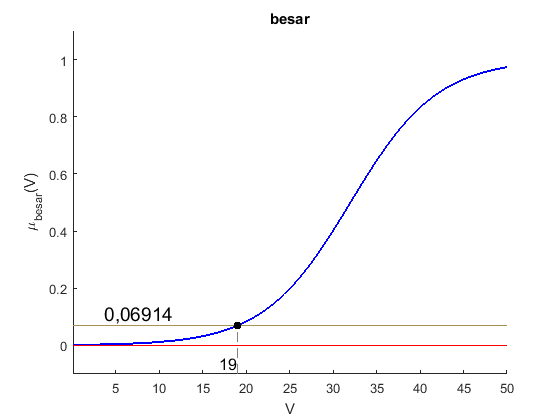
\includegraphics[width=3.1cm]{V_besar} & 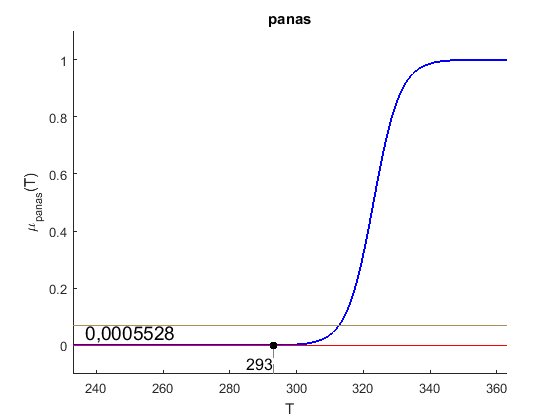
\includegraphics[width=3.1cm]{T_panas} &
    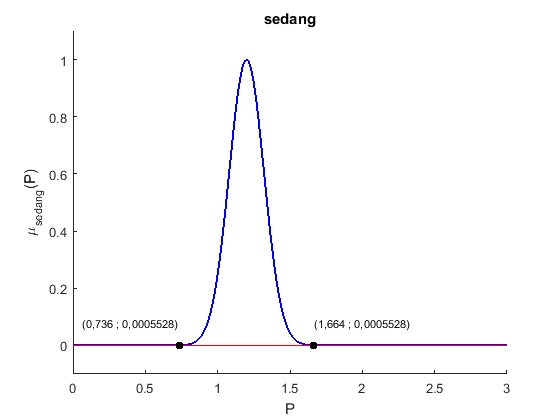
\includegraphics[width=3.1cm]{P_sedang} & 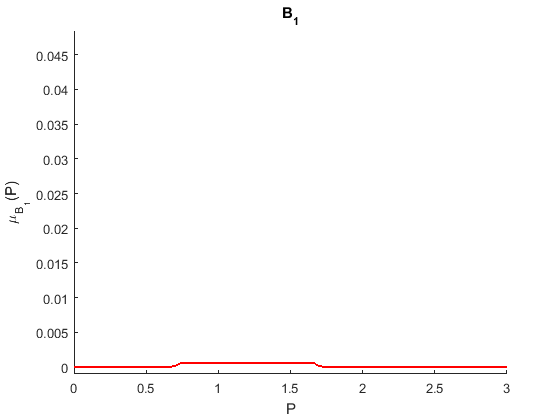
\includegraphics[width=3.1cm]{B1} \\
    Kecil & Normal & Tinggi & $\text{B}_2$\\
    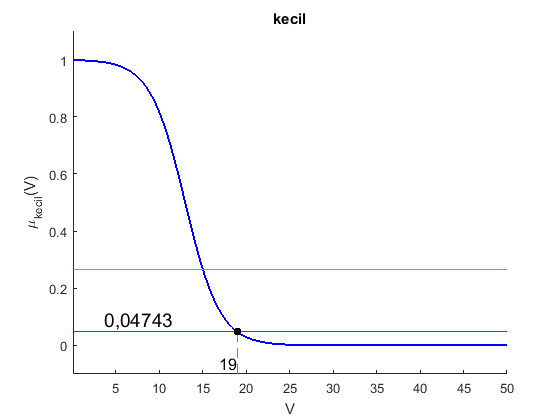
\includegraphics[width=3.1cm]{V_kecil} & 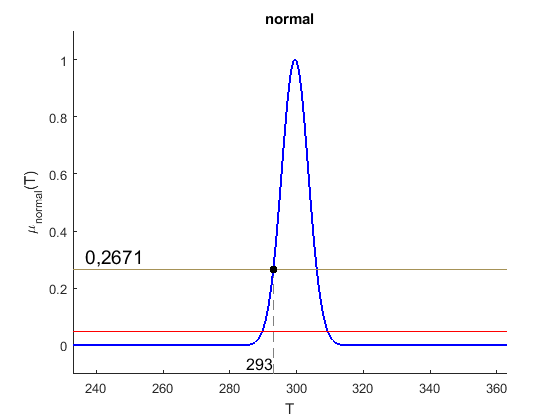
\includegraphics[width=3.1cm]{T_normal} &
    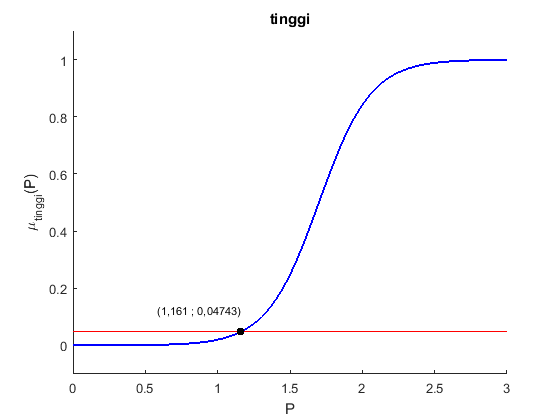
\includegraphics[width=3.1cm]{P_tinggi} & 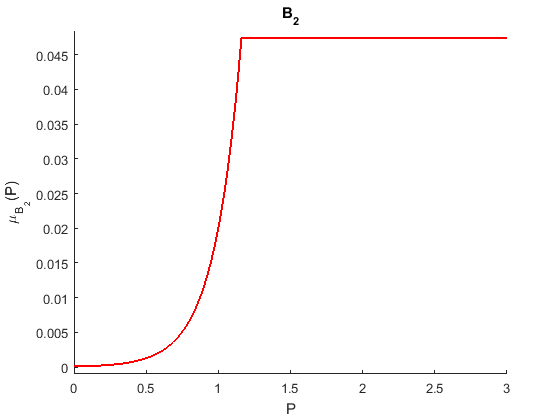
\includegraphics[width=3.1cm]{B2} \\
    Standar & Dingin & Rendah & $\text{B}_3$\\
    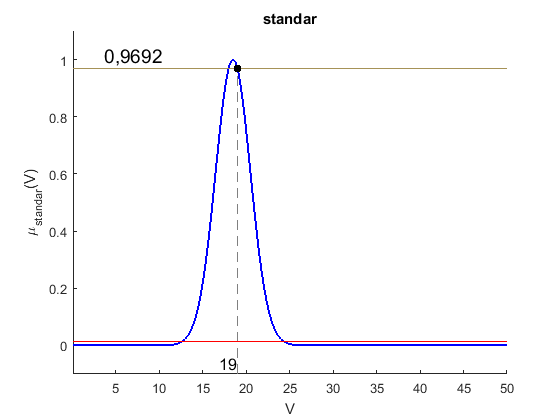
\includegraphics[width=3.1cm]{V_standar} & 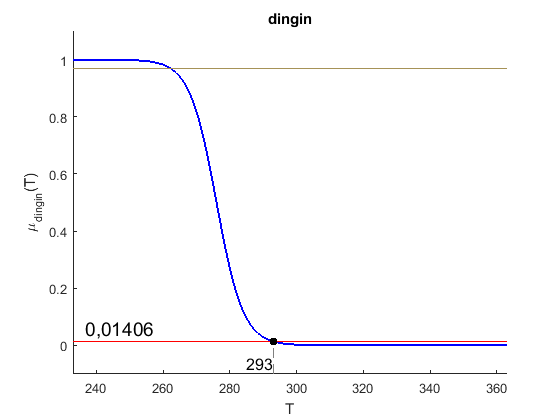
\includegraphics[width=3.1cm]{T_dingin} &
    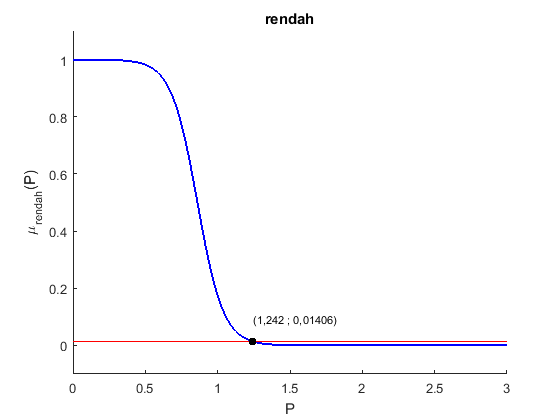
\includegraphics[width=3.1cm]{P_rendah} & 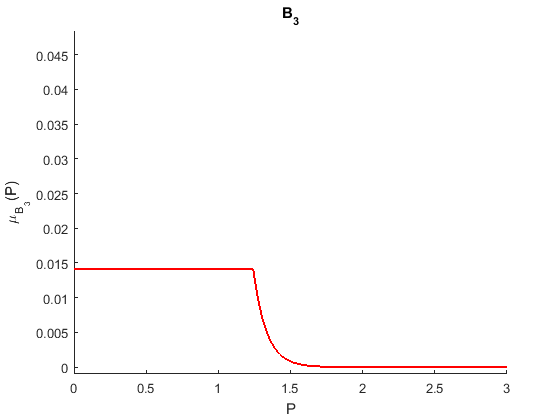
\includegraphics[width=3.1cm]{B3} \\
    \midrule
    \multicolumn{2}{c}{Penggabungan aturan fuzzy} & \multicolumn{2}{c}{Hasil akhir}\\
    \multicolumn{2}{c}{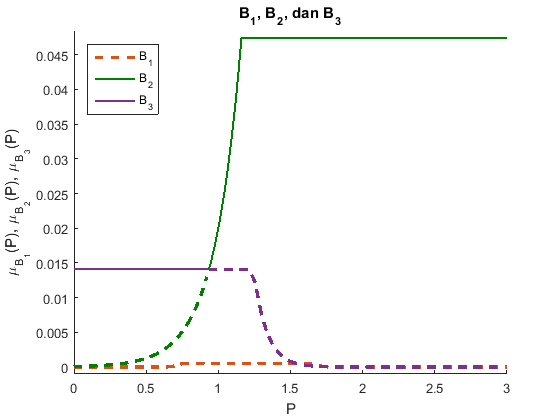
\includegraphics[width=5.8cm]{B}} & \multicolumn{2}{c}{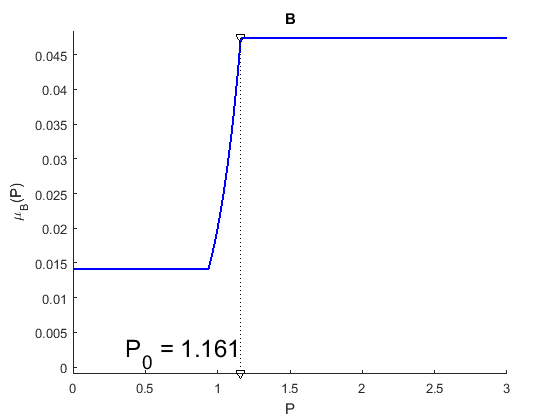
\includegraphics[width=5.8cm]{hasilB}}\\
    \bottomrule
    \end{tabular}
\end{table}
\noindent Misalkan digunakan operator minimum untuk \emph{t-norm} dan operator maksimum untuk \emph{t-conorm}. Inferensi mamdani untuk menyelesaikan SKLF ini dapat dilihat pada \ref{tab:inferensi mamdani}. Lakukan fuzzifikasi terhadap serangkaian fakta dan operasi \emph{t-norm} bagian pendahulu untuk setiap implikasi, sehingga diperoleh
\begin{align*}
    \mu_{besar}(19) &= \num{0,0691}, & \mu_{panas}(293) &= \num{0,0006}, &\text{maka } \alpha_1&= \num{0,0006},\\
    \mu_{kecil}(19) &= \num{0,0474}, & \mu_{normal}(293) &= \num{0,2671},&\text{maka } \alpha_2&= \num{0,0474},\\
    \mu_{standar}(19) &= \num{0,9692}, & \mu_{dingin}(293)&= \num{0,0141},&\text{maka } \alpha_3&= \num{0,0141}
\end{align*}
Selanjutnya operasikan bagian pendahulu di atas dengan nilai linguistik dari variabel kontrol dengan menggunakan operator implikasi Mamdani. Akibatnya, diperoleh tiga himpunan fuzzy baru di $\mathbb{R}^+$, yaitu himpunan fuzzy $B_1$, $B_2$, dan $B_3$. Untuk setiap $P \in \mathbb{R}^+$, fungsi keanggotaan himpunan fuzzy $B_1$, $B_2$, dan $B_3$ adalah
\begingroup
\allowdisplaybreaks
\begin{align*}
\begin{split}
    \mu_{B_1}(P) &= \min \{\alpha_1, \mu_{sedang}(P) \}
    = \min \left\{ \num{0,0006} \text{, } \mu_{sedang}(P) \right\}\\
    &=
    \begin{dcases}
    \num{0,0006}, & \num{0,736} \leq P \leq \num{1,664} \\
    \exp \left[-\displaystyle\frac{1}{2} \left( \displaystyle\frac{P-\num{1,2}}{\num{0,12}} \right)^2 \right], & \text{lainnya}
    \end{dcases}
\end{split}\\
\begin{split}
    \mu_{B_2}(P) &= \min \{\alpha_2, \mu_{tinggi}(P) \}
    = \min \left\{ \num{0,0474} \text{, } \mu_{tinggi}(P)  \right\}\\
    & =
    \begin{dcases}
    \displaystyle\frac{1}{ 1+\exp\left(\displaystyle\frac{\num{1,7}-P}{\num{0,18}} \right) }, & P < \num{1,161}\\
    \num{0,0474}, & \text{lainnya}
    \end{dcases}
\end{split}\\
\begin{split}
    \mu_{B_3}(P) &= \min \{\alpha_3, \mu_{rendah}(P) \}
    = \min \left\{ \num{0,0141} \text{, } \mu_{rendah}(P) \right\}\\
    & =
    \begin{dcases}
    \displaystyle\frac{1}{ 1+\exp\left(\displaystyle\frac{P-\num{0,86}}{\num{0,09}} \right) }, & P \geq \num{1,242}\\
    \num{0,0141}, & \text{lainnya}
    \end{dcases}
\end{split}
\end{align*}
\endgroup

Gabungkan himpunan fuzzy $B_1$, $B_2$, dan $B_3$ menggunakan operasi \emph{t-conorm}. Maka diperoleh himpunan fuzzy $B$ di $\mathbb{R}^+$ dengan fungsi keanggotaan
\begin{align*}
    \mu_B(P) &= \maks \left\{ \mu_{B_1}(P),\mu_{B_2}(P),\mu_{B_3}(P) \right\}\\
    &=
    \begin{dcases}
    \num{0,0141}, & P < \num{1,242}\\
    \frac{1}{ 1+\exp\left(\frac{\num{1,7}-P}{\num{0,18}} \right) }, & \num{1,242} \leq P < \num{1,161}\\
    \num{0,0474}, & P \geq \num{1,161}
    \end{dcases}
\end{align*}
Misalkan operator defuzzifikasi yang digunakan adalah \emph{first-of-maxima}. Maka diperoleh
\begin{align*}
    P_0 &= \min \left\{P \in \mathbb{R}^+ : \mu_B(P) = \underset{w}{\maks}\mu_B(w) = \num{0,0474}  \right\}\\
    &= \min \left\{ P \in \mathbb{R}^+ : P \geq \num{1,161}\right\}\\
    &= \num{1,161}
\end{align*}
Dengan demikian, tindakan kontrol dari SKLF ini adalah $P_0 = \num{1,161}$. Artinya, ketika volume suatu gas ideal sebesar 19 liter dan suhunya bernilai 293 Kelvin, maka berdasarkan aturan fuzzy ini dan mekanisme inferensi mamdani, diperoleh tekanan sebesar $\num{1,161} \text{ } atm$.
\end{contoh}

\subsubsection{Mekanisme Inferensi Takagi-Sugeno-Kang}
\noindent Inferensi TSK merupakan inferensi fuzzy yang dilakukan terhadap aturan fuzzy TSK. Pada dasarnya, mekanisme inferensi TSK sama seperti mekanisme inferensi Mamdani. Operator implikasi menggunakan operator Mamdani, dan menggunakan ``atau'' sebagai penghubung antar implikasi. Tetapi, inferensi TSK memiliki kasus khusus berupa nilai linguistik variabel kontrol yang diskrit dan menyerupai pendefinisian himpunan klasik, sebagaimana telah diformulasikan pada Persamaan (\ref{TSK kontrol}). Selain itu, metode defuzzifikasi yang digunakan pada SKLF ini hanya metode \emph{center-of-area} karena himpunan fuzzy yang dihasilkan dari inferensi ini merupakan himpunan fuzzy diskrit.

\noindent Misalkan diberikan himpunan fuzzy $A_{1,j},A_{2,j}, \ldots, A_{m,j}$  di $X_j$ dengan $j=1,2,\ldots,n$, $\mathbf{b}_i = (b_{i,0},b_{i,1},\ldots, b_{i,n})$ dengan $i=1,2,\ldots,m$, dan $\mathbf{\Tilde{x}} = (1,x_1,x_2,\ldots,x_n)$. Asumsikan $\mathbf{b}_i \neq \mathbf{b}_k$ untuk setiap $i\neq k$. Kemudian diberikan SKLF berikut ini
\flctsk
Pandang bagian konsekuensi dari setiap implikasi di atas sebagai ``$y$ adalah $B_i$'' untuk setiap $i=1,2,\ldots,m$ dengan fungsi keanggotaan $\mu_{B_i}$ sama seperti fungsi keanggotaan pada (\ref{TSK kontrol}). Karena terdapat serangkaian fakta $x_1=a_1, x_2=a_2, \ldots, x_n=a_n$, maka fungsi keanggotaan $\mu_{B_i}$ menjadi
\[\mu_{B_i} = 
\begin{dcases}
1, & \text{jika } y=\mathbf{b}_i\cdot\mathbf{\Tilde{a}}, \quad \mathbf{\Tilde{a}} = (1,a_1,a_2,\ldots,a_n)\\
0, & \text{lainnya}
\end{dcases}
\]
\noindent Langkah-langkah untuk mendapatkan nilai $y_0$ sebagai tindakan kontrol dari SKLF ini sama seperti langkah-langkah pada inferensi Mamdani. Perbedaannya terletak pada kasus khusus yang ada di variabel kontrol. Rincian langkah-langkahnya adalah sebagai berikut
\begin{enumerate}
    \item Lakukan fuzzifikasi terhadap serangkaian fakta berdasarkan nilai linguistik dari variabel kondisi. Kemudian operasikan hasil fuzzifikasi tersebut dengan operasi konjungsi fuzzy (\emph{t-norm}). Misalkan hasil operasi ini dinyatakan dengan $\alpha_i$ untuk $i=1,2,\ldots m$. Maka diperoleh
    \[\alpha_i = T\left( \mu_{A_{i,1}}(a_1),\mu_{A_{i,2}}(a_2),\ldots,\mu_{A_{i,n}}(a_n) \right)
    \text{,} \quad i = 1,2,\ldots,m
    \]
    \item Operasikan bagian pendahulu dan bagian konsekuensi pada setiap implikasi menggunakan operator mamdani. Maka diperoleh sebanyak $m$ himpunan fuzzy baru di $Y$, yaitu himpunan fuzzy $B'_1, B'_2, \ldots, B'_m$ dengan fungsi keanggotaan
    \begin{align*}
        \mu_{B'_i}(y) &= \min \left\{ \alpha_i, \mu_{B_i}(y) \right\}\text{,} \quad y \in Y \quad i = 1,2,\ldots,m\\
        &=
        \begin{dcases}
        \min \left\{ \alpha_i, 1 \right\} = \alpha_i \text{,} & y = \mathbf{b}_i\cdot\mathbf{\Tilde{a}}\\
        \min \left\{ \alpha_i, 0 \right\} = 0 \text{,} & y \text{ lainnya}
        \end{dcases}
    \end{align*}
    \item Selanjutnya, dilakukan operasi \emph{t-conorm} untuk menggabungkan sebanyak $m$ himpunan fuzzy dari setiap implikasi. Maka diperoleh himpunan fuzzy baru di $Y$, yaitu himpunan fuzzy $B$ dengan fungsi keanggotaan
    \[ \mu_B(y) = S\left(\mu_{B'_1}(y),\mu_{B'_2}(y),\ldots,\mu_{B'_m}(y)\right) \text{,} \quad y \in Y \]
    Karena untuk setiap $i=1,2,\ldots,m$ $\mu_{B'_i}(y) = \alpha_i$ hanya dipenuhi oleh $y= \mathbf{b}_i\cdot\mathbf{\Tilde{a}}$ dan $\mu_{B'_i}(y) = 0$ untuk $y$ yang lain, maka
    \begin{align*}
        \displaystyle \mu_B(y) &= 
        \begin{dcases}
        S\left(\alpha_1,0,\ldots,0\right) = \alpha_1\text{,} & y = \mathbf{b}_1\cdot\mathbf{\Tilde{a}}\\
        \vdots &\vdots\\
        S\left(0,0,\ldots,\alpha_i,\ldots,0,0\right) = \alpha_i\text{,} & y = \mathbf{b}_i\cdot\mathbf{\Tilde{a}}\\
        \vdots &\vdots\\
        S\left(0,0,\ldots,0,\alpha_m\right) = \alpha_m\text{,} & y = \mathbf{b}_m\cdot\mathbf{\Tilde{a}}\\
        0\text{,} &y \text{ lainnya}
        \end{dcases}
    \end{align*}
    Dengan demikian, $B$ merupakan himpunan fuzzy diskrit.
    \item Langkah terakhir, lakukan defuzzifikasi menggunakan metode \emph{center-of-area} terhadap himpunan fuzzy $B$ untuk mendapatkan nilai dari tindakan kontrol $y_0$, sehingga diperoleh
    \[ y_0 = \displaystyle \frac{\displaystyle\sum_{y \in Y} \mu_B(y)y}{\displaystyle\sum_{y \in Y} \mu_B(y)} \]
    Misalkan $y_i = \mathbf{b}_i\cdot\mathbf{\Tilde{a}}$ untuk setiap $i=1,2,\ldots,m$. Maka $\mu_B(y)>0$ hanya berlaku untuk $y \in \{y_1,y_2,\ldots,y_m\}$. Dengan demikian, diperoleh
    \begin{align*}
        y_0 &= \displaystyle \frac{\displaystyle\sum_{i=1}^m \mu_B(y_i)y_i}{\displaystyle\sum_{i=1}^m \mu_B(y_i)}
         = \displaystyle \frac{\displaystyle\sum_{i=1}^m \alpha_i y_i}{\displaystyle\sum_{i=1}^m \alpha_i}
    \end{align*}
\end{enumerate}

\noindent Contoh \ref{contoh: inf tsk} berikut ini memberikan gambaran tambahan mengenai mekanisme inferensi TSK.

\begin{contoh} \label{contoh: inf tsk}
Misalkan diberikan sistem gas ideal yang terdiri dari volume ($V$) dengan satuan $liter$, suhu ($T$) dengan satuan $Kelvin$, dan tekanan ($P$) dengan satuan $atm$. Sistem gas ideal ini dapat dipandang sebagai SKLF dengan $V$ dan $T$ sebagai variabel kondisi dan $P$ adalah variabel kontrolnya. Misalkan
\begin{itemize}
    \item Variabel kondisi $V$ memiliki tiga nilai linguistik: besar, standar, dan kecil. Fungsi keanggotaan dari tiga nilai linguistik ini didefinisikan pada Contoh \ref{contoh inf mamdani}.
    \item Variabel kondisi $T$ memiliki tiga nilai linguistik: panas, normal, dan dingin dengan fungsi keanggotaan didefinisikan pada Contoh \ref{contoh inf mamdani}.
\end{itemize}

Misalkan SKLF tersebut adalah sebagai berikut
\begin{align*}
\Re_1 &: \text{ Jika} && V \text{ besar,} && T \text{ panas,}&&\text{maka}&&P&&= \num{1,181} - \num{0,045}V\\
 & && && && && && + \num{0,003}T\\
\Re_2 &: \text{ Jika} && V \text{ kecil,} && T \text{ normal,}&&\text{maka}&&P&&= \num{2,3312} + \num{0,0711}V\\
 & && && && && && - \num{0,003}T\\
\Re_3 &: \text{ Jika} && V \text{ standar,} && T \text{ dingin,}&&\text{maka}&&P&&= \num{21,71} - \num{0,05}V\\
 & && && && && && - \num{0,07}T\\
\text{Fakta} &: && V = 19\text{,} && T = 293\\
\hline
\text{Konklusi} &: && && && && P &&= P_0
\end{align*}

\noindent Misalkan digunakan operator minimum untuk \emph{t-norm}. Lakukan fuzzifikasi terhadap serangkaian fakta dan operasi \emph{t-norm} bagian pendahulu untuk setiap implikasi, sehingga diperoleh
\begin{align*}
    \mu_{besar}(19) &= \num{0,0691}, & \mu_{panas}(293) &= \num{0,0006}, &\text{maka } \alpha_1&= \num{0,0006},\\
    \mu_{kecil}(19) &= \num{0,0474}, & \mu_{normal}(293) &= \num{0,2671},&\text{maka } \alpha_2&= \num{0,0474},\\
    \mu_{standar}(19) &= \num{0,9692}, & \mu_{dingin}(293)&= \num{0,0141},&\text{maka } \alpha_3&= \num{0,0141}
\end{align*}
Selanjutnya, tentukan nilai $P_1$, $P_2$, dan $P_3$ berdasarkan serangkaian fakta dan variabel kontrol $P$ pada setiap konsekuensi.
\begin{center}
    \begin{tabular}{rll}
        $P_1$ &= $\num{1,181} - \num{0,045}(19) + \num{0,003}(293)$ &= $\num{1,205}$\\
        $P_2$ &= $\num{2,3312} + \num{0,0711}(19) - \num{0,003}(293)$ &= $\num{2,8031}$\\
        $P_3$ &= $\num{21,71} - \num{0,05}(19)  - \num{0,07}(293)$ &= $\num{0,25}$
    \end{tabular}\\
\end{center}
Dengan demikian, diperoleh tindakan kontrol $P_0$, yaitu
\begin{align*}
    P_0 = \displaystyle \frac{\displaystyle\sum_{i=1}^3 \alpha_i P_i}{\displaystyle\sum_{i=1}^3 \alpha_i}
    = \displaystyle \frac{\num{0,0006}(\num{1,205})+\num{0,0474}(\num{2,8031}) + \num{0,0141}(\num{0,25})}{\num{0,0006}+\num{0,0474} + \num{0,0141}}
    = \num{2,2079}
\end{align*}
\end{contoh}

%%%%-----KONSTRUKSI JARINGAN SARAF FUZZY------
\section{Konstruksi Jaringan Saraf Fuzzy} \label{konst fnn}
\noindent Aturan fuzzy yang terdapat pada SKLF yang dibahas pada Subbab \ref{flc} berasal dari pengetahuan para ahli. Pada subbab ini akan dipelajari cara membangun aturan fuzzy yang bukan berasal dari pengetahuan para ahli, melainkan berdasarkan data masukan dan keluaran yang diberikan. Aturan fuzzy yang akan dibangun hanya terbatas pada aturan fuzzy TSK. Fungsi keanggotaan dari nilai linguistik variabel kondisi hanya menggunakan fungsi Gauss, yaitu
\begin{align} \label{gauss}
    g(x; m,s) = \displaystyle \exp \left[ -\displaystyle \frac{1}{2}\left( \displaystyle \frac{x-m}{s} \right)^2 \right]
\end{align}
dengan $m$ dan $s$ merupakan parameter tertentu yang akan dicari.

\noindent Misalkan diberikan variabel kondisi $x_1,x_2,\ldots,x_n$. Untuk setiap variabel kondisi $x_j$ memiliki nilai linguistik berupa himpunan fuzzy $A_{1,j},A_{2,j},\ldots,A_{r,j}$ di $X_j$ dengan $j=1,2,\ldots,n$. Setiap himpunan fuzzy $A_{i,j}$ memiliki fungsi keanggotaan berupa fungsi Gauss, yaitu
\[\mu_{A_{i,j}}(x_j) = g(x_j; m_{i,j}, s_{i,j})\]
Untuk menyingkat penulisan notasi, derajat keanggotaan $x_j$ di himpunan fuzzy $A_{i,j}$ dinyatakan sebagai $G_{i,j}$, dengan kata lain $G_{i,j} = \mu_{A_{i,j}}(x_j)$. Fungsi $g$ didefinisikan pada Persamaan (\ref{gauss}). Selanjutnya, diberikan variabel kontrol $y_1,y_2,\ldots,y_p$. Variabel-variabel kontrol ini dapat ditulis ke dalam bentuk vektor menjadi 
\[\mathbf{y} = (y_1,y_2,\ldots,y_p)\]
Untuk setiap implikasi ke-$i$, entri di dalam vektor variabel kontrol ini ditentukan oleh $\mathbf{y}^{\text{ }T} = \mathbf{B}_i\mathbf{\Tilde{x}}^{\text{ }T}$ dengan $i=1,2,\ldots,r$ dan
\begin{align}
\label{matriks Bi}
\mathbf{B}_i &=
\begin{bmatrix}
b_{i,1,0} & b_{i,1,1} & b_{i,1,2} & \dots & b_{i,1,n} \\
b_{i,2,0} & b_{i,2,1} & b_{i,2,2} & \dots & b_{i,2,n} \\
\vdots & \vdots & \vdots & & \vdots \\
b_{i,p,0} & b_{i,p,1} & b_{i,p,2} & \dots & b_{i,p,n}
\end{bmatrix}
=
\begin{bmatrix}
\mathbf{b}_{i,1} \\
\mathbf{b}_{i,2} \\
\vdots \\
\mathbf{b}_{i,p}
\end{bmatrix}
\\
\mathbf{\Tilde{x}} &= (1,x_1,x_2,\ldots,x_n) \nonumber
\end{align}
Kemudian diberikan serangkaian fakta $x_1=c_1,x_2=c_2,\ldots,x_n=c_n$ dan konklusi yang berupa tindakan kontrol $\mathbf{y} = \mathbf{d} = (d_1,d_2,\ldots,d_p)$. Setiap fakta $c_j$ dengan $j=1, 2,\ldots,n$ berasal dari data masukan pada suatu observasi dan setiap tindakan kontrol $d_k$ dengan $k=1, 2, \ldots, p$ berasal dari data keluaran pada observasi tersebut. Berdasarkan premis-premis ini, diperoleh SKLF berikut
\begin{equation} \label{SKLF FNN}
    \begin{aligned}
    \Re_1 &: \text{ Jika } &&x_1 \text{ anggota } A_{1,1} \text{,} &&\ldots \text{,} &&x_n \text{ anggota } A_{1,n} \text{,}
    &&\text{maka } &&\mathbf{y}^{\text{ }T} = \mathbf{B}_1\mathbf{\Tilde{x}}^{\text{ }T}\\
    \Re_2 &: \text{ Jika } &&x_1 \text{ anggota } A_{2,1} \text{,} &&\ldots \text{,} &&x_n \text{ anggota } A_{2,n} \text{,}
    &&\text{maka } &&\mathbf{y}^{\text{ }T} = \mathbf{B}_2\mathbf{\Tilde{x}}^{\text{ }T}\\
    & && &&\vdots \\
    \Re_r &: \text{ Jika } &&x_1 \text{ anggota } A_{r,1} \text{,} &&\ldots \text{,} &&x_n \text{ anggota } A_{r,n} \text{,}
    &&\text{maka } &&\mathbf{y}^{\text{ }T} = \mathbf{B}_r\mathbf{\Tilde{x}}^{\text{ }T}\\
    \text{Fakta} &: &&x_1 = c_1 \text{,} &&\ldots \text{,} &&x_n = c_n \\
    \hline
    \text{Konklusi} &: && && && && &&\mathbf{y} = \mathbf{d}
    \end{aligned}
\end{equation}
SKLF pada (\ref{SKLF FNN}) dapat diilustrasikan sebagai suatu jaringan saraf yang dapat dilihat pada \ref{fig:jsf}. Jaringan saraf ini disebut dengan jaringan saraf fuzzy (JSF). Hal ini dikarenakan jaringan tersebut dibangun dari aturan fuzzy dan penentuan nilai dari neuron-neuronnya berdasarkan tahapan-tahapan pada SKLF.

\begin{figure}[t!]
    \centering
    \begin{tikzpicture} [thick,scale=0.89, every node/.style={scale=1}]
    \small
    %neurons
    %input layer
    \bulat[as,(-1,1.5)] {$c_1$};\bulat[aj,(-1,0)] {$c_j$}; \bulat[an,(-1,-1.5)] {$c_n$};
    %fuzzifikasi
    \bulat[gss,(4,6.5)]{$G_{1,1}$}; \bulat[gsj,(4,5)]{$G_{1,j}$}; \bulat[gsn,(4,3.5)]{$G_{1,n}$};
    \bulat[gis,(4,1.5)]{$G_{i,1}$}; \bulat[gij,(4,0)]{$G_{i,j}$}; \bulat[gin,(4,-1.5)]{$G_{i,n}$};
    \bulat[grs,(4,-3.5)]{$G_{r,1}$}; \bulat[grj,(4,-5)]{$G_{r,j}$}; \bulat[grn,(4,-6.5)]{$G_{r,n}$};
    %t-norm
    \bulat[aas,(8,2)]{$\alpha_1$}; \bulat[aai,(8,0)]{$\alpha_i$}; \bulat[aar,(8,-2)]{$\alpha_r$};
     %output layer
    \bulat[ts,(10,1.6)] {$t_1$}; \bulat[tk,(10,0)] {$t_k$}; \bulat[tp,(10,-1.6)] {$t_p$};
     
     %dots
     \titiks[as,aj]; \titiks[aj,an];
     \titiks[gss,gsj]; \titiks[gsj,gsn]; \titiks[gis,gij]; \titiks[gij,gin]; \titiks[grs,grj]; \titiks[grj,grn];
     \titikb[gsn,gis]; \titikb[gin,grs];
     \titiks[aas,aai]; \titiks[aai,aar];
     \titiks[ts,tk]; \titiks[tk,tp];
     
    %Lines
    %input to fuzzification
    \singleT[as,gss,0,above]{$(m_{1,1},s_{1,1})$}; \singleT[aj,gsj,0,above]{}; \singleT[an,gsn,0,above]{};
    \singleT[as,gis,0,above]{}; \singleT[aj,gij,0,above]{$(m_{i,j},s_{i,j})$}; \singleT[an,gin,0,above]{};
    \singleT[as,grs,0,above]{}; \singleT[aj,grj,0,above]{}; \singleT[an,grn,0,below]{$(m_{r,n},s_{r,n})$};
    %f to t-norm
    \singleT[gss,aas,0,above]{}; \singleT[gsj,aas,0,above]{}; \singleT[gsn,aas,0,above]{};
    \singleT[gis,aai,0,above]{}; \singleT[gij,aai,0,above]{}; \singleT[gin,aai,0,above]{};
    \singleT[grs,aar,0,above]{}; \singleT[grj,aar,0,above]{}; \singleT[grn,aar,0,above]{};
    %t-norm to output
    \singleT[aas,ts,0,above]{$\mathbf{b}_{1,1}\cdot\mathbf{\Dot{c}}$}; \singleT[aai,ts,0,above]{}; \singleT[aar,ts,0,above]{};
    \singleT[aas,tk,0,above]{}; \singleT[aai,tk,0,above]{}; \singleT[aar,tk,0,above]{};
    \singleT[aas,tp,0,above]{}; \singleT[aai,tp,0,above]{}; \singleT[aar,tp,0,below]{$\mathbf{b}_{r,p}\cdot\mathbf{\Dot{c}}$};
    \end{tikzpicture}
    \caption{Jaringan saraf fuzzy}
    \label{fig:jsf}
\end{figure}

\noindent JSF untuk kasus ini terdiri dari lapisan masukan, dua lapisan tersembunyi, dan lapisan keluaran. Neuron pada lapisan masukan diperoleh dari serangkaian fakta pada SKLF (\ref{SKLF FNN}). Neuron pada lapisan tersembunyi pertama adalah hasil dari fuzzifikasi dari neuron pada lapisan masukan. Neuron pada lapisan tersembunyi kedua merupakan hasil operasi \emph{t-norm} dari blok-blok neuron pada lapisan tersembunyi pertama. Penentuan blok ini berdasarkan aturan fuzzy pada SKLF (\ref{SKLF FNN}). Pada jaringan saraf fuzzy, operator \emph{t-norm} yang digunakan adalah operator probabilistik (perkalian). Maka nilai dari neuron-neuron pada lapisan tersembunyi kedua adalah
\begin{align*}
    \alpha_i &= \displaystyle \prod_{j=1}^n G_{i,j} = \displaystyle \prod_{j=1}^n g(c_j; m_{i,j}, s_{i,j})
    = \displaystyle \prod_{j=1}^n \displaystyle \exp \left[ \displaystyle -\frac{1}{2}\left( \displaystyle \frac{c_j-m_{i,j}}{s_{i,j}} \right)^2 \right] \\
    &= \displaystyle \exp \left[ -\displaystyle \frac{1}{2} \displaystyle\sum_{j=1}^n \left( \displaystyle \frac{c_j-m_{i,j}}{s_{i,j}} \right)^2 \right],
    \quad i=1,2,\ldots,r
\end{align*}
Neuron pada lapisan keluaran merupakan tindakan kontrol aktual yang dinyatakan dengan $\mathbf{t} = (t_1,t_2,\ldots,t_p)$, yaitu
\[ \mathbf{t}^{\text{  }T} = \displaystyle \frac{\displaystyle \sum_{i=1}^r \alpha_i \mathbf{B_i} \mathbf{\Tilde{c}}^{\text{  }T} }{\displaystyle \sum_{i=1}^r \alpha_i } \]
dengan $\mathbf{\Tilde{c}} = (1,c_1,c_2,\ldots,c_n)$ dan matriks $\mathbf{B}_i$ didefinisikan pada (\ref{matriks Bi}). Tindakan kontrol aktual $\mathbf{t}$ tidak sama dengan tindakan kontrol yang diinginkan pada SKLF \ref{SKLF FNN} ($\mathbf{d}$). Tetapi, $\mathbf{t}$ yang diperoleh harus sangat dekat dengan $\mathbf{d}$.

\noindent Berdasarkan penjelasan di atas, entri pada vektor $\mathbf{t}$ ditentukan dari proses \emph{feedforward} pada JSF. Proses \emph{feedforward} ini analog dengan seluruh tahapan pada SKLF, yaitu: fuzzifikasi, inferensi, dan defuzzifikasi. Nilai neuron-neuron pada lapisan tersembunyi pertama bergantung kepada nilai dari parameter $m_{i,j}$ dan $s_{i,j}$ dengan $i=1,2,\ldots,r$ dan $j=1,2,\ldots,n$. Nilai neuron-neuron pada lapisan tersembunyi kedua tidak dipengaruhi oleh parameter apapun karena hanya dilakukan operasi \emph{t-norm}. Nilai $\mathbf{t}$ sangat dipengaruhi oleh parameter $b_{i,k,0}$ dan $b_{i,k,j}$ dengan $i=1,2,\ldots,r$, $k=1,2,\ldots,p$ dan $j=1,2,\ldots,n$. Dengan demikian, target utama dari konstruksi JSF adalah menentukan nilai dari parameter-parameter $m_{i,j}$, $s_{i,j}$, $b_{i,k,0}$, dan $b_{i,k,j}$ sedemikian sehingga dapat meminimalkan rataan galat kuadrat atau \emph{mean square error} (\gls{mse}) antara tindakan kontrol aktual ($t_1, t_2, \ldots, t_p$) dan tindakan kontrol yang diinginkan ($d_1, d_2, \ldots, d_p$).\\

\begin{figure}[htbp!]
    \centering
    \begin{tikzpicture}
    \node (awal)   at (0,0)    {};
    \kotaktl[is,(4,0)]{Identifikasi}{Struktur};
    \kotaktl[ip,(9,0)]{Identifikasi}{Parameter};
    \node (akhir)   at (12.5,0)    {};
    
    \singleTf[awal,is,0,above,9]{Data berukuran $L\times(n+p)$};
    \singleTf[is,ip,0,above,9]{Struktur awal aturan fuzzy};
    \singleTf[ip,akhir,0,above,9]{Struktur akhir aturan fuzzy};
    \end{tikzpicture}
    \caption{Dua fase pada konstruksi jaringan saraf fuzzy}
    \label{fig:dua fase}
\end{figure}

\noindent Misalkan diberikan data dengan observasi sebanyak $L$. Misalkan setiap observasi memiliki sebanyak $n$ masukan dan $p$ keluaran, sehingga setiap observasi dapat dipandang sebagai vektor masukan dengan dimensi $n$ dan vektor keluaran dengan dimensi $p$. Maka dapat dikatakan bahwa data ini memiliki ukuran sebesar $L\times(n+p)$. Menurut \citeasnoun{lee} dan \citeasnoun{yeh}, konstruksi JSF berdasarkan data ini harus melalui dua fase, yaitu: identifikasi struktur dan identifikasi parameter. Fase identifikasi struktur dilakukan untuk memperoleh struktur awal dari aturan fuzzy. Struktur awal ini meliputi banyaknya implikasi pada aturan fuzzy dan inisialisasi nilai dari setiap parameter. Fase identifikasi parameter dilakukan untuk memperbaiki nilai dari parameter-parameter $m_{i,j}$, $s_{i,j}$, $b_{i,k,0}$, dan $b_{i,k,j}$ sedemikian sehingga target utama dari konstruksi JSF tercapai. Dua fase ini telah diringkas di dalam \ref{fig:dua fase}.

\subsection{Identifikasi Struktur}
\noindent Pada fase ini, terdapat dua tahap utama. Pertama, pengelompokan data ke dalam klaster menggunakan algoritma \emph{self-constructing clustering}. Tahap pertama ini akan menghasilkan klaster-klaster dari data yang diberikan. Setiap Klaster ke-$i$ memiliki parameter $\mathbf{m}_i=(m_{i,1}, m_{i,2}, \ldots, m_{i,n})$ dan $\mathbf{s}_i=(s_{i,1}, s_{i,2}, \ldots, s_{i,n})$. Parameter $\mathbf{m}_i$ dan $\mathbf{s}_i$, berturut-turut, adalah vektor rata-rata dan vektor simpangan baku dari vektor data masukan yang ada di klaster ke-$i$. Nantinya, setiap parameter $m_{i,j}$ dan $s_{i,j}$ yang diperoleh dari tahap ini menjadi nilai awal dari parameter untuk fungsi Gauss yang bersesuaian. Oleh karena itu, kaitannya dengan JSF dan SKLF, setiap klaster dapat dipandang sebagai satu implikasi pada aturan fuzzy. Selanjutnya, tahap kedua adalah menentukan nilai dari parameter pada variabel kontrol, yaitu entri dari setiap matriks $\mathbf{B}_i$, menggunakan metode dekomposisi nilai singular.

\subsubsection{\emph{Self-constructing Clustering}}
\noindent Asumsikan data yang akan diolah berukuran $L\times(n+p)$. Setiap observasi ke-$l$ dalam data ini memiliki pola $[\mathbf{c}^{(l)}, \mathbf{d}^{(l)}]$, dengan
\[\mathbf{c}^{(l)} = (c_1^{(l)},c_2^{(l)},\ldots,c_n^{(l)})\]
menyatakan $n$ nilai data masukan pada observasi ke-$l$ dan
\[\mathbf{d}^{(l)} = (d_1^{(l)},d_2^{(l)},\ldots,d_p^{(l)})\]
menyatakan $p$ nilai data keluaran pada observasi ke-$l$.

\noindent Sebagaimana telah dijelaskan sebelumnya, algoritma \emph{self-constructing clustering} mengelompokkan masing-masing observasi dari data ke dalam klaster. Pengelompokan ini berdasarkan uji kemiripan data masukan dan uji kemiripan data keluaran. Setiap klaster memuat beberapa observasi tertentu dari data. Setiap klaster dikarakterisasi oleh hasil operasi \emph{t-norm} dari fungsi keanggotaan nilai linguistik dari variabel kondisi. Karena fungsi keanggotaan yang digunakan adalah fungsi Gauss dan operator \emph{t-norm} yang digunakan adalah perkalian, maka setiap klaster dikarakterisasi oleh hasil kali dari sebanyak $n$ fungsi Gauss. Selain itu, setiap klaster juga memiliki vektor ketinggian, yaitu vektor rata-rata dari data keluaran yang ada di dalam klaster tersebut \cite{yeh}.

\noindent Dalam \emph{self-constructing clustering}, setiap observasi dari data diperiksa satu per satu. Pada awalnya, observasi pertama dimasukkan ke dalam klaster pertama. Untuk setiap observasi berikutnya, diuji kemiripan data masukan dan kemiripan data keluaran antara observasi tersebut dengan klaster-klaster yang telah ada. Pengujian kemiripan ini akan memutuskan apakah observasi tersebut dimasukkan ke dalam klaster tertentu yang telah ada atau observasi tersebut menjadi anggota pertama pada klaster yang baru. Setelah semua observasi diperiksa, akan diperoleh banyaknya klaster yang terbentuk. Rincian dari \emph{self-constructing clustering} akan dijelaskan di bawah ini.

\noindent Misalkan $Q_1,Q_2,\ldots,Q_r$ adalah klaster-klaster yang telah terbentuk. Setiap klaster $Q_i$ memiliki
\begin{itemize}
    \item vektor rata-rata dari data masukan, yaitu $\mathbf{m}_i=(m_{i,1},m_{i,2},\ldots,m_{i,n})$,
    \item vektor simpangan baku dari data masukan, yaitu $\mathbf{s}_i=(s_{i,1},s_{i,2},\ldots,s_{i,n})$, dan
    \item vektor ketinggian, yaitu $\mathbf{h}_i=(h_{i,1},h_{i,2},\ldots,h_{i,p})$.
\end{itemize}
 Misalkan $|Q_i|$ adalah banyaknya observasi yang ada di dalam klaster $Q_i$. Pada proses awal dari \emph{self-constructing clustering}, $r=1$ dan observasi pertama berada di dalam klaster $Q_1$. Akibatnya, pada proses awal ini, diperoleh $\mathbf{m}_1=(c_1^{(1)},c_2^{(1)},\ldots,c_n^{(1)})$ dan $\mathbf{h}_1 = (d_1^{(1)},d_2^{(1)},\ldots,d_p^{(1)})$. Simpangan baku tidak terdefinisi pada data yang hanya memuat satu observasi, maka pada proses awal ini, vektor $\mathbf{s}_1$ yang berdimensi $n$ didefinisikan oleh $\mathbf{s}_1=\mathbf{s}_0 = (\underbrace{s_0,s_0,\ldots,s_0}_n)$ dengan $\gls{snol}$ adalah suatu bilangan real positif. Untuk observasi ke-$l$, yaitu $[\mathbf{c}^{(l)}, \mathbf{d}^{(l)}]$ dengan $l=2,3,\ldots,L$, akan dihitung kemiripan antara observasi ke-$l$ tersebut dengan klaster $Q_i$. Kemiripan data masukan antara observasi ke-$l$ dengan klaster $Q_i$ untuk $i=1,2,\ldots,r$ adalah sebagai berikut
 \begingroup
 \allowdisplaybreaks
 \begin{align}
     & &\alpha_i(\mathbf{c}^{(l)}) &= \displaystyle \prod_{j=1}^n g(c_j^{(l)}; m_{i,j}, s_{i,j})
     = \displaystyle \prod_{j=1}^n \exp \left[ \displaystyle -\frac{1}{2}\left( \displaystyle \frac{c_j^{(l)}-m_{i,j}}{s_{i,j}} \right)^2 \right] \nonumber \\ 
     \label{kemiripan masukan}
     \Longleftrightarrow & & \alpha_i(\mathbf{c}^{(l)}) &= \displaystyle \exp \left[ -\displaystyle \frac{1}{2} \displaystyle\sum_{j=1}^n \left( \displaystyle \frac{c_j^{(l)}-m_{i,j}}{s_{i,j}} \right)^2 \right]
 \end{align}
 \endgroup
Observasi ke-$l$ dikatakan mirip dengan klaster $Q_i$ jika memenuhi
 \begin{align} \label{kriteria kemiripan masukan}
     \alpha_i(\mathbf{c}^{(l)}) \geq \gls{rho}
 \end{align}
dengan $\rho$ adalah suatu bilangan real pada selang $[0,1]$. Munculnya kriteria ini dikarenakan $\alpha_i(\mathbf{c}^{(l)}) \approx 1$ ketika vektor $\mathbf{c}^{(l)}$ sangat dekat dengan vektor $\mathbf{m}_i$ dan $\alpha_i(\mathbf{c}^{(l)}) \approx 0$ ketika vektor $\mathbf{c}^{(l)}$ sangat jauh dari vektor $\mathbf{m}_i$. Nilai $\rho$ disebut sebagai ambang batas minimal kemiripan data masukan. Selanjutnya, dihitung kemiripan data keluaran antara observasi ke-$l$ dengan klaster $Q_i$ sebagai berikut
\begin{align} \label{kemiripan keluaran}
    e_i(\mathbf{d}^{(l)}) = \| \mathbf{d}^{(l)}-\mathbf{h}_i\|
\end{align}
Observasi ke-$l$ dikatakan mirip dengan klaster $Q_i$ jika memenuhi
\begin{align} \label{kriteria kemiripan keluaran}
    e_i(\mathbf{d}^{(l)}) \leq \gls{tau} u
\end{align}
dengan $\tau \in [0,1]$ dan $u = \underset{l,l'\in \{1,2,\ldots,L\}}{\maks} \| \mathbf{d}^{(l)}-\mathbf{d}^{(l')}\|$. Munculnya kriteria ini dikarenakan nilai dari $e_i(\mathbf{d}^{(l)})$ akan menuju $0$ jika vektor $\mathbf{d}^{(l)}$ sangat dekat dengan vektor $\mathbf{h}_i$ dan nilai dari $e_i(\mathbf{d}^{(l)})$ akan menuju $u$ jika vektor $\mathbf{d}^{(l)}$ sangat jauh dari vektor $\mathbf{h}_i$. Nilai $\tau u$ disebut sebagai ambang batas maksimal kemiripan data keluaran.

\noindent Setelah menghitung kemiripan data masukan dan kemiripan data keluaran antara sampel ke-$l$ dengan klaster yang telah ada, akan muncul dua kasus yang mungkin terjadi. Kasus pertama, observasi ke-$l$ tidak mirip dengan semua klaster yang telah ada. Dengan kata lain, tidak ada $i \in \{1,2,\ldots,r\}$ yang memenuhi Pertidaksamaan (\ref{kriteria kemiripan masukan}) dan (\ref{kriteria kemiripan keluaran}) untuk observasi ke-$l$. Untuk kasus ini, $r$ bertambah satu, sehingga terbentuk klaster baru. Proses pembentukan klaster baru ini seperti pada proses pembentukan klaster pertama, yaitu
\begin{align} \label{klaster baru}
    \mathbf{m}_r = \mathbf{c}^{(l)}, \text{ } \mathbf{s}_r = \mathbf{s}_0, \text{ }
    \mathbf{h}_r = \mathbf{d}^{(l)} \text{ dengan } r=r+1
\end{align}
Kasus kedua, observasi ke-$l$ mirip dengan beberapa klaster yang telah ada. Dengan kata lain, terdapat $i \in \{1,2,\ldots,r\}$ yang memenuhi Pertidaksamaan (\ref{kriteria kemiripan masukan}) dan (\ref{kriteria kemiripan keluaran}) untuk observasi ke-$l$. Misalkan observasi ke-$l$ mirip dengan klaster $Q_{i_1},Q_{i_2},\ldots,Q_{i_f}$ dan
\begin{align} \label{klaster paling mirip}
    v = \arg \underset{i=i_1,i_2,\ldots,i_f}{\maks} \alpha_i(\mathbf{c}^{(l)})
\end{align}
Maka dalam kasus ini, dapat diasumsikan bahwa klaster yang paling dekat dengan observasi ke-$l$ adalah klaster $Q_v$. Akibatnya, observasi ke-$l$ menjadi anggota baru dari klaster $Q_v$, sehingga entri dari vektor $\mathbf{m}_v$, $\mathbf{s}_v$, dan $\mathbf{h}_v$ berubah. Perubahan entri dari vektor-vektor ini mengikuti urutan pendefinisian di bawah ini
\begin{align}
    \label{gamma}
    \gamma & = \displaystyle\frac{(|Q_v|-1)\left( s^{\text{(lama)}}_{v,j} \right)^2 + |Q_v| \left(m^{\text{(lama)}}_{v,j} \right) ^2 + \left( c^{(l)}_j \right)^2 } {|Q_v|} \\
    \label{m baru IS}
    m^{\text{(baru)}}_{v,j} & =  \displaystyle \frac{ |Q_v|m^{\text{(lama)}}_{v,j} + c^{(l)}_j }{ |Q_v|+1 }\\
    \label{omega}
    \omega & = \displaystyle \frac{ (|Q_v|+1)\left(m^{\text{(baru)}}_{v,j} \right)^2 }{ |Q_v| }\\
    \label{s baru IS}
    s^{\text{(baru)}}_{v,j} & = \sqrt{\gamma-\omega}\\
    \label{h baru}
    h^{\text{(baru)}}_{v,k} & = \displaystyle \frac{ |Q_v|h^{\text{(lama)}}_{v,k} + d^{(l)}_k }{ |Q_v|+1 }\\
    \label{ukuran kls baru}
    |Q_v| & = |Q_v|+1
\end{align}
untuk $j=1,2,\ldots,n$ dan $k=1,2,\ldots,p$. Jika terdapat $j$ sedemikian sehingga $s^{\text{(baru)}}_{v,j}=0$, maka $s^{\text{(baru)}}_{v,j}$ tersebut dimodifikasi menjadi $s^{\text{(baru)}}_{v,j}=s_0$. Hal ini dilakukan karena fungsi Gauss tidak akan terdefinisi ketika $s^{\text{(baru)}}_{v,j}=0$.

\noindent Misalkan diperoleh sebanyak $r$ klaster setelah semua observasi data diperiksa. Maka diperoleh aturan fuzzy dengan implikasi sebanyak $r$, yaitu $\Re_1,\Re_2, \ldots, \Re_r$. Setiap implikasi $\Re_i$ memiliki bentuk yang sama dengan implikasi pada (\ref{SKLF FNN}) dengan fungsi keanggotaan dari $A_{i,j}, j=1,2, \ldots, n$ adalah
\[\mu_{A_{i,j}}(x_j) = g(x_j; m_{i,j}, s_{i,j})\]
dengan $m_{i,j}$ dan $s_{i,j}$, berturut-turut, adalah rata-rata dan simpangan baku dari data masukan ke-$j$ yang ada di dalam klaster $Q_i$. Fungsi $g$ telah didefinisikan pada (\ref{gauss}).

\subsubsection{Dekomposisi Nilai Singular}
\noindent Dekomposisi nilai singular atau  \emph{singular value decomposition} (\gls{svd}) digunakan untuk menentukan parameter pada variabel kontrol dari setiap implikasi $\Re_i$, yaitu matriks $\mathbf{B}_i$ yang telah didefinisikan pada Persamaan (\ref{matriks Bi}). Penentuan entri dari matriks $\mathbf{B}_i$ ini berdasarkan pada observasi-observasi data masukan dan keluaran yang ada di dalam klaster $Q_i$. Misalkan $L_i = |Q_i|$ menyatakan banyaknya observasi yang merupakan anggota dari klaster $Q_i$. Misalkan juga observasi yang berada di dalam klaster $Q_i$ ini adalah $[\mathbf{c}^{(i_1)},\mathbf{d}^{(i_1)}], [\mathbf{c}^{(i_2)},\mathbf{d}^{(i_2)}], \ldots, [\mathbf{c}^{(i_{L_i})},\mathbf{d}^{(i_{L_i})}]$. Maka matriks $\mathbf{B}_i$ merupakan solusi kuadrat terkecil dari $\|\mathbf{D}-\mathbf{\Tilde{C}}\mathbf{B}_i\|$. Notasi $\|\mathbf{X}\|$ untuk suatu matriks $\mathbf{X}$ menyatakan \emph{norm} dari matriks $\mathbf{X}$ yang didefinisikan oleh $\|\mathbf{X}\| = \sqrt{\gls{tr}(\mathbf{X}^T\mathbf{X})}$. Jadi, target utama dari SVD adalah mencari solusi optimal dari masalah optimisasi berikut ini
\begin{align} \label{SVD LS}
    \underset{\mathbf{B}_i}{\min} \|\mathbf{D}-\mathbf{\Tilde{C}}\mathbf{B}_i\|
\end{align}
dengan
\begin{align}
    \label{matriks D}
    \mathbf{D} &=
    \begin{bmatrix}
    \mathbf{d}^{(i_1)}\\
    \mathbf{d}^{(i_2)}\\
    \vdots\\
    \mathbf{d}^{(i_{L_i})}
    \end{bmatrix}
    =
    \begin{bmatrix}
    d^{(i_1)}_1 & d^{(i_1)}_2 & \dots & d^{(i_1)}_p\\
    d^{(i_2)}_1 & d^{(i_2)}_2 & \dots & d^{(i_2)}_p\\
    \vdots & \vdots & & \vdots\\
    d^{(i_{L_i})}_1 & d^{(i_{L_i})}_2 & \dots & d^{(i_{L_i})}_p\\
    \end{bmatrix}
    \\
    \label{matriks C}
    \mathbf{\Tilde{C}} &=
    \begin{bmatrix}
    \mathbf{\Tilde{c}}^{(i_1)}\\
    \mathbf{\Tilde{c}}^{(i_2)}\\
    \vdots\\
    \mathbf{\Tilde{c}}^{(i_{L_i})}
    \end{bmatrix}
    =
    \begin{bmatrix}
    1 & c^{(i_1)}_1 & c^{(i_1)}_2 & \dots & c^{(i_1)}_n\\
    1 & c^{(i_2)}_1 & c^{(i_2)}_2 & \dots & c^{(i_2)}_n\\
    \vdots & \vdots & \vdots & & \vdots\\
    1 & c^{(i_{L_i})}_1 & c^{(i_{L_i})}_2 & \dots & c^{(i_{L_i})}_n\\
    \end{bmatrix}
\end{align}
dan matriks $\mathbf{B}_i$ didefinisikan pada (\ref{matriks Bi}). Perhatikan bahwa masalah optimisasi pada (\ref{SVD LS}) merupakan masalah optimisasi pada regresi linier multivariat. Akibatnya, masalah optimisasi tersebut dapat diselesaikan dengan cara mensubstitusi $\mathbf{B}_i = (\mathbf{\Tilde{C}}^T\mathbf{\Tilde{C}})^{-1} \mathbf{\Tilde{C}}^T \mathbf{D}$ asalkan matriks $\mathbf{\Tilde{C}}^T\mathbf{\Tilde{C} }$ bukan matriks singular (determinannya bernilai nol). Kondisi ini terpenuhi jika $L_i>(n+1)+1=n+2$ dan setiap kolom dari matriks $\mathbf{\Tilde{C}}$ bebas linier \cite{rencher}. Tetapi, hasil dari \emph{self-constructing clustering} pada tahap sebelumnya tidak menjamin pertidaksamaan $L_i>n+2$ akan terpenuhi untuk setiap $i\in\{1,2,\ldots,r\}$. Dengan demikian, metode ini tidak dapat digunakan dalam fase identifikasi struktur.

\noindent \citeasnoun{lee} menyelesaikan masalah optimisasi pada (\ref{SVD LS}) dengan melakukan SVD terhadap matriks $\mathbf{\Tilde{C}}$ pada (\ref{matriks C}). Berdasarkan teorema yang telah dibuktikan oleh \citeasnoun{golub}, matriks $\mathbf{\Tilde{C}}$ dapat didekomposisi menjadi
\begin{align} \label{SVD matriks C}
    \mathbf{\Tilde{C}} = \mathbf{U}\mathbf{\Sigma}\mathbf{V}^T
\end{align}
dengan $\mathbf{U}$ dan $\mathbf{V}$ adalah matriks ortonormal yang berukuran $L_i\times L_i$ dan $(n+1)\times (n+1)$ berturut-turut, dan $\mathbf{\Sigma}$ adalah matriks yang berukuran $L_i\times (n+1)$. Misalkan setiap entri dari $\mathbf{\Sigma}$ dinyatakan oleh $\sigma_{u,w}$. Maka
\[\sigma_{u,w} =
\begin{dcases}
\sqrt{\lambda_w}, & \text{jika } u=w\leq q=\rank(\mathbf{\Tilde{C}})\\
0, & u,w \text{ lainnya}
\end{dcases}
\]
dengan $\lambda_w$ adalah nilai eigen positif dari matriks $\mathbf{\Tilde{C}}^T\mathbf{\Tilde{C}}$ atau $\mathbf{\Tilde{C}} \mathbf{\Tilde{C}}^T$ dan $\lambda_1 \geq \lambda_2 \geq \ldots \geq \lambda_q$. Vektor eigen dari  $\mathbf{\Tilde{C}}^T\mathbf{\Tilde{C}}$ yang bersesuaian membentuk kolom-kolom dari matriks $\mathbf{U}$, dan vektor eigen dari $\mathbf{\Tilde{C}} \mathbf{\Tilde{C}}^T$ yang bersesuaian membentuk kolom-kolom dari matriks $\mathbf{V}$.

\noindent Dengan mensubstitusi Persamaan (\ref{SVD matriks C}) ke dalam masalah optimisasi pada (\ref{SVD LS}) akan diperoleh
\begin{align} \label{SVD LS2}
    \underset{\mathbf{B}_i}{\min} \|\mathbf{D}-\mathbf{U}\mathbf{\Sigma}\mathbf{V}^T\mathbf{B}_i\|.
\end{align}
Karena $\mathbf{U}$ adalah matriks ortonormal, maka $\mathbf{U}^{-1} = \mathbf{U}^T$ dan $\| \mathbf{U}^T \| = 1$. Akibatnya, masalah optimisasi pada (\ref{SVD LS2}) menjadi
\begin{align} \label{SVD LS3}
    \underset{\mathbf{B}_i}{\min} \|\mathbf{U}^T\mathbf{D}-\mathbf{\Sigma}\mathbf{V}^T\mathbf{B}_i\|.
\end{align}
Selanjutnya, tinjau hubungan antara $q=\rank(\mathbf{\Tilde{C}})$ dengan banyaknya baris pada matriks $\mathbf{\Tilde{C}}$, yaitu $L_i$. Maka terdapat dua kasus yang mungkin terjadi, yaitu $q < L_i$ atau $q = L_i$.
\begin{itemize}
    \item Untuk $q < L_i$, matriks $\mathbf{\Sigma}$ dan $\mathbf{U}$ dapat dipartisi menjadi
    \begin{align*}
        \mathbf{\Sigma} &=
        \begin{bmatrix}
        \mathbf{\Sigma}'\\
        \mathbf{0}
        \end{bmatrix}
        &
        \begin{matrix}
        \mathbf{U}
        \end{matrix}
        &=
        \begin{bmatrix}
        \mathbf{U}' & \vdots & \mathbf{U}''
        \end{bmatrix}
    \end{align*}
    dengan $\mathbf{\Sigma}'$ berukuran $q\times (n+1)$, $\mathbf{0}$ berukuran $(L_i-q)\times (n+1)$, $\mathbf{U}'$ berukuran $L_i \times q$ dan $\mathbf{U}''$ berukuran $L_i\times(L_i-q)$. Maka masalah optimisasi pada (\ref{SVD LS3}) menjadi
    \[
    \displaystyle\underset{\mathbf{B}_i}{\min} \left\|
    \begin{bmatrix}
    \mathbf{U}'^{\text{ }T}\\
    \mathbf{U}''^{\text{ }T}
    \end{bmatrix}
    \mathbf{D} - 
    \begin{bmatrix}
    \mathbf{\Sigma}'\\
    \mathbf{0}
    \end{bmatrix}
    \mathbf{V}^T\mathbf{B}_i \right\|
    =
    \displaystyle\underset{\mathbf{B}_i}{\min} \left\|
    \begin{bmatrix}
    \mathbf{U}'^{\text{ }T}\mathbf{D} - \mathbf{\Sigma}'\mathbf{V}^T\mathbf{B}_i\\
    \mathbf{U}''^{\text{ }T}\mathbf{D}
    \end{bmatrix}
     \right\|.
    \]
    Dengan demikian, solusi dari masalah optimisasi pada (\ref{SVD LS}) adalah $\mathbf{\hat{B}}_i$ sedemikian sehingga $ \mathbf{U}'^{\text{ }T}\mathbf{D} - \mathbf{\Sigma}'\mathbf{V}^T\mathbf{\hat{B}}_i = \mathbf{0}$, yaitu
    \begin{align} \label{hasil B 1}
        \mathbf{\hat{B}}_i = \mathbf{V}\left(\mathbf{\Sigma}'^{\text{ }T}\mathbf{\Sigma}' \right)^{-1}\mathbf{\Sigma}'^{\text{ }T} \mathbf{U}'^{\text{ }T}\mathbf{D} = \mathbf{V} \mathbf{Z} \mathbf{U}'^{\text{ }T} \mathbf{D}
    \end{align}
    dengan matriks $\mathbf{Z} = \left(\mathbf{\Sigma}'^{\text{ }T}\mathbf{\Sigma}' \right)^{-1}\mathbf{\Sigma}'^{\text{ }T}$ berukuran $(n+1)\times q$ dan entri $z_{w,u}$ untuk $\mathbf{Z}$ adalah
    \begin{equation} \label{entri Z}
    \begin{aligned}
        z_{w,u} &=
        \begin{dcases}
        \frac{1}{\sqrt{\lambda_w}}, & \text{jika } w=u\\
        0, & w,u \text{ lainnya}
        \end{dcases}
        \\ 
        \text{untuk } & w=1,2,\ldots,n+1\text{, dan } u=1,2,\ldots,q
    \end{aligned}    
    \end{equation}
    
    \item Untuk $q=L_i$, solusi dari masalah optimisasi pada (\ref{SVD LS}) adalah $\mathbf{\hat{B}}_i$ sedemikian sehingga $ \mathbf{U}^T\mathbf{D} - \mathbf{\Sigma}\mathbf{V}^T\mathbf{\hat{B}}_i = \mathbf{0}$, yaitu
    \begin{align} \label{hasil B 2}
        \mathbf{\hat{B}}_i = \mathbf{V}\left(\mathbf{\Sigma}^T\mathbf{\Sigma} \right)^{-1}\mathbf{\Sigma}^T \mathbf{U}^T\mathbf{D} = \mathbf{V} \mathbf{Z} \mathbf{U}^T \mathbf{D}
    \end{align}
    dengan matriks $\mathbf{Z} = \left(\mathbf{\Sigma}^T\mathbf{\Sigma} \right)^{-1}\mathbf{\Sigma}^T$ berukuran $(n+1)\times q$ dan entri $z_{w,u}$ untuk $\mathbf{Z}$ didefinisikan pada (\ref{entri Z}).
\end{itemize}

%%%% DIAGRAM ALIR UNTUK FASE IDENTIFIKASI STRUKTUR
\begin{figure}[ht!]
    \centering
    \begin{tikzpicture} [thick,scale=0.89, every node/.style={scale=1}]
    \small{}
    \node (awal)   at (-8,-1)    {};
    \kotakw[satu,(0,-1)]{Memasukkan observasi pertama ke dalam klaster $Q_1$};
    \kotakbesar[7cm,13.5cm,kb1,(-0.15,-6.8)];
    \kotakw[test,(0,-4)]{Menguji kemiripan antara observasi ke-$l$ dengan setiap klaster yang telah ada menggunakan (\ref{kriteria kemiripan masukan}) dan (\ref{kriteria kemiripan keluaran}).};
    \kotakw[klsbaru,(-4,-8.5)]{Membentuk klaster baru. Ketentuannya sesuai dengan (\ref{klaster baru}).};
    \kotakw[updkls,(3.7,-9)]{Menentukan klaster yang paling mirip dengan observasi ke-$l$ menggunakan (\ref{klaster paling mirip}). Perbaharui klaster tersebut berdasarkan (\ref{gamma})-(\ref{ukuran kls baru}).};
    \kotakw[nkls,(-0.15,-12)]{Klaster sebanyak $r$: $Q_1,Q_2,\ldots,Q_r$};
    \kosong[akhir1,(5,-13.5)]{$r$ implikasi pada aturan fuzzy yang diperoleh dengan parameter variabel kondisi: $m_{i,j}$ dan $s_{i,j}$};
    \kotakbesar[2cm,13.5cm,kb2,(-0.15,-15.7)];
    \kotakw[svd,(-4,-15.7)]{Lakukan SVD terhadap matriks data masukan pada klaster $Q_i$ berdasarkan (\ref{SVD matriks C})-(\ref{SVD LS3})};
    \kosong[akhir2,(4.2,-15.7)]{Parameter variabel kontrol pada implikasi ke-$i$ : matriks $\mathbf{\hat{B}}_i$ yang sesuai dengan (\ref{hasil B 1}) atau (\ref{hasil B 2})};
    
    \singleTfw[awal,satu,0,above,11,3.6cm]{Data masukan dan keluaran sebanyak $L$ observasi};
    \singleTfw[satu,kb1,270,left,11,4.5cm]{untuk $l=2,3,\ldots,L$};
    \singleT[test,klsbaru,0,above]{Jika tidak ada klaster yang mirip dengan observasi ke-$l$};
    \singleT[test,updkls,0,above]{Jika terdapat klaster yang mirip dengan observasi ke-$l$};
    \singleT[kb1,nkls,270,left]{};
    \singleT[nkls,akhir1,0,above]{};
    \singleTfw[nkls,kb2,90,right,11,6]{untuk $i=1,2,\ldots,r$};
    \singleT[svd,akhir2,0,above]{};
    \end{tikzpicture}
    \caption{Diagram alir identifikasi struktur}
    \label{fig:IS}
\end{figure}

\noindent Setelah melalui tahap \emph{self-constructing clustering} dan SVD, maka fase identifikasi struktur menghasilkan struktur awal dari aturan fuzzy dengan implikasi sebanyak $r$. Setiap implikasi $\Re_i, i=1,2,\ldots,r$ dari aturan fuzzy ini, memiliki bentuk
\[ \Re_i : \text{Jika } x_1 \text{ adalah } A_{i,1} \text{, } \ldots \text{, }x_n \text{ adalah } A_{i,1} \text{, maka }
\mathbf{y} = \mathbf{B}_i\mathbf{\Tilde{x}} \]
dengan $\mu_{A_{i,j}}(x_j) = g(x_j; m_{i,j},s_{i,j})$ untuk $j=1,2,\ldots,n$. Nilai awal untuk semua parameter $m_{i,j}$ dan $s_{i,j}$ diperoleh dari tahap \emph{self-constructing clustering}. Nilai awal untuk entri dari semua matriks $\mathbf{B}_i$ didapatkan melalui metode SVD.

\noindent Fase identifikasi struktur telah diringkas pada diagram alir dalam \ref{fig:IS}. Kompleksitas waktu untuk fase identifikasi struktur tidak terlalu besar. Hal ini dikarenakan tidak ada observasi yang digunakan secara berulang pada setiap tahap. Akibatnya, kompleksitas waktu untuk fase ini hanya bergantung kepada banyaknya observasi yang diberikan. Dengan demikian, waktu yang dibutuhkan komputer untuk mengeksekusi fase identifikasi struktur bisa sangat singkat. 

\subsection{Identifikasi Parameter}
\noindent Pada fase identifikasi parameter, nilai dari setiap parameter diperbaiki sedemikian sehingga dapat meminimalkan MSE antara tindakan kontrol aktual dan tindakan kontrol yang diinginkan. \citeasnoun{lee} menggunakan metode \emph{gradient descent} untuk memperbaiki nilai dari semua parameter $m_{i,j}$ dan $s_{i,j}$, $i=1,2,\ldots,r$ dan $j=1,2,\ldots,n$. Sementara itu, \citeasnoun{yeh} menggunakan metode \emph{particle swarm optimization} untuk memperbaiki nilai dari semua parameter $m_{i,j}$ dan $s_{i,j}$. Untuk memperbaiki nilai dari entri matriks $\mathbf{B}_i$, mereka menggunakan metode SVD. Tetapi, mereka menggunakan prinsip yang sama, yaitu: ketika memperbaiki nilai dari parameter pada variabel kondisi (parameter $m_{i,j}$ dan $s_{i,j}$), parameter pada variabel kontrol (matriks $\mathbf{B}_i$) diperlakukan sebagai konstanta, begitu juga sebaliknya.

\noindent Dalam tugas akhir ini, penulis akan menggunakan metode \emph{gradient descent} untuk memperbaiki nilai dari semua parameter, baik parameter pada variabel kondisi, maupun parameter pada variabel kontrol. Hal ini dikarenakan metode \textit{gradient descent} lebih mudah untuk diterapkan. Prinsip perbaikan parameter mengikuti prinsip yang digunakan oleh \citeasnoun{lee} dan \citeasnoun{yeh}. Urutan parameter yang akan diperbaiki mengikuti prosedur \emph{backpropagation} pada JST seperti yang telah dijelaskan oleh \citeasnoun{kriesel}. Jadi, untuk setiap iterasi, parameter yang akan diperbaiki terlebih dahulu adalah parameter pada variabel kontrol, yaitu setiap entri dari semua matriks $\mathbf{B}_i$. Selanjutnya, pada iterasi tersebut dilakukan perbaikan untuk parameter pada variabel kondisi. 

\noindent Identifikasi parameter merupakan fase terakhir dalam konstruksi JSF. Akibatnya, target utama dari konstruksi JSF menjadi target utama dari identifikasi parameter. Jadi, target utama dari identifikasi parameter adalah meminimalkan MSE antara tindakan kontrol aktual dan tindakan kontrol yang diinginkan.

\noindent Misalkan diberikan data yang berukuran $L\times(n+p)$. Setiap observasi ke-$l$, $l=1,2,\ldots,L$, memiliki pola $[\mathbf{c}^{(l)},\mathbf{d}^{(l)}]$ dengan $\mathbf{c}^{(l)} \in \gls{Rn}$ menyatakan vektor data masukan pada observasi ke-$l$ dan $\mathbf{d}^{(l)} \in \mathbb{R}^p$ menyatakan vektor data keluaran pada observasi ke-$l$.  Selanjutnya, fase identifikasi struktur menghasilkan sebanyak $r$ implikasi untuk aturan fuzzy yang merepresentasikan data tersebut. Dengan demikian, secara matematis target utama dari identifikasi parameter adalah meminimalkan fungsi $\mathcal{L}$ berikut ini
\begin{align} \label{loss function}
    \mathcal{L}\left(\mathbf{M},\mathbf{S},\mathbf{B}\right)=  \displaystyle\frac{1}{Lp} \displaystyle \sum_{l=1}^L \displaystyle \sum_{k=1}^p \left(d^{(l)}_k - t^{(l)}_k \right)^2.
\end{align}
Pada Persamaan (\ref{loss function}), $\mathbf{M}$ dan $\mathbf{S}$ menyatakan matriks yang berukuran $r\times n$ dan entri dari kedua matriks tersebut, berturut-turut, adalah $m_{i,j}$ dan $s_{i,j}$ dengan $i=1,2,\ldots,r$ dan $j=1,2,\ldots,n$. Entri $m_{i,j}$ dan $s_{i,j}$ tersebut menyatakan parameter untuk implikasi ke-$i$ pada variabel kondisi ke-$j$. Sementara itu, $\mathbf{B}$ adalah kumpulan dari $r$ matriks yang terdiri dari matriks $\mathbf{B}_i, i=1,2,\ldots,r$ dan masing-masing berukuran $p\times(n+1)$. Misalkan vektor $\mathbf{b}_{i,k}$ menyatakan baris ke-$k$ dari matriks $\mathbf{B}_i$. Maka vektor $\mathbf{b}_{i,k}$ merupakan vektor di $\mathbf{R}^{n+1}$ yang menyatakan parameter untuk implikasi ke-$i$ pada variabel kontrol ke-$k$. Terakhir, $d^{(l)}_k$ menyatakan data keluaran ke-$k$ untuk observasi ke-$l$ dan $t^{(l)}_k$ menyatakan tindakan kontrol aktual ke-$k$ untuk observasi ke-$l$ yang dihitung melalui proses \emph{feedforward} pada JSF. Rincian dari penentuan nilai $t^{(l)}_k$ adalah sebagai berikut.
\begin{align}
    \label{nilai t_lk}
    t^{(l)}_k &= \displaystyle \frac{\displaystyle \sum_{i=1}^r \alpha^{(l)}_i \mathbf{b}_{i,k}\cdot(\mathbf{\Dot{c}}^{(l)}) }{\displaystyle \sum_{i=1}^r \alpha^{(l)}_i }
    = \displaystyle \frac{\displaystyle \sum_{i=1}^r \left[ \alpha^{(l)}_i \left( b_{i,k,0} + \displaystyle \sum_{j=1}^n b_{i,k,j}c^{(l)}_j \right) \right] }{\displaystyle \sum_{i=1}^r \alpha^{(l)}_i }\\
    \intertext{dengan}
    \label{alfa l i}
    \alpha^{(l)}_i &= \displaystyle \exp \left[ \displaystyle -\frac{1}{2} \displaystyle\sum_{j=1}^n \left( \displaystyle \frac{c^{(l)}_j-m_{i,j}}{s_{i,j}} \right)^2 \right], \quad i=1,2,\ldots,r
\end{align}

\noindent Parameter $m_{i,j}$ dan $s_{i,j}$ yang akan diperbaiki ada sebanyak $2rn$. Banyaknya parameter yang merupakan entri dari setiap matriks $\mathbf{B}_i$ adalah sebanyak $rp(n+1)$. Misalkan $K$ menyatakan banyaknya parameter yang akan diperbaiki. Maka $K = 2rn+rp(n+1) = r(n(p+2)+p)$.

\noindent Langkah pertama fase identifikasi parameter menggunakan metode \emph{gradient descent} adalah menurunkan fungsi $\mathcal{L}$ terhadap masing-masing dari $K$ parameter secara parsial. Selanjutnya, setiap parameter diperbaiki dengan cara mengurangkan hasil turunan parsial yang bersesuaian dan telah dikalikan dengan suatu bobot terhadap nilai sebelumnya dari parameter tersebut. Berdasarkan aturan rantai dalam turunan, serta (\ref{loss function}), (\ref{nilai t_lk}), dan (\ref{alfa l i}), turunan parsial dari fungsi $\mathcal{L}$ terhadap setiap parameter adalah
\begingroup
\allowdisplaybreaks
\begin{align}
    \label{dE dB0}
    \begin{split}
        \displaystyle\frac{\partial \mathcal{L}}{\partial b_{i,k,0}} &= \displaystyle \sum_{l=1}^L \displaystyle\frac{\partial \mathcal{L}}{\partial t^{(l)}_k}\frac{\partial t^{(l)}_k}{\partial b_{i,k,0}}
        =\displaystyle\frac{2}{L} \displaystyle \mathlarger{\mathlarger{\mathlarger{\sum}}}_{l=1}^L\frac{ \alpha^{(l)}_i  \left(t^{(l)}_k - d^{(l)}_k \right) }{ \displaystyle \sum_{v=1}^r \alpha^{(l)}_v }
    \end{split}\\
    \label{dE dBj}
    \begin{split}
    \displaystyle\frac{\partial \mathcal{L}}{\partial b_{i,k,j}} &= \displaystyle \sum_{l=1}^L \displaystyle\frac{\partial \mathcal{L}}{\partial t^{(l)}_k}\frac{\partial t^{(l)}_k}{\partial b_{i,k,j}}
    =\displaystyle\frac{2}{L} \displaystyle \mathlarger{\mathlarger{\mathlarger{\sum}}}_{l=1}^L\frac{ \alpha^{(l)}_i c^{(l)}_j \left(t^{(l)}_k - d^{(l)}_k \right) }{ \displaystyle \sum_{v=1}^r \alpha^{(l)}_v }    
    \end{split}\\
    \label{dE dm}
    \begin{split}
    \displaystyle\frac{\partial \mathcal{L}}{\partial m_{i,j}} &= \displaystyle \sum_{l=1}^L \displaystyle \sum_{k=1}^p \displaystyle\frac{\partial \mathcal{L}}{\partial t^{(l)}_k}\frac{\partial t^{(l)}_k}{\partial \alpha^{(l)}_i}\frac{\partial \alpha^{(l)}_i}{\partial m_{i,j}}\\
    &= \displaystyle\frac{2}{Lp} \displaystyle \mathlarger{\mathlarger{\mathlarger{\sum}}}_{l=1}^L
    \left\{ \frac{\alpha^{(l)}_i \left( c^{(l)}_j - m_{i,j} \right) }{ {s_{i,j}}^2 \displaystyle \sum_{v=1}^r \alpha^{(l)}_v } 
    \displaystyle \mathlarger{\sum}_{k=1}^p \left[ \displaystyle 
    \left(t^{(l)}_k - d^{(l)}_k \right) \left( \mathbf{b}_{i,k}\cdot\mathbf{\Tilde{c}}^{(l)} - t^{(l)}_k \right)
    \right] \right\}
    \end{split}\\
    \label{dE ds}
    \begin{split}
    \displaystyle\frac{\partial \mathcal{L}}{\partial s_{i,j}} &= \displaystyle \sum_{l=1}^L \displaystyle \sum_{k=1}^p \displaystyle\frac{\partial \mathcal{L}}{\partial t^{(l)}_k}\frac{\partial t^{(l)}_k}{\partial \alpha^{(l)}_i}\frac{\partial \alpha^{(l)}_i}{\partial s_{i,j}}\\
    &= \displaystyle\frac{2}{Lp} \displaystyle \mathlarger{\mathlarger{\mathlarger{\sum}}}_{l=1}^L
    \left\{ \frac{\alpha^{(l)}_i \left( c^{(l)}_j - m_{i,j} \right) }{ {s_{i,j}}^3 \displaystyle \sum_{v=1}^r \alpha^{(l)}_v } 
    \displaystyle \mathlarger{\sum}_{k=1}^p \left[ \displaystyle 
    \left(t^{(l)}_k - d^{(l)}_k \right) \left( \mathbf{b}_{i,k}\cdot\mathbf{\Tilde{c}}^{(l)} - t^{(l)}_k \right)
    \right] \right\}
    \end{split}
\end{align}
\endgroup

\noindent Perbaikan nilai untuk setiap parameter adalah
\begin{align}
    \label{update b}
    b^{\text{(baru)}}_{i,k,w} &= b^{\text{(lama)}}_{i,k,w} - \gls{lr} \displaystyle \frac{\partial \mathcal{L}}{\partial b_{i,k,w}}\\
    \label{update m}
    m^{\text{(baru)}}_{i,j} &= m^{\text{(lama)}}_{i,j} - \eta \displaystyle \frac{\partial \mathcal{L}}{\partial m_{i,j}}\\
    \label{update s}
    s^{\text{(baru)}}_{i,j} &= s^{\text{(lama)}}_{i,j} - \eta \displaystyle \frac{\partial \mathcal{L}}{\partial s_{i,j}}
\end{align}
untuk $i=1,2,\ldots,r$, $k=1,2,\ldots,p$, $w=0,1,\ldots,n$, dan $j=1,2,\ldots,n$. Notasi $\eta$ pada (\ref{update b})-(\ref{update s}) merupakan suatu konstanta yang menyatakan \emph{learning rate}. Nilai \emph{learning rate} ini dipilih pada kisaran nilai $\num{0,01}\leq\eta\leq\num{0,9}$ \cite{kriesel}. 

%%%% DIAGRAM ALIR UNTUK FASE IDENTIFIKASI PARAMETER
\begin{figure}[ht!]
    \centering
    \begin{tikzpicture} [thick,scale=0.85, every node/.style={scale=1}]
    \small{}
    \kotakww[msbAwal,(0,0)]{Nilai awal dari setiap parameter $m_{i,j}$, $s_{i,j}$, dan $b_{i,k,w}$ yang berasal dari fase identifikasi struktur};
    \kotakww[updtB,(0,-6)]{Perbaiki nilai dari setiap parameter $b_{i,k,w}$ menggunakan (\ref{update b}) dan berdasarkan (\ref{dE dB0}) dan (\ref{dE dBj})};
    \kotakww[updtT,(5.5,-6)]{Perbaharui setiap tindakan kontrol aktual $t^{(l)}_k$ menggunakan (\ref{nilai t_lk})};
    \kotakww[updtMS,(11,-6)]{Perbaiki nilai dari setiap parameter $m_{i,j}$ dan $s_{i,j}$ menggunakan (\ref{update m}) dan (\ref{update s}), serta berdasarkan (\ref{dE dm}) dan (\ref{dE ds})};
    \kotakww[updtAT,(11,-2)]{Perbaharui setiap tindakan kontrol aktual $t^{(l)}_k$ menggunakan (\ref{nilai t_lk})};
    \kotakww[mse,(5.5,-2)]{Tentukan nilai dari MSE menggunakan (\ref{loss function})};
    \kosong[akhir,(11,0)]{Diperoleh nilai akhir dari setiap parameter yang dapat meminimalkan (\ref{loss function})};
    \singleTf[msbAwal,updtB,90,right,11]{Semua $L$ observasi};
    \singleTfw[mse,akhir,339.5,left,9,5cm]{MSE $<$ batas galat atau iterasi $>$ iterasi maksimal. (*)};
    \singleTfw[mse,updtB,324,right,9,3.98cm]{Jika (*) belum terpenuhi, maka perbaiki kembali nilai dari setiap parameter};
    \singleT[updtB,updtT,0,above]{};
    \singleT[updtT,updtMS,0,above]{};
    \singleT[updtMS,updtAT,0,above]{};
    \singleT[updtAT,mse,0,above]{};
    \end{tikzpicture}
    \caption{Diagram alir identifikasi parameter}
    \label{fig:IP}
\end{figure}

\noindent Langkah-langkah dalam fase identifikasi parameter telah diringkas pada diagram alir dalam \ref{fig:IP}. Rinciannya adalah sebagai berikut. Setelah dilakukan perbaikan parameter $b_{i,k,w}$ menggunakan (\ref{update b}), nilai-nilai yang baru dari parameter $b_{i,k,w}$ digunakan untuk memperbaharui setiap nilai dari $t^{(l)}_k$ berdasarkan (\ref{nilai t_lk}). Selanjutnya, parameter $b_{i,k,w}$ dan nilai $t^{(l)}_k$ yang baru ini digunakan untuk menghitung $\frac{\partial \mathcal{L}}{\partial m_{i,j}}$ dan $\frac{\partial \mathcal{L}}{\partial s_{i,j}}$ pada (\ref{dE dm}) dan (\ref{dE ds}). Kemudian, dilakukan pembaharuan parameter $m_{i,j}$ dan $s_{i,j}$  menggunakan (\ref{update m}) dan (\ref{update s}) berturut-turut. Setelah itu, setiap nilai dari  $t^{(l)}_k$ diperbaharui kembali menggunakan semua parameter yang telah diperbaharui. Terakhir, periksa MSE antara $t^{(l)}_k$ dan $d^{(l)}_k$ yang nilainya dihitung menggunakan (\ref{loss function}). Jika MSE masih lebih dari batas galat yang diinginkan, maka fase identifikasi prameter belum selesai, sehingga harus memperbaiki kembali nilai-nilai dari setiap parameter. Jika MSE kurang dari atau sama dengan batas galat yang diinginkan, maka proses identifikasi parameter berhenti, sehingga diperoleh JSF yang optimal dan sesuai dengan data ini. Tetapi, berapapun nilai dari MSE, proses identifikasi parameter tetap berhenti jika banyaknya iterasi telah melebihi banyaknya iterasi maksimal.
\vspace{15cm}
\chapter{Skema Pembelajaran Mesin} \label{bab skema}
\noindent Pada bagian ini, pembelajaran mesin atau ML (\emph{machine learning}) dipandang sebagai algoritma yang digunakan untuk membuat prediksi yang akurat berdasarkan informasi yang diberikan. Algoritma ML terdiri dari model dan skema. Model ML yang digunakan dalam tugas akhir ini adalah model jaringan saraf fuzzy (JSF) yang telah dijelaskan pada Bab \ref{bab jsf}, terutama pada Subbab \ref{konst fnn}. Skema ML merupakan alur dan strategi ML yang digunakan untuk membangun model ML.

\section{Definisi dan Istilah dalam Pembelajaran Mesin} \label{istilah ML}
\noindent Sebelum membahas skema dalam pembelajaran mesin, akan dipaparkan terlebih dahulu definisi dan istilah yang sering digunakan dalam pembelajaran mesin. Hal ini bertujuan supaya pembahasan selanjutnya menjadi lebih efisien. Berikut ini definisi dan istilah terkait ML yang telah diringkas oleh \citeasnoun{mohri} dengan beberapa perubahan seperlunya.
\begin{itemize}
    \item \textbf{Observasi}, yaitu suatu objek yang mempunyai beberapa atribut dengan nilai tertentu. Observasi-observasi yang mempunyai atribut yang sama akan membentuk suatu data. Sebagai contoh, misalkan terdapat objek titik di dalam ruang dimensi tiga. Misalkan objek tersebut memiliki atribut-atribut yang berupa koordinat pada sumbu $x$, $y$, dan $z$, serta nomor oktan. Maka satu objek titik ini disebut observasi. Jika terdapat sekumpulan objek titik yang memeliki atribut-atribut yang disebutkan sebelumnya, maka sekumpulan objek titik ini membentuk data titik di dalam ruang dimensi tiga.
    \item \textbf{Fitur}, yaitu atribut-atribut yang saling bebas atau tidak saling mempengaruhi dari suatu observasi pada data. Fitur sering direpresentasikan sebagai vektor. Pada bab sebelumnya, fitur sering disebut sebagai data masukan. Pada contoh sebelumnya, fitur dari data tersebut adalah koordinat pada sumbu $x$, $y$, dan $z$.
    \item \textbf{Label}, yaitu atribut pada suatu observasi pada data yang nilainya bergantung kepada fitur. Label dapat berupa bilangan real atau kategori. Pada masalah klasifikasi, label berupa kategori. Di dalam bab sebelumnya, label sering disebut sebagai data keluaran. Pada contoh sebelumnya, label dari data tersebut adalah nomor oktan karena nomor oktan sangat bergantung kepada nilai dari fitur $x$, $y$, dan $z$.
    \item \textbf{Hiperparameter}, yaitu parameter bebas yang tidak dihasilkan dari model ML, tetapi digunakan sebagai \emph{input} untuk membangun model ML. Berdasarkan penjelasan pada Subbab \ref{konst fnn}, hiperparameter pada model JSF adalah nilai dari $\rho$, $\tau$, $s_0$, dan $\eta$. Tiga nilai pertama digunakan pada fase identifikasi struktur. Nilai $\eta$ digunakan pada fase identifikasi parameter.
    \item \textbf{Data latih}, yaitu kumpulan observasi pada data yang digunakan untuk menghasilkan suatu model ML. Pada contoh sebelumnya (klasifikasi nomor oktan), setiap observasi pada data latih harus mempunyai nomor oktan. Algoritma ML akan mempelajari setiap observasi pada data latih ini sedemikian sehingga dapat menghasilkan model ML yang keluarannya dapat mendekati atau bahkan menyamai nomor oktan untuk setiap observasi yang bersesuaian. Data latih juga dibagi menjadi dua bagian, yaitu:
    \begin{itemize}
        \item \textbf{\emph{Learning set}}, yaitu kumpulan observasi pada data latih yang digunakan untuk menghasilkan suatu model ML berdasarkan hiperparameter dengan nilai-nilai tertentu.
        \item \textbf{Data validasi}, yaitu kumpulan observasi pada data latih yang digunakan untuk mengevaluasi performa model ML yang dihasilkan berdasarkan hiperparameter dengan nilai-nilai tertentu.
    \end{itemize}
    \item \textbf{Data uji}, yaitu kumpulan observasi pada data yang bukan bagian dari data latih dan digunakan untuk menguji performa dari model ML yang dihasilkan oleh data latih. Pada contoh klasifikasi nilai oktan, model ML akan memprediksi nomor oktan untuk setiap sampel pada data latih. Kemudian hasil prediksi ini dibandingkan dengan nomor oktan yang sebenarnya. Dengan demikian, label pada data uji hanya digunakan untuk mengevaluasi model ML yang dihasilkan.
    \item \textbf{\emph{Loss function}}, yaitu suatu fungsi yang mengukur perbedaan antara label yang dihasilkan oleh model ML dan label yang terdapat pada data. Pada model JSF dalam tugas akhir ini, \emph{loss function}-nya berupa MSE yang didefinisikan pada (\ref{loss function}).
    \item \textbf{Himpunan hipotesis}, yaitu himpunan fungsi yang memetakan fitur-fitur pada data terhadap label. Pada model JSF, fungsi termasuk ke dalam himpunan hipotesis adalah serangkaian proses \emph{feedforward} pada JSF atau serangkaian proses pada Sistem Kontrol Logika Fuzzy (SKLF).
    \item \textbf{Parameter}, yaitu nilai-nilai yang terlibat secara langsung pada suatu fungsi yang berada di dalam himpunan hipotesis. Parameter dengan nilai-nilai tertentu dapat meminimalkan \emph{loss function}. Parameter juga dapat merepresentasikan suatu model ML yang dihasilkan. Berdasarkan pembahasan pada Subbab \ref{konst fnn}, parameter-parameter dalam model JSF adalah matriks $\mathbf{M}$, matriks $\mathbf{S}$, dan kumpulan matriks $\mathbf{B}_i, i=1,2,\ldots,r$.
\end{itemize}

\noindent Sebelum mengeksekusi model JSF, data yang akan digunakan harus melalui tahap pra pemrosesan terlebih dahulu. Hal ini dikarenakan setiap data belum tentu mempunyai entri nilai yang cocok untuk model JSF. Sebagai contoh, jika suatu entri pada data mempunyai nilai yang sangat besar, maka dapat menghasilkan nilai yang takhingga ketika memasukkannya ke dalam fungsi Gauss. Hal-hal yang perlu dilakukan pada tahap pra pemrosesan data akan dijelaskan pada Subbab \ref{preproccessing}. Selain itu, model JSF memerlukan nilai tertentu dari hiperparameter. Nilai yang berbeda pada hiperparameter belum tentu menghasilkan model JSF dengan parameter yang sama. Oleh karena itu, diperlukan skema untuk memilih nilai tertentu dari hiperparameter ini. Skema tersebut akan dijelaskan pada Subbab \ref{pemilihan model}.

\noindent Pada masalah klasifikasi multikelas, label berupa kategori. Sedangkan, model JSF hanya dapat memproses bilangan real. Oleh karena itu, diperlukan metode untuk mengonversi label ke dalam bilangan real. Setiap metode yang digunakan akan menghasilkan struktur JSF yang berbeda-beda. Akibatnya, setiap metode harus menggunakan skema klasifikasi yang berbeda-berbeda. Skema klasifikasi ini akan dipaparkan pada Subbab \ref{skema klasifikasi}.

\section{Pra Pemrosesan Data} \label{preproccessing}
\noindent Pra pemrosesan data memiliki dampak yang signifikan dalam generalisasi performa dari algoritma SML termasuk algoritma untuk menyelesaikan masalah klasifikasi multikelas \cite{kotsiantis,alexandropoulos}. \citeasnoun{kotsiantis} dan \citeasnoun{alexandropoulos} telah membahas deteksi pencilan, pengurangan gangguan pada data, penanganan entri data dengan nilai yang kosong, pemilihan fitur, dan ekstraksi fitur sebagai proses-proses yang dilakukan pada tahap pra pemrosesan data. \citeasnoun{kedarpotdar} secara khusus telah membahas perbandingan antara metode-metode pengkodean fitur yang bersifat kategori. Pemisahan data latih dan data uji dengan metode semi acak telah dibahas oleh \citeasnoun{liu}. Sementara itu, khusus untuk model JSF, \citeasnoun{yeh} telah menyarankan untuk mengurutkan data latih dengan ketentuan tertentu sebelum memasuki fase identifikasi struktur.

\noindent Pada tugas akhir ini, teknik pra pemrosesan data yang akan dibahas hanya meliputi pengkodean fitur yang bersifat kategori, pemisahan data latih dan data uji, normalisasi fitur, ekstraksi fitur, dan pengurutan observasi pada data latih. Hal ini dikarenakan hanya teknik-teknik pra pemrosesan data tersebut yang akan diterapkan terhadap data yang diuji. Pada praktiknya, sebagian besar teknik pra pemrosesan ini dibantu oleh fungsi-fungsi yang disediakan di dalam \emph{package scikit-learn} python. Hanya algoritma pengurutan sampel pada data latih yang dirancang sendiri oleh penulis.

\subsection{Pengkodean Fitur yang Bersifat Kategori} \label{pengkodean}
\noindent Model JSF hanya dapat mengolah observasi-observasi pada data yang nilai fiturnya berupa bilangan real. Oleh karena itu, jika ada fitur yang nilai-nilainya berupa kategori, maka harus dikonversi terlebih dahulu ke dalam bilangan real. Konversi kategori menjadi bilangan real ini disebut dengan pengkodean. Terdapat barbagai metode pengkodean, di antaranya adalah \emph{one hot encoding}, \emph{ordinal encoding}, \emph{sum encoding}, \emph{helmert encoding}, dll \cite{kedarpotdar}. Pada tugas akhir ini, akan digunakan metode \emph{one hot encoding}, karena metode ini sangat mudah untuk diterapkan terhadap data yang akan diuji.

\noindent Metode \emph{one hot encoding} merupakan metode yang paling sering digunakan dalam pengkodean \cite{kedarpotdar}. Secara intuisi, metode pengkodean ini sangat mudah untuk dipahami. Metode \emph{one hot encoding} mengonversi suatu fitur kategori menjadi vektor berdimensi tertentu dengan entri-entrinya berupa bilangan biner $0$ atau $1$. Misalkan pada suatu fitur terdapat $d$ kategori yang berbeda. Dengan metode \emph{one hot encoding}, fitur ini dikonversi menjadi vektor bilangan biner dengan dimensi $d$. Misalkan suatu observasi pada fitur ini memiliki nilai `kategori ke-$k$'. Maka setelah dilakukan pengkodean, fitur untuk sampel tersebut akan menjadi vektor berdimensi $d$ dengan nilai $1$ untuk entri ke-$k$ dan nilai $0$ untuk entri vektor lainnya.

\noindent Pada tugas akhir ini, terdapat catatan khusus untuk fitur yang hanya memiliki dua kategori berbeda, yakni fitur ini tidak akan dikonversi menjadi vektor berdimensi 2. Untuk fitur yang seperti ini, salah satu kategorinya akan dikonversi menjadi $0$ dan kategori lain dikonversi menjadi $1$. Hal ini dilakukan karena akan ada dua vektor yang saling bergantung secara linier jika tetap dikonversi menjadi vektor dua dimensi. Fitur yang saling bergantung ini akan menggagalkan asumsi yang telah disebutkan pada Bab \ref{bab satu}.

\noindent Untuk menerapkan metode \emph{one hot encoding} pada seluruh observasi, penulis menggunakan fasilitas `\emph{LabelEncoder()}' dan `\emph{OneHotEncoder()}'. Dua fasilitas ini telah disediakan oleh \emph{package scikit-learn} di dalam python. Fasilitas `\emph{LabelEncoder()}' digunakan untuk mengonversi kategori yang mungkin ber-\emph{type string} menjadi numerik. Fasilitas  `\emph{OneHotEncoder()}' digunakan untuk menerapkan metode \emph{one hot encoding}.

\subsection{Pemisahan Data Latih dan Data Uji}
\noindent Pada tugas akhir ini, setiap observasi-observasi pada data akan dipisahkan terlebih dahulu sebelum dijadikan sebagai objek pengujian model JSF. Observasi-observasi tersebut dipisahkan ke dalam dua kelompok, yaitu kelompok data latih dan kelompok data uji. Pada proses pengujian, perbandingan banyaknya observasi antara data latih dan data uji biasanya adalah 7:3 \cite{liu}. Pada tugas akhir ini, akan digunakan perbandingan 8:2. Observasi-observasi dipisahkan sedemikian sehingga banyaknya label yang berbeda pada data latih sama dengan banyaknya label yang berbeda pada data uji. Dengan kata lain, tidak ada satu pun kategori label yang tidak termuat di dalam data latih dan data uji.

\noindent Proses pemisahan data ini akan menggunakan metode deterministik, yakni observasi-observasi yang ada di dalam data latih pada suatu proses pemisahan data sama dengan observasi-observasi data latih pada proses pemisahan data yang dilakukan di waktu yang berbeda. Dengan kata lain, hasil dari pemisahan data tidak akan berbeda meskipun dilakukan secara berulang. Untuk memenuhi ketentuan-ketentuan yang disebutkan di atas, penulis memanfaatkan fasilitas `\emph{train\_test\_split}' yang tersedia di dalam \emph{package scikit-learn} python dengan menetapkan nilai \emph{RandomState} sebagai suatu bilangan bulat positif yang tetap.

\subsection{Penskalaan Nilai untuk Setiap Fitur}
\noindent Fitur-fitur yang berupa bilangan real belum tentu memiliki satuan yang sama. Sebagai contoh, pada data gas ideal terdapat fitur suhu dan volume. Satuan dari dua fitur ini jelas berbeda. Meskipun terdapat data yang satuan dari setiap fiturnya sama, tetapi tidak akan menjamin bahwa nilai-nilai pada setiap fitur akan cocok dengan fungsi pada himpunan hipotesis. Contohnya, data klasifikasi oktan yang pernah dibahas di awal bab ini. Fitur-fitur pada data ini memiliki satuan yang sama, yaitu satuan pada besaran posisi, seperti sentimeter. Tetapi, jika nilai pada fitur-fitur ini terlalu besar atau terlalu kecil, maka dapat menghasilkan nilai takhingga ketika dimasukkan ke dalam fungsi yang ada di dalam himpunan hipotesis. Himpunan hipotesis untuk model JSF memuat suatu fungsi yang di dalamnya terdapat fungsi Gauss. Ketika nilai yang dimasukkan ke dalam fungsi Gauss sangat besar, seperti 3.000, maka kemungkinan besar hasil evaluasi fungsi Gauss terhadap nilai tersebut akan menuju takhingga. Dalam komputasi, nilai yang menuju takhingga tidak akan dianggap sebagai suatu bilangan atau \gls{nan} (\emph{Not a Number}). Jika proses pembangunan model JSF dilanjutkan dan masih memuat nilai NaN, maka pembangunan model JSF akan gagal.

\noindent Untuk mengatasi dua hal yang disebutkan di atas, maka dibutuhkan proses penskalaan ke bawah (\emph{down scaling}) untuk setiap fitur pada data. Proses penskalaan ini disebut disebut dengan normalisasi fitur. Normalisasi fitur akan membuat nilai-nilai pada fitur bertransformasi menjadi nilai yang dapat diterima oleh berbagai jenis fungsi terutama jenis fungsi eksponensial. Terdapat dua jenis normalisasi fitur yang sering digunakan dalam pra pemrosesan data \cite{kotsiantis}. Dua jenis ini adalah sebagai berikut.
\begin{itemize}
    \item Normalisasi minimal-maksimal. Normalisasi fitur ini menggunakan nilai minimal dan maksimal dari setiap fitur pada data latih sebagai acuan transformasi data. Normalisasi ini akan mengakibatkan nilai pada setiap fitur berada di dalam selang yang sama, misalkan selang $[a,b]$. Dengan demikian, penulisan normalisasi minimal-maksimal secara matematis adalah
    \begin{align} \label{minmax scaling}
        {(x^{(l)}_j)}^{\text{(baru)}} = \displaystyle \frac{{(x^{(l)}_j)}^{\text{(lama)}} - \underset{(l')}{\min } {(x^{(l')}_j)}^{\text{(lama)}} } {\underset{(l')}{\maks } {(x^{(l')}_j)}^{\text{(lama)}}-\underset{(l')}{\min } {(x^{(l')}_j)}^{\text{(lama)}} } (b-a) + a
    \end{align}
    dengan ${(x^{(l)}_j)}^{\text{(lama)}}$ dan ${(x^{(l)}_j)}^{\text{(baru)}}$ berturut-turut menyatakan nilai lama dan nilai baru dari fitur ke-$j$ pada observasi ke-$l$ dari data latih. Sebagian besar ilmuwan data dan peneliti yang menggunakan normalisasi minimal-maksimal sering mentransformasi fitur-fitur pada data latih menjadi bilangan real pada selang $[0,1]$.
    \item Normalisasi standar. Normalisasi fitur ini menggunakan rata-rata dan simpangan baku dari setiap fitur pada data latih sebagai acuan transformasi data. Normalisasi standar bertujuan untuk menyamakan rata-rata dan simpangan baku dari semua fitur yang ada. Rata-rata untuk setiap fitur bernilai 0 dan simpangan bakunya bernilai 1. Dengan demikian, penulisan normalisasi standar secara matematis adalah sebagai berikut.
    \begin{align} \label{standard scaling}
        {(x^{(l)}_j)}^{\text{(baru)}} = \displaystyle \frac{{(x^{(l)}_j)}^{\text{(lama)}} - \Bar{x}^{\text{(lama)}}_j} { s^{\text{(lama)}}_{x_j} }
    \end{align}
\end{itemize}
Perlu diperhatikan bahwa nilai minimal dan maksimal pada Persamaan (\ref{minmax scaling}) untuk setiap fitur ke-$j$ hanya berdasarkan pada data latih. Begitu juga dengan rata-rata dan simpangan baku pada (\ref{standard scaling}). Normalisasi fitur pada data uji berdasarkan nilai-nilai yang digunakan pada normalisasi fitur data latih. Selain itu, dua jenis normalisasi ini tidak dapat digunakan beriringan. Hal ini dikarenakan tujuan dari dua jenis normalisasi ini sangat berbeda.

\subsection{Analisis Komponen Utama}
\noindent Berdasarkan penjelasan pada Bab \ref{bab satu}, salah satu tantangan utama di era revolusi industri 4.0 adalah peningkatan kompleksitas data. Peningkatan kompleksitas ini termasuk peningkatan banyaknya fitur pada data yang disebut dengan dimensi dari data. Supaya proses membangun model JSF berjalan dengan efektif meskipun data memiliki dimensi yang sangat besar, maka diperlukan proses ekstraksi fitur. Salah satu metode untuk mengekstrak fitur adalah analisis komponen utama atau \gls{pca} (principal component analysis). PCA bekerja dengan cara memproyeksi setiap observasi terhadap beberapa vektor. PCA bertujuan untuk mengurangi dimensi data \cite{rogers}. Setiap vektor hasil proyeksi dari PCA berupa kombinasi linier dari fitur-fitur pada data asal.

\noindent Misalkan suatu data terdiri dari $L$ observasi, yaitu $\mathbf{x}^{(1)},\mathbf{x}^{(2)},\ldots,\mathbf{x}^{(L)}$. Setiap observasi ke-$l$ memiliki $n$ fitur, yaitu $\mathbf{x}^{(l)} = (x^{(l)}_1, x^{(l)}_2, \ldots, x^{(l)}_n)$. Maka PCA akan memproyeksi setiap $\mathbf{x}^{(l)}$ menjadi suatu komponen utama $z^{(l)}_j$ pada observasi ke-$l$, yaitu
\[ z^{(l)}_j = \mathbf{w}_j \cdot \mathbf{x}^{(l)}\]
dengan vektor $\mathbf{w}_j$ merupakan vektor yang dinormalkan dan berupa vektor eigen dari matriks kovariansi data tersebut. Nilai eigen yang bersesuaian dengan $\mathbf{w}_j$ menjadi variansi dari komponen utama $z^{(l)}_j$. Matriks kovariansi tidak hanya memiliki satu pasang nilai dan vektor eigen. Vektor eigen yang dipilih pertama untuk memproyeksikan setiap observasi adalah vektor yang nilai eigennya paling besar. Vektor eigen ini, sebut saja vektor $\mathbf{w}_1$, akan menghasilkan komponen utama pertama pada observasi ke-$l$, yaitu $z^{(l)}_1 = \mathbf{x}^{(l)}\cdot \mathbf{w}_1$. Selanjutnya, komponen utama kedua merupakan hasil proyeksi dari vektor eigen dengan nilai eigen terbesar kedua, dan seterusnya.  Dengan demikian, komponen utama $z_1$ memiliki variansi terbesar dan komponen terakhir ($z_n$) memiliki variansi terkecil.

\noindent Misalkan suatu data memiliki $n$ fitur. Banyaknya fitur ini dapat dipandang sebagai dimensi dari data. Data yang berdimensi $n$ ini akan diproyeksi terhadap dimensi $q<n$ dengan menggunakan PCA. Maka PCA telah berperan dalam proses pengurangan dimensi pada data tersebut. Konsekuensinya, total variansi pada hasil proyeksi tidak terserap sepenuhnya dari data asli. Pengurangan dimensi data ini akan sangat berguna ketika data digambarkan pada grafik dua dimensi. Jika diperlukan normalisasi data dan fitur-fitur pada data akan diekstrak menggunakan PCA, maka normalisasi yang harus dilakukan adalah normalisasi standar \cite{rogers}.

\subsection{Pengurutan Observasi pada Data Latih}
\noindent Pada fase identifikasi struktur di dalam proses pembangunan model JSF, urutan observasi dari data latih sangat berpengaruh \cite{yeh}. Metode pengurutan observasi yang digunakan oleh \citeasnoun{yeh} adalah metode heuristik. Nilai maksimal dari semua fitur pada observasi pertama harus lebih besar dari nilai maksimal semua fitur pada observasi-observasi yang lain. Begitu juga dengan nilai maksimal dari observasi kedua, harus lebih besar dari nilai maksimal semua fitur pada observasi-observasi setelahnya. Dengan demikian, observasi-observasi pada data latih diurutkan berdasarkan nilai maksimal dari fitur-fiturnya. Jika terdapat nilai fitur maksimal yang sama pada dua observasi atau lebih, maka pengurutan observasi-observasi ini berdasarkan nilai terbesar kedua dari fitur-fiturnya, dan seterusnya. Contoh \ref{ordering data train} mendeskripsikan proses pengurutan observasi pada data latih dengan rinci. 

\begin{contoh}[Contoh pengurutan observasi pada data latih] \label{ordering data train}
\noindent Misalkan diberikan data latih pada \ref{tab:contoh data latih}. Data latih ini akan digunakan untuk membangun suatu model JSF.
\begin{table}[h!]
    \centering 
    \caption{Contoh data latih yang belum diurutkan}
    \label{tab:contoh data latih}
    \scalebox{.65}{
    \begin{tabular}{crrrl}
    \toprule
    \multirow{2}{*}{\textbf{Indeks}} & \multicolumn{3}{c}{\textbf{Fitur}} & \multicolumn{1}{c}{\textbf{Label}}\\
    \cmidrule(lr){2-4} \cmidrule(l){5-5}
    & \multicolumn{1}{c}{$x$} & \multicolumn{1}{c}{$y$} & \multicolumn{1}{c}{$z$} & \multicolumn{1}{c}{Oktan}\\
    \cmidrule(r){1-1}\cmidrule(lr){2-4}\cmidrule(l){5-5}
    \textbf{1} & 1 & 2 & 1 & Oktan I\\
    \textbf{2} & 2 & -3 & 4 & Oktan IV\\
    \textbf{3} & 4 & 2 & -1 & Oktan V\\
    \textbf{4} & 1 & -1 & 1 & Oktan IV\\
    \textbf{5} & -2 & 3 & -3 & Oktan VI\\
    \textbf{6} & 1 & 3 & 2 & Oktan I\\
    \textbf{7} & -4 & 2 & -1 & Oktan VI\\
    \textbf{8} & 1 & 3 & -4 & Oktan V\\
    \bottomrule
    \end{tabular}
    }
\end{table}

\noindent Sebelum mengurutkan data latih tersebut, urutkan terlebih dahulu nilai terbesar sampai nilai terkecil dari fitur-fitur pada setiap observasinya. Hasil dari pengurutan fitur untuk setiap observasi ini diberikan pada \ref{tab:ordering features}. Nilai fitur terbesar sampai terkecil berturut-turut dinyatakan pada kolom ``Maks 1'', ``Maks 2'', dan ``Maks 3''.
\begin{table}[ht!]
    \centering 
    \caption{Hasil pengurutan fitur untuk masing-masing observasi}
    \label{tab:ordering features}
    \resizebox{8cm}{!}{
    \begin{tabular}{c rrr rrr l}
    \toprule
    \multirow{2}{*}{\textbf{Indeks}} & \multicolumn{3}{c}{\textbf{Fitur}} & \multicolumn{3}{c}{\textbf{Pengurutan fitur}} & \multicolumn{1}{c}{\textbf{Label}}\\
    \cmidrule(lr){2-4} \cmidrule(lr){5-7} \cmidrule(l){8-8}
    & \multicolumn{1}{c}{$x$} & \multicolumn{1}{c}{$y$} & \multicolumn{1}{c}{$z$} & \multicolumn{1}{c}{Maks 1} & \multicolumn{1}{c}{Maks 2} & \multicolumn{1}{c}{Maks 3} & \multicolumn{1}{c}{Oktan}\\
    \cmidrule(r){1-1}\cmidrule(lr){2-4}\cmidrule(lr){5-7}\cmidrule(l){8-8}
    \textbf{1} & 1 & 2 & 1  & 2 & 1 & 1 & Oktan I\\
    \textbf{2} & 2 & -3 & 4 & 4 & 2 & -3 & Oktan IV\\
    \textbf{3} & 4 & 2 & -1 & 4 & 2 & -1 & Oktan V\\
    \textbf{4} & 1 & -1 & 1 & 1 & 1 & -1 & Oktan IV\\
    \textbf{5} & -2 & 3 & -3 & 3 & -2 & -3 & Oktan VI\\
    \textbf{6} & 1 & 3 & 2  & 3 & 2 & 1 & Oktan I\\
    \textbf{7} & -4 & 2 & -1 & 2 & -1 & -4 & Oktan VI\\
    \textbf{8} & 1 & 3 & -4  & 3 & 1 & -4 & Oktan V\\
    \bottomrule
    \end{tabular}}
\end{table}

\noindent Selanjutnya, observasi-observasi pada data latih di dalam \ref{tab:ordering features} ini fitur-fiturnya diurutkan secara menurun berdasarkan urutan sebagai berikut: ``Maks 1'', ``Maks 2'', dan ``Maks 3''. Hasil proses pengurutan untuk contoh data latih pada \ref{tab:contoh data latih} diberikan pada \ref{tab:pengurutan data latih}.

\begin{table}[ht!]
    \centering 
    \caption{Contoh data latih yang telah diurutkan}
    \label{tab:pengurutan data latih}
    \scalebox{.65}{
    \begin{tabular}{ccrrrl}
    \toprule
    \multirow{2}{*}{\textbf{No. urut}} & \multirow{2}{*}{\textbf{Indeks}} & \multicolumn{3}{c}{\textbf{Fitur}} & \multicolumn{1}{c}{\textbf{Label}}\\
    \cmidrule(lr){3-5} \cmidrule(l){6-6}
    & & \multicolumn{1}{c}{$x$} & \multicolumn{1}{c}{$y$} & \multicolumn{1}{c}{$z$} & \multicolumn{1}{c}{Oktan}\\
    \cmidrule(r){1-1}\cmidrule(lr){2-2}\cmidrule(lr){3-5}\cmidrule(l){6-6}
    \textbf{1} &\textbf{3} & 4 & 2 & -1 & Oktan V\\
    \textbf{2} &\textbf{2} & 2 & -3 & 4 & Oktan IV\\
    \textbf{3} &\textbf{6} & 1 & 3 & 2 & Oktan I\\
    \textbf{4} &\textbf{8} & 1 & 3 & -4 & Oktan V\\
    \textbf{5} &\textbf{5} & -2 & 3 & -3 & Oktan VI\\
    \textbf{6} &\textbf{1} & 1 & 2 & 1 & Oktan I\\
    \textbf{7} &\textbf{7} & -4 & 2 & -1 & Oktan VI\\
    \textbf{8} &\textbf{4} & 1 & -1 & 1 & Oktan IV\\
    \bottomrule
    \end{tabular}
    }
\end{table}

\noindent Urutan observasi dari data latih pada \ref{tab:pengurutan data latih} ini akan digunakan untuk membangun model JSF yang dimulai dari fase identifikasi struktur.
\end{contoh}

\section{Skema Klasifikasi Multikelas} \label{skema klasifikasi}
\noindent Sebagaimana telah disebutkan sebelumnya bahwa label pada data yang termasuk masalah klasifikasi multikelas berupa kategori. Supaya dapat digunakan untuk membangun model JSF, label yang berbentuk kategori ini harus dikonversi menjadi bilangan real. Pada klasifikasi biner, label cukup dikonversi menjadi bilangan 0 untuk suatu kategori dan bilangan 1 untuk kategori yang lain. Klasifikasi multikelas juga akan mengonversi label menjadi sejumlah digit biner 0 dan 1. Strategi pengonversian label ini disebut dengan pengkodean label. 

\noindent Pengkodean label dapat dilakukan dengan berbagai metode. Setiap metode akan mengakibatkan skema klasifikasi yang berbeda-beda dari metode lainnya. Oleh karena itu, pengkodean label ini merupakan tahap yang paling dasar dari skema klasifikasi multikelas. Setiap skema klasifikasi multikelas memiliki metode yang berbeda-beda dalam proses pembangunan model JSF. Selain itu, proses prediksi label pada data uji dan data validasi juga berbeda untuk setiap skema klasifikasinya. Pada tugas akhir ini, akan digunakan tiga skema klasifikasi multikelas yang dijelaskan oleh \citeasnoun{ou}, yaitu skema satu lawan semua, skema satu lawan satu, dan skema satu lawan orde yang lebih tinggi.

\noindent Masalah klasifikasi multikelas dengan banyaknya $p$ kelas yang berbeda dideskripsikan secara formal sebagai berikut. Misalkan diberikan data berukuran $L\times(n+1)$, yaitu data yang terdiri dari $L$ observasi dan setiap observasinya memiliki $n$ fitur. Selanjutnya, diberikan \emph{learning set} yang merupakan sub himpunan dari data asal. Setiap observasi $\mathbf{x}^{(l)}$ di dalam \emph{learning set} berasosiasi dengan suatu label kelas $\mathcal{C}$, $\mathcal{C} \in \mathfrak{C} = \{\mathcal{C}_1, \mathcal{C}_2, \ldots, \mathcal{C}_p\}$ dengan $\mathcal{C}_h \neq \mathcal{C}_k$ untuk setiap $h\neq k$ dan $p>2$. Misalkan $F$ adalah fungsi yang ada di dalam himpunan hipotesis. Maka $F$ memetakan $\mathbf{x}^{(l)}$ terhadap himpunan $\mathfrak{C}$, atau $F (\mathbf{x}^{(l)}) \in \mathfrak{C}$.

\noindent Pada skema satu lawan semua, setiap kelas $\mathcal{C}_k$ ditandingkan melawan kelas-kelas yang lain. Model JSF yang dibangun menggunakan skema ini hanya berupa model JSF tunggal dan terdiri dari $p$ neuron pada lapisan keluaran. Pada skema satu lawan satu, setiap kelas $\mathcal{C}_k$ ditandingkan dengan kelas $\mathcal{C}_h$, $k\neq h$. Dengan kata lain, skema satu lawan satu menandingkan setiap kelasnya satu per satu. Model JSF yang dibangun dengan skema ini berupa model JSF berganda dengan jumlah jaringan yang terbentuk adalah sebanyak $\binom{p}{2} = \frac{p(p-1)} {2}$. Pada skema satu lawan orde yang lebih tinggi, menandingkan setiap kelas dengan kelas-kelas lain yang kardinalitasnya lebih besar. Skema ini akan menghasilkan model JSF berganda yang terdiri dari $p-1$ jaringan.

\subsection{Skema Satu Lawan Semua}
\noindent Sebagaimana telah disebutkan sebelumnya, skema satu lawan semua atau \emph{one against all} (\gls{oaa})  menandingkan setiap kelas melawan semua kelas yang lain. Maka pengkodean label pada skema OAA adalah sebagai berikut. Setiap label kelas $\mathcal{C}_k$ dikonversi menjadi vektor $\mathbf{d} = (d_1,d_2,\ldots,d_p)$ dengan
\begin{align*}
d_j =
\begin{dcases}
1, &\text{jika } j=k\\
0, &j \text{ lainnya}
\end{dcases}
\end{align*}
Dengan demikian, pengkodean label ini sama dengan pengkodean fitur dengan metode \emph{one hot encoding}.

\noindent Model yang dihasilkan menggunakan skema OAA berupa model JSF tunggal dengan $p$ neuron pada lapisan keluarannya, seperti yang telah digambarkan pada \ref{fig:jsf}. \emph{Feedforward} pada JSF akan menghasilkan sebanyak $p$ neuron keluaran, yaitu $\mathbf{t} = (t_1, t_2, \ldots, t_p)$. Dengan kata lain, model JSF ini tidak langsung menghasilkan suatu label kelas. Ketika data validasi dan data uji dimasukkan ke dalam model JSF, maka keluarannya harus berupa label kelas untuk keperluan prediksi, bukan vektor $\mathbf{t}$. Dengan demikian, diperlukan suatu fungsi keputusan $v$ yang memetakan  $\mathbf{t}$ menjadi suatu label kelas. Untuk skema OAA, fungsi keputusan $v$ memetakan vektor $\mathbf{t}$ terhadap label kelas yang indeksnya memiliki entri terbesar pada vektor $\mathbf{t}$. Jadi, fungsi keputusan $v$ untuk skema OAA adalah
\begin{equation}
\label{OAA decision function}
\begin{aligned}
    v(\mathbf{t}) &= \mathcal{C}_k, \text{ dengan}\\
    k &= \arg \underset{h=1,2,\ldots,p}{\maks} (t_h)
\end{aligned}    
\end{equation}

\subsection{Skema Satu Lawan Satu}
\noindent Skema satu lawan satu atau \emph{one against one} (\gls{oao})  menandingkan setiap kelas melawan satu kelas yang lain. Model JSF yang terbentuk adalah model JSF berganda yang terdiri dari $N$ jaringan, $N=\frac{p(p-1)}{2}$. Setiap jaringan hanya mempunyai satu neuron pada lapisan keluaran. Misalkan kelas $\mathcal{C}_h$ ditandingkan melawan kelas $\mathcal{C}_k$, $1\leq h<k \leq p$. Maka akan terbentuk satu JSF dari total $N$ jaringan pada model JSF, sebut saja JSF $\{h,k\}$. Observasi-observasi dari \emph{learning set} yang digunakan untuk membentuk JSF  $\{h,k\}$ hanyalah observasi yang memiliki label kelas $\mathcal{C}_h$ atau $\mathcal{C}_k$. Misalkan nilai neuron yang diinginkan pada lapisan keluaran dari JSF $\{h,k\}$ dinyatakan dengan $d_{h,k}$. Maka $d_{h,k}=1$ untuk observasi yang memiliki label $\mathcal{C}_k$ dan $d_{h,k}=0$ untuk observasi yang memiliki label $\mathcal{C}_h$.

\noindent Misalkan suatu model JSF dengan skema OAO telah diperoleh. Ketika data uji atau data validasi dimasukkan ke dalam model tersebut, maka setiap observasinya akan menghasilkan $N$ nilai keluaran. Misalkan keluaran dari JSF $\{h,k\}$ dinyatakan dengan $t_{h,k}$ untuk setiap $h=1,2,\ldots,p-1$ dan $k=h+1,h+2,\ldots,p$. Fungsi keputusan $v$ memetakan vektor $\mathbf{t} = (t_{1,2},t_{1,3},\ldots,t_{p-1,p})$ terhadap label kelas yang indeksnya mempunyai suara terbanyak pada neuron keluaran dari setiap JSF. Maka fungsi keputusan $v$ pada skema OAO untuk menentukan label kelas berdasarkan $N$ nilai keluaran ini adalah
\begin{equation} \label{OAO decision function}
    \begin{aligned}
    v\left(\mathbf{t}\right) & = \mathcal{C}_k, \text{ dengan}\\
    k &= \arg \underset{h=1,2,\ldots,p}{\maks} \left\{ \left( \sum_{q=1}^{h-1} \gls{round} (t_{q,h}) + \sum_{q=h+1}^p \left[1 - \round(t_{h,q}) \right] \right) \right\}
    \end{aligned}
\end{equation}

\subsection{Skema Satu Lawan Orde yang Lebih Tinggi}
\noindent Skema satu lawan orde yang lebih tinggi atau \emph{one against higher order} (\gls{oaho}) menandingkan setiap kelas dengan kelas-kelas lain yang kardinalitasnya lebih besar. Oleh karena itu, sebelum memberi indeks terhadap setiap kelas, harus dilakukan penghitungan jumlah observasi untuk masing-masing kelas dalam \emph{learning set}. Jumlah observasi untuk kelas $\mathcal{C}_k$ disebut dengan kardinalitas kelas $\mathcal{C}_k$ yang dinyatakan dengan $|\mathcal{C}_k|$. Setelah menghitung $|\mathcal{C}_k|$ untuk setiap $k=1,2,\ldots,p$, lakukan pengurutan dari yang terkecil. Dengan demikian, diperoleh $\mathfrak{C}=\{\mathcal{C}_1, \mathcal{C}_2, \ldots, \mathcal{C}_p\}$ dengan $|\mathcal{C}_1| \leq |\mathcal{C}_2| \leq \ldots \leq |\mathcal{C}_p|$. Selanjutnya, dilakukan pengkodean untuk setiap label kelas.

\noindent Pengkodean untuk setiap label kelas mengikuti mekanisme berikut ini. Pertandingkan kelas $\mathcal{C}_1$ melawan $\mathfrak{C}^+_1 = \{\mathcal{C}_2, \mathcal{C}_3, \ldots, \mathcal{C}_p \}$. Akibatnya, terbentuk JSF $\{\mathcal{C}_1,\mathfrak{C}^+_1\}$ dengan \emph{learning set} yang dinyatakan sebagai $\mathfrak{C}_1$ dan terdiri dari semua observasi pada \emph{learning set} asal. Misalkan nilai neuron yang diinginkan pada lapisan keluaran dari JSF $\{\mathcal{C}_1,\mathfrak{C}^+_1\}$ dinyatakan dengan $d_{1,1^+}$. Maka $d_{1,1^+} = 1$ untuk observasi pada $\mathfrak{C}_1$ yang label kelasnya berupa $\mathcal{C}_1$ dan  $d_{1,1^+} = 0$ untuk observasi pada $\mathfrak{C}^+_1 \subset \mathfrak{C}_1$. Selanjutnya, untuk setiap $k=2,3,\ldots,p-1$ pertandingkan kelas $\mathcal{C}_k$ melawan $\mathfrak{C}^+_k = \{\mathcal{C}_{k+1}, \mathcal{C}_{k+2}, \ldots, \mathcal{C}_p \}$. Akibatnya, terbentuk JSF $\{\mathcal{C}_k,\mathfrak{C}^+_k\}$ dengan \emph{learning set} yang dinyatakan sebagai $\mathfrak{C}_k$ dan terdiri dari observasi-observasi pada \emph{learning set} asal yang label kelasnya adalah $\mathcal{C}_k, \mathcal{C}_{k+1}, \ldots, \mathcal{C}_p$. Misalkan nilai neuron yang diinginkan pada lapisan keluaran dari JSF $\{\mathcal{C}_k,\mathfrak{C}^+_k\}$ dinyatakan dengan $d_{k,k^+}$. Maka $d_{k,k^+} = 1$ untuk observasi pada $\mathfrak{C}_k$ yang label kelasnya berupa $\mathcal{C}_k$ dan  $d_{k,k^+} = 0$ untuk observasi pada $\mathfrak{C}^+_k \subset \mathfrak{C}_k$. Dengan demikian, terbentuk JSF berganda yang terdiri dari $p-1$ jaringan.

\noindent Misalkan telah diperoleh suatu model JSF dengan skema OAHO. Ketika data uji dan data validasi dimasukkan ke dalam model tersebut, maka setiap observasinya akan menghasilkan sebanyak $p-1$ nilai keluaran. Misalkan keluaran dari JSF $\{\mathcal{C}_k,\mathfrak{C}^+_k\}$ untuk setiap $k=1,2,\ldots,p-1$ dinyatakan dengan $t_k$. Untuk setiap observasi $\mathbf{x}^{(l)}$ pada data uji atau data validasi, vektor $\mathbf{t} = (t_1,t_2,\ldots,t_{p-1})$ dikonversi menjadi label kelas dengan langkah-langkah sesuai Algoritma \ref{konvOAHO}.

\begin{algoritma}[caption={Konversi vektor $\mathbf{t}$ menjadi label kelas dalam skema OAHO}, label={konvOAHO}]
 input: $p$ //banyaknya kelas label yang berbeda
        $\mathbf{t}$ //keluaran dari model JSF, berdimensi p-1
 output: $\mathcal{C}_k$
 mulai
   $k=1$
   selagi $k<p$
     jika $\round(t_k)=1$
        menghasilkan $\mathcal{C}_k$
        berhenti
     kalau_tidak
        $k = k+1$
   berakhir
   menghasilkan $\mathcal{C}_p$
 berakhir       
\end{algoritma}

\section{Skema Pemilihan Model} \label{pemilihan model} 
\noindent Model ML yang akan dibangun pada tugas akhir ini hanya model JSF. Meskipun hanya satu jenis model ML yang akan dibangun, banyaknya fungsi pada himpunan hipotesis yang diperoleh bisa lebih dari satu. Fungsi-fungsi tersebut dikarakterisasi oleh sejumlah parameter. Parameter yang dihasilkan ini akan sangat bergantung kepada penentuan nilai-nilai dari hiperparameter. Oleh karena itu, untuk mendapatkan model JSF yang optimal dibutuhkan alur dan strategi dalam penentuan nilai-nilai dari hiperparameter. Selanjutnya, alur dan strategi yang dibutuhkan ini akan disebut dengan skema pemilihan model.

\noindent Dalam skema pemilihan model, \citeasnoun{mohri} mengusulkan untuk menggunakan validasi silang $K$-\emph{fold} terhadap data latih. Misalkan diberikan data latih $\mathfrak{T}$ yang terdiri dari $L$ observasi. Setiap observasi terdiri dari $n$ fitur dan satu label kelas. Misalkan banyaknya label kelas yang berbeda pada data latih $\mathfrak{T}$ ada sebanyak $p$. Selanjutnya, data latih $\mathfrak{T}$ dipartisi ke dalam $K$ sub data latih, yaitu $\mathfrak{T}_1, \mathfrak{T}_2, \ldots, \mathfrak{T}_K$. Proses partisi ini menggunakan metode bertingkat (\emph{stratified}). Dengan kata lain, proporsi label kelas $\mathcal{C}_k$ untuk setiap $k=1,2,\ldots,p$ di dalam data latih $\mathfrak{T}$ hampir sama dengan proporsi $\mathcal{C}_k$ di dalam sub data latih  $\mathfrak{T}_\iota$ untuk setiap $\iota = 1,2,\ldots,K$. Selain itu, kardinalitas antar sub data latih harus saling berdekatan.

\noindent Misalkan $\pmb{\theta} = (\rho,\tau,s_0,\eta)$ menyatakan vektor hiperparameter untuk model JSF. Pilih nilai untuk setiap entri dari vektor $\pmb{\theta}$. Kemudian lakukan perulangan sebanyak $K$ kali. Untuk setiap perulangan ke-$\iota$, tetapkan sub data latih $\mathfrak{T}_\iota$ sebagai data validasi, sedangkan sub data latih lainnya digabungkan dan dijadikan \emph{learning set}. Untuk setiap perulangan, hitung akurasi model JSF yang telah diterapkan ke dalam data validasi. Misalkan $a_\iota$ menyatakan akurasi model JSF yang diperoleh pada perulangan ke-$\iota$, $|\mathfrak{T}_\iota|$ menyatakan banyaknya observasi di dalam data validasi pada perulagan ke-$\iota$, $\mathcal{C}^{(l)}$ dan $\hat{\mathcal{C}}^{(l)}$ berturut-turut menyatakan label yang sebenarnya dan label hasil model JSF untuk observasi ke-$l$ pada data validasi. Maka $a_\iota$ adalah
\begin{align} \label{akurasi}
    a_\iota &= \displaystyle\frac{1}{|\mathfrak{T}_\iota|} \displaystyle \sum_{l=1} ^ {|\mathfrak{T}_\iota|}1_{\mathcal{C}^{(l)}=\hat{\mathcal{C}}^{(l)}}\\
    \intertext{dengan}
    1_{\mathcal{C}^{(l)}=\hat{\mathcal{C}}^{(l)}} &=
    \begin{dcases}
    1, & \text{jika } \mathcal{C}^{(l)}=\hat{\mathcal{C}}^{(l)}\\
    0, & \text{lainnya}
    \end{dcases}\nonumber
\end{align}
Setelah semua sub data latih digunakan sebagai data validasi, hitung rata-rata dan simpangan baku dari akurasi model JSF. Misalkan $\Bar{a}(\pmb{\theta})$ dan $s_a(\pmb{\theta})$ berturut-turut menyatakan rata-rata dan simpangan baku dari $a_\iota, \quad \iota=1,2,\ldots,K$ untuk suatu vektor hiperparameter $\pmb{\theta}$. Maka
\begin{align}
    \label{rataan akurasi}
    \Bar{a}(\pmb{\theta}) &= \displaystyle\frac{1}{L} \displaystyle \sum_{\iota=1}^L a_\iota\\
    \intertext{dan}
    \label{sd akurasi}
    s_a(\pmb{\theta}) &= \sqrt{ \displaystyle \frac{1}{L-1} \displaystyle \sum_{\iota=1}^L [a_\iota - \Bar{a}(\pmb{\theta})]^2 }
\end{align}
Dengan demikian, model JSF dengan vektor hiperparamter $\pmb{\theta}$ dapat dikatakan memiliki akurasi sebesar $\Bar{a}(\pmb{\theta})\pm s_a(\pmb{\theta})$.

\noindent Selanjutnya, pilih nilai yang lain untuk entri dari vektor hiperparameter $\pmb{\theta}$. Lakukan kembali langkah di atas. Pemilihan nilai untuk entri dari vektor hiperparameter $\pmb{\theta}$ dapat dilakukan berkali-kali sedemikian sehingga mendapatkan akurasi model JSF ($\Bar{a}(\pmb{\theta})\pm s_a(\pmb{\theta})$) yang dianggap paling optimal.

\noindent Misalkan diperoleh vektor hiperparameter $\pmb{\theta}_0$ dengan akurasi model JSF dianggap paling optimal. Maka hiperparameter $\pmb{\theta}_0$ adalah hiperparameter yang akan dipilih untuk membangun model JSF berdasarkan data latih keseluruhan. Selanjutnya, model JSF yang diperoleh ini diterapkan terhadap data uji untuk mendapatkan nilai akurasi model JSF berdasarkan data uji.
\vspace{15cm}
\chapter{Pengujian Model dan Skema} \label{bab uji}

\noindent Model dan skema pembelajaran mesin atau \emph{machine learning} (ML) yang telah dibahas pada Bab \ref{bab jsf} dan \ref{bab skema} akan diimplementasikan ke dalam program. Program ini akan dirancang sedemikian sehingga hasil rancangannya berbentuk GUI. Konstruksi programnya akan dijelaskan pada Subbab \ref{konst program}. Program ini dirancang untuk membangun model jaringan saraf fuzzy (JSF) dengan tiga skema klasifikasi multikelas. Program ini juga ditujukan untuk menguji model JSF yang telah diperoleh.

\noindent Data yang digunakan untuk membangun dan menguji model JSF telah memenuhi syarat-syarat yang disebutkan pada Bab \ref{bab satu}. Terdapat empat data yang digunakan. Empat data ini akan dijelaskan lebih lanjut pada Subbab \ref{tentang data}. Selanjutnya, akan dibahas hasil pengujian model JSF dan skema klasifikasi multikelas terhadap masing-masing dari empat data ini. Hasil dari pengujian terhadap data ini dibahas pada Subbab \ref{hasil uji}.

\section{Konstruksi Program} \label{konst program}
\noindent Tampilan awal dari program yang telah dirancang oleh penulis dapat dilihat pada \ref{fig: tampilan awal}. Untuk membangun model JSF menggunakan program ini, pengguna harus memasukkan data terlebih dahulu menggunakan tombol `\colorbox{gray!30}{Insert dataset}' (\ref{fig: ss 01}). Selanjutnya, pengguna diminta untuk menentukan fitur-fitur yang akan digunakan (\ref{fig: ss 02}).

\begin{figure}[htbp!]
\begin{subfigure}[h]{0.49\textwidth}
  \centering
  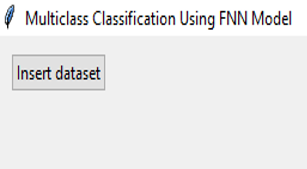
\includegraphics[width=\linewidth]{SSprogram/01Awal.png}  
  \caption{}
  \label{fig: ss 01}
\end{subfigure}
\begin{subfigure}[h]{0.49\textwidth}
  \centering
  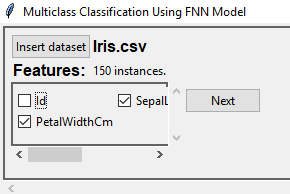
\includegraphics[width=.7\linewidth]{SSprogram/02-Select-features.png}
  \caption{}
  \label{fig: ss 02}
\end{subfigure}
\caption{Tampilan awal program}
\label{fig: tampilan awal}
\end{figure}

\noindent Program ini menyediakan beberapa pilihan untuk tahap pra pemrosesan data. Pada \ref{fig: ss 03}, kotak berwarna biru digunakan untuk menentukan fitur-fitur yang berupa kategori. Di samping itu, pengguna memiliki pilihan terkait data uji yang digunakan. Pilihan ini disediakan pada kotak merah (\ref{fig: ss 03}). Jika data uji yang digunakan terpisah dari data yang telah dimasukkan, maka nantinya pengguna harus memasukkan data uji. Jika data uji ingin dipisahkan menggunakan program ini yang dibantu oleh \emph{package sklearn} python, maka pengguna harus memasukkan ukuran data uji dan \emph{random state} seperti pada kotak biru di dalam \ref{fig: ss 04}. Untuk setiap data, dua nilai yang ada di kotak biru ini dibuat tetap sebagaimana yang tercantum di dalam gambar.

\begin{figure}[h!]
\begin{subfigure}[h]{\textwidth}
  \centering
  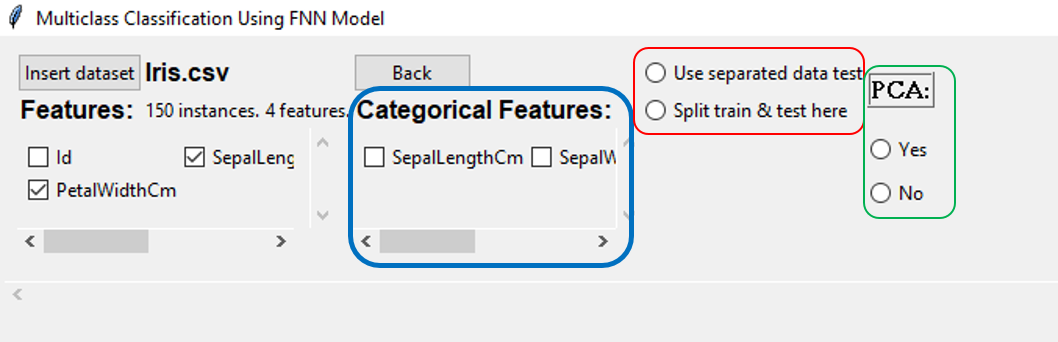
\includegraphics[width=.98\linewidth]{SSprogram/03.png}  
  \caption{}
  \label{fig: ss 03}
\end{subfigure}
\\
\begin{subfigure}[h]{\textwidth}
  \centering
  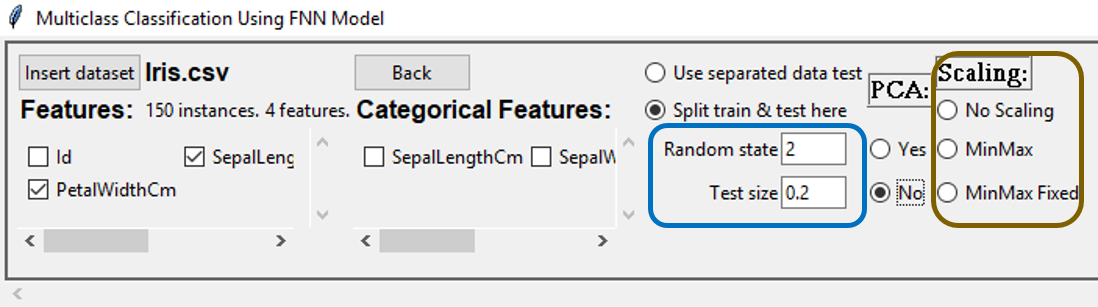
\includegraphics[width=.98\linewidth]{SSprogram/04.png}
  \caption{}
  \label{fig: ss 04}
\end{subfigure}%
\\
\begin{subfigure}[h]{\textwidth}
  \centering
  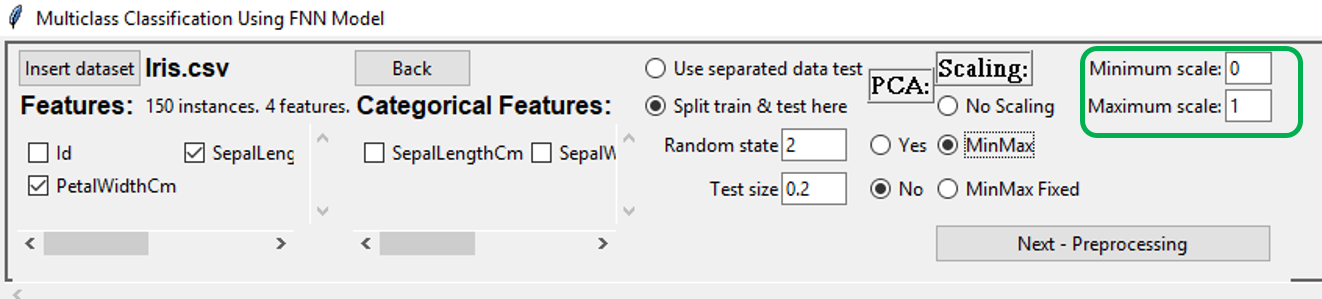
\includegraphics[width=.98\linewidth]{SSprogram/05.png}  
  \caption{}
  \label{fig: ss 05}
\end{subfigure}
\caption{Pilihan yang disediakan oleh program pada tahap pra pemrosesan data}
\label{fig: pra pemrosesan}
\end{figure}

\noindent Pilihan untuk menggunakan PCA atau tidak menggunakannya juga disediakan oleh program ini. Jika ingin menggunakan PCA, maka program secara otomatis akan menggunakan normalisasi standar untuk penskalaan dan pengguna akan diminta untuk memasukkan banyaknya komponen utama yang diinginkan. Jika tidak, maka pengguna akan memilih jenis penskalaan nilai pada data latih sesuai dengan yang tertera di dalam kotak berwarna emas pada \ref{fig: ss 04}. Pilihan `\emph{MinMax Fixed}' digunakan ketika fitur-fitur pada data memiliki skala nilai yang sama, diketahui nilai minimum dan maksimumnya, serta nilai-nilai dari fitur berpeluang tidak dapat diterima oleh model JSF. Pilihan `\emph{MinMax Fixed}' dan `\emph{MinMax}' sama-sama akan meminta nilai skala minimal dan maksimal yang diinginkan (\ref{fig: ss 05}). Selanjutnya, dengan menekan tombol `\colorbox{gray!30}{Next - Preprocessing}', maka program akan melakukan pra pemrosesan data sesuai dengan pilihan pengguna yang telah dibahas sebelumnya.

\begin{figure}[h!]
\begin{subfigure}[h]{\textwidth}
  \centering
  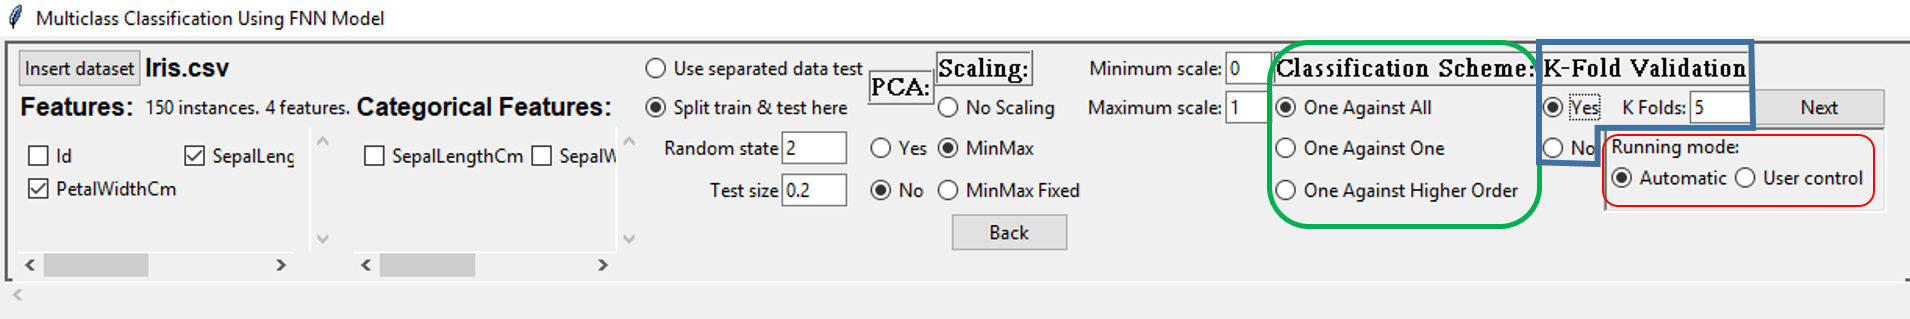
\includegraphics[width=.98\linewidth]{SSprogram/06.png}  
  \caption{}
  \label{fig: ss 06}
\end{subfigure}
\\
\begin{subfigure}[h]{\textwidth}
  \centering
  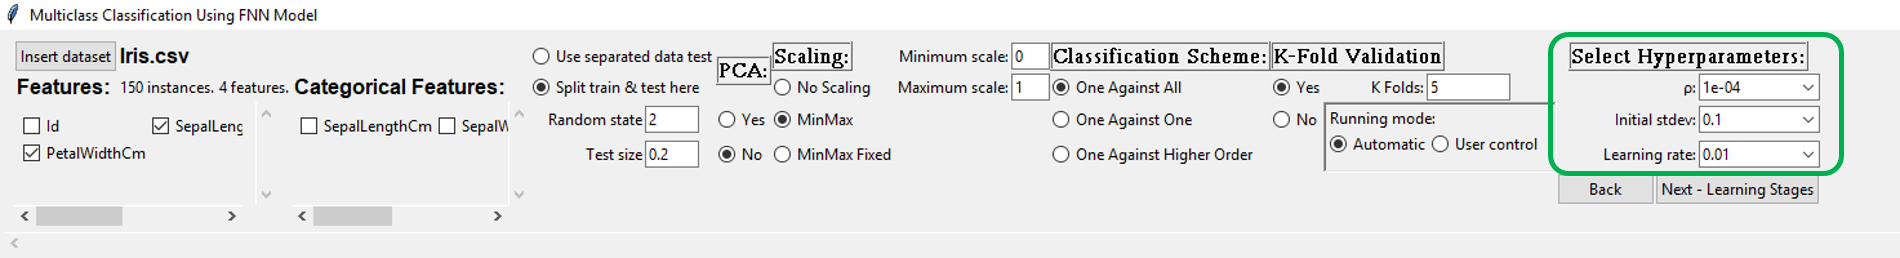
\includegraphics[width=.98\linewidth]{SSprogram/07.png}
  \caption{}
  \label{fig: ss 07}
\end{subfigure}%
\\
\begin{subfigure}[h]{\textwidth}
  \centering
  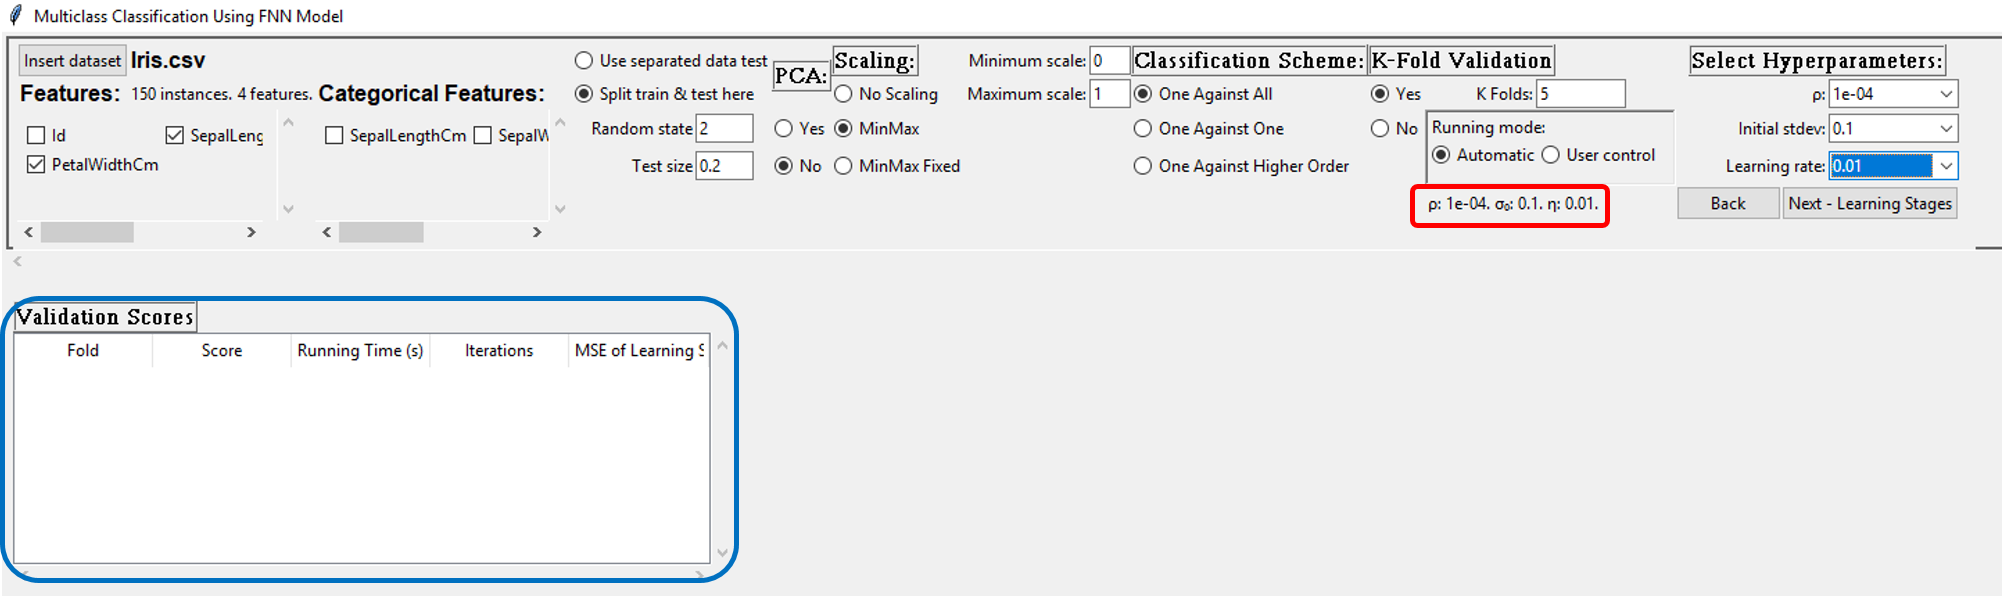
\includegraphics[width=.98\linewidth]{SSprogram/08.png}  
  \caption{}
  \label{fig: ss 08}
\end{subfigure}
\caption{Pemilihan skema klasifikasi multikelas, validasi silang, dan hiperparameter}
\label{fig: skema klas, cv, dan hyperpar}
\end{figure}

\noindent \ref{fig: skema klas, cv, dan hyperpar} menunujukkan bahwa program ini dapat menyediakan berbagai pilihan untuk menentukan skema ML. Di dalam kotak hijau pada \ref{fig: ss 06} pengguna dapat memilih skema klasifikasi multikelas yang akan digunakan. Pilihan \emph{running mode} di dalam kotak merah pada \ref{fig: ss 06} menyediakan pilihan mode untuk menjalankan skema pembangunan model JSF. Jika pengguna ingin menentukan nilai dari batas galat dan iterasi maksimal secara manual, serta ingin melanjutkan \emph{running} ke sub data latih berikutnya dengan cara manual, maka gunakan pilihan `\emph{user control}'. Jika pengguna menginginkan program secara otomatis dapat membangun dan menguji model JSF dari awal sampai dengan selesai, maka gunakan pilihan `\emph{automatic}'. Ketika memilih pilihan ini, maka nilai dari batas galat dan iterasi maksimal, berturut-turut, ditetapkan sebesar $10^{-4}$ dan 1.000. Sebagian besar data dan skema klasifikasi multikelas menggunakan pilihan `\emph{automatic}' untuk membangun model JSF berdasarkan data tersebut.

\noindent Pilihan antara akan menggunakan validasi silang atau tidak menggunakannya terdapat di dalam kotak biru pada \ref{fig: ss 06}. Lebih jauh lagi, jika pengguna memilih untuk menggunakan validasi silang, program ini akan menyediakan fasilitas berupa banyaknya \emph{fold} (sub data latih) yang diinginkan. Pada skema pembangunan model JSF dan pengujian setiap data di dalam tugas akhir ini, pilihan ``tidak menggunakan validasi silang'' digunakan ketika hiperparameter `terbaik' telah diperoleh untuk suatu skema klasifikasi multikelas.

\noindent Bagian yang cukup penting dalam skema pembangunan model ML, termasuk model JSF, adalah penentuan nilai dari hiperparameter. Penentuan nilai-nilai hiperparameter disediakan di dalam kotak hijau pada \ref{fig: ss 07}. Pada tugas akhir ini, hiperparameter yang akan berubah-ubah adalah $\rho$, $s_0$, dan $\eta$. Nilai $\tau$ dijadikan tetap.

\noindent Berikut ini adalah penjelasan mengenai alasan dari nilai $\tau$ yang dijadikan tetap. Berdasarkan penjelasan pada Subbab \ref{skema klasifikasi}, setiap skema klasifikasi multikelas mengakibatkan model JSF hanya bernilai 0 atau 1 pada semua neuron di dalam lapisan keluaran. Dalam skema OAA, nilai neuron-neuron pada lapisan keluaran dari observasi ke-$l$ dinyatakan dengan $\mathbf{d}^{(l)} = (d^{(l)}_1, d^{(l)}_2, \ldots, d^{(l)}_p)$ dengan $p$ menyatakan banyaknya label kelas yang berbeda pada data. Pada skema OAA, jika observasi ke-$l$ memiliki label kelas $\mathcal{C}_k$, maka entri ke-$k$ dari vektor $\mathbf{d}^{(l)}$ bernilai 1 dan entri yang tersisa bernilai 0. Akibatnya, nilai dari $u$ pada (\ref{kriteria kemiripan keluaran}) selalu sama dengan $\sqrt{2}$. Dalam skema OAO dan OAHO, nilai neuron pada lapisan keluaran dari setiap jaringannya hanya di antara 0 atau 1. Akibatnya, nilai dari $u$ pada (\ref{kriteria kemiripan keluaran}) selalu sama dengan $1$. Dengan demikian, untuk setiap $\tau<1$ pada Pertidaksamaan (\ref{kriteria kemiripan keluaran}) akan menghasilkan keputusan yang sama terkait kemiripan data keluaran dengan klaster yang telah terbentuk dalam fase identifikasi struktur. Jadi, nilai hiperparameter $\tau$ dapat dijadikan tetap. Pada model JSF yang dibangun melalui tugas akhir ini, ditetapkan $\tau = \num{0,3}$.

\noindent Nilai hiperparameter $\rho$ dipilih dari himpunan $\{ 10^{-4}\text{, } \allowbreak 10^{-8} \text{, } \allowbreak 10^{-12} \text{, } \allowbreak 10^{-20} \text{, } \allowbreak 10^{-25} \text{, } \allowbreak 10^{-50} \text{, } \allowbreak 10^{-75} \text{, } \allowbreak 10^{-125} \text{, } \allowbreak 10^{-200} \text{, } \allowbreak 10^{-275} \text{, } \allowbreak 10^{-350} \}$. Nilai $\rho$ yang sangat kecil digunakan ketika data berdimensi cukup besar atau nilai simpangan baku dari fitur-fiturnya cukup besar. Nilai hiperparameter $s_0$ dipilih dari himpunan $\{\num{0,1} \text{, } \allowbreak \num{0,2} \text{, } \allowbreak \num{0,25} \text{, } \allowbreak \num{0,3} \text{, } \allowbreak \num{0,4} \text{, } \num{0,5} \text{, } \allowbreak \num{0,6}\}$ yang setiap anggotanya dikalikan dengan selisih antara nilai miksimum dan minimum dari keseluruhan nilai fitur. Nilai hiperparameter $\eta$ dipilih dari himpunan $\{\num{0,01} \text{, } \allowbreak \num{0,05} \text{, } \allowbreak \num{0,1}\}$.

\noindent Setelah setiap hiperparameter dipilih, maka program akan menampilkan nilai-nilai hiperparameter yang akan digunakan, sebagaimana tertera di dalam kotak merah pada \ref{fig: ss 08}. Selain itu, akan ditampilkan juga tabel skor akurasi untuk validasi silang pada kotak biru. Tabel ini akan terisi ketika satu iterasi dari proses validasi silang telah selesai. Selanjutnya, gunakan tombol `\colorbox{gray!30}{Next - Learning Stages}' untuk memasuki tahap utama dari pembelajaran mesin ini.

\begin{figure}[h!]
\begin{subfigure}[h]{\textwidth}
  \centering
  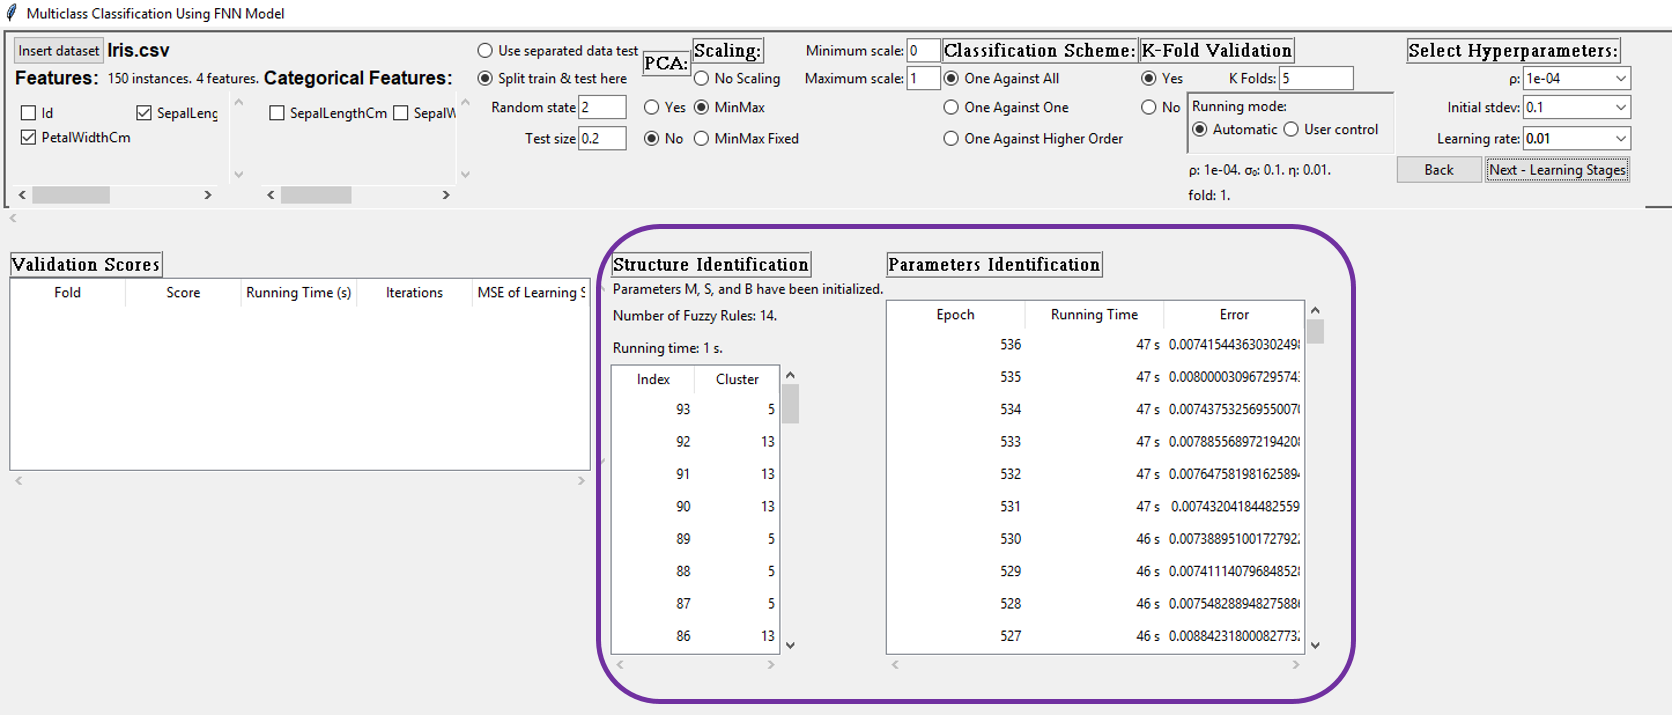
\includegraphics[width=.93\linewidth]{SSprogram/09.png}  
  \caption{Skema OAA}
  \label{fig: ss 09}
\end{subfigure}
\\
\begin{subfigure}[h]{0.5\textwidth}
  \centering
  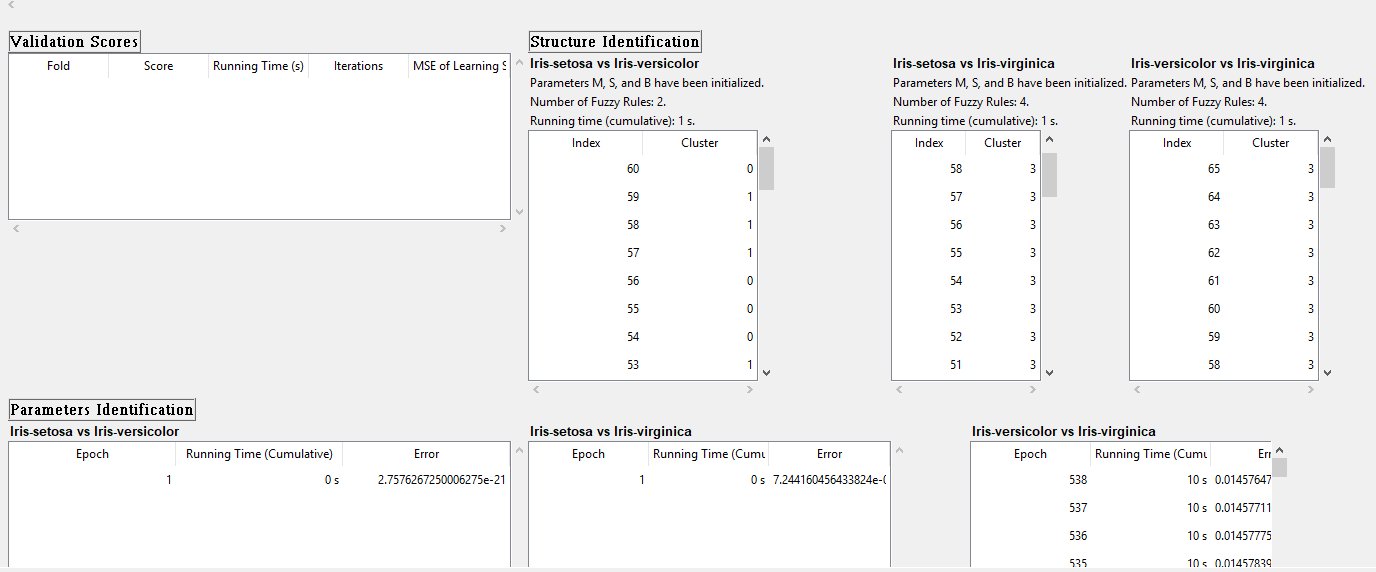
\includegraphics[width=.98\linewidth]{SSprogram/09b.png}
  \caption{Skema OAO}
  \label{fig: ss 09b}
\end{subfigure}%
\begin{subfigure}[h]{0.5\textwidth}
  \centering
  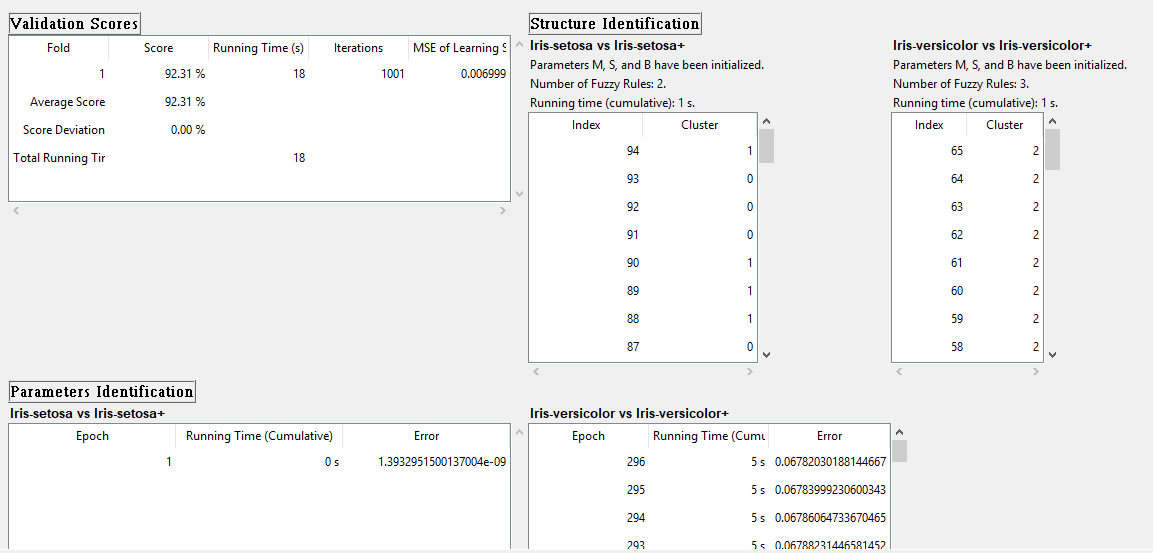
\includegraphics[width=.93\linewidth]{SSprogram/09c.png}  
  \caption{Skema OAHO}
  \label{fig: ss 09c}
\end{subfigure}
\caption{Proses pembangunan dan pengujian model jaringan saraf fuzzy}
\label{fig: proses pembelajaran dan pengujian}
\end{figure}

\noindent Proses pembangunan model ditampilkan seperti pada \ref{fig: proses pembelajaran dan pengujian}. Pada gambar tersebut ditampilkan contoh proses pembangunan model JSF dengan skema yang berbeda. Setiap skema klasifikasi multikelas memiliki tampilan yang berbeda-beda karena banyaknya jaringan yang terbentuk juga berbeda. Dalam kotak berwarna ungu pada \ref{fig: ss 09}, skema OAA hanya melakukan satu kali fase identifikasi struktur dan identifikasi parameter. Ini dikarenakan skema OAA hanya membentuk satu jaringan dari model JSF. Sebagaimana telah dijelaskan pada Subbab \ref{skema klasifikasi} bahwa skema OAO dan OAHO menghasilkan model JSF dengan jaringan berganda. Akibatnya, skema OAO dan OAHO (\ref{fig: ss 09b} dan \ref{fig: ss 09c}) melakukan lebih dari satu kali identifikasi struktur dan identifikasi parameter.

\begin{figure}[h!]
\begin{subfigure}[h]{\textwidth}
  \centering
  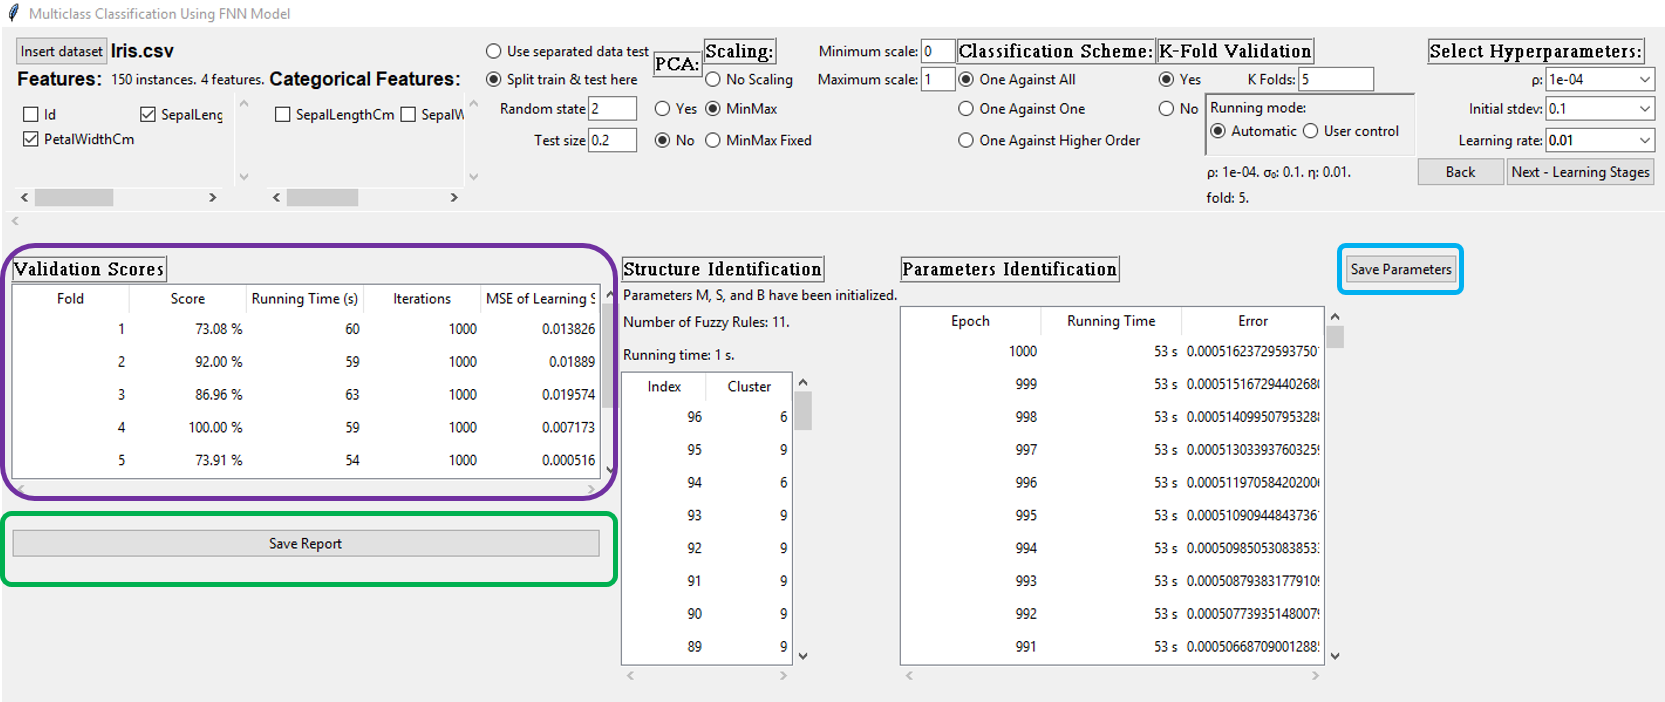
\includegraphics[width=.98\linewidth]{SSprogram/10.png}  
  \caption{}
  \label{fig: ss 10}
\end{subfigure}
\\
\begin{subfigure}[h]{\textwidth}
  \centering
  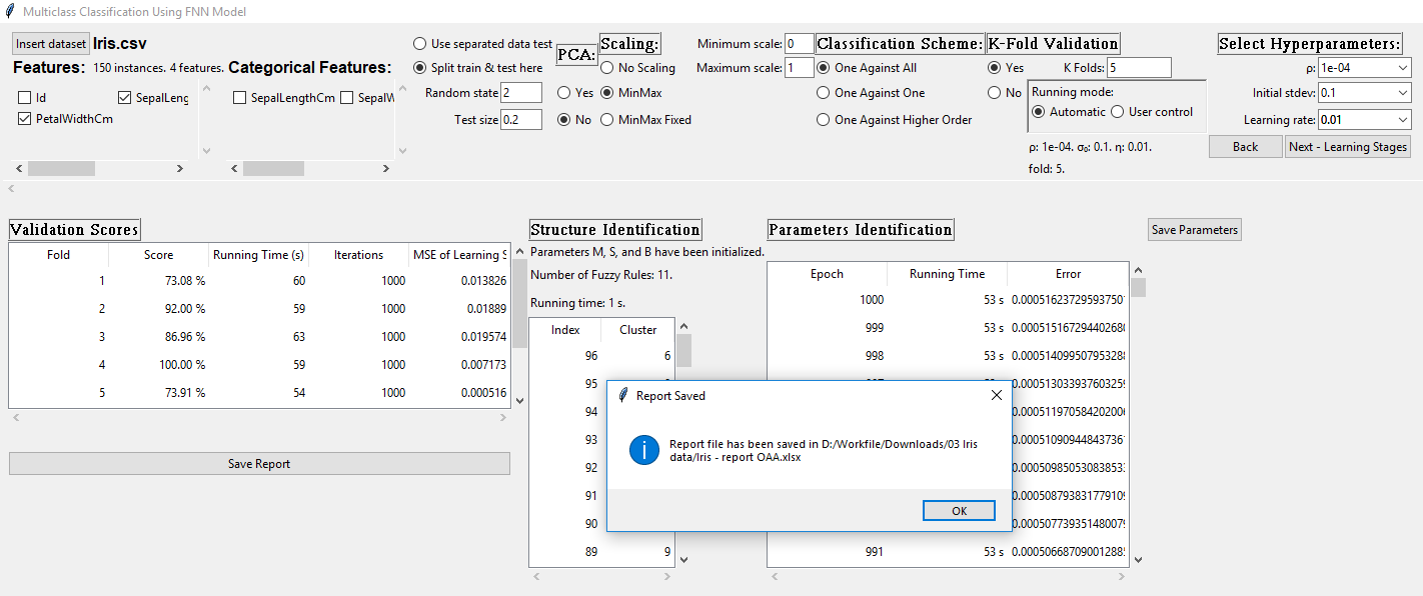
\includegraphics[width=.98\linewidth]{SSprogram/11.png}
  \caption{}
  \label{fig: ss 11}
\end{subfigure}%
\caption{Proses penyimpanan hasil uji}
\label{fig: proses penyimpanan hasil uji}
\end{figure}

\noindent Jika satu kali validasi silang telah diproses, maka akan ditampilkan skor akurasi dari data validasi seperti yang tertera di dalam kotak ungu pada \ref{fig: ss 10}. Setelah semua validasi silang selesai, maka pengguna dapat menekan tombol `\colorbox{gray!30}{Save Report}' (yang ada di dalam kotak berwarna hijau) untuk menyimpan skor akurasi dari setiap data validasi berdasarkan hiperparameter tertentu ke dalam \emph{Ms. Excel}. \ref{fig: ss 11} menunjukkan bahwa proses penyimpanan file yang diinginkan berjalan dengan lancar. Selain itu, juga diperlihatkan lokasi dan nama file yang telah disimpan. Tombol `\colorbox{gray!30}{Save Parameters}' di dalam lingkaran biru pada \ref{fig: ss 10} berfungsi untuk menyimpan nilai-nilai dari parameter yang diperoleh, yaitu matriks $\mathbf{M}$, $\mathbf{S}$, dan kumpulan matriks $\mathbf{B}_i$ ke dalam \emph{Ms. Excel}.

\noindent Proses validasi silang tersebut dilakukan berulang-ulang menggunakan nilai hiperparameter yang berbeda. Setelah model JSF memiliki skor akurasi yang optimal, maka hiperparameter yang terlibat dalam skema pembangunan model JSF tersebut digunakan untuk mendapatkan model JSF berdasarkan data latih secara keseluruhan, bukan dari beberapa sub data latih. Setelah itu, model yang diperoleh akan diuji terhadap data uji untuk mendapatkan skor akurasi model pada data uji.

\section{Deskripsi dan Analisis Data} \label{tentang data}
\noindent Data yang digunakan di antaranya adalah data koordinat I, data koordinat II, data tanaman iris, dan data evaluasi mobil. Dua data pertama dibangkitkan menggunakan bahasa pemrograman python. Dua data terakhir diambil dari situs web UCI \emph{Machine Learning Repository}. Tiga data pertama merupakan data yang seimbang. Hal ini dikarenakan setiap tiga data tersebut memiliki kardinalitas yang sama untuk setiap label kelasnya. Selain itu, nilai dari fitur-fitur pada tiga data pertama berupa bilangan real. Nilai dari fitur-fitur pada data terakhir berupa kategori. Data-data tersebut belum dipisahkan menjadi data latih dan data uji. Oleh karena itu, untuk setiap data akan dipisahkan menjadi data latih dan data uji pada tahap pra pemrosesan data.

\noindent Sebelum setiap data digunakan untuk membangun dan menguji model dan skema JSF, akan dilakukan analisis terhadap masing-masing data terlebih dahulu.Pada analisis data ini, dari masing-masing data akan dicari rata-rata, simpangan baku, median, nilai minimal, dan nilai maksimal untuk setiap fitur yang berupa bilangan real. Untuk fitur yang berupa kategori, akan dicari kardinalitas setiap kategorinya.

\subsection{Data Koordinat I} \label{tentang dk1}
\noindent Data koordinat I terdiri dari 1.000 observasi. Setiap observasi mempunyai tiga fitur yang masing-masing menjelaskan koordinat observasi tersebut pada sumbu $x$, $y$, dan $z$. Nilai-nilai untuk setiap fitur pada setiap observasi hanya berupa bilangan bulat. Label pada data koordinat I berupa nomor oktan. Banyaknya nomor oktan yang berbeda ada 8. Dengan demikian, data ini terdiri dari 8 label kelas.

\noindent Data ini terdiri dari tiga fitur. Akibatnya, setiap observasi yang ada di dalam data ini merupakan rangkap tiga terurut dari bilangan bulat. Pada data koordinat I, rangkap tiga terurut ini dibangkitkan dengan cara menentukan permutasi tiga angka yang diambil dari himpunan $U_1 = \{-5\leq u \leq -1 \text{ atau } 1 \leq u \leq 5 : u \in \mathbb{Z} \}$. Banyaknya permutasi yang mungkin adalah 1.000. Dengan demikian, semua permutasi termuat di dalam data koordinat I. Selanjutnya, setiap observasi diberi label berupa nomor oktan berdasarkan tanda pada masing-masing fiturnya. Karena semua permutasi termuat di dalam data, maka kardinalitas untuk masing-masing label kelas pada data ini adalah sama, yaitu 125. Data koordinat I dilampirkan pada Lampiran \ref{lam: data koord I}. Berikut ini hanya ditampilkan statistika deskriptifnya saja.

\begin{table}[htbp!]
  \centering
  \caption{Statistika deskriptif untuk setiap fitur dari data koordinat I}
    \begin{tabular}{lrrr}
    \toprule
    \multicolumn{1}{c}{\multirow{2}[4]{*}{\textbf{Statistika deskriptif}}} & \multicolumn{3}{c}{\textbf{Fitur}} \\
\cmidrule{2-4}          & \multicolumn{1}{c}{\boldmath{}$x$\unboldmath{}} & \multicolumn{1}{c}{\boldmath{}$y$\unboldmath{}} & \multicolumn{1}{c}{\boldmath{}$z$\unboldmath{}} \\
\cmidrule{2-4}    \textbf{Median} & $\num{0}$ & $\num{0}$ & $\num{0}$ \\
    \textbf{Rata-rata} & $\num{0}$ & $\num{0}$ & $\num{0}$ \\
    \textbf{Simpangan baku} & $\num{3,318}$ & $\num{3,318}$ & $\num{3,318}$ \\
    \textbf{Minimum} & $\num{-5}$ & $\num{-5}$ & $\num{-5}$ \\
    \textbf{Maksimum} & $\num{5}$ & $\num{5}$ & $\num{5}$ \\
    \bottomrule
    \end{tabular}%
  \label{tab: stat desc dk1}%
\end{table}%

\subsection{Data Koordinat II} \label{tentang dk2}
\noindent Berikut ini adalah statistika deskriptif untuk masing-masing fitur dari data koordinat II.

\begin{table}[htbp!]
  \centering
  \caption{Statistika deskriptif untuk setiap fitur dari data koordinat II}
    \begin{tabular}{lrrr}
    \toprule
    \multicolumn{1}{c}{\multirow{2}[4]{*}{\textbf{Statistika deskriptif}}} & \multicolumn{3}{c}{\textbf{Fitur}} \\
\cmidrule{2-4}          & \multicolumn{1}{c}{\boldmath{}$x$\unboldmath{}} & \multicolumn{1}{c}{\boldmath{}$y$\unboldmath{}} & \multicolumn{1}{c}{\boldmath{}$z$\unboldmath{}} \\
\cmidrule{2-4}    \textbf{Median} & $\num{0}$ & $\num{0}$ & $\num{0}$ \\
    \textbf{Rata-rata} & $\num{-0,091}$ & $\num{0,255}$ & $\num{0,022}$ \\
    \textbf{Simpangan baku} & $\num{56,61}$ & $\num{58,32}$ & $\num{59,04}$ \\
    \textbf{Minimum} & $\num{-100}$ & $\num{-100}$ & $\num{-100}$ \\
    \textbf{Maksimum} & $\num{100}$ & $\num{100}$ & $\num{100}$ \\
    \bottomrule
    \end{tabular}%
  \label{tab: stat desc dk2}%
\end{table}%

\noindent Data koordinat II mirip dengan data koordinat I. Perbedaannya terletak pada bilangan bulat rangkap tiga terurut yang dibangkitkan. Pada data koordinat II, rangkap tiga terurut adalah sebanyak 1.000 permutasi tiga angka dari himpunan $U_2 = \{-100\leq u \leq -1 \text{ atau } 1 \leq u \leq 100 : u \in \mathbb{Z} \}$. Banyaknya permutasi adalah $200^3 = 8\times 10^6$. Dengan demikian, hanya $\num{0,0125}\%$ dari semua kemuangkinan permutasi  yang termuat di dalam data koordinat II. Kardinalitas untuk masing-masing label kelas pada data ini dibuat sama, yaitu 125. Data ini dilampirkan pada Lampiran \ref{lam: data koord II}.

\subsection{Data Tanaman Iris} \label{tentang d iris}
\noindent Data ini memuat 3 kelas yang masing-masing terdiri dari 50 observasi. Setiap kelas mengacu pada jenis tanaman iris, yaitu: iris \emph{setosa}, iris \emph{versicolor}, dan iris \emph{virginica}. Setiap observasi memiliki 4 fitur, yaitu: panjang sepal (cm), lebar sepal (cm), panjang kelopak (cm), dan lebar kelopak (cm). Data tanaman iris merupakan data yang paling dikenal dan paling sering ditemukan dalam literatur pengenalan pola yang termasuk ke dalam masalah klasifikasi multikelas \cite{Dua:2019}. Data ini dilampirkan pada Lampiran \ref{lam: data iris}. Berikut ini hanya ditampilkan statistika deskriptifnya saja.

\begin{table}[htbp!]
  \centering
  \caption{Statistika deskriptif untuk setiap fitur dari data tanaman iris}
    \begin{tabular}{lrrrr}
    \toprule
    \multicolumn{1}{c}{\multirow{2}[3]{*}{\textbf{Statistika deskriptif}}} & \multicolumn{4}{c}{\textbf{Fitur}} \\
\cmidrule{2-5}    \multicolumn{1}{c}{} & \multicolumn{1}{>{\centering\arraybackslash} m{3.515em}}{\textbf{Panjang sepal}} & \multicolumn{1}{>{\centering\arraybackslash} m{3.115em}}{\textbf{Lebar sepal}} & \multicolumn{1}{>{\centering\arraybackslash} m{3.515em}}{\textbf{Panjang kelopak}} & \multicolumn{1}{>{\centering\arraybackslash} m{3.515em}}{\textbf{Lebar kelopak}} \\
    \cmidrule{2-5}
    \textbf{Median} & $\num{5,8}$ & $\num{3}$ & $\num{4,35}$ & $\num{1,3}$ \\
    \textbf{Rata-rata} & $\num{5,843}$ & $\num{3,054}$ & $\num{3,759}$ & $\num{1,199}$ \\
    \textbf{Simpangan baku} & $\num{0,8281}$ & $\num{0,4336}$ & $\num{1,764}$ & $\num{0,7632}$ \\
    \textbf{Minimum} & $\num{4,3}$ & $\num{2}$ & $\num{1}$ & $\num{0,1}$ \\
    \textbf{Maksimum} & $\num{7,9}$ & $\num{4,4}$ & $\num{6,9}$ & $\num{2,5}$ \\
    \bottomrule
    \end{tabular}%
  \label{tab: stat desc iris}%
\end{table}%

\noindent 

\subsection{Data Evaluasi Mobil} \label{tentang car}
\noindent Data evaluasi mobil menceritakan spesifikasi dan klasifikasi dari 1.728 mobil. Setiap mobil pada data ini diklasifikasikan ke dalam 4 label kelas berdasarkan kualitasnya. Empat label kelas ini adalah kualitas mobil yang \emph{unaccepted}, \emph{accepted}, \emph{good}, dan \emph{very good}. Setiap label kelas memiliki banyaknya observasi yang berbeda-beda. Banyaknya mobil dengan kualitas yang \emph{unaccepted},  \emph{accepted}, \emph{good}, dan \emph{very good} berturut-turut adalah 1210, 384, 69, dan 65. Setiap mobil yang ada di dalam data ini dideskripsikan oleh 6 kategori spesifikasi, yaitu:
\begin{itemize}
    \item \emph{Buying}, yaitu kategori harga beli mobil yang meliputi \emph{very high}, \emph{high}, \emph{medium}, dan \emph{low},
    \item \emph{Maintenance}, yaitu biaya pemeliharaan mobil yang kategorinya sama dengan kategori pada spesifikasi \emph{buying},
    \item \emph{Doors}, yaitu kategori banyaknya pintu mobil, terdiri dari 4 kategori yang berbeda: dua pintu, tiga pintu, empat pintu, dan kategori lima pintu atau lebih,
    \item \emph{Persons}, yaitu kategori banyaknya maksimal orang yang berada di dalam mobil, meliputi: kategori dua orang, kategori empat orang, dan kategori lebih dari empat orangm,
    \item \emph{Lug boot}, yaitu kategori ukuran bagasi mobil yang meliputi ukuran kecil, sedang, dan besar,
    \item \emph{Safety}, yaitu tingkat keamanan bagi pengendara dan penumpang, meliputi tingkat keamanan rendah, sedang, dan tinggi.
\end{itemize}

\begin{table}[htbp!]
  \centering
  \caption{Kardinalitas setiap kategori pada setiap fitur dari data evaluasi mobil}
    \begin{tabular}{crcrcr}
    \toprule
    \multicolumn{2}{c}{\textit{\textbf{Buying}}} & \multicolumn{2}{c}{\textit{\textbf{Maintenance}}} & \multicolumn{2}{c}{\textit{\textbf{Doors}}} \\
    \cmidrule(r){1-2}\cmidrule(lr){3-4}\cmidrule(l){5-6}
    \textbf{Kategori} & \multicolumn{1}{c}{\textbf{Kardinalitas}} & \textbf{Kategori} & \multicolumn{1}{c}{\textbf{Kardinalitas}} & \textbf{Kategori} & \multicolumn{1}{c}{\textbf{Kardinalitas}} \\
    \cmidrule(r){1-2}\cmidrule(lr){3-4}\cmidrule(l){5-6}
    \textit{\textbf{med}} & 432   & \textit{\textbf{med}} & 432   & \textit{\textbf{two}} & 432 \\
    \textit{\textbf{high}} & 432   & \textit{\textbf{high}} & 432   & \textit{\textbf{four}} & 432 \\
    \textit{\textbf{low}} & 432   & \textit{\textbf{low}} & 432   & \textit{\textbf{three}} & 432 \\
    \textit{\textbf{vhigh}} & 432   & \textit{\textbf{vhigh}} & 432   & \textit{\textbf{5more}} & 432 \\
    \midrule
          &       &       &       &       &  \\
    \midrule
    \multicolumn{2}{c}{\textit{\textbf{Persons}}} & \multicolumn{2}{c}{\textit{\textbf{Lug boot}}} & \multicolumn{2}{c}{\textit{\textbf{Safety}}} \\
    \cmidrule(r){1-2}\cmidrule(lr){3-4}\cmidrule(l){5-6}
    \textbf{Kategori} & \multicolumn{1}{c}{\textbf{Kardinalitas}} & \textbf{Kategori} & \multicolumn{1}{c}{\textbf{Kardinalitas}} & \textbf{Kategori} & \multicolumn{1}{c|}{\textbf{Kardinalitas}} \\
    \cmidrule(r){1-2}\cmidrule(lr){3-4}\cmidrule(l){5-6}
    \textit{\textbf{two}} & 576   & \textit{\textbf{big}} & 576   & \textit{\textbf{med}} & 576 \\
    \textit{\textbf{four}} & 576   & \textit{\textbf{med}} & 576   & \textit{\textbf{high}} & 576 \\
    \textit{\textbf{more}} & 576   & \textit{\textbf{small}} & 576   & \textit{\textbf{low}} & 576 \\
    \bottomrule
    \end{tabular}%
  \label{tab: kard kat ev mobil}%
\end{table}%

\noindent Berdasarkan \ref{tab: kard kat ev mobil}, data evaluasi mobil memiliki kardinalitas yang seimbang antara setiap kategori pada masing-masing fiturnya. Karena semua fitur pada data ini berupa kategori, maka harus dilakukan pengkodean terlebih dahulu untuk setiap fiturnya. Pada tugas akhir ini, hanya akan dilakukan pengkodean dengan metode \emph{one hot encoding} yang telah dijelaskan pada Subbab \ref{preproccessing}. Setelah dilakukan \emph{one hot encoding}, banyaknya fitur pada data evaluasi mobil menjadi 21 dengan setiap entrinya berupa bilangan biner 0 atau 1. Data lengkap untuk data evaluasi mobil ini dilampirkan pada Lampiran \ref{lam: data mobil}.

\section{Hasil Uji} \label{hasil uji}
\noindent Pada tugas akhir ini, setiap data akan digunakan untuk membangun model JSF dengan skema tertentu dari klasifikasi multikelas. Tiga skema klasifikasi multikelas yang telah dijelaskan pada Subbab \ref{skema klasifikasi} akan digunakan untuk masing-masing data. Dengan demikian, terdapat 12 model JSF karena setiap data menghasilkan 3 model JSF dengan skema klasifikasi multikelas yang berbeda-beda.

\noindent Untuk setiap data dan skema klasifikasi, dilakukan validasi silang $K$-\emph{fold} untuk mendapatkan hiperparameter terbaik. Pada tugas akhir ini, hanya akan digunakan $K=5$, sehingga data latih dipartisi menjadi 5 sub data latih. Selanjutnya, dari 5 sub data latih ini akan diperoleh 5 \emph{learning set} dan 5 data validasi yang saling bersesuaian. Metode pembuatan 5 \emph{learning set} dan 5 data validasi ini telah dijelaskan pada Subbab \ref{pemilihan model}.

\noindent Pada validasi silang $5$-\emph{fold}, setiap \emph{learning set} akan digunakan untuk membangun model JSF dengan skema klasifikasi tertentu. Setiap model JSF yang diperoleh ini akan diuji pada data validasi. Hasil uji ini akan menghasilkan skor akurasi dari prediksi label kelas pada setiap observasi di dalam data validasi.  Dengan demikian, akan ada 5 model JSF dan 5 skor akurasi yang diperoleh. Untuk meringkas performa dari 5 model JSF ini, digunakan nilai rata-rata dan simpangan baku dari 5 skor akurasi, sebagaimana telah dijelaskan pada Subbab \ref{pemilihan model}.

\noindent Model JSF yang paling optimal akan dihasilkan ketika menggunakan hiperparameter terbaik untuk membangun model JSF tersebut. Karena terdapat lebih dari satu kombinasi hiperparameter yang mungkin, maka validasi silang $5$-\emph{fold} harus dilakukan secara berulang dengan kombinasi hiperparameter yang berbeda-beda. Setelah melakukan validasi silang $5$-\emph{fold} secara berulang, maka dapat dipilih hiperparameter yang dapat membangun 5 model JSF dengan rata-rata akurasi terbesar, simpangan baku akurasi yang cukup kecil, dan \emph{running time} yang lebih singkat. Meskipun validasi silang $5$-\emph{fold} dilakukan berulang, hasil partisi data latih tidak akan berbeda karena partisinya hanya dilakukan di awal.

\subsection{Data Koordinat I}
\noindent Berdasarkan \ref{tab: stat desc dk1}, nilai minimal dan maksimal dari fitur pada data koordinat I masih dapat diterima oleh model JSF. Selain itu, setiap fiturnya memiliki satuan yang sama. Oleh karena itu, tidak akan ada proses normalisasi terhadap fitur-fitur pada data ini. Pra pemrosesan data yang dilakukan terhadap data ini hanya pemisahan data latih dan data uji. Setelah dilakukan pemisahan data latih dan data uji yang dilanjutkan dengan partisi data latih ke dalam 5 bagian, diperoleh banyaknya observasi yang dikelompokkan berdasarkan label kelasnya (\ref{tab: label kelas dk1}).

\begin{table}[h!]
  \centering
  \caption{Kardinalitas label kelas pada data koordinat I}
    \begin{tabular}{lrrrr}
    \toprule
          & \multicolumn{1}{c}{\textbf{Oktan I}} & \multicolumn{1}{c}{\textbf{Oktan II}} & \multicolumn{1}{c}{\textbf{Oktan III}} & \multicolumn{1}{c}{\textbf{Oktan IV}} \\
    \midrule
    \textbf{Data asli} & 125   & 125   & 125   & 125 \\
    \textbf{Data latih} & 98    & 89    & 101   & 102 \\
    \textbf{Sub data latih 1} & 20    & 18    & 21    & 21 \\
    \textbf{Sub data latih 2} & 20    & 18    & 20    & 21 \\
    \textbf{Sub data latih 3} & 20    & 18    & 20    & 20 \\
    \textbf{Sub data latih 4} & 19    & 18    & 20    & 20 \\
    \textbf{Sub data latih 5} & 19    & 17    & 20    & 20 \\
    \textbf{Data uji} & 27    & 36    & 24    & 23 \\
    \midrule
          &       &       &       &  \\
    \midrule
          & \multicolumn{1}{c}{\textbf{Oktan V}} & \multicolumn{1}{c}{\textbf{Oktan VI}} & \multicolumn{1}{c}{\textbf{Oktan VII}} & \multicolumn{1}{c}{\textbf{Oktan VIII}} \\
    \midrule
    \textbf{Data asli} & 125   & 125   & 125   & 125 \\
    \textbf{Data latih} & 106   & 102   & 101   & 101 \\
    \textbf{Sub data latih 1} & 22    & 21    & 21    & 21 \\
    \textbf{Sub data latih 2} & 21    & 21    & 20    & 20 \\
    \textbf{Sub data latih 3} & 21    & 20    & 20    & 20 \\
    \textbf{Sub data latih 4} & 21    & 20    & 20    & 20 \\
    \textbf{Sub data latih 5} & 21    & 20    & 20    & 20 \\
    \textbf{Data uji} & 19    & 23    & 24    & 24 \\
    \bottomrule
    \end{tabular}%
  \label{tab: label kelas dk1}%
\end{table}%

\subsubsection{Skema OAA}
\noindent \ref{tab: dk1 OAA} adalah daftar ringkasan dari performa semua model JSF dengan skema OAA berdasarkan 5 \emph{learning set} pada data koordinat I.  Masing-masing ringkasan ini diperoleh dengan cara melakukan validasi silang 5-\emph{fold} dengan hiperparameter yang berbeda-beda. Rata-rata dan simpangan baku akurasi dihitung menggunakan (\ref{rataan akurasi}) dan (\ref{sd akurasi}) berturut-turut.

\begin{table}[htbp!]
  \centering
  \caption{Hasil validasi silang 5-\emph{fold} data latih pada data koordinat I dengan skema OAA}
    \begin{tabular}{rrrrrr}
    \toprule
    \multicolumn{3}{c}{\textbf{Hiperparameter}} & \multicolumn{3}{c}{ \textbf{Performa model JSF} }\\
    \cmidrule(r){1-3}\cmidrule(l){4-6}
    \multicolumn{1}{ >{\centering\arraybackslash} m{2.215em}}{$\boldsymbol{\rho}$} & \multicolumn{1}{ >{\centering\arraybackslash} m{2.215em}}{\boldmath{}$s_0$\unboldmath{}} & \multicolumn{1}{ >{\centering\arraybackslash} m{2.215em}}{$\boldsymbol{\eta}$} & \multicolumn{1}{ >{\centering\arraybackslash} m{3.785em}}{\textbf{Rata-rata akurasi}} & \multicolumn{1}{ >{\centering\arraybackslash} m{4.5em}}{\textbf{Simpangan baku akurasi}} & \multicolumn{1}{ >{\centering\arraybackslash} m{4.34em}}{\textbf{\emph{Total Running Time} (s)}} \\
    \cmidrule(r){1-3}\cmidrule(l){4-6}
    $10^{-4}$ & 1     & 0,01  & 90,05\% & 5,15\% & 4657 \\
    $10^{-4}$ & 1     & 0,05  & 90,05\% & 5,15\% & 4669 \\
    $10^{-8}$ & 1     & 0,01  & 100,00\% & 0,00\% & 2178 \\
    \bottomrule
    \end{tabular}%
  \label{tab: dk1 OAA}%
\end{table}%

\noindent Karena telah diperoleh rata-rata akurasi yang besarnya $100\%$, maka perulangan berhenti. Dengan demikian, hiperparameter $\boldsymbol{\theta} = (\rho, s_0,\eta) = (10^{-8}\text{,  } \allowbreak 1\text{,  } \allowbreak \num{0,01})$ adalah hiperparameter terbaik untuk data koordinat I yang dimodelkan menggunakan skema OAA. Selanjutnya, hiperparameter ini digunakan untuk membangun model JSF dengan skema OAA berdasarkan data latih dari data koordinat I. Kemudian, parameter yang telah diperoleh berdasrkan skema pembangunan model JSF, digunakan untuk memprediksi label kelas pada data uji. Setelah dilakukan prediksi pada data uji, maka diperoleh akurasi dari prediksi tersebut. Akurasi yang diperoleh adalah $100\%$ juga dan durasi waktu yang dibutuhkan untuk membangun model JSF adalah selama $499$ detik.

\subsubsection{Skema OAO}
\noindent  Performa semua model JSF dari data latih pada data koordinat I dengan skema OAO diringkas pada \ref{tab: dk1 OAO}.  Masing-masing ringkasan ini diperoleh dengan cara melakukan validasi silang 5-\emph{fold} dengan hiperparameter yang berbeda-beda.
\begin{table}[htbp!]
  \centering
  \caption{Hasil validasi silang 5-\emph{fold} data latih pada data koordinat I dengan skema OAO}
    \begin{tabular}{crrrrr}
    \toprule
    \multicolumn{3}{c}{\textbf{Hiperparameter}} & \multicolumn{3}{c}{ \textbf{Performa model JSF} }\\
    \cmidrule(r){1-3}\cmidrule(l){4-6}
    \multicolumn{1}{ >{\centering\arraybackslash} m{2.215em}}{$\boldsymbol{\rho}$} & \multicolumn{1}{ >{\centering\arraybackslash} m{2.215em}}{\boldmath{}$s_0$\unboldmath{}} & \multicolumn{1}{ >{\centering\arraybackslash} m{2.215em}}{$\boldsymbol{\eta}$} & \multicolumn{1}{ >{\centering\arraybackslash} m{3.785em}}{\textbf{Rata-rata akurasi}} & \multicolumn{1}{ >{\centering\arraybackslash} m{4.355em}}{\textbf{Simpangan baku akurasi}} & \multicolumn{1}{ >{\centering\arraybackslash} m{4.34em}}{\textbf{\emph{Total Running Time} (s)}} \\
    \cmidrule(r){1-3}\cmidrule(l){4-6}
    $10^{-4}$ & 1     & 0,01  & 91,92\% & 4,59\% & 2215 \\
    $10^{-8}$ & 1     & 0,01  & 100,00\% & 0,00\% & 1373 \\
    \bottomrule
    \end{tabular}%
  \label{tab: dk1 OAO}%
\end{table}%

\noindent Berdasarkan \ref{tab: dk1 OAO}, diperoleh hiperparameter $\boldsymbol{\theta} = (\rho, s_0,\eta) = (10^{-8}\text{,  } \allowbreak 1\text{,  } \allowbreak \num{0,01})$ sebagai hiperparameter terbaik untuk data koordinat I yang dimodelkan dengan skema OAO. Hiperparameter ini menyebabkan rata-rata akurasi yang dicapai oleh model sebesar $100\%$. Meskipun memiliki hiperparameter terbaik yang sama dengan skema OAA, skema OAO memiliki durasi waktu yang lebih singkat untuk membangun model JSF. Hal ini dikarenakan setiap jaringan dari $28$ jaringan yang dibangun memiliki \emph{learning set} yang sedikit. Selain itu, iterasi yang diperlukan pada fase identifikasi parameter untuk setiap jaringannya banyak yang tidak mencapai 1.000 kali iterasi.

\noindent Setelah hiperparameter $\boldsymbol{\theta}$ digunakan untuk membangun model JSF pada data latih dengan skema OAO, diperoleh akurasi dari data uji sebesar $100\%$. Waktu yang diperlukan untuk membangun model JSF dengan skema OAO adalah selama $331$ detik. %Parameter yang diperoleh untuk model JSF dengan skema OAA pada data ini dilampirkan pada Lampiran \ref{lam: dk1 OAO}.

\subsubsection{Skema OAHO}
\noindent Performa semua model JSF dengan skema OAHO berdasarkan 5 \emph{learning set} pada data koordinat I diringkas pada \ref{tab: dk1 OAHO}.  Masing-masing ringkasan ini diperoleh dengan cara melakukan validasi silang 5-\emph{fold} dengan hiperparameter yang berbeda-beda.

\begin{table}[htbp!]
  \centering
  \caption{Hasil validasi silang 5-\emph{fold} data latih pada data koordinat I dengan skema OAHO}
    \begin{tabular}{lrrrrr}
    \toprule
    \multicolumn{3}{c}{\textbf{Hiperparameter}} & \multicolumn{3}{c}{ \textbf{Performa model JSF} }\\
    \cmidrule(r){1-3}\cmidrule(l){4-6}
    \multicolumn{1}{ >{\centering\arraybackslash}  m{2.215em}}{$\boldsymbol{\rho}$} & \multicolumn{1}{ >{\centering\arraybackslash} m{2.215em}}{\boldmath{}$s_0$\unboldmath{}} & \multicolumn{1}{ >{\centering\arraybackslash} m{2.215em}}{$\boldsymbol{\eta}$} & \multicolumn{1}{ >{\centering\arraybackslash} m{3.785em}}{\textbf{Rata-rata akurasi}} & \multicolumn{1}{ >{\centering\arraybackslash} m{4.355em}}{\textbf{Simpangan baku akurasi}} & \multicolumn{1}{ >{\centering\arraybackslash} m{4.34em}}{\textbf{\emph{Total Running Time (s)}}} \\
    \cmidrule(r){1-3}\cmidrule(l){4-6}
    $10^{-8}$ & 1     & 0,01  & 95,09\% & 4,98\% & 2016 \\
    $10^{-12}$ & 1     & 0,01  & 95,09\% & 4,98\% & 2170 \\
    $10^{-12}$ & 3     & 0,01  & 90,12\% & 12,05\% & 1937 \\
    $10^{-4}$ & 1     & 0,01  & 89,78\% & 6,00\% & 3812 \\
    $10^{-4}$ & 3     & 0,01  & 91,88\% & 9,86\% & 2299 \\
    $10^{-25}$ & 3     & 0,01  & 89,23\% & 13,82\% & 1690 \\
    \bottomrule
    \end{tabular}%
  \label{tab: dk1 OAHO}%
\end{table}%

\noindent \ref{tab: dk1 OAHO} memberikan informasi bahwa jika nilai $\rho$ semakin menjauh dari $10^{-8}$ atau $10^{-12}$, maka dapat mengakibatkan rata-rata akurasi mengecil. Oleh karena itu, perulangan dari validasi silang dihentikan setelah $\rho=10^{-25}$. Dengan demikian, hiperparameter $\boldsymbol{\theta} = (\rho, s_0,\eta) = (10^{-8}\text{,  } \allowbreak 1\text{,  } \allowbreak \num{0,01})$ adalah hiperparameter terbaik untuk model JSF dari data latih pada data koordinat I dengan skema OAHO dan akurasinya sebesar $\num{95,09}\%\pm \num{4,98}\%$. Meskipun akurasi model JSF dengan hiperparameter $\boldsymbol{\theta}$ sama dengan akurasi dari model JSF dengan hiperparameter $(10^{-12}\text{,  } \allowbreak 1\text{,  } \allowbreak \num{0,01})$, tetapi hiperparameter $\boldsymbol{\theta}$ memiliki durasi waktu yang lebih singkat.

\noindent Selanjutnya, akan dibangun model JSF dari data latih pada data koordinat I dengan skema klasifikasi OAHO dan menggunakan hiperparameter $\boldsymbol{\theta} = (10^{-8}\text{,  } \allowbreak 1\text{,  } \allowbreak \num{0,01})$. Hasil dari model ini berupa parameter-parameter yang terlibat pada $p-1$ jaringan saraf fuzzy, yaitu matriks $\mathbf{M}_{k,k^+}$, $\mathbf{S}_{k,k^+}$, dan $\mathbf{B}_{k,k^+}$ untuk $k=1,2,\ldots,p$. Kemudian nilai dari parameter-parameter ini diuji terhadap data uji dan diperoleh akurasi pada data uji sebesar $98\%$. Durasi waktu yang diperlukan untuk membangun model JSF dari data latih tersebut adalah selama $490$ detik.

\subsection{Data Koordinat II}
\noindent \ref{tab: label kelas dk2} menampilkan kardinalitas masing-masing label kelas pada data koordinat II dan pada bagian-bagiannya.
\begin{table}[h!]
  \centering
  \caption{Kardinalitas label kelas pada data koordinat II}
    \begin{tabular}{lrrrr}
    \toprule
          & \multicolumn{1}{c}{\textbf{Oktan I}} & \multicolumn{1}{c}{\textbf{Oktan II}} & \multicolumn{1}{c}{\textbf{Oktan III}} & \multicolumn{1}{c}{\textbf{Oktan IV}} \\
    \midrule
    \textbf{Data asli} & 125   & 125   & 125   & 125 \\
    \textbf{Data latih} & 99    & 100   & 104   & 102 \\
    \textbf{Sub data latih 1} & 20    & 20    & 21    & 21 \\
    \textbf{Sub data latih 2} & 20    & 20    & 21    & 21 \\
    \textbf{Sub data latih 3} & 20    & 20    & 21    & 20 \\
    \textbf{Sub data latih 4} & 20    & 20    & 21    & 20 \\
    \textbf{Sub data latih 5} & 19    & 20    & 20    & 20 \\
    \textbf{Data uji} & 26    & 25    & 21    & 23 \\
    \midrule
          &       &       &       &  \\
    \midrule
          & \multicolumn{1}{c}{\textbf{Oktan V}} & \multicolumn{1}{c}{\textbf{Oktan VI}} & \multicolumn{1}{c}{\textbf{Oktan VII}} & \multicolumn{1}{c}{\textbf{Oktan VIII}} \\
    \midrule
    \textbf{Data asli} & 125   & 125   & 125   & 125 \\
    \textbf{Data latih} & 95    & 103   & 99    & 98 \\
    \textbf{Sub data latih 1} & 19    & 21    & 20    & 20 \\
    \textbf{Sub data latih 2} & 19    & 21    & 20    & 20 \\
    \textbf{Sub data latih 3} & 19    & 21    & 20    & 20 \\
    \textbf{Sub data latih 4} & 19    & 20    & 20    & 19 \\
    \textbf{Sub data latih 5} & 19    & 20    & 19    & 19 \\
    \textbf{Data uji} & 30    & 22    & 26    & 27 \\
    \bottomrule
    \end{tabular}%
    \label{tab: label kelas dk2}
\end{table}

\noindent Berdasarkan \ref{tab: stat desc dk2}, nilai minimal dan maksimal dari fitur pada data koordinat II sangat jauh dari 0. Karena simpangan baku setiap fiturnya bernilai cukup besar dan tidak seragam, maka dapat dikatakan bahwa nilai-nilai pada setiap fitur tersebar cukup luas dan penyebaran nilai antar fiturnya sangat beragam. Akibatnya,  perlu dilakukan normalisasi terhadap fitur-fitur pada data ini. Karena dimensinya hanya tiga, maka tidak perlu dilakukan PCA terhadap fitur-fitur pada data ini. Dengan demikian, normalisasi yang akan dilakukan adalah normalisasi minimal-maksimal. Supaya tidak kehilangan makna yang berhubungan dengan nomor oktan, maka akan digunakan skala minimal $-1$ dan skala maksimal $1$ pada proses normalisasi.

\noindent Sebelum dilakukan normalisasi, dilakukan terlebih dahulu pemisahan data menjadi data latih dan data uji. Hal ini dikarenakan proses normalisasi menggunakan nilai minimal dan maksimal dari setiap fitur pada data latih. Setelah normalisasi, dilakukan partisi data latih ke dalam 5 bagian. Banyaknya observasi pada data koordinat II dan pada bagian-bagiannya yang dikelompokkan berdasarkan label kelas didaftarkan pada \ref{tab: label kelas dk2}.

\subsubsection{Skema OAA}
\noindent Performa semua model JSF dengan skema OAA berdasarkan 5 \emph{learning set} pada data koordinat II diringkas pada \ref{tab: dk2 OAA}.  Masing-masing ringkasan ini diperoleh dengan cara melakukan validasi silang 5-\emph{fold} dengan hiperparameter yang berbeda-beda.

\begin{table}[htbp!]
  \centering
  \caption{Hasil validasi silang 5-\emph{fold} data latih pada data koordinat II dengan skema OAA}
    \begin{tabular}{lrrrrr}
    \toprule
    \multicolumn{3}{c}{\textbf{Hiperparameter}} & \multicolumn{3}{c}{ \textbf{Performa model JSF} }\\
    \cmidrule(r){1-3}\cmidrule(l){4-6}
    \multicolumn{1}{ >{\centering\arraybackslash} m {2.215em}}{$\boldsymbol{\rho}$} & \multicolumn{1}{>{\centering\arraybackslash} m{2.215em} }{\boldmath{}$s_0$ \unboldmath{}} & \multicolumn{1}{>{\centering\arraybackslash} m{2.215em}}{$\boldsymbol{\eta}$} & \multicolumn{1}{>{\centering\arraybackslash} m{4.215em}}{\textbf{Rata-rata akurasi}} & \multicolumn{1}{>{\centering\arraybackslash} m{5.145em}}{\textbf{Simpangan baku akurasi}} & \multicolumn{1}{>{\centering\arraybackslash} m{3.4em}}{\textbf{\emph{Total Running Time} (s)}} \\
    \cmidrule(r){1-3}\cmidrule(l){4-6}
    $10^{-12}$ & 0,5   & 0,01  & 86,59\% & 14,29\% & 2896 \\
    $10^{-20}$ & 0,5   & 0,01  & 87,76\% & 11,44\% & 2143 \\
    $10^{-20}$ & 0,2   & 0,01  & 87,50\% & 11,92\% & 2132 \\
    $10^{-20}$ & 1,2   & 0,01  & 88,77\% & 9,81\% & 2129 \\
    $10^{-25}$ & 1,2   & 0,01  & 89,04\% & 8,38\% & 2136 \\
    $10^{-50}$ & 1,2   & 0,01  & 88,78\% & 8,83\% & 1859 \\
    $10^{-125}$ & 1,2   & 0,01  & 89,28\% & 8,98\% & 1680 \\
    $10^{-200}$ & 1,2   & 0,01  & 89,28\% & 8,98\% & 1674 \\
    $10^{-200}$ & 0,6   & 0,01  & 89,15\% & 9,22\% & 1673 \\
    $10^{-275}$ & 1,2   & 0,01  & 89,28\% & 8,98\% & 1684 \\
    $10^{-350}$ & 1,2   & 0,01  & 89,40\% & 8,96\% & 1525 \\
    $10^{-350}$ & 1     & 0,01  & 89,15\% & 9,13\% & 1518 \\
    \bottomrule
    \end{tabular}%
  \label{tab: dk2 OAA}%
\end{table}%

\noindent Berdasarkan \ref{tab: dk2 OAA}, jika nilai $s_0$ dijadikan tetap, maka rata-rata akurasi model akan membesar seiring dengan mengecilnya nilai $\rho$. Jika nilai $\rho$ dijadikan tetap, maka rata-rata akan membesar seiring dengan membesarnya nilai $s_0$. Dengan demikian, rata-rata akurasi yang optimal diperoleh ketika nilai $\rho$ dan $s_0$ berturut-berturut adalah nilai terkecil dan terbesar dari himpunan nilai-nilai $\rho$ dan $s_0$ yang tersedia. Jadi, berdasarkan \ref{tab: dk2 OAA} dan penjelasan di atas, $\boldsymbol{\theta} = (10^{-350}\text{, }\allowbreak \num{1,2} \text{, } \allowbreak \num{0,01})$ adalah hiperparameter paling optimal untuk model JSF dari kombinasi empat sub data latih pada data koordinat II dengan skema OAA. Akurasi yang diperoleh sebesar $\num{89,4}\%\pm \num{8,96}$.

\noindent Perhatikan bahwa durasi waktu untuk membangun model JSF cenderung semakin singkat seiring dengan mengecilnya nilai $\rho$. Hal ini dikarenakan untuk fitur-fitur dengan variansi yang cukup besar, nilai $\rho$ yang lebih besar akan mengakibatkan lebih banyak implikasi pada aturan fuzzy yang terbentuk dari fase identifikasi struktur. Akibatnya, kompleksitas waktu pada fase identifikasi parameter semakin besar.

\noindent Selanjutnya, hiperparameter $\boldsymbol{\theta} = (10^{-350}\text{, }\allowbreak \num{1,2} \text{, } \allowbreak \num{0,01})$ digunakan untuk membangun model JSF dari data latih pada data koordinat II dengan skema klasifikasi OAA. Hasil dari model ini berupa parameter-parameter yang terlibat pada JSF tunggal, yaitu matriks $\mathbf{M}$ dan $\mathbf{S}$, serta kumpulan matriks $\mathbf{B}_i$ untuk $i=1,2,\ldots,r$ dengan $r$ menyatakan banyaknya implikasi pada aturan fuzzy. Setelah nilai dari parameter-parameter ini digunakan untuk menentukan label kelas dari setiap observasi pada data uji, diperoleh akurasi sebesar $96\%$. Durasi waktu yang diperlukan adalah selama $378$ detik.

\subsubsection{Skema OAO}
\noindent Performa semua model JSF dengan skema OAO berdasarkan 5 \emph{learning set} pada data koordinat II diringkas pada \ref{tab: DK2 OAO}.  Masing-masing ringkasan ini diperoleh dengan cara melakukan validasi silang 5-\emph{fold} dengan hiperparameter yang berbeda-beda.
\begin{table}[htbp!]
  \centering
  \caption{Hasil validasi silang 5-\emph{fold} data latih pada data koordinat II dengan skema OAO}
    \begin{tabular}{lrrrrr}
    \toprule
    \multicolumn{3}{c}{\textbf{Hiperparameter}} & \multicolumn{3}{c}{ \textbf{Performa model JSF} }\\
    \cmidrule(r){1-3}\cmidrule(l){4-6}
    \multicolumn{1}{ >{\centering\arraybackslash} m {2.215em}}{$\boldsymbol{\rho}$} & \multicolumn{1}{>{\centering\arraybackslash} m{2.215em}}{\boldmath{}$s_0$ \unboldmath{}} & \multicolumn{1}{>{\centering\arraybackslash} m{2.215em}}{$\boldsymbol{\eta}$} & \multicolumn{1}{>{\centering\arraybackslash} m{4.215em}}{\textbf{Rata-rata akurasi}} & \multicolumn{1}{>{\centering\arraybackslash} m{4.215em}}{\textbf{Simpangan baku akurasi}} & \multicolumn{1}{>{\centering\arraybackslash} m{3.4em} }{\textbf{\emph{Total Running Time} (s)}} \\
    \cmidrule(r){1-3}\cmidrule(l){4-6}
    $10^{-8}$ & 0,2   & 0,01  & 80,75\% & 14,11\% & 2958 \\
    $10^{-12}$ & 0,2   & 0,01  & 83,54\% & 11,26\% & 2658 \\
    $10^{-20}$ & 0,2   & 0,01  & 83,04\% & 12,89\% & 1977 \\
    $10^{-20}$ & 1,2   & 0,01  & 85,33\% & 10,66\% & 2018 \\
    $10^{-25}$ & 1,2   & 0,01  & 85,60\% & 9,96\% & 2065 \\
    $10^{-50}$ & 1,2   & 0,01  & 84,69\% & 11,20\% & 1873 \\
    $10^{-50}$ & 0,6   & 0,01  & 84,70\% & 10,73\% & 1885 \\
    $10^{-25}$ & 0,6   & 0,01  & 83,55\% & 11,90\% & 2033 \\
    $10^{-75}$ & 1,2   & 0,01  & 84,81\% & 12,08\% & 1807 \\
    \bottomrule
    \end{tabular}%
  \label{tab: DK2 OAO}%
\end{table}%

\noindent Berdasarkan penjelasan pada Subbab \ref{skema klasifikasi}, skema OAO menandingkan setiap label kelas dengan label kelas yang lain satu per satu. Akibatnya, setiap jaringan dari model JSF berganda yang dibangun dengan skema ini lebih mudah mengenali label kelas dari observasi-observasi pada \emph{learning set} berdasarkan nilai dari setiap fiturnya, meskipun nilai $\rho$ tidak terlalu kecil. Jika nilai $\rho$ terlalu besar, maka setiap jaringan dari model JSF berganda yang dibangun dengan skema OAO ini akan sangat membedakan observasi-observasi yang label kelasnya sama pada \emph{learning set}. Hal ini disebabkan oleh nilai variansi yang sangat besar untuk setiap fitur dari observasi-observasi dengan label kelas yang sama.  Oleh karena itu, nilai $\rho$ yang mungkin menyebabkan model JSF mendekati optimal adalah nilai $\rho$ yang tidak terlalu besar dan tidak terlalu kecil, sesuai dengan performa model pada \ref{tab: DK2 OAO}.

\noindent \ref{tab: DK2 OAO} menunjukkan bahwa nilai hiperparameter terbaik adalah $\boldsymbol{\theta} = (10^{-25} \text{, }\allowbreak \num{1,2} \text{, } \allowbreak \num{0,01})$. Hiperparameter $\boldsymbol{\theta}$ ini mengakibatkan akurasi seluruh model JSF yang dibangun dari 5 \emph{learning set} dengan skema OAO adalah $\num{85,6}\%$.

\noindent Selanjutnya, hiperparameter $\boldsymbol{\theta}$ tersebut digunakan untuk membangun model JSF dari data latih dengan skema OAO. Skema pembangunan model ini menghasilkan parameter-parameter yang berupa kumpulan matriks $\mathbf{M}_{h,k}$, $\mathbf{S}_{h,k}$, dan $\mathbf{B}_{h,k}$ untuk setiap $h=1,2, \ldots, p-1$ dan $k = h+1, h+2, \ldots, p$ dengan $p$ menyatakan banyaknya label kelas yang berbeda pada data koordinat II, yaitu $p=8$. Proses pembangunan model JSF dengan skema OAO pada data ini memerlukan waktu selama $559$ detik.

\noindent Kemudian, model JSF dengan skema OAO melakukan prediksi terhadap data uji menggunakan parameter-parameter yang telah disebutkan di atas. Setelah membandingkan hasil prediksi dengan label kelas yang sebenarnya dari setiap observasi pada data uji, diperoleh akurasi sebesar $\num{96}\%$.

\subsubsection{Skema OAHO}
\noindent Performa semua model JSF dengan skema OAHO berdasarkan 5 \emph{learning set} pada data koordinat II diringkas pada \ref{tab: DK2 OAHO}.  Masing-masing ringkasan ini diperoleh dengan cara melakukan validasi silang 5-\emph{fold} dengan hiperparameter yang berbeda-beda.
\begin{table}[htbp]
  \centering
  \caption{Hasil validasi silang 5-\emph{fold} data latih pada data koordinat II dengan skema OAHO}
    \begin{tabular}{lrrrrr}
    \toprule
    \multicolumn{3}{c}{\textbf{Hiperparameter}} & \multicolumn{3}{c}{ \textbf{Performa model JSF} }\\
    \cmidrule(r){1-3}\cmidrule(l){4-6}
    \multicolumn{1}{>{\centering\arraybackslash} m{2.215em}}{$\boldsymbol{\rho}$} & \multicolumn{1}{>{\centering\arraybackslash} m{2.215em}}{$\mathbf{s}_0$} & \multicolumn{1}{>{\centering\arraybackslash} m{2.215em}}{$\boldsymbol{\eta}$} & \multicolumn{1}{>{\centering\arraybackslash} m{4.215em}}{\textbf{Rata-rata akurasi}} & \multicolumn{1}{>{\centering\arraybackslash} m{4.215em}}{\textbf{Simpangan baku akurasi}} & \multicolumn{1}{>{\centering\arraybackslash} m{3.4em}} {\textbf{\emph{Total Running Time} (s)}} \\
    \cmidrule(r){1-3}\cmidrule(l){4-6}
    $10^{-25}$ & 0,2   & 0,1   & 77,31\% & 15,74\% & 1229 \\
    $10^{-8}$ & 0,2   & 0,1   & 76,82\% & 14,72\% & 2273 \\
    $10^{-8}$ & 0,6   & 0,1   & 79,81\% & 16,66\% & 1837 \\
    $10^{-12}$ & 0,6   & 0,1   & 75,41\% & 16,05\% & 1695 \\
    $10^{-12}$ & 0,5   & 0,1   & 73,17\% & 15,00\% & 1697 \\
    $10^{-8}$ & 0,6   & 0,05  & 77,93\% & 18,04\% & 1860 \\
    $10^{-50}$ & 0,2   & 0,01  & 78,11\% & 17,83\% & 1195 \\
    $10^{-50}$ & 1,2   & 0,01  & 77,99\% & 17,07\% & 1174 \\
    $10^{-50}$ & 0,6   & 0,01  & 78,23\% & 17,50\% & 1172 \\
    $10^{-8}$ & 1,2   & 0,01  & 78,01\% & 14,84\% & 1843 \\
    $10^{-75}$ & 1,2   & 0,01  & 79,10\% & 16,98\% & 1119 \\
    $10^{-125}$ & 1,2   & 0,01  & 79,10\% & 16,98\% & 1120 \\
    $10^{-200}$ & 1,2   & 0,01  & 79,10\% & 16,98\% & 1122 \\
    $10^{-75}$ & 0,6   & 0,01  & 79,35\% & 16,85\% & 1122 \\
    $10^{-125}$ & 0,6   & 0,01  & 79,35\% & 16,85\% & 1128 \\
    \bottomrule
    \end{tabular}%
  \label{tab: DK2 OAHO}%
\end{table}%

\noindent Berdasarkan \ref{tab: DK2 OAHO}, diperoleh hiperparameter terbaik, yaitu $\boldsymbol{\theta} = (10^{-8} \text{, }\allowbreak \num{0,6} \text{, } \allowbreak \num{0,1})$. Hiperparameter $\boldsymbol{\theta}$ dapat membangun 5 model JSF dengan rata-rata akurasi $\num{79,81}\%$ dan simpangan baku akurasi $\num{16,66}\%$. Artinya, model JSF dari data latih pada data koordinat II dengan skema OAHO memiliki akurasi sebesar $\num{79,81}\% \pm \num{16,66}\%$.

\noindent Selanjutnya, hiperparameter ini digunakan untuk membangun model JSF dari data latih dengan skema OAHO. Kemudian, model JSF ini diuji terhadap data uji untuk memprediksi label kelas dari setiap observasinya dan  diperoleh akurasi sebesar $\num{84.5}\%$ dengan durasi waktu pembangunan model selama $472$ detik.

\subsection{Data Tanaman Iris}
\noindent Data tanaman iris memiliki nilai-nilai fitur dengan satuan yang sama. Tetapi, \ref{tab: stat desc iris} menunjukkan bahwa nilai minimum dari masing-masing fitur berbeda, begitu juga dengan nilai maksimumnya. Akibatnya, jangkauan nilai setiap fiturnya berbeda-beda juga. Untuk menyamakan jangkauan tersebut, dilakukan normalisasi minimal-maksimal pada tahap pra pemrosesan data. Karena semua nilai dari fitur-fiturnya berupa bilangan real positif, maka normalisasinya menggunakan 0 sebagai skala minimal dan 1 sebagai skala maksimal. Dengan kata lain, normalisasi minimal-maksimal ini mentransformasi nilai-nilai dari setiap fiturnya menjadi bilangan real pada selang $[0,1]$.

\noindent Sama seperti yang dilakukan pada data koordinat II dalam memulai tahap pra pemrosesan, data tanaman iris juga memulainya dengan memisahkan observasi-observasinya menjadi dua kelompok data, yaitu data latih dan data uji. Setelah dilakukan pra pemrosesan data, data latih akan dipartisi ke dalam 5 bagian untuk keperluan skema pemilihan model. Sebagaimana telah dijelaskan di awal subbab ini, 5 partisi data latih ini akan menghasilkan 5 \emph{learning set} dan 5 data validasi. Banyaknya observasi yang dikelompokkan berdasarkan label kelas pada data tanaman iris dan pada bagian-bagiannya telah didaftrakan pada \ref{tab: label kelas iris}.

\begin{table}[htbp!]
  \centering
  \caption{Kardinalitas label kelas pada data tanaman iris}
    \begin{tabular}{lrrr}
    \toprule
          & \multicolumn{1}{p{3.5em}}{\textbf{Iris-setosa}} & \multicolumn{1}{p{4em}}{\textbf{Iris-virginica}} & \multicolumn{1}{p{5em}}{\textbf{Iris-versicolor}} \\
    \midrule
    \textbf{Data asli} & 50    & 50    & 50 \\
    \textbf{Data latih} & 36    & 42    & 42 \\
    \textbf{Sub data latih 1} & 8     & 9     & 9 \\
    \textbf{Sub data latih 2} & 7     & 9     & 9 \\
    \textbf{Sub data latih 3} & 7     & 8     & 8 \\
    \textbf{Sub data latih 4} & 7     & 8     & 8 \\
    \textbf{Sub data latih 5} & 7     & 8     & 8 \\
    \textbf{Data uji} & 14    & 8     & 8 \\
    \bottomrule
    \end{tabular}%
  \label{tab: label kelas iris}%
\end{table}%

\subsubsection{Skema OAA}
\noindent Performa semua model JSF dengan skema OAA berdasarkan 5 \emph{learning set} pada data tanaman iris diringkas pada \ref{tab: iris OAA}.  Masing-masing ringkasan ini diperoleh dengan cara melakukan validasi silang 5-\emph{fold} dengan hiperparameter yang berbeda-beda.

\begin{table}[htbp!]
  \centering
  \caption{Hasil validasi silang 5-\emph{fold} data latih pada data tanaman iris dengan skema OAA}
    \begin{tabular}{lrrrrr}
    \toprule
    \multicolumn{3}{c}{\textbf{Hiperparameter}} & \multicolumn{3}{c}{ \textbf{Performa model JSF} }\\
    \cmidrule(r){1-3}\cmidrule(l){4-6}
    \multicolumn{1}{>{\centering\arraybackslash} m{3.07em}}{$\boldsymbol{\rho}$} & \multicolumn{1}{>{\centering\arraybackslash} m{2.07em}}{\boldmath{}$s_0$ \unboldmath{} } & \multicolumn{1}{>{\centering\arraybackslash} m{2.285em}}{$\boldsymbol{\eta}$} & \multicolumn{1}{>{\centering\arraybackslash} m{3.645em}}{\textbf{Rata-rata akurasi}} & \multicolumn{1}{>{\centering\arraybackslash} m {5em}}{\textbf{Simpangan baku akurasi}} & \multicolumn{1}{ >{\centering\arraybackslash} m {4em}}{\textit{\textbf{Total Running Time (s)}} } \\
    \cmidrule(r){1-3}\cmidrule(l){4-6}
    $10^{-12}$ & 0,1   & 0,01  & 100,00\% & 0,00\% & 31 \\
    \bottomrule
    \end{tabular}%
  \label{tab: iris OAA}%
\end{table}%

\noindent Melalui percobaan hiperparameter yang pertama, yaitu $\boldsymbol{\theta} = (10^{-12} \text{, } \allowbreak \num{0,1} \text{, } \allowbreak \num{0,01})$, langsung diperoleh performa model JSF yang sangat memuaskan. Oleh karena itu, proses perulangan untuk proses validasi silang cukup dilakukan satu kali. Dengan demikian, dapat dikatakan bahwa hiperparameter $\boldsymbol{\theta}$ ini adalah hiperparameter terbaik.

\noindent Selanjutnya, akan dibangun model JSF dari data latih pada data tanaman iris dengan menggunakan skema OAA. Hiperparameter $\boldsymbol{\theta}$ digunakan sebagai \emph{input} untuk membangun model JSF ini. Model JSF yang diperoleh akan diuji pada data uji dari data tanaman iris ini. Proses pengujian ini menghasilkan nilai akurasi model JSF tersebut sebesar $100\%$. Durasi waktu yang dibutuhkan untuk membangun model JSF dari data latih adalah selama 31 detik.

\subsubsection{Skema OAO}
\noindent Performa semua model JSF dengan skema OAO berdasarkan 5 \emph{learning set} pada data tanaman iris diringkas pada \ref{tab: iris OAO}.  Masing-masing ringkasan ini diperoleh dengan cara melakukan validasi silang 5-\emph{fold} dengan hiperparameter yang berbeda-beda.
\begin{table}[h!]
  \centering
  \caption{Hasil validasi silang 5-\emph{fold} data latih pada data tanaman iris dengan skema OAO}
    \begin{tabular}{lrrrrr}
    \toprule
    \multicolumn{3}{c}{\textbf{Hiperparameter}} & \multicolumn{3}{c}{ \textbf{Performa model JSF} }\\
    \cmidrule(r){1-3}\cmidrule(l){4-6}
    \multicolumn{1}{>{\centering\arraybackslash} m{3.07em}}{$\boldsymbol{\rho}$} & \multicolumn{1}{>{\centering\arraybackslash} m{2.07em}}{\boldmath{} $s_0$ \unboldmath{}} & \multicolumn{1}{>{\centering\arraybackslash} m{2.285em}}{$\boldsymbol{\eta}$} & \multicolumn{1}{>{\centering\arraybackslash} m{3.645em}}{\textbf{Rata-rata akurasi}} & \multicolumn{1}{p{5em}}{\textbf{Simpangan baku akurasi}} & \multicolumn{1}{>{\centering\arraybackslash} m{4em}}{ \textit{\textbf{Total Running Time (s)}} } \\
    \cmidrule(r){1-3}\cmidrule(l){4-6}
    $10^{-4}$ & 0,1   & 0,01  & 96,05\% & 5,96\% & 31 \\
    $10^{-4}$ & 0,2   & 0,01  & 97,76\% & 3,01\% & 168 \\
    $10^{-4}$ & 0,25  & 0,01  & 97,59\% & 3,13\% & 236 \\
    $10^{-4}$ & 0,3   & 0,01  & 99,13\% & 1,74\% & 230 \\
    $10^{-8}$ & 0,1   & 0,01  & 98,36\% & 2,01\% & 13 \\
    $10^{-8}$ & 0,2   & 0,01  & 98,36\% & 2,01\% & 13 \\
    $10^{-8}$ & 0,25  & 0,01  & 98,36\% & 2,01\% & 14 \\
    $10^{-8}$ & 0,3   & 0,01  & 98,36\% & 2,01\% & 15 \\
    $10^{-12}$ & 0,1   & 0,01  & 99,13\% & 1,74\% & 54 \\
    $10^{-12}$ & 0,2   & 0,01  & 99,13\% & 1,74\% & 55 \\
    $10^{-12}$ & 0,25  & 0,01  & 99,13\% & 1,74\% & 54 \\
    $10^{-12}$ & 0,3   & 0,01  & 99,13\% & 1,74\% & 51 \\
    $10^{-20}$ & 0,1   & 0,01  & 99,13\% & 1,74\% & 54 \\
    $10^{-20}$ & 0,2   & 0,01  & 99,13\% & 1,74\% & 54 \\
    $10^{-20}$ & 0,25  & 0,01  & 99,13\% & 1,74\% & 55 \\
    $10^{-25}$ & 0,1   & 0,01  & 99,13\% & 1,74\% & 54 \\
    $10^{-25}$ & 0,2   & 0,01  & 99,13\% & 1,74\% & 54 \\
    $10^{-4}$ & 0,3   & 0,05  & 99,13\% & 1,74\% & 203 \\
    $10^{-8}$ & 0,3   & 0,05  & 98,36\% & 2,01\% & 7 \\
    $10^{-12}$ & 0,3   & 0,05  & 99,13\% & 1,74\% & 52 \\
    \bottomrule
    \end{tabular}%
  \label{tab: iris OAO}%
\end{table}%

\noindent Berdasarkan \ref{tab: iris OAO}, sebagian besar hiperparameternya mengakibatkan model JSF memiliki rata-rata akurasi yang sama, yaitu $\num{99,13}\%$. Karena nilai rata-rata akurasi tersebut merupakan nilai rata-rata akurasi paling besar, maka hiperparameter terbaik adalah hiperparameter yang mempunyai \emph{running time} paling singkat pada proses pembangunan model JSF. Dengan demikian, diperoleh hiperparameter terbaik $\boldsymbol{\theta} = (10^{-12} \text{, } \allowbreak \num{0,3} \text{, } \allowbreak \num{0,01})$.

\noindent Selanjutnya, hiperparameter $\boldsymbol{\theta}$ digunakan untuk membangun model JSF dari data latih dengan skema klasifikasi OAO dan berdurasi selama $51$ detik. Kemudian, model JSF ini diuji terhadap data uji untuk memprediksi label kelas dari setiap observasinya. Label kelas hasil prediksi ini dibandingkan dengan label kelas yang sebenarnya pada data uji. Perbandingan ini menghasilkan skor akurasi, yaitu sebesar $100\%$.

\subsubsection{Skema OAHO}
\noindent Performa semua model JSF dengan skema OAHO berdasarkan 5 \emph{learning set} pada data tanaman iris diringkas pada \ref{tab: iris OAHO}.  Masing-masing ringkasan ini diperoleh dengan cara melakukan validasi silang 5-\emph{fold} dengan hiperparameter yang berbeda-beda.
\begin{table}[h!]
  \centering
  \caption{Hasil validasi silang 5-\emph{fold} data latih pada data tanaman iris dengan skema OAHO}
    \begin{tabular}{lrrrrr}
    \toprule
    \multicolumn{3}{c}{\textbf{Hiperparameter}} & \multicolumn{3}{c}{ \textbf{Performa model JSF} }\\
    \cmidrule(r){1-3}\cmidrule(l){4-6}
    \multicolumn{1}{>{\centering\arraybackslash} m{3.07em}}{$\boldsymbol{\rho}$} & \multicolumn{1}{>{\centering\arraybackslash} m{2.07em}}{ \boldmath{} $s_0$ \unboldmath{}} & \multicolumn{1}{>{\centering\arraybackslash} m{2.285em}}{$\boldsymbol{\eta}$} & \multicolumn{1}{>{\centering\arraybackslash} m{3.645em}}{\textbf{Rata-rata akurasi}} & \multicolumn{1}{p{5em}}{\textbf{Simpangan baku akurasi}} & \multicolumn{1}{>{\centering\arraybackslash} m{4em}}{ \textit{\textbf{Total Running Time (s)}}} \\
    \cmidrule(r){1-3}\cmidrule(l){4-6}
    $10^{-4}$ & 0,1   & 0,01  & 96,05\% & 5,96\% & 29 \\
    $10^{-4}$ & 0,2   & 0,01  & 96,76\% & 3,01\% & 75 \\
    $10^{-4}$ & 0,25  & 0,01  & 95,25\% & 5,64\% & 121 \\
    $10^{-4}$ & 0,3   & 0,01  & 97,59\% & 3,13\% & 116 \\
    $10^{-8}$ & 0,1   & 0,01  & 98,36\% & 2,01\% & 14 \\
    $10^{-8}$ & 0,2   & 0,01  & 98,36\% & 2,01\% & 14 \\
    $10^{-8}$ & 0,25  & 0,01  & 98,36\% & 2,01\% & 15 \\
    $10^{-8}$ & 0,3   & 0,01  & 98,36\% & 2,01\% & 15 \\
    $10^{-12}$ & 0,1   & 0,01  & 99,13\% & 1,74\% & 52 \\
    $10^{-12}$ & 0,2   & 0,01  & 99,13\% & 1,74\% & 55 \\
    $10^{-12}$ & 0,25  & 0,01  & 99,13\% & 1,74\% & 55 \\
    $10^{-20}$ & 0,1   & 0,01  & 99,13\% & 1,74\% & 54 \\
    $10^{-25}$ & 0,1   & 0,01  & 99,13\% & 1,74\% & 53 \\
    $10^{-4}$ & 0,1   & 0,1   & 96,82\% & 4,51\% & 7 \\
    $10^{-8}$ & 0,1   & 0,1   & 98,36\% & 2,01\% & 8 \\
    $10^{-12}$ & 0,1   & 0,1   & 99,13\% & 1,74\% & 55 \\
    \bottomrule
    \end{tabular}%
  \label{tab: iris OAHO}%
\end{table}%

\noindent Berdasarkan \ref{tab: iris OAHO}, sebagian besar hiperparameternya mengakibatkan model JSF memiliki rata-rata akurasi yang sama, yaitu $\num{99,13}\%$. Karena nilai rata-rata akurasi tersebut merupakan nilai rata-rata akurasi paling besar, maka hiperparameter terbaik adalah hiperparameter yang mempunyai \emph{running time} paling singkat pada proses pembangunan model JSF. Dengan demikian, diperoleh hiperparameter terbaik $\boldsymbol{\theta} = (10^{-12} \text{, } \allowbreak \num{0,1} \text{, } \allowbreak \num{0,01})$.

\noindent Selanjutnya, hiperparameter $\boldsymbol{\theta}$ digunakan untuk membangun model JSF dari data latih dengan skema klasifikasi OAO dan berdurasi selama $52$ detik. Kemudian, model JSF ini diuji terhadap data uji untuk memprediksi label kelas dari setiap observasinya. Label kelas hasil prediksi ini dibandingkan dengan label kelas yang sebenarnya pada data uji. Perbandingan ini menghasilkan skor akurasi, yaitu sebesar $100\%$.

\subsection{Data Evaluasi Mobil}
\noindent Data evaluasi mobil merupakan data yang semua fiturnya berupa kategori. Oleh karena itu, proses awal pada tahap pra pemrosesan data adalah pengkodean setiap fiturnya menggunakan metode \emph{one hot encoding}. Berdasarkan penjelasan pada Subbab \ref{tentang car}, banyaknya fitur pada data evaluasi mobil setelah proses pengkodean adalah 21. Meskipun data evaluasi mobil yang akan digunakan ini memiliki dimensi yang besar, tetap tidak akan ada proses ekstraksi fitur menggunakan PCA. Hal ini bertujuan supaya makna dari 21 fitur ini tetap merepresentasikan data evaluasi mobil yang asli. Karena setiap fitur hanya memiliki nilai antara 0 atau 1 dan kardinalitasnya seimbang, maka variansi dari setiap fiturnya cukup kecil.

\noindent Dimensi yang besar pada data evaluasi mobil ini mengakibatkan perkalian fungsi gauss yang didefinisikan pada (\ref{alfa l i}) akan memiliki nilai yang cukup kecil. Oleh karena itu, nilai-nilai $\rho$ yang dipilih juga cukup kecil.

\noindent Setelah dilakukan pengkodean pada setiap fitur dari data evaluasi mobil, maka dilakukan pemisahan observasi-observasinya menjadi data latih dan data uji. Untuk kebutuhan skema pemilihan model, dilakukan juga partisi terhadap data latih menjadi 5 bagian. Kemudian, 5 bagian ini menghasilkan 5 \emph{learning set} dan 5 data validasi yang saling bersesuaian. Banyaknya observasi untuk setiap label kelas padas data evaluasi mobil dan bagian-bagiannya didaftarkan pada \ref{tab: label kelas mobil}.

\begin{table}[htbp!]
  \centering
  \caption{Kardinalitas label kelas pada data evaluasi mobil}
    \begin{tabular}{lrrrr}
    \toprule
          & \multicolumn{1}{c}{\textit{\textbf{unaccapted}}} & \multicolumn{1}{c}{ \textit{\textbf{accepted}}} & \multicolumn{1}{c}{ \textit{\textbf{good}}} & \multicolumn{1}{c}{ \textit{\textbf{very good}}} \\
    \midrule
    \textbf{Data asli} & 1210  & 384   & 69    & 65 \\
    \textbf{Data latih} & 962   & 312   & 51    & 57 \\
    \textbf{Sub data latih 1} & 193   & 63    & 11    & 12 \\
    \textbf{Sub data latih 2} & 193   & 63    & 10    & 12 \\
    \textbf{Sub data latih 3} & 192   & 62    & 10    & 11 \\
    \textbf{Sub data latih 4} & 192   & 62    & 10    & 11 \\
    \textbf{Sub data latih 5} & 192   & 62    & 10    & 11 \\
    \textbf{Data uji} & 248   & 72    & 18    & 8 \\
    \bottomrule
    \end{tabular}%
  \label{tab: label kelas mobil}%
\end{table}%

\subsubsection{Skema OAA}
\noindent Performa semua model JSF dengan skema OAA berdasarkan 5 \emph{learning set} pada data evaluasi mobil diringkas pada \ref{tab: mobil OAA}.  Masing-masing ringkasan ini diperoleh dengan cara melakukan validasi silang 5-\emph{fold} dengan hiperparameter yang berbeda-beda.
\begin{table}[htbp!]
  \centering
  \caption{Hasil validasi silang 5-\emph{fold} data latih pada data evaluasi mobil dengan skema OAA}
    \begin{tabular}{lrrrrr}
    \toprule
    \multicolumn{3}{c}{\textbf{Hiperparameter}} & \multicolumn{3}{c}{ \textbf{Performa model JSF} }\\
    \cmidrule(r){1-3}\cmidrule(l){4-6}
    \multicolumn{1}{>{\centering\arraybackslash} m{2.93em}}{$\boldsymbol{\rho}$} & \multicolumn{1}{>{\centering\arraybackslash} m{1.93em}}{\boldmath{} $s_0$ \unboldmath{}} & \multicolumn{1}{>{\centering\arraybackslash} m{2.355em}}{$\boldsymbol{\eta}$} & \multicolumn{1}{>{\centering\arraybackslash} m{3.215em}}{\textbf{Rata-rata akurasi}} & \multicolumn{1}{>{\centering\arraybackslash} m {5.145em}}{\textbf{Simpangan baku akurasi}} & \multicolumn{1}{>{\centering\arraybackslash} m{4.07em}}{\textit{\textbf{Total Running Time (s)}}} \\
    \cmidrule(r){1-3}\cmidrule(l){4-6}
    $10^{-200}$ & 0,1   & 0,01  & 87,05\% & 1,67\% & 9114 \\
    $10^{-200}$ & 0,6   & 0,01  & 91,02\% & 0,85\% & 2440 \\
    $10^{-275}$ & 0,1   & 0,01  & 89,65\% & 1,60\% & 3721 \\
    $10^{-275}$ & 0,5   & 0,01  & 90,95\% & 0,83\% & 2474 \\
    $10^{-350}$ & 0,6   & 0,01  & 91,02\% & 0,83\% & 2449 \\
    $10^{-200}$ & 0,3   & 0,1   & 93,56\% & 1,46\% & 2622 \\
    \bottomrule
    \end{tabular}%
  \label{tab: mobil OAA}%
\end{table}%

\noindent \ref{tab: mobil OAA} menunjukkan bahwa hiperparameter terbaik untuk membangun model JSF dengan skema OAA dari data latih pada data evaluasi mobil adalah $\boldsymbol{\theta} = (10^{-200} \text{,  } \allowbreak \num{0,3} \text{,  } \allowbreak \num{0,1})$. Hiperparameter ini menyebabkan model JSF memiliki akurasi sebesar $\num{93,56}\% \pm \num{1,46}\%$. Selanjutnya, hiperparameter ini digunakan untuk membangun model JSF dengan skema OAA dari data latih secara keseluruhan. Durasi waktu yang diperlukan untuk membangun model JSF tersebut adalah selama $624$ detik. Model JSF tersebut diuji terhadap data uji dan didapatkan akurasi pada data uji sebesar $\num{95,38}\%$.

\subsubsection{Skema OAO}
\noindent Performa semua model JSF dengan skema OAO berdasarkan 5 \emph{learning set} pada data evaluasi mobil diringkas pada \ref{tab: mobil OAO}.  Masing-masing ringkasan ini diperoleh dengan cara melakukan validasi silang 5-\emph{fold} dengan hiperparameter yang berbeda-beda.
\begin{table}[htbp!]
  \centering
  \caption{Hasil validasi silang 5-\emph{fold} data latih pada data evaluasi mobil dengan skema OAO}
    \begin{tabular}{lrrrrr}
    \toprule
    \multicolumn{3}{c}{\textbf{Hiperparameter}} & \multicolumn{3}{c}{ \textbf{Performa model JSF} }\\
    \cmidrule(r){1-3}\cmidrule(l){4-6}
    \multicolumn{1}{>{\centering\arraybackslash} m{2.93em}}{$\boldsymbol{\rho}$} & \multicolumn{1}{>{\centering\arraybackslash} m{1.93em}}{\boldmath{} $s_0$ \unboldmath{}} & \multicolumn{1}{p{2.355em}}{$\boldsymbol{\eta}$} & \multicolumn{1}{>{\centering\arraybackslash} m{3.215em}}{\textbf{Rata-rata akurasi}} & \multicolumn{1}{>{\centering\arraybackslash} m{5.145em}} {\textbf{Simpangan baku akurasi}} & \multicolumn{1}{>{\centering\arraybackslash} m{4.07em}}{\textit{\textbf{Total Running Time (s)}}} \\
    \cmidrule(r){1-3}\cmidrule(l){4-6}
    $10^{-200}$ & 0,1   & 0,01  & 25,33\% & 6,35\% & 11372 \\
    $10^{-275}$ & 0,6   & 0,01  & 93,92\% & 1,10\% & 2639 \\
    $10^{-350}$ & 0,3   & 0,01  & 57,91\% & 7,93\% & 2732 \\
    $10^{-350}$ & 0,5   & 0,01  & 93,92\% & 1,10\% & 2716 \\
    $10^{-350}$ & 0,6   & 0,01  & 93,92\% & 1,10\% & 2694 \\
    \bottomrule
    \end{tabular}%
  \label{tab: mobil OAO}%
\end{table}%

\noindent \ref{tab: mobil OAO} menunjukkan bahwa hiperparameter terbaik untuk membangun model JSF dengan skema OAO dari data latih pada data evaluasi mobil adalah $\boldsymbol{\theta} = (10^{-275} \text{,  } \allowbreak \num{0,6} \text{,  } \allowbreak \num{0,01})$. Hiperparameter ini menyebabkan model JSF memiliki akurasi sebesar $\num{93,92}\% \pm \num{1,1}\%$. Selanjutnya, hiperparameter ini digunakan untuk membangun model JSF dengan skema OAO dari data latih secara keseluruhan. Durasi waktu yang diperlukan untuk membangun model JSF tersebut adalah selama $559$ detik. Model JSF tersebut diuji terhadap data uji dan didapatkan akurasi pada data uji sebesar $94\%$.

\subsubsection{Skema OAHO}
\noindent Performa semua model JSF dengan skema OAHO berdasarkan 5 \emph{learning set} pada data evaluasi mobil diringkas pada \ref{tab: mobil OAHO}.  Masing-masing ringkasan ini diperoleh dengan cara melakukan validasi silang 5-\emph{fold} dengan hiperparameter yang berbeda-beda.
\begin{table}[htbp!]
  \centering
  \caption{Hasil validasi silang 5-\emph{fold} data latih pada data evaluasi mobil dengan skema OAHO}
    \begin{tabular}{lrrrrr}
    \toprule
    \multicolumn{3}{c}{\textbf{Hiperparameter}} & \multicolumn{3}{c}{ \textbf{Performa model JSF} }\\
    \cmidrule(r){1-3}\cmidrule(l){4-6}
    \multicolumn{1}{>{\centering\arraybackslash} m{2.93em}}{$\boldsymbol{\rho}$} & \multicolumn{1}{>{\centering\arraybackslash} m{1.93em}}{\boldmath{} $s_0$ \unboldmath{}} & \multicolumn{1}{>{\centering\arraybackslash} m {2.355em}}{$\boldsymbol{\eta}$} & \multicolumn{1}{>{\centering\arraybackslash} m{3.215em}}{\textbf{Rata-rata akurasi}} & \multicolumn{1}{>{\centering\arraybackslash} m{5.145em}}{\textbf{Simpangan baku akurasi}} & \multicolumn{1}{ >{\centering\arraybackslash} m {4.07em}}{\textit{\textbf{Total Running Time (s)}}} \\
    \cmidrule(r){1-3}\cmidrule(l){4-6}
    $10^{-125}$ & 0,3   & 0,01  & 90,66\% & 0,96\% & 3695 \\
    $10^{-200}$ & 0,1   & 0,01  & 88,64\% & 2,20\% & 11884 \\
    $10^{-200}$ & 0,3   & 0,01  & 90,66\% & 0,96\% & 3539 \\
    $10^{-200}$ & 0,6   & 0,01  & 90,81\% & 1,27\% & 3202 \\
    $10^{-275}$ & 0,1   & 0,01  & 89,80\% & 1,41\% & 6856 \\
    $10^{-275}$ & 0,3   & 0,01  & 90,66\% & 0,96\% & 3226 \\
    $10^{-275}$ & 0,6   & 0,01  & 90,81\% & 1,27\% & 3230 \\
    $10^{-350}$ & 0,1   & 0,01  & 90,66\% & 0,96\% & 3277 \\
    $10^{-350}$ & 0,2   & 0,01  & 90,66\% & 0,96\% & 3241 \\
    $10^{-350}$ & 0,6   & 0,01  & 90,81\% & 1,27\% & 3210 \\
    \bottomrule
    \end{tabular}%
  \label{tab: mobil OAHO}%
\end{table}%

\noindent \ref{tab: mobil OAHO} menunjukkan bahwa hiperparameter terbaik untuk membangun model JSF dengan skema OAHO dari data latih pada data evaluasi mobil adalah $\boldsymbol{\theta} = (10^{-200} \text{,  } \allowbreak \num{0,6} \text{,  } \allowbreak \num{0,01})$. Hiperparameter ini menyebabkan model JSF memiliki akurasi sebesar $\num{90,66}\% \pm \num{1,27}\%$. Selanjutnya, hiperparameter ini digunakan untuk membangun model JSF dengan skema OAHO dari data latih secara keseluruhan. Durasi waktu yang diperlukan untuk membangun model JSF tersebut adalah selama $845$ detik. Model JSF tersebut diuji terhadap data uji dan didapatkan akurasi pada data uji sebesar $\num{90,46}\%$.

\subsection{Ringkasan Hasil Uji}
\noindent Berdasarkan penjelasan pada empat bagian sebelumnya dari subbab ini, performa model JSF pada masing-masing data dengan skema tertentu telah diringkas pada \ref{tab: ringkasan performa}.

\begin{table}[htbp!]
  \centering
  \caption{Ringkasan performa model jaringan saraf fuzzy}
  \resizebox{\columnwidth}{!}{
    \begin{tabular}{cclrrrrrrr}
    \toprule
     &  & \multicolumn{3}{c}{\textbf{Hiperparameter}} & \multicolumn{3}{ >{\centering\arraybackslash} m {13.49em}}{\textbf{Performa model JSF dalam proses validasi Silang}} & \multicolumn{2}{>{\centering\arraybackslash} m{10.55em}}{\textbf{Performa model JSF pada data}} \\
\cmidrule(lr){3-5}\cmidrule(lr){6-8} \cmidrule(l){9-10}
\multicolumn{1}{c}{\textbf{Data}} &  \multicolumn{1}{>{\centering\arraybackslash} m {5.715em}}{\textbf{Skema klasifikasi multikelas}}     & \multicolumn{1}{>{\centering\arraybackslash} m {3.145em}}{$\boldsymbol{\rho}$} & \multicolumn{1}{ >{\centering\arraybackslash} m {1.715em}}{\boldmath{}$s_0$\unboldmath{}} & \multicolumn{1}{>{\centering\arraybackslash} m {2.215em}}{$\boldsymbol{\eta}$} & \multicolumn{1}{>{\centering\arraybackslash} m {3.715em}}{\textbf{Rata-rata akurasi}} & \multicolumn{1}{>{\centering\arraybackslash} m {4.145em}}{\textbf{Simpangan baku akurasi}} & \multicolumn{1}{>{\centering\arraybackslash} m {3.93em}}{\textit{\textbf{Running Time (s)}}} & \multicolumn{1}{ >{\centering\arraybackslash} m {5.655em}}{\textbf{Akurasi model JSF pada data uji}} & \multicolumn{1}{>{\centering\arraybackslash} m {3.855em}}{\textit{\textbf{Running Time (s)}}} \\
\cmidrule(r){1-2}\cmidrule(lr){3-5} \cmidrule(lr){6-8} \cmidrule(l){9-10}
    \multicolumn{1}{c}{\multirow{3}[0]{*}{\textbf{Data koordinat I}}} & \textbf{OAA} & $10^{-8}$ & 1     & 0.01  & 100.00\% & 0.00\% & 2178  & 100.00\% & 499 \\
          & \textbf{OAO} & $10^{-8}$ & 1     & 0.01  & 100.00\% & 0.00\% & 1373  & 100.00\% & 331 \\
          & \textbf{OAHO} & $10^{-8}$ & 1     & 0.01  & 95.09\% & 4.98\% & 2016  & 98.00\% & 490 \\
    \multicolumn{1}{c}{\multirow{3}[0]{*}{\textbf{Data koordinat II}}} & \textbf{OAA} & $10^{-350}$ & 1.2   & 0.01  & 89.40\% & 8.96\% & 1525  & 96.00\% & 378 \\
          & \textbf{OAO} & $10^{-25}$ & 1.2   & 0.01  & 85.60\% & 9.96\% & 2065  & 94.00\% & 559 \\
          & \textbf{OAHO} & $10^{-8}$ & 0.6   & 0.1   & 79.81\% & 16.66\% & 1837  & 84.50\% & 472 \\
    \multicolumn{1}{c}{\multirow{3}[0]{*}{\textbf{Data iris}}} & \textbf{OAA} & $10^{-12}$ & 0.1   & 0.01  & 100.00\% & 0.00\% & 31    & 100.00\% & 31 \\
          & \textbf{OAO} & $10^{-12}$ & 0.3   & 0.01  & 99.13\% & 1.74\% & 51    & 100.00\% & 21 \\
          & \textbf{OAHO} & $10^{-12}$ & 0.1   & 0.01  & 99.13\% & 1.74\% & 52    & 100.00\% & 20 \\
    \multicolumn{1}{c}{\multirow{3}[1]{*}{\textbf{Data evaluasi mobil}}} & \textbf{OAA} & $10^{-200}$ & 0.3   & 0.1   & 93.56\% & 1.46\% & 2622  & 95.38\% & 624 \\
          & \textbf{OAO} & $10^{-275}$ & 0.6   & 0.01  & 93.92\% & 1.10\% & 2639  & 94.00\% & 559 \\
          & \textbf{OAHO} & $10^{-200}$ & 0.6   & 0.01  & 90.81\% & 1.27\% & 3202  & 90.46\% & 845 \\
    \bottomrule
    \end{tabular}%
    }
  \label{tab: ringkasan performa}%
\end{table}%

\noindent Akurasi yang diambil adalah akurasi model JSF pada data uji. \ref{tab: ringkasan performa} menunjukkan bahwa akurasi dari model JSF dengan skema klasifikasi OAA selalu bernilai paling tinggi. Sementara itu, akurasi dari model JSF dengan skema klasifikasi OAHO selalu bernilai paling rendah. Dengan demikian, diperoleh urutan skema klasifikasi multikelas pada model JSF dari yang paling kuat, yaitu: skema klasifikasi OAA, skema klasifikasi OAO, dan skema klasifikasi OAHO.
\vspace{15cm}
\chapter{Kesimpulan dan Saran} \label{bab konklusi}

\section{Kesimpulan}
\noindent Pada tugas akhir ini, sebuah program yang dapat mengimplementasikan model jaringan saraf fuzzy (JSF) dengan tiga skema klasifikasi multikelas berhasil dirancang. Program ini dapat membangun model JSF dari empat data dengan tiga skema klasifikasi multikelas. Selain itu, melalui program ini, sebagian besar akurasi model JSF yang diperoleh dari masing-masing data cukup besar.

\noindent Setiap model JSF dari masing-masing data dengan skema klasifikasi multikelas tertentu telah diuji. Hasil uji ini menunjukkan bahwa model JSF dapat digunakan untuk menyelesaikan masalah klasifikasi multikelas dengan berbagai skema. Adapun urutan skema klasifikasi multikelas dari yang paling kuat yang dapat diterapkan untuk membangun model JSF adalah skema satu melawan semua, skema satui melawan satu, dan skema satu melawan orde yang lebih tinggi. Skema klasifikasi dikatakan lebih kuat jika memiliki nilai yang lebih besar pada akurasi dari model JSF yang dihasilkan.

\section{Saran}
\noindent Program yang telah dirancang oleh penulis masih harus dikembangkan dan diperbaiki. Pengembangan dan perbaikan yang diperlukan di antaranya adalah pada kemampuan program untuk menampilkan data. Program ini belum bisa menampilkan data yang akan diolah, data latih, data uji, semua \emph{learning set}, dan semua data validasi. Supaya pengguna dapat melakukan tahap pra pemrosesan data menjadi lebih mudah, sebaiknya disediakan tombol untuk melihat statistika deskriptif dari data yang akan diolah. Perbaikan program juga diperlukan pada kemampuan program untuk menampilkan hasil prediksi pada data uji dan data validasi. Program ini baru dapat menampilkan akurasi.

\noindent

\noindent Model jaringan saraf fuzzy memiliki nilai neuron pada lapisan keluaran yang belum tentu berada pada selang $[0,1]$. Padahal untuk menyelesaikan masalah klasifikasi multikelas, diperlukan nilai neuron pada lapisan keluaran yang berada pada selang $[0,1]$. Ini bertujuan supaya fungsi keputusan dari masing-masing skema klasifikasi multikelas dapat menginterpretasikan nilai-nilai neuron pada lapisan keluaran menjadi label kelas dengan lebih tepat. Untuk mengatasi hal ini, disarankan untuk mengganti fungsi dari setiap bagian konsekuensi pada aturan fuzzy. Fungsi yang disarankan untuk digunakan adalah fungsi logistik.
\DaftarPustaka{daftar_pustaka}




%%%%%%%%%%%%%%%%%%%%%%%%%%%%%%%%%%%%%%%%%%%%%%%%%%%%%%%%%%%%%%%
%
%   BAGIAN IV LAMPIRAN 
%
%%%%%%%%%%%%%%%%%%%%%%%%%%%%%%%%%%%%%%%%%%%%%%%%%%%%%%%%%%%%%

%\TulisIndeks % jika menghendaki ada indeks
%
%%\appendix
\makeatletter
\let\svaddcontentsline\addcontentsline
\renewcommand\addcontentsline[3]{%
  \ifthenelse{\equal{#1}{lof}}{}%
  {\ifthenelse{\equal{#1}{lot}}{}{\svaddcontentsline{#1}{#2}{#3}}}}
\makeatother

\begin{Lampiran}
\myappendix{Data Koordinat I} \label{lam: data koord I}

%\begin{multicols}{2}

\begin{longtable}[c]{rrrrlp{3.5em}rrrrl}

\cline{1-5}\cline{7-11}
\multicolumn{1}{c}{\textbf{No}} & \multicolumn{1}{c}{\textit{\textbf{x}}} & \multicolumn{1}{c}{\textit{\textbf{y}}} & \multicolumn{1}{c}{\textit{\textbf{z}}} & \multicolumn{1}{c}{\textbf{Oktan}} &       & \multicolumn{1}{c}{\textbf{No}} & \multicolumn{1}{c}{\textit{\textbf{x}}} & \multicolumn{1}{c}{\textit{\textbf{y}}} & \multicolumn{1}{c}{\textit{\textbf{z}}} & \multicolumn{1}{c}{\textbf{Oktan}}\\
\cline{1-5}\cline{7-11}
\endfirsthead

\cline{1-5}\cline{7-11}
\multicolumn{1}{c}{\textbf{No}} & \multicolumn{1}{c}{\textit{\textbf{x}}} & \multicolumn{1}{c}{\textit{\textbf{y}}} & \multicolumn{1}{c}{\textit{\textbf{z}}} & \multicolumn{1}{c}{\textbf{Oktan}} &       & \multicolumn{1}{c}{\textbf{No}} & \multicolumn{1}{c}{\textit{\textbf{x}}} & \multicolumn{1}{c}{\textit{\textbf{y}}} & \multicolumn{1}{c}{\textit{\textbf{z}}} & \multicolumn{1}{c}{\textbf{Oktan}}\\
\cline{1-5}\cline{7-11}
\endhead

\cline{1-5}\cline{7-11}
\endfoot

\cline{1-5}\cline{7-11}
\endlastfoot

\textbf{1} & -2    & -3    & 1     & Oktan III &       & \textbf{41} & -1    & 3     & 4     & Oktan II\\
\textbf{2} & 3     & 3     & 4     & Oktan I &       & \textbf{42} & 2     & -1    & 1     & Oktan IV \\
\textbf{3} & 2     & 4     & 5     & Oktan I &       & \textbf{43} & -3    & -5    & -2    & Oktan VI \\
\textbf{4} & -3    & 3     & -3    & Oktan VII &       & \textbf{44} & 2     & -3    & -2    & Oktan V \\
\textbf{5} & -1    & 4     & -3    & Oktan VII &       & \textbf{45} & 4     & -1    & -5    & Oktan V \\
\textbf{6} & -5    & -5    & 4     & Oktan III &       & \textbf{46} & 4     & -1    & 5     & Oktan IV \\
\textbf{7} & 1     & -2    & 1     & Oktan IV &       & \textbf{47} & 1     & -5    & -3    & Oktan V \\
\textbf{8} & 5     & 5     & -4    & Oktan VIII &       & \textbf{48} & -3    & -5    & 4     & Oktan III \\
\textbf{9} & -4    & 1     & 3     & Oktan II &       & \textbf{49} & 1     & -2    & -5    & Oktan V \\
\textbf{10} & 5     & 3     & -2    & Oktan VIII &       & \textbf{50} & 3     & 1     & 5     & Oktan I \\
\textbf{11} & 3     & 1     & 3     & Oktan I &       & \textbf{51} & -1    & -1    & -1    & Oktan VI \\
\textbf{12} & 1     & -1    & 4     & Oktan IV &       & \textbf{52} & 5     & 2     & -3    & Oktan VIII \\
\textbf{13} & -3    & 5     & -1    & Oktan VII &       & \textbf{53} & -2    & -3    & 4     & Oktan III \\
\textbf{14} & 1     & 2     & -5    & Oktan VIII &       & \textbf{54} & 2     & -5    & 4     & Oktan IV \\
\textbf{15} & 4     & 3     & -2    & Oktan VIII &       & \textbf{55} & 4     & 4     & -5    & Oktan VIII \\
\textbf{16} & 1     & 3     & 3     & Oktan I &       & \textbf{56} & -1    & 5     & 2     & Oktan II \\
\textbf{17} & 1     & 3     & -1    & Oktan VIII &       & \textbf{57} & 3     & -2    & 1     & Oktan IV \\
\textbf{18} & 2     & -3    & 1     & Oktan IV &       & \textbf{58} & 3     & -5    & 3     & Oktan IV \\
\textbf{19} & -2    & 1     & 3     & Oktan II &       & \textbf{59} & -3    & -5    & 1     & Oktan III \\
\textbf{20} & -2    & 5     & -2    & Oktan VII &       & \textbf{60} & -1    & 1     & -5    & Oktan VII \\
\textbf{21} & -5    & -5    & 2     & Oktan III &       & \textbf{61} & 2     & 1     & 2     & Oktan I \\
\textbf{22} & 5     & 3     & 2     & Oktan I &       & \textbf{62} & 2     & -5    & -1    & Oktan V \\
\textbf{23} & -2    & -5    & 4     & Oktan III &       & \textbf{63} & 1     & -1    & -1    & Oktan V \\
\textbf{24} & 4     & 2     & 1     & Oktan I &       & \textbf{64} & -1    & 5     & 1     & Oktan II \\
\textbf{25} & 2     & 3     & 1     & Oktan I &       & \textbf{65} & 4     & -5    & -2    & Oktan V \\
\textbf{26} & 1     & -3    & 1     & Oktan IV &       & \textbf{66} & 5     & -1    & 2     & Oktan IV \\
\textbf{27} & 2     & -5    & 1     & Oktan IV &       & \textbf{67} & 4     & 5     & 3     & Oktan I \\
\textbf{28} & -4    & 2     & 4     & Oktan II &       & \textbf{68} & -1    & 3     & 5     & Oktan II \\
\textbf{29} & 5     & -4    & 3     & Oktan IV &       & \textbf{69} & -3    & 2     & -4    & Oktan VII \\
\textbf{30} & -1    & -2    & 3     & Oktan III &       & \textbf{70} & -3    & 5     & 2     & Oktan II \\
\textbf{31} & -3    & 2     & -2    & Oktan VII &       & \textbf{71} & -2    & 3     & 4     & Oktan II \\
\textbf{32} & -3    & 4     & -2    & Oktan VII &       & \textbf{72} & 3     & -4    & -3    & Oktan V \\
\textbf{33} & -3    & 3     & -4    & Oktan VII &       & \textbf{73} & -3    & -1    & -5    & Oktan VI \\
\textbf{34} & 5     & -3    & -4    & Oktan V &       & \textbf{74} & -1    & 3     & -3    & Oktan VII \\
\textbf{35} & 1     & -4    & 5     & Oktan IV &       & \textbf{75} & 4     & -1    & -1    & Oktan V \\
\textbf{36} & -2    & -3    & -4    & Oktan VI &       & \textbf{76} & -4    & 3     & -4    & Oktan VII \\
\textbf{37} & -4    & -1    & 2     & Oktan III &       & \textbf{77} & -2    & 4     & -2    & Oktan VII \\
\textbf{38} & -1    & -5    & 1     & Oktan III &       & \textbf{78} & -5    & 4     & 4     & Oktan II \\
\textbf{39} & 1     & -5    & -5    & Oktan V &       & \textbf{79} & -2    & 3     & -3    & Oktan VII \\
\textbf{40} & 3     & 2     & 3     & Oktan I &       & \textbf{80} & 5     & -2    & 4     & Oktan IV 
\end{longtable}
\vspace*{-0.7\baselineskip}
Data lengkap untuk data koordinat I dapat diakses di \url{http://bit.ly/data_koordinat_I}

\newpage
\myappendix{Data Koordinat II} \label{lam: data koord II}
\begin{longtable}[c]{rrrrlcrrrrl}

\cline{1-5}\cline{7-11}
\multicolumn{1}{c}{\textbf{No}} & \multicolumn{1}{c}{\textit{\textbf{x}}} & \multicolumn{1}{c}{\textit{\textbf{y}}} & \multicolumn{1}{c}{\textit{\textbf{z}}} & \multicolumn{1}{c}{\textbf{Oktan}} &       & \multicolumn{1}{c}{\textbf{No}} & \multicolumn{1}{c}{\textit{\textbf{x}}} & \multicolumn{1}{c}{\textit{\textbf{y}}} & \multicolumn{1}{c}{\textit{\textbf{z}}} & \multicolumn{1}{c}{\textbf{Oktan}}\\
\cline{1-5}\cline{7-11}
\endfirsthead

\cline{1-5}\cline{7-11}
\multicolumn{1}{c}{\textbf{No}} & \multicolumn{1}{c}{\textit{\textbf{x}}} & \multicolumn{1}{c}{\textit{\textbf{y}}} & \multicolumn{1}{c}{\textit{\textbf{z}}} & \multicolumn{1}{c}{\textbf{Oktan}} &       & \multicolumn{1}{c}{\textbf{No}} & \multicolumn{1}{c}{\textit{\textbf{x}}} & \multicolumn{1}{c}{\textit{\textbf{y}}} & \multicolumn{1}{c}{\textit{\textbf{z}}} & \multicolumn{1}{c}{\textbf{Oktan}}\\
\cline{1-5}\cline{7-11}
\endhead

\cline{1-5}\cline{7-11}
\endfoot

\cline{1-5}\cline{7-11}
\endlastfoot

\textbf{1} & 51    & -18   & -24   & Oktan V &       & \textbf{41} & -11   & 39    & 26    & Oktan II\\
\textbf{2} & -5    & 19    & 13    & Oktan II &       & \textbf{42} & 31    & -15   & -2    & Oktan V \\
\textbf{3} & -1    & 32    & -87   & Oktan VII &       & \textbf{43} & -47   & -100  & -23   & Oktan VI \\
\textbf{4} & 12    & 85    & 49    & Oktan I &       & \textbf{44} & 5     & -92   & -22   & Oktan V \\
\textbf{5} & 7     & 30    & 75    & Oktan I &       & \textbf{45} & -34   & 32    & -68   & Oktan VII \\
\textbf{6} & -36   & -21   & 92    & Oktan III &       & \textbf{46} & 35    & -86   & -39   & Oktan V \\
\textbf{7} & 4     & 70    & 37    & Oktan I &       & \textbf{47} & -64   & -6    & -86   & Oktan VI \\
\textbf{8} & 82    & 28    & -64   & Oktan VIII &       & \textbf{48} & -20   & -66   & -48   & Oktan VI \\
\textbf{9} & -69   & 36    & 68    & Oktan II &       & \textbf{49} & -94   & -48   & -13   & Oktan VI \\
\textbf{10} & 9     & -75   & -78   & Oktan V &       & \textbf{50} & 96    & 22    & -19   & Oktan VIII \\
\textbf{11} & -65   & -44   & 100   & Oktan III &       & \textbf{51} & -36   & -47   & 3     & Oktan III \\
\textbf{12} & 85    & -24   & 96    & Oktan IV &       & \textbf{52} & -56   & -20   & 96    & Oktan III \\
\textbf{13} & -10   & 95    & 37    & Oktan II &       & \textbf{53} & 82    & 76    & -82   & Oktan VIII \\
\textbf{14} & 10    & -41   & -97   & Oktan V &       & \textbf{54} & -15   & -20   & -78   & Oktan VI \\
\textbf{15} & 14    & 39    & 50    & Oktan I &       & \textbf{55} & -74   & -88   & -16   & Oktan VI \\
\textbf{16} & 26    & -15   & 72    & Oktan IV &       & \textbf{56} & -6    & 65    & -7    & Oktan VII \\
\textbf{17} & 61    & -37   & -84   & Oktan V &       & \textbf{57} & 77    & 58    & 19    & Oktan I \\
\textbf{18} & -80   & 59    & 24    & Oktan II &       & \textbf{58} & 9     & 1     & 54    & Oktan I \\
\textbf{19} & -19   & -21   & 41    & Oktan III &       & \textbf{59} & 87    & 68    & 56    & Oktan I \\
\textbf{20} & 28    & -56   & 100   & Oktan IV &       & \textbf{60} & -23   & 74    & 43    & Oktan II \\
\textbf{21} & 21    & -10   & -80   & Oktan V &       & \textbf{61} & -28   & -84   & -47   & Oktan VI \\
\textbf{22} & -87   & 89    & 44    & Oktan II &       & \textbf{62} & -15   & 3     & -25   & Oktan VII \\
\textbf{23} & -33   & 61    & -60   & Oktan VII &       & \textbf{63} & 56    & 12    & -53   & Oktan VIII \\
\textbf{24} & -71   & -4    & -32   & Oktan VI &       & \textbf{64} & 23    & 70    & 76    & Oktan I \\
\textbf{25} & 64    & 85    & -80   & Oktan VIII &       & \textbf{65} & -38   & -70   & -96   & Oktan VI \\
\textbf{26} & -88   & -69   & 46    & Oktan III &       & \textbf{66} & -37   & -44   & -27   & Oktan VI \\
\textbf{27} & -84   & 94    & 96    & Oktan II &       & \textbf{67} & 80    & 15    & 75    & Oktan I \\
\textbf{28} & -47   & 64    & 15    & Oktan II &       & \textbf{68} & 86    & -7    & 89    & Oktan IV \\
\textbf{29} & -25   & 32    & -81   & Oktan VII &       & \textbf{69} & -92   & -39   & -32   & Oktan VI \\
\textbf{30} & 67    & 26    & 16    & Oktan I &       & \textbf{70} & -11   & 24    & 53    & Oktan II \\
\textbf{31} & -14   & -62   & 35    & Oktan III &       & \textbf{71} & -77   & -24   & -29   & Oktan VI \\
\textbf{32} & -32   & 22    & 23    & Oktan II &       & \textbf{72} & 48    & -80   & -38   & Oktan V \\
\textbf{33} & -77   & 98    & 44    & Oktan II &       & \textbf{73} & -35   & -58   & 52    & Oktan III \\
\textbf{34} & 78    & 39    & 74    & Oktan I &       & \textbf{74} & -16   & -5    & -46   & Oktan VI \\
\textbf{35} & -29   & 26    & 98    & Oktan II &       & \textbf{75} & 20    & -57   & 63    & Oktan IV \\
\textbf{36} & -7    & 48    & -64   & Oktan VII &       & \textbf{76} & -67   & -56   & 45    & Oktan III \\
\textbf{37} & -75   & 75    & 81    & Oktan II &       & \textbf{77} & 27    & -67   & 47    & Oktan IV \\
\textbf{38} & -98   & 47    & 56    & Oktan II &       & \textbf{78} & 18    & -42   & 43    & Oktan IV \\
\textbf{39} & 35    & -60   & 96    & Oktan IV &       & \textbf{79} & -50   & -33   & 95    & Oktan III \\
\textbf{40} & 9     & 93    & 77    & Oktan I &       & \textbf{80} & 83    & -37   & -83   & Oktan V \\
\end{longtable}
\vspace*{-0.7\baselineskip}
Data lengkap untuk data koordinat II dapat diakses di \url{http://bit.ly/data_koordinat_II}

\newpage
\myappendix{Data Tanaman Iris} \label{lam: data iris}

\begin{longtable}[c]{cccccc}

\hline
\multicolumn{1}{>{\centering\arraybackslash}m{1.645em}}{\textbf{No}} & 
\multicolumn{1}{>{\centering\arraybackslash}m{4.285em}}{\textbf{Panjang sepal (cm)}} &
\multicolumn{1}{>{\centering\arraybackslash}m{3.07em}}{\textbf{Lebar sepal (cm)}} & 
\multicolumn{1}{>{\centering\arraybackslash}m{4.07em}}{\textbf{Panjang kelopak (cm)}} &
\multicolumn{1}{>{\centering\arraybackslash}m{4.07em}}{\textbf{Lebar kelopak (cm)}} &
\multicolumn{1}{>{\centering\arraybackslash}m{5.5em}}{\textbf{Spesies}}\\
\hline
\endfirsthead

\hline
\multicolumn{1}{>{\centering\arraybackslash}m{1.645em}}{\textbf{No}} & 
\multicolumn{1}{>{\centering\arraybackslash}m{4.285em}}{\textbf{Panjang sepal (cm)}} &
\multicolumn{1}{>{\centering\arraybackslash}m{3.07em}}{\textbf{Lebar sepal (cm)}} & 
\multicolumn{1}{>{\centering\arraybackslash}m{4.07em}}{\textbf{Panjang kelopak (cm)}} &
\multicolumn{1}{>{\centering\arraybackslash}m{4.07em}}{\textbf{Lebar kelopak (cm)}} &
\multicolumn{1}{>{\centering\arraybackslash}m{5.5em}}{\textbf{Spesies}}\\
\hline
\endhead

\hline
\endfoot

\hline
\endlastfoot

\textbf{1} & $\num{5,1}$ & $\num{3,5}$ & $\num{1,4}$ & $\num{0,2}$ & Iris-setosa\\
\textbf{2} & $\num{4,9}$ & 3     & $\num{1,4}$ & $\num{0,2}$ & Iris-setosa \\
\textbf{3} & $\num{4,7}$ & $\num{3,2}$ & $\num{1,3}$ & $\num{0,2}$ & Iris-setosa \\
\textbf{4} & $\num{4,6}$ & $\num{3,1}$ & $\num{1,5}$ & $\num{0,2}$ & Iris-setosa \\
\textbf{5} & 5     & $\num{3,6}$ & $\num{1,4}$ & $\num{0,2}$ & Iris-setosa \\
\textbf{6} & $\num{5,4}$ & $\num{3,9}$ & $\num{1,7}$ & $\num{0,4}$ & Iris-setosa \\
\textbf{7} & $\num{4,6}$ & $\num{3,4}$ & $\num{1,4}$ & $\num{0,3}$ & Iris-setosa \\
\textbf{8} & 5     & $\num{3,4}$ & $\num{1,5}$ & $\num{0,2}$ & Iris-setosa \\
\textbf{9} & $\num{4,4}$ & $\num{2,9}$ & $\num{1,4}$ & $\num{0,2}$ & Iris-setosa \\
\textbf{10} & $\num{4,9}$ & $\num{3,1}$ & $\num{1,5}$ & $\num{0,1}$ & Iris-setosa \\
\textbf{11} & $\num{5,4}$ & $\num{3,7}$ & $\num{1,5}$ & $\num{0,2}$ & Iris-setosa \\
\textbf{12} & $\num{4,8}$ & $\num{3,4}$ & $\num{1,6}$ & $\num{0,2}$ & Iris-setosa \\
\\
\textbf{51} & 7     & $\num{3,2}$ & $\num{4,7}$ & $\num{1,4}$ & Iris-versicolor \\
\textbf{52} & $\num{6,4}$ & $\num{3,2}$ & $\num{4,5}$ & $\num{1,5}$ & Iris-versicolor \\
\textbf{53} & $\num{6,9}$ & $\num{3,1}$ & $\num{4,9}$ & $\num{1,5}$ & Iris-versicolor \\
\textbf{54} & $\num{5,5}$ & $\num{2,3}$ & 4     & $\num{1,3}$ & Iris-versicolor \\
\textbf{55} & $\num{6,5}$ & $\num{2,8}$ & $\num{4,6}$ & $\num{1,5}$ & Iris-versicolor \\
\textbf{56} & $\num{5,7}$ & $\num{2,8}$ & $\num{4,5}$ & $\num{1,3}$ & Iris-versicolor \\
\textbf{57} & $\num{6,3}$ & $\num{3,3}$ & $\num{4,7}$ & $\num{1,6}$ & Iris-versicolor \\
\textbf{58} & $\num{4,9}$ & $\num{2,4}$ & $\num{3,3}$ & 1     & Iris-versicolor \\
\textbf{59} & $\num{6,6}$ & $\num{2,9}$ & $\num{4,6}$ & $\num{1,3}$ & Iris-versicolor \\
\textbf{60} & $\num{5,2}$ & $\num{2,7}$ & $\num{3,9}$ & $\num{1,4}$ & Iris-versicolor \\
\textbf{61} & 5     & 2     & $\num{3,5}$ & 1     & Iris-versicolor \\
\textbf{62} & $\num{5,9}$ & 3     & $\num{4,2}$ & $\num{1,5}$ & Iris-versicolor \\
\\
\textbf{101} & $\num{6,3}$ & $\num{3,3}$ & 6     & $\num{2,5}$ & Iris-virginica \\
\textbf{102} & $\num{5,8}$ & $\num{2,7}$ & $\num{5,1}$ & $\num{1,9}$ & Iris-virginica \\
\textbf{103} & $\num{7,1}$ & 3     & $\num{5,9}$ & $\num{2,1}$ & Iris-virginica \\
\textbf{104} & $\num{6,3}$ & $\num{2,9}$ & $\num{5,6}$ & $\num{1,8}$ & Iris-virginica \\
\textbf{105} & $\num{6,5}$ & 3     & $\num{5,8}$ & $\num{2,2}$ & Iris-virginica \\
\textbf{106} & $\num{7,6}$ & 3     & $\num{6,6}$ & $\num{2,1}$ & Iris-virginica \\
\textbf{107} & $\num{4,9}$ & $\num{2,5}$ & $\num{4,5}$ & $\num{1,7}$ & Iris-virginica \\
\textbf{108} & $\num{7,3}$ & $\num{2,9}$ & $\num{6,3}$ & $\num{1,8}$ & Iris-virginica \\
\textbf{109} & $\num{6,7}$ & $\num{2,5}$ & $\num{5,8}$ & $\num{1,8}$ & Iris-virginica \\
\textbf{110} & $\num{7,2}$ & $\num{3,6}$ & $\num{6,1}$ & $\num{2,5}$ & Iris-virginica \\
\textbf{111} & $\num{6,5}$ & $\num{3,2}$ & $\num{5,1}$ & 2     & Iris-virginica \\
\textbf{112} & $\num{6,4}$ & $\num{2,7}$ & $\num{5,3}$ & $\num{1,9}$ & Iris-virginica \\
\end{longtable}
%\vspace*{-\baselineskip}
Data lengkap untuk data tanaman iris dapat diakses di \url{https://archive.ics.uci.edu/ml/datasets/iris}

\newpage
\myappendix{Data Evaluasi Mobil} \label{lam: data mobil}

\footnotesize
\begin{longtable}[c]{cccccccc}

\hline
\textbf{No} & \textit{\textbf{Buying}} & \textit{\textbf{Maintenance}} & \textit{\textbf{Doors}} & \textit{\textbf{Persons}} & \textit{\textbf{Lug boot}} & \textit{\textbf{Safety}} & \textit{\textbf{Class}}\\
\hline
\endfirsthead

\hline
\textbf{No} & \textit{\textbf{Buying}} & \textit{\textbf{Maintenance}} & \textit{\textbf{Doors}} & \textit{\textbf{Persons}} & \textit{\textbf{Lug boot}} & \textit{\textbf{Safety}} & \textit{\textbf{Class}}\\
\hline
\endhead

\hline
\endfoot

\hline
\endlastfoot

\textbf{1} & \textit{vhigh} & \textit{vhigh} & \textit{two} & \textit{two} & \textit{small} & \textit{low} & \textit{unacc} \\
\textbf{2} & \textit{vhigh} & \textit{vhigh} & \textit{two} & \textit{two} & \textit{small} & \textit{med} & \textit{unacc} \\
\textbf{3} & \textit{vhigh} & \textit{vhigh} & \textit{two} & \textit{two} & \textit{small} & \textit{high} & \textit{unacc} \\
\textbf{4} & \textit{vhigh} & \textit{vhigh} & \textit{two} & \textit{two} & \textit{med} & \textit{low} & \textit{unacc} \\
\textbf{5} & \textit{vhigh} & \textit{vhigh} & \textit{two} & \textit{two} & \textit{med} & \textit{med} & \textit{unacc} \\
\textbf{6} & \textit{vhigh} & \textit{vhigh} & \textit{two} & \textit{two} & \textit{med} & \textit{high} & \textit{unacc} \\
\textbf{7} & \textit{vhigh} & \textit{vhigh} & \textit{two} & \textit{two} & \textit{big} & \textit{low} & \textit{unacc} \\
\textbf{8} & \textit{vhigh} & \textit{vhigh} & \textit{two} & \textit{two} & \textit{big} & \textit{med} & \textit{unacc} \\
\textbf{9} & \textit{vhigh} & \textit{vhigh} & \textit{two} & \textit{two} & \textit{big} & \textit{high} & \textit{unacc} \\
\textbf{10} & \textit{vhigh} & \textit{vhigh} & \textit{two} & \textit{four} & \textit{small} & \textit{low} & \textit{unacc} \\
\textbf{11} & \textit{vhigh} & \textit{vhigh} & \textit{two} & \textit{four} & \textit{small} & \textit{med} & \textit{unacc} \\
\textbf{12} & \textit{vhigh} & \textit{vhigh} & \textit{two} & \textit{four} & \textit{small} & \textit{high} & \textit{unacc} \\
\textbf{13} & \textit{vhigh} & \textit{vhigh} & \textit{two} & \textit{four} & \textit{med} & \textit{low} & \textit{unacc} \\
\textbf{14} & \textit{vhigh} & \textit{vhigh} & \textit{two} & \textit{four} & \textit{med} & \textit{med} & \textit{unacc} \\
\textbf{15} & \textit{vhigh} & \textit{vhigh} & \textit{two} & \textit{four} & \textit{med} & \textit{high} & \textit{unacc} \\
\textbf{16} & \textit{vhigh} & \textit{vhigh} & \textit{two} & \textit{four} & \textit{big} & \textit{low} & \textit{unacc} \\
\textbf{17} & \textit{vhigh} & \textit{vhigh} & \textit{two} & \textit{four} & \textit{big} & \textit{med} & \textit{unacc} \\
      &       &       &       &       &       &       &  \\
\textbf{255} & \textit{vhigh} & \textit{med} & \textit{three} & \textit{four} & \textit{small} & \textit{high} & \textit{acc} \\
\textbf{256} & \textit{vhigh} & \textit{med} & \textit{three} & \textit{four} & \textit{med} & \textit{low} & \textit{unacc} \\
\textbf{257} & \textit{vhigh} & \textit{med} & \textit{three} & \textit{four} & \textit{med} & \textit{med} & \textit{unacc} \\
\textbf{258} & \textit{vhigh} & \textit{med} & \textit{three} & \textit{four} & \textit{med} & \textit{high} & \textit{acc} \\
\textbf{259} & \textit{vhigh} & \textit{med} & \textit{three} & \textit{four} & \textit{big} & \textit{low} & \textit{unacc} \\
\textbf{260} & \textit{vhigh} & \textit{med} & \textit{three} & \textit{four} & \textit{big} & \textit{med} & \textit{acc} \\
\textbf{261} & \textit{vhigh} & \textit{med} & \textit{three} & \textit{four} & \textit{big} & \textit{high} & \textit{acc} \\
\textbf{262} & \textit{vhigh} & \textit{med} & \textit{three} & \textit{more} & \textit{small} & \textit{low} & \textit{unacc} \\
\textbf{263} & \textit{vhigh} & \textit{med} & \textit{three} & \textit{more} & \textit{small} & \textit{med} & \textit{unacc} \\
\textbf{264} & \textit{vhigh} & \textit{med} & \textit{three} & \textit{more} & \textit{small} & \textit{high} & \textit{acc} \\
\textbf{265} & \textit{vhigh} & \textit{med} & \textit{three} & \textit{more} & \textit{med} & \textit{low} & \textit{unacc} \\
\textbf{266} & \textit{vhigh} & \textit{med} & \textit{three} & \textit{more} & \textit{med} & \textit{med} & \textit{acc} \\
\textbf{267} & \textit{vhigh} & \textit{med} & \textit{three} & \textit{more} & \textit{med} & \textit{high} & \textit{acc} \\
\textbf{268} & \textit{vhigh} & \textit{med} & \textit{three} & \textit{more} & \textit{big} & \textit{low} & \textit{unacc} \\
\textbf{269} & \textit{vhigh} & \textit{med} & \textit{three} & \textit{more} & \textit{big} & \textit{med} & \textit{acc} \\
\textbf{270} & \textit{vhigh} & \textit{med} & \textit{three} & \textit{more} & \textit{big} & \textit{high} & \textit{acc} \\
\textbf{271} & \textit{vhigh} & \textit{med} & \textit{four} & \textit{two} & \textit{small} & \textit{low} & \textit{unacc} \\
\textbf{272} & \textit{vhigh} & \textit{med} & \textit{four} & \textit{two} & \textit{small} & \textit{med} & \textit{unacc} \\
\textbf{273} & \textit{vhigh} & \textit{med} & \textit{four} & \textit{two} & \textit{small} & \textit{high} & \textit{unacc} \\
\textbf{274} & \textit{vhigh} & \textit{med} & \textit{four} & \textit{two} & \textit{med} & \textit{low} & \textit{unacc} \\
\textbf{275} & \textit{vhigh} & \textit{med} & \textit{four} & \textit{two} & \textit{med} & \textit{med} & \textit{unacc} \\
\textbf{276} & \textit{vhigh} & \textit{med} & \textit{four} & \textit{two} & \textit{med} & \textit{high} & \textit{unacc} \\
\textbf{277} & \textit{vhigh} & \textit{med} & \textit{four} & \textit{two} & \textit{big} & \textit{low} & \textit{unacc} \\
      &       &       &       &       &       &       &  \\
\textbf{1720} & \textit{low} & \textit{low} & \textit{5more} & \textit{more} & \textit{small} & \textit{low} & \textit{unacc} \\
\textbf{1721} & \textit{low} & \textit{low} & \textit{5more} & \textit{more} & \textit{small} & \textit{med} & \textit{acc} \\
\textbf{1722} & \textit{low} & \textit{low} & \textit{5more} & \textit{more} & \textit{small} & \textit{high} & \textit{good} \\
\textbf{1723} & \textit{low} & \textit{low} & \textit{5more} & \textit{more} & \textit{med} & \textit{low} & \textit{unacc} \\
\textbf{1724} & \textit{low} & \textit{low} & \textit{5more} & \textit{more} & \textit{med} & \textit{med} & \textit{good} \\
\textbf{1725} & \textit{low} & \textit{low} & \textit{5more} & \textit{more} & \textit{med} & \textit{high} & \textit{vgood} \\
\textbf{1726} & \textit{low} & \textit{low} & \textit{5more} & \textit{more} & \textit{big} & \textit{low} & \textit{unacc} \\
\textbf{1727} & \textit{low} & \textit{low} & \textit{5more} & \textit{more} & \textit{big} & \textit{med} & \textit{good} \\
\textbf{1728} & \textit{low} & \textit{low} & \textit{5more} & \textit{more} & \textit{big} & \textit{high} & \textit{vgood} \\
\end{longtable}

\vspace*{-\baselineskip}
Data lengkap untuk data evaluasi mobil dapat diakses di \url{https://archive.ics.uci.edu/ml/datasets/car+evaluation}
% \setcounter{table}{0}
\myappendix{Parameter yang Dihasilkan untuk Data Koordinat I}

\subappendix{Skema OAA} \label{lam: dk1 OAA}
\footnotesize{
\begin{table}[htbp!]
    \centering
    \caption{Parameter $m_{i,j}$ dari skema OAA untuk data koordinat I}
    \label{tab: lam dk1 OAA M}
    \begin{tabular}{crrr}
    \toprule
    \textit{\textbf{Rule}} & \multicolumn{1}{c}{\boldmath{}\textbf{$M_1$}\unboldmath{}} & \multicolumn{1}{c}{\boldmath{}\textbf{$M_2$}\unboldmath{}} & \multicolumn{1}{c}{\boldmath{}\textbf{$M_3$}\unboldmath{}} \\
    \midrule
    \textit{Rule 1} & $\num{2,9082}$ & $\num{3,0916}$ & $\num{2,8574}$ \\
    \textit{Rule 2} & $\num{3,0000}$ & $\num{2,8423}$ & $\num{-2,9706}$ \\
    \textit{Rule 3}& $\num{2,9022}$ & $\num{-3,0005}$ & $\num{3,0000}$ \\
    \textit{Rule 4} & $\num{-2,9555}$ & $\num{2,9785}$ & $\num{2,9557}$ \\
    \textit{Rule 5} & $\num{-3,0004}$ & $\num{3,0790}$ & $\num{-3,0494}$ \\
    \textit{Rule 6} & $\num{-2,9707}$ & $\num{-2,9601}$ & $\num{2,9509}$ \\
    \textit{Rule 7} & $\num{2,9253}$ & $\num{-3,0944}$ & $\num{-3,0381}$ \\
    \textit{Rule 8} & $\num{-3,1172}$ & $\num{-3,0592}$ & $\num{-2,8925}$ \\
    \bottomrule
    \end{tabular}%
\end{table}

\begin{table}[htbp!]
    \centering
    \caption{Parameter $s_{i,j}$ dari skema OAA untuk data koordinat I}
    \label{tab: lam dk1 OAA S}
    \begin{tabular}{crrr}
    \toprule
    \textit{\textbf{Rule}} & \multicolumn{1}{c}{\boldmath{}\textbf{$S_1$}\unboldmath{}} & \multicolumn{1}{c}{\boldmath{}\textbf{$S_2$}\unboldmath{}} & \multicolumn{1}{c}{\boldmath{}\textbf{$S_3$}\unboldmath{}} \\
    \midrule
    \textit{Rule 1} & $\num{1,3854}$ & $\num{1,4146}$ & $\num{1,3888}$ \\
    \textit{Rule 2} & $\num{1,3748}$ & $\num{1,3880}$ & $\num{1,4518}$ \\
    \textit{Rule 3} & $\num{1,3934}$ & $\num{1,4276}$ & $\num{1,3966}$ \\
    \textit{Rule 4 }& $\num{1,4209}$ & $\num{1,5121}$ & $\num{1,4261}$ \\
    \textit{Rule 5} & $\num{1,4313}$ & $\num{1,3867}$ & $\num{1,4240}$ \\
    \textit{Rule 6} & $\num{1,4275}$ & $\num{1,3924}$ & $\num{1,4693}$ \\
    \textit{Rule 7} & $\num{1,4562}$ & $\num{1,4343}$ & $\num{1,4333}$ \\
    \textit{Rule 8} & $\num{1,4236}$ & $\num{1,4437}$ & $\num{1,4236}$ \\
    \bottomrule
    \end{tabular}%
\end{table}

\begin{table}[htbp!]
    \centering
    \caption{Parameter $b_{i,k,j}$  dari skema OAA untuk data koordinat I}
    \label{tab:my_label}
    \begin{tabular}{llrrrrrrrr}
    \toprule
    \multicolumn{1}{c}{\textbf{Rule}} & \multicolumn{1}{c}{\boldmath{}\textbf{$b_{k,j}$}\unboldmath{}} & \multicolumn{1}{c}{\textbf{k = 1}} & \multicolumn{1}{c}{\textbf{k = 2}} & \multicolumn{1}{c}{\textbf{k = 3}} & \multicolumn{1}{c}{\textbf{k = 4}} & \multicolumn{1}{c}{\textbf{k = 5}} & \multicolumn{1}{c}{\textbf{k = 6}} & \multicolumn{1}{c}{\textbf{k = 7}} & \multicolumn{1}{c}{\textbf{k = 8}} \\
    \midrule
    Rule 1 & j = 0 & 1.003281 & -0.001065 & -0.000032 & -0.000978 & -0.000034 & -0.000003 & -0.000043 & -0.001126 \\
    Rule 1 & j = 1 & 0.002378 & 0.002269 & 0.000009 & -0.002037 & -0.000052 & 0.000000 & 0.000033 & -0.002601 \\
    Rule 1 & j = 2 & 0.002104 & -0.002267 & 0.000021 & 0.001963 & 0.000027 & -0.000002 & -0.000089 & -0.001757 \\
    Rule 1 & j = 3 & 0.002674 & -0.002506 & -0.000044 & -0.002134 & 0.000008 & -0.000001 & 0.000048 & 0.001956 \\
    Rule 2 & j = 0 & -0.000954 & -0.000057 & -0.000004 & -0.000050 & -0.000758 & -0.000040 & -0.000914 & 1.002777 \\
    Rule 2 & j = 1 & -0.001981 & 0.000040 & -0.000001 & -0.000078 & -0.001821 & 0.000031 & 0.001993 & 0.001818 \\
    Rule 2 & j = 2 & -0.002848 & -0.000093 & 0.000001 & 0.000029 & 0.001706 & 0.000007 & -0.002421 & 0.003619 \\
    Rule 2 & j = 3 & -0.002238 & -0.000024 & 0.000001 & -0.000034 & 0.001903 & 0.000055 & 0.001779 & -0.001442 \\
    Rule 3 & j = 0 & -0.000633 & -0.000071 & -0.001001 & 1.002813 & -0.001007 & -0.000039 & -0.000002 & -0.000060 \\
    Rule 3 & j = 1 & -0.001644 & 0.000057 & 0.002143 & 0.001971 & -0.002438 & 0.000013 & -0.000001 & -0.000101 \\
    Rule 3 & j = 2 & -0.001521 & -0.000044 & 0.002487 & -0.003401 & 0.002459 & 0.000055 & 0.000000 & -0.000034 \\
    Rule 3 & j = 3 & -0.001619 & -0.000127 & -0.001954 & 0.001203 & 0.002427 & 0.000024 & -0.000001 & 0.000046 \\
    Rule 4 & j = 0 & -0.000810 & 1.002297 & -0.000672 & -0.000063 & -0.000005 & -0.000066 & -0.000632 & -0.000049 \\
    Rule 4 & j = 1 & -0.001367 & -0.001840 & 0.001573 & -0.000050 & 0.000003 & 0.000130 & 0.001572 & -0.000020 \\
    Rule 4 & j = 2 & -0.002109 & 0.002415 & 0.001462 & 0.000042 & 0.000001 & 0.000040 & -0.001784 & -0.000067 \\
    Rule 4 & j = 3 & -0.001141 & 0.001870 & -0.002117 & -0.000111 & -0.000001 & 0.000069 & 0.001401 & 0.000030 \\
    Rule 5 & j = 0 & -0.000047 & -0.001154 & -0.000041 & -0.000002 & -0.000050 & -0.000885 & 1.002900 & -0.000720 \\
    Rule 5 & j = 1 & -0.000057 & 0.002366 & 0.000066 & 0.000001 & -0.000021 & 0.002365 & -0.003405 & -0.001315 \\
    Rule 5 & j = 2 & -0.000098 & -0.002573 & 0.000032 & -0.000001 & 0.000040 & 0.002100 & 0.001742 & -0.001242 \\
    Rule 5 & j = 3 & -0.000033 & -0.002513 & -0.000011 & 0.000000 & 0.000082 & 0.001764 & -0.000812 & 0.001523 \\
    Rule 6 & j = 0 & -0.000029 & -0.001513 & 1.003694 & -0.000939 & -0.000076 & -0.001105 & -0.000027 & -0.000004 \\
    Rule 6 & j = 1 & -0.000010 & 0.003376 & -0.004501 & -0.002112 & -0.000038 & 0.003254 & 0.000030 & 0.000000 \\
    Rule 6 & j = 2 & -0.000016 & -0.003129 & -0.001722 & 0.002018 & 0.000128 & 0.002719 & 0.000001 & 0.000002 \\
    Rule 6 & j = 3 & -0.000044 & -0.003066 & 0.002586 & -0.002412 & 0.000062 & 0.002852 & 0.000022 & 0.000000 \\
    Rule 7 & j = 0 & -0.000035 & -0.000005 & -0.000082 & -0.000785 & 1.002765 & -0.000710 & -0.000038 & -0.001109 \\
    Rule 7 & j = 1 & -0.000054 & 0.000001 & 0.000074 & -0.001408 & 0.002643 & 0.001316 & 0.000027 & -0.002599 \\
    Rule 7 & j = 2 & -0.000015 & 0.000003 & 0.000142 & 0.001719 & -0.000873 & 0.001587 & -0.000019 & -0.002544 \\
    Rule 7 & j = 3 & -0.000021 & 0.000001 & -0.000053 & -0.001535 & -0.002039 & 0.001280 & 0.000061 & 0.002306 \\
    Rule 8 & j = 0 & -0.000003 & -0.000089 & -0.001331 & -0.000038 & -0.001441 & 1.003549 & -0.000602 & -0.000045 \\
    Rule 8 & j = 1 & 0.000001 & 0.000167 & 0.002364 & -0.000025 & -0.002956 & -0.000905 & 0.001376 & -0.000022 \\
    Rule 8 & j = 2 & 0.000000 & -0.000084 & 0.002713 & 0.000048 & 0.002889 & -0.004237 & -0.001310 & -0.000019 \\
    Rule 8 & j = 3 & 0.000001 & -0.000055 & -0.002487 & -0.000010 & 0.002920 & -0.001788 & 0.001359 & 0.000060 \\
    \bottomrule
    \end{tabular}%
\end{table}
}

\subappendix{Skema OAO} \label{lam: dk1 OAO}

\subappendix{Skema OAHO} \label{lam: dk1 OAHO}
% \setcounter{table}{0}
\myappendix{Parameter yang Dihasilkan untuk Data Koordinat II}

\subappendix{Skema OAA} \label{lam: dk2 OAA}

\subappendix{Skema OAO} \label{lam: dk2 OAO}

\subappendix{Skema OAHO} \label{lam: dk2 OAHO}
% \setcounter{table}{0}
\myappendix{Parameter yang Dihasilkan untuk Data Iris}

\subappendix{Skema OAA} \label{lam: iris OAA}
\subappendix{Skema OAO} \label{lam: iris OA0}
\subappendix{Skema OAHO} \label{lam: iris OAH0}
% \setcounter{table}{0}
\myappendix{Parameter yang Dihasilkan untuk Data Evaluasi Mobil}

\subappendix{Skema OAA} \label{lam: mobil OAA}
\subappendix{Skema OAO} \label{lam: mobil OAO}
\subappendix{Skema OAHO} \label{lam: mobil OAHO}
\end{Lampiran}

\end{document}

